\documentclass[a4paper,12pt, oneside]{book}

% \usepackage{fullpage}
\usepackage[italian]{babel}
\usepackage[utf8]{inputenc}
\usepackage{amssymb}
\usepackage{amsthm}
\usepackage{graphics}
\usepackage{amsfonts}
\usepackage{listings}
\usepackage{amsmath}
\usepackage{amstext}
\usepackage{engrec}
\usepackage{rotating}
\usepackage{verbatim}
\usepackage[safe,extra]{tipa}
\usepackage{showkeys}
\usepackage{multirow}
\usepackage{hyperref}
\usepackage{microtype}
\usepackage{fontspec}
\usepackage{enumerate}
\usepackage{braket}
\usepackage{marginnote}
\usepackage{pgfplots}
\usepackage{cancel}
\usepackage{polynom}
\usepackage{booktabs}
\usepackage{enumitem}
\usepackage{framed}
\usepackage{pdfpages}
\usepackage{pgfplots}
\usepackage{algorithm}
% \usepackage{algpseudocode}
\usepackage[cache=false]{minted}
\usepackage{mathtools}
\usepackage[noend]{algpseudocode}

\usepackage{tikz}\usetikzlibrary{er}\tikzset{multi  attribute /.style={attribute
    ,double  distance =1.5pt}}\tikzset{derived  attribute /.style={attribute
    ,dashed}}\tikzset{total /.style={double  distance =1.5pt}}\tikzset{every
  entity /.style={draw=orange , fill=orange!20}}\tikzset{every  attribute
  /.style={draw=MediumPurple1, fill=MediumPurple1!20}}\tikzset{every
  relationship /.style={draw=Chartreuse2,
    fill=Chartreuse2!20}}\newcommand{\key}[1]{\underline{#1}}
  \usetikzlibrary{arrows.meta}
  \usetikzlibrary{decorations.markings}
  \usetikzlibrary{arrows,shapes,backgrounds,petri}
\tikzset{
  place/.style={
        circle,
        thick,
        draw=black,
        minimum size=6mm,
    },
  transition/.style={
    rectangle,
    thick,
    fill=black,
    minimum width=8mm,
    inner ysep=2pt
  },
  transitionv/.style={
    rectangle,
    thick,
    fill=black,
    minimum height=8mm,
    inner xsep=2pt
    }
  } 
\usetikzlibrary{automata,positioning}
\usepackage{fancyhdr}
\pagestyle{fancy}
\fancyhead[LE,RO]{\slshape \rightmark}
\fancyhead[LO,RE]{\slshape \leftmark}
\fancyfoot[C]{\thepage}


\title{Metodi Formali}
\author{UniShare\\\\Davide Cozzi\\\href{https://t.me/dlcgold}{@dlcgold}}
\date{}

\pgfplotsset{compat=1.13}
\begin{document}
\maketitle

\definecolor{shadecolor}{gray}{0.80}
\setlist{leftmargin = 2cm}
\newtheorem{teorema}{Teorema}
\newtheorem{definizione}{Definizione}
\newtheorem{esempio}{Esempio}
\newtheorem{corollario}{Corollario}
\newtheorem{lemma}{Lemma}
\newtheorem{osservazione}{Osservazione}
\newtheorem{nota}{Nota}
\newtheorem{esercizio}{Esercizio}
\algdef{SE}[DOWHILE]{Do}{doWhile}{\algorithmicdo}[1]{\algorithmicwhile\ #1}
\tableofcontents
\renewcommand{\chaptermark}[1]{%
  \markboth{\chaptername
    \ \thechapter.\ #1}{}}
\renewcommand{\sectionmark}[1]{\markright{\thesection.\ #1}}
\newcommand{\floor}[1]{\lfloor #1 \rfloor}
\newcommand{\MYhref}[3][blue]{\href{#2}{\color{#1}{#3}}}%
\chapter{Introduzione}
\textbf{Questi appunti sono presi a lezione. Per quanto sia stata fatta
  una revisione è altamente probabile (praticamente certo) che possano
  contenere errori, sia di stampa che di vero e proprio contenuto. Per
  eventuali proposte di correzione effettuare una pull request. Link: }
\url{https://github.com/dlcgold/Appunti}.\\
\textit{\textbf{Si segnala che le immagini sono tratte dalle slide del
    corso}}.\\  
\textbf{Grazie mille e buono studio!}
\section{Contenuti del Corso}
\textit{Il corso tratta di metodi e tecniche formali per specificare, disegnare e
  analizzare sistemi complessi, in particolare sistemi concorrenti e distribuiti
  costituiti da componenti che operano in modo indipendente e che interagiscono
  tra loro.} \\ \\
Si usa un linguaggio logico che spiega il comportamento di tali sistemi e fa
riferimento alla \textbf{logica temporale} di tali sistemi, in quanto le
proprietà di tali sistemi sono tali per cui evolvono con il cambiamento di stato
del sistema e quindi serve una logica che descriva le proprietà dell'evoluzione
del comportamento.\\
Si parlerà delle \textbf{Reti di Petri}, ovvero uno strumento per modellare tali
sistemi concorrenti e distribuiti. Questo modello ha intrinsechi dei teoremi
matematici atti a studiare il comportamento di tali sistemi.\\
In laboratorio si studieranno algoritmi e strumenti software per la modellazione
e l'analisi di tali sistemi.\\
Si introducono a che sistemi dinamici a tempi discreti, come gli \textbf{automi
  cellulari}.
\chapter{Sviluppo di Modelli e Sistemi}
Si hanno diverse fasi di sviluppo di \textit{sistemi complessi} (nel nostro caso
\textbf{concorrenti} e \textbf{distribuiti}). Si hanno 4 grandi fasi (che
riprendono le generiche fasi dello sviluppo software), che non
seguono una rigida sequenza cronologica tra di loro:
\begin{enumerate}
  \item specifica del problema e delle proprietà della soluzione
  \item modellazione della soluzione
  \item implementazione
  \item verifica, validazione e collaudo, sia sul modello che
  implementazione (con eventuali modifiche)
\end{enumerate}
\textbf{Queste fasi possono alternarsi a vicenda}.\\
\textit{I metodi formali possono svolgere una parte rilevante in tutte queste 4
  fasi e hanno la prerogativa di sviluppare questi sistemi in maniera corretta e
  persistente.} \\
Ci si focalizza sulla modellazione e sulla specifica delle proprietà. Si studia
inoltre la verifica delle proprietà sul modello costruito. \textit{In questo
  corso si lascia un attimo da parte l'aspetto implementativo, che comunque
  seguirebbe alla verifica e alla validazione del metodo}.\\
% note sull'utilità dei metodi formali su elearning e sul loro uso
Si hanno diversi modelli di sistemi concorrenti e distribuiti, presenti in
letteratura: 
\begin{itemize}
  \item \textbf{Algebre di Processi}, ovvero una miriade di diversi linguaggi,
  studiate inizialmente da Milner, che introdusse il calcolo dei sistemi
  comunicanti, un calcolo algebrico utile alla semantica della
  concorrenza. Inoltre Hoare ha introdotto i \textbf{processi sequenziali
    comunicanti} come un nucleo di linguaggio di programmazione, usato come
  linguaggio macchina per le prime macchine parallele. Queste algebre si basano
  sul paradigma di avere un forte aspetto della \textbf{composizionalità}, in
  quanto un sistema viene visto come costituito da diverse componenti autonome
  (sia hardware, che software, che umane) che interagiscono tra loro
  sincronizzandosi (in modo sincrono, \textit{handshaking}, sfruttando un ``canale di comunicazione''
  che viene modellato come un processo) e scambiandosi messaggi. Questo
  paradigma è anche alla base dello sviluppo di molti linguaggi di
  programmazione specificatamente dedicati alla concorrenza.
  \item \textbf{Automi a Stati Finiti}. Un modello concorrente e distribuito
  viene spesso rappresentato attraverso \textbf{sistemi di transizioni
    etichettati}, che sono una derivazione del modello degli automi a stati
  finiti, già usati in letteratura per modellare reti neurali, progettare
  circuiti asincroni, modellare macchine a stati finiti, riconoscere linguaggi
  regolari (il teorema di Kleene ci ricorda che \textit{ad un automa a stati
    finiti è possibile associare un'espressione regolare}) e per la modellazione
  di protocolli di comunicazione. 
  \item \textbf{Reti di Petri}, introdotte da Petri con la \textbf{teoria
    generale delle reti di Petri} nella sua tesi di dottorato. Questa teoria
  parte da una critica al modello a stati finiti dove il focus è su stati
  globali e trasformazione di stati globali. Petri cercava invece una teoria
  matematica (fondata sui principi della fisica moderna della relatività e della
  quantistica) che fosse una teoria dei sistemi in grado di descrivere sistemi
  complessi in cui mettere al centro il flusso di informazione e che potesse
  permettere di analizzare l'organizzazione dal punto di vista del flusso di
  informazione che passa da una componente all'altra. Non si ha il focus,
  quindi, su ``macchine calcolatrici'' ma come supporto alla comunicazione in
  organizzazioni complesse. Si hanno quindi diversi elementi chiave:
  \begin{itemize}
    \item la comunicazione
    \item la sincronizzazione tra componenti
    \item il flusso di informazione che passa tra le varie componenti
    \item la relazione di concorrenza e l'indipendenza causale tra i vari eventi
    che comportano i cambiamenti di stato. Ci si concentra su stati locali
    e non sulla visione di una sequenza di azioni e di uno stato globale
  \end{itemize}
  La teoria delle reti di Petri è stata poi sviluppata e ha avuto diverse
  applicazioni. Sono stati sviluppati diversi linguaggi, ovvero diverse
  \textbf{classi di reti di Petri} per descrivere un sistema complesso a livelli
  differenti di astrazione. \\
  Sono state anche sviluppate tecniche formali di analisi e di verifica del
  modello (disegnato mediante reti di Petri), basate sulla teoria dei grafi e
  sull'algebra lineare.\\
  Le reti di Petri hanno avuto un notevole utilizzo in diversi ambiti
  applicativi anche estranei all'informatica pura e allo studio della
  concorrenze, come la modellazione di sistemi biologici o la modellazione di
  reazioni chimiche. Mediante una classe di reti particolare, le \textbf{reti
    stocastiche} si può valutare le prestazioni di un determinato modello.
\end{itemize}
\subsubsection{Sistemi di Transizioni Etichettati}
\begin{definizione}
  I sistemi di transizione etichettati sono definiti come gli automi a stati
  finiti ma senza essere visti come riconoscitori di linguaggi infatti un sistema
  è formato da un insieme, solitamente finito, di stati globali $S$. Si ha poi un
  \textit{alfabeto} delle possibili azioni che può eseguire il sistema. Si hanno
  anche delle relazioni di transizioni, ovvero delle transizioni che permettono di
  specificare come, attraverso un'azione, si passa da uno stato ad un altro. Le
  transizioni si rappresentano con archi etichettati tra i nodi, che rappresentano
  gli stati. Le etichette degli archi rappresentano le azioni necessarie alla
  trasformazione. L'insieme delle azioni viene chiamato $E$ mentre $T\subseteq
  S\times E\times S$ è l'insieme degli archi etichettati. Può essere,
  opzionalmente, individuato uno stato iniziale $s_0$. Un sistema non è obbligato
  a ``terminare'', quindi non si ha obbligatoriamente uno stato finale.\\
  Riassumendo quindi un sistema di transizione etichettato è un quadrupla:
  \[A=(S,E,T,s_0)\]
  \begin{figure}[H]
    \centering
    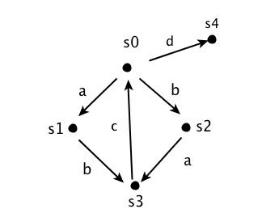
\includegraphics[scale = 0.5]{img/ste.jpg}
    \caption{Esempio di sistema di transizione etichettato}
  \end{figure}
\end{definizione}
La critica di Petri è che in un sistema distribuito non sia individuabile uno
\textbf{stato globale}, che in un sistema distribuito le trasformazioni di stato
siano \textbf{localizzate} e non globali, che non esista un sistema di
riferimento temporale unico (si possono avere più assi temporali in un sistema
distribuito). Quindi la simulazione sequenziale non deterministica (emantica a
``interleaving'') dei sistemi distribuiti è una forzatura e non rappresenta le
reali caratteristiche del comportamento del sistema, ovvero la località, la
distribuzione degli eventi e la relazione di dipendenza causale e non causale
tra gli eventi.
\section{Sistemi Elementari}
Per introdurre i sistemi elementari delle reti di Petri, ovvero una classe molto
semplice e astratta partiamo da un esempio:
\begin{esempio}
  Vediamo l'esempio del \textit{Produttore e del Consumatore}.\\
  Si ha un sistema con una componente Produttore che produce elementi e li
  deposita in un buffer che ha un'unica posizione (quindi o è pieno o è vuoto) e
  con un consumatore che preleva dal buffer un elemento per poi consumarlo ed
  essere pronto a prelevare un altro elemento. Si ha un comportamento
  ciclico. Usiamo quindi le reti di Petri, col modello dei sistemi elementari,
  per rappresentare questo modello. Bisogna quindi individuare le proprietà
  fondamentali locali del sistema.\\
  Partiamo dal produttore, che può avere 2 stati locali:
  \begin{enumerate}
    \item pronto per produrre
    \item pronto per depositare
  \end{enumerate}
  Usiamo i \textbf{cerchi} per rappresentare condizioni locali che sono
  associabili a delle proposizioni della logica che possono essere vere o
  false. Queste preposizioni sono quindi stati locali. Gli eventi locali vengono
  invece rappresentati con un \textbf{rettangolo}. Un evento ha un arco entrante
  da uno stato che rappresenta le \textit{precondizioni} di quell'evento (che
  devono essere vere per permettere l'occorrenza dell'evento). L'occorrenza
  dell'evento rende false le precondizioni e rende vere le
  \textit{postcondizioni} (che sono stati raggiungibili con un arco uscente da
  un evento). Si ha quindi che il produttore può depositare solo se il buffer
  non è pieno, quindi le postcondizioni di un evento devono essere false
  affinché l'evento possa occorrere (oltre alle precondizioni vere).\\
  Passiamo al consumatore che estrae solo se il buffer è pieno ed è pronto a
  prelevare. Si procede poi con la stessa logica del produttore di cambiamento
  tra vero e falso delle varie condizioni locali.\\
  In questo esempio si hanno quindi condizioni che sono preposizioni booleane e
  rappresentano stati locali.
  \begin{figure}[H]
    \centering
    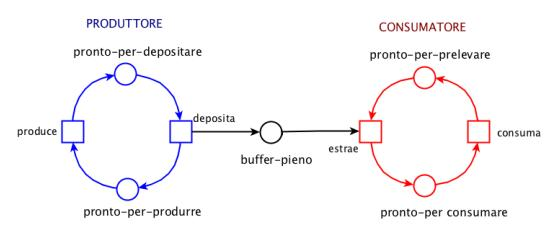
\includegraphics[scale = 0.7]{img/prod.jpg}
    \caption{Produttore e Consumatore}
  \end{figure}
  Lo stato globale del sistema è dato da una
  collezione di stati locali. Per segnare tali condizioni mettiamo un punto
  pieno dentro il cerchio e queste condizioni ``abilitano'' i vari eventi:
  \begin{figure}[h]
    \centering
    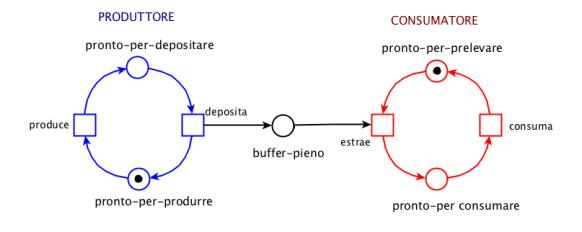
\includegraphics[scale = 0.7]{img/prod1.jpg}
    \caption{Uno stato globale Produttore e Consumatore dove l’evento\textit{
        produce} è l’unico abilitato} 
  \end{figure}
  Si può arrivare ad una \textit{configurazione} dove, per esempio, sia l'evento
  \textit{produce}, del produttore, che l'evento \textit{preleva}, del
  consumatore, sono abilitati. Si ha quindi che i due eventi possono occorrere
  in modo \textbf{concorrente} infatti i due eventi sono \textbf{indipendenti}
  in quanto condizionati da \textbf{precondizioni e postcondizioni completamente
    disgiunte}. Due eventi che occorrono in maniera concorrente lo possono fare in
  qualsiasi ordine, non si ha infatti una sequenza temporale specifica tra i
  due. \\
  In questo sistema quindi siano solo stati locali ed eventi localizzati e non
  stati ed eventi globali. Un evento dipende solo dalle sue precondizioni e
  dalle sue postcondizioni.\\
  \textit{Se rappresentiamo con delle marche le condizioni vere possiamo
    simulare il comportamento del sistema con il \textit{gioco delle marche} che
    mostra come l'evoluzione delle condizioni avviene all'occorrenza degli
    eventi.} \\
  La simula di un tale sistema può comunque avvenire con un sistema di
  transizioni etichettato, ovvero con un automa a stati finiti, che rappresenta
  gli stati globali corrispondenti alle diverse combinazioni di stati locali che
  di volta in volta sono veri. Gli archi vengono etichettati con gli eventi che
  comportano un cambiamento di stato globale:
  \begin{figure}[H]
    \centering
    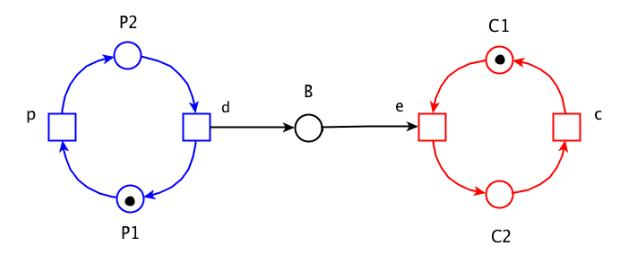
\includegraphics[scale = 0.4]{img/prod3.jpg}
    \caption{Semplificazione della nomenclatura del sistema per praticità}
    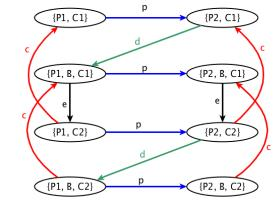
\includegraphics[scale = 0.8]{img/prod2.jpg}
    \caption{Rappresentazione del sistema con un automa a stati finiti che
      rappresenta stati globali}
  \end{figure}
\end{esempio}
Passiamo ora alla formalizzazione di questi aspetti.\\
\begin{definizione}
  Una \textbf{rete elementare} è definita come una tripla:
  \[N=(B,E,F)\]
  dove:
  \begin{itemize}
    \item $B$ è un insieme finito di \textbf{condizioni}, ovvero \textit{stati
      locali}, preposizioni booleane etc$\ldots$. Vengono rappresentate con un
    cerchio 
    \item $E$ è un insieme finito di \textbf{eventi}, ovvero trasformazioni
    locali di stato e \textit{transizioni locali}. Vengono rappresentate con un
    quadrato 
    \item $F$ è una \textbf{relazione di flusso} che connette condizioni ad
    eventi ed eventi a condizioni. Si ha quindi che:
    \[F\subseteq (B\times E)\cup(E\times B)\]
    Le relazioni di flusso sono rappresentate da archi orientati. Inoltre la
    relazione di flusso è tale per cui non esistano \textbf{elementi isolati},
    in quanto non avrebbero senso, in un tale sistema, eventi isolati (che non
    modificherebbero mai una condizione) o condizioni isolate (che non
    verrebbero mai modificate da un evento). Si ha, formalmente, che: 
    \[dom(F)\cup ran(F)=B\cup E\]
    \textbf{chiedere per formula sopra}
  \end{itemize}
  Si ha che:
  \[B\cap E = \emptyset\]
  \[B\cup E \neq \emptyset\]
  Ovvero gli insiemi delle condizioni e degli eventi sono tra loro disgiunti e
  non vuoti.\\
  Sia ora $x$ un elemento qualsiasi della rete, ovvero $x$ può essere o una
  condizione o un evento, formalmente:
  \[x\in B\cup E\]
  si ha che:
  \begin{itemize}
    \item $^\bullet x=\{y\in X:\,(y,x)\in F\}$ rappresenta l'insieme di tutti gli
    elementi $y$ che sono connessi dalla relazione di flusso ad $x$, ovvero si
    ha un arco da $y$ a $x$. Sono quindi i \textbf{pre-elementi} di $x$, ovvero
    le \textit{precondizioni}, se $x$ è un evento, o i \textit{pre-eventi}, se
    $x$ è una condizione
    \item $x^\bullet=\{y\in X:\,(x,y)\in F\}$ rappresenta l'insieme di tutti gli
    elementi $y$ che sono connessi dalla relazione di flusso a partire da $x$,
    ovvero si ha un arco da $x$ a $y$. Sono quindi i \textbf{post-elementi} di
    $x$, ovvero le \textit{postcondizioni}, se $x$ è un evento, o i
    \textit{post-eventi}, se $x$ è una condizione
  \end{itemize}
  Posso estendere questa notazione ad insiemi di elementi. Sia $A$ un insieme
  qualsiasi di elementi, che possono quindi essere sia condizioni che eventi:
  \[A\subseteq B\cup E\]
  Si ha quindi che i pre-elementi dell'insieme $A$ sono rappresentati con:
  \[^\bullet A=\cup_{x\in A} ^\bullet x\]
  ovvero l'unione dei pre-elementi di ogni singolo elemento dell'insieme $A$.\\
  Analogamente si ha che i post-elementi dell'insieme $A$ sono rappresentati
  con: 
  \[A^\bullet=\cup_{x\in A} x^\bullet\]
  ovvero l'unione dei post-elementi di ogni singolo elemento dell'insieme $A$.
  \textit{Nelle reti c'è sempre una relazione di \textbf{dualità} tra due elementi, per
    esempio tra condizioni ed eventi, tra pre-eventi e post-eventi, tra
    pre-condizioni e post-condizioni. Inoltre si ha la caratteristica della
    \textbf{località}, quindi si hanno stati locali e trasformazioni di stato
    locali}
\end{definizione}
La rete $N=(B,E,F)$ descrive la \textit{struttura statica del sistema}, il
comportamento é definito attraverso le nozioni di \textbf{caso (o
  configurazione)} e di \textbf{regola di scatto (o di transizione)}.\\
Una rete può anche essere suddivisa in sotto-reti, seguendo l'esempio sopra si
potrebbe avere una sotto-rete per il produttore, una per il consumatore e anche
una per il buffer.\\
\begin{definizione}
  Un \textbf{caso} (o \textbf{configurazione}) é un insieme di condizioni
  $c\subseteq B$ che rappresentano l’insieme di condizioni vere in una certa
  configurazione del sistema, un insieme di \textbf{stati locali} che
  collettivamente individuano lo \textbf{stato globale} del sistema.\\
  Graficamente le condizioni vere presentano un puntino in mezzo al cerchio
  mentre le condizioni false solo un cerchio vuoto
\end{definizione}
\begin{definizione}
  Sia $N=(B,E,F)$ una rete elementare e sia $c\subseteq B$ una certa
  configurazione (non serve quindi necessariamente conoscere tutto lo stato del
  sistema). La \textbf{regola di scatto} mi permette di stabilire quando
  un evento $e\in E$ è abilitato, ovvero può occorrere, in $c$ sse:
  \[^\bullet e\subseteq c \mbox{ e } e^\bullet \cap c = \emptyset\]
  ovvero sse tutte le precondizioni dell'evento sono vere (e quindi sono
  contenute nella configurazione $c$) e sse tutte le postcondizioni sono false
  (quindi non si hanno intersezioni tra le postcondizioni e la
  configurazione). \\
  L'occorrenza (l'abilitazione) di $e$ in $c$ si denota con la scrittura:
  \[c[e >\]
  Se un evento $e$ è abilitato in $c$, ovvero $c[e >$, si ha che quando $e$
  occorre in $c$ genera un nuovo caso $c'$ e si usa la notazione:
  \[c[e > c'\]
  Si ha quindi che $c'$ è così calcolabile:
  \[c'=(c-^\bullet e)\cup e^\bullet\]
  Ovvero togliendo da $c$ tutte le precondizioni dell'evento $e$ e aggiungendo
  quindi tutte le postcondizioni di $e$
\end{definizione}
Le reti si basano sul \textbf{principio di estensionalità}, ovvero sul fatto che
il cambiamento di stato è locale:
\begin{center}
  \textit{un evento è completamente caratterizzato dai cambiamenti che produce
    negli stati locali, tali cambiamenti sono indipendenti dalla particolare
    configurazione in cui l’evento occorre.}
\end{center}
L'importante è che le precondizioni di un evento siano vere e le postcondizioni
false (siamo comunque interessati solo alla validità delle condizioni che
riguardano l'evento).
\newpage
\begin{esempio}
  Vediamo un esempio esplicativo dove l’evento $e$ è l'unico abilitato, ovvero
  le sue precondizioni sono vere e le sue postcondizioni sono false.\\
  Lo scatto di $e$ rende le precondizioni false e le postcondizioni vere,
  mentre le altre condizioni rimangono inalterate:
  \begin{figure}[H]
    \centering
    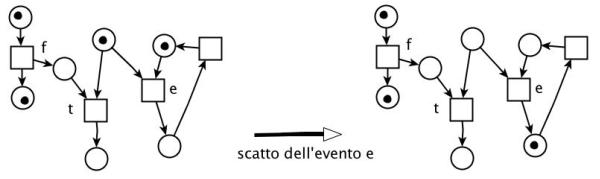
\includegraphics[scale = 0.6]{img/est.jpg}
  \end{figure}
  Si nota quindi che lo scatto dell'evento $e$ riguarda solo le precondizioni e
  le postcondizioni di quel dato evento, come ci ricorda il principio di
  estensionalità 
\end{esempio}
\begin{definizione}
  Sia $N=(B,E,F)$ una rete elementare. Possiamo definire due tipologie di rete:
  \begin{enumerate}
    \item $N$ è definita \textbf{semplice} sse:
    \[\forall x,y \in B\cup E,\,\, (^\bullet x = ^\bullet y)\wedge (x^\bullet =
      y^\bullet)\Rightarrow x = y\]
    Ovvero per ogni coppia di elementi (che siano quindi eventi o condizioni) se
    i loro pre-elementi e i loro post-elementi coincidono allora non ha senso
    distinguere $x$ e $y$.
    \begin{figure}[H]
      \centering
      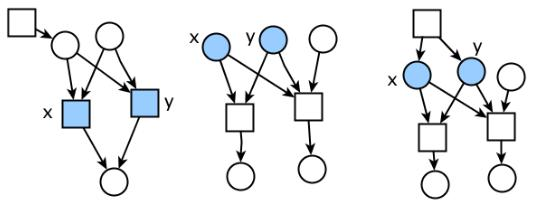
\includegraphics[scale = 0.5]{img/sem.jpg}
      \caption{Esempi di reti \textbf{non} semplici}
    \end{figure}
    \newpage
    \item $N$ è definita \textbf{pura} sse:
    \[\forall e \in E:\,\,^\bullet e \cap e^\bullet = \emptyset\]
    Ovvero se per ogni evento non esiste una precondizione che sia anche
    postcondizioni. Si ha quindi un \textbf{cappio} (detto anche \textbf{side
      condition}) tra un evento e una condizione. Avere questa situazione
    comporta che l'evento non può scattare in quanto la condizione che per lui è
    sia una precondizione che una postcondizioni non può essere
    contemporaneamente vera e falsa, l'evento non potrà mai scattare e quindi
    non potrà mai essere osservato. Non avrebbe quindi senso modellarlo
    \begin{figure}[H]
      \centering
      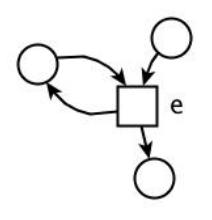
\includegraphics[scale = 0.5]{img/pura.jpg}
      \caption{Esempio di rete \textbf{non} pura}
    \end{figure}
  \end{enumerate}
\end{definizione}
\begin{definizione}
  Data una rete elementare $N=(B,E,F)$ e sia $U \subseteq E$ un sottoinsieme di
  eventi e siano $c,c_1,c_2\in B$ tre configurazioni. Si ha che:
  \begin{itemize}
    \item $U$ è un \textbf{insieme di eventi indipendenti} sse:
    \[\forall e_1,e_2\in U:\,\,e_1\neq e_2\Rightarrow (^\bullet e_1\cup
      e_1^\bullet)\cap  (^\bullet e_2\cup e_2^\bullet) = \emptyset\]
    ovvero per ogni coppia distinta di eventi nell'insieme $U$ si ha che le
    precondizioni e le postcondizioni dei due eventi sono completamente
    disgiunte.
    \item $U$ è un \textbf{passo abilitato}, ovvero un insieme di \textit{eventi
      concorrenti} in una certa configurazione $c$, che si indica con:
    \[c[U>\]
    sse:
    \[U \mbox{ è un insieme di eventi indipendenti } \wedge\,\, \forall e\in
      U:\,\, c[e>\]
    $U$ quindi deve essere un insieme di eventi indipendenti e ogni evento in
    $U$ è abilitato in $c$, quindi le sue precondizioni sono vere e le sue
    postcondizioni sono false. Si ha quindi che $U$ è un insieme di eventi
    abitati in maniera concorrente in $c$
    \item $U$ è un \textbf{passo} dalla configurazione $c_1$ alla configurazione
    $c_2$, che si indica con:
    \[c_1[U > c_2\]
    sse:
    \[(c_1[U) \wedge \Big(c_2=(c_1-^\bullet U)\cup U^\bullet\Big)\]
    ovvero sse $U$ è un passo abilitato in $c_1$ e lo scatto degli eventi in $U$
    porta alla configurazione $c_2$ che si ottiene togliendo da $c_1$ l'insieme
    delle precondizioni degli eventi in $U$ e aggiungendo quindi l'insieme delle
    postcondizioni degli eventi in $U$
  \end{itemize}
\end{definizione}
\begin{esempio}
  Riprendiamo l'esempio del produttore e del consumatore.\\
  Sia dato il sistema $\Sigma$ che modella produttore e consumatore
  \begin{figure}[H]
    \centering
    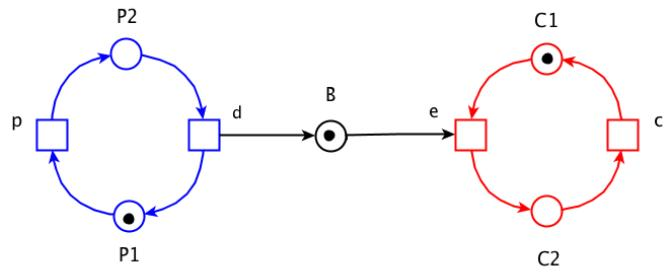
\includegraphics[scale = 0.6]{img/prod5.jpg}
  \end{figure}
  Si hanno:
  \begin{itemize}
    \item $\{p,e\},\{p,c\},\{d,c\}$ esempi di insiemi di eventi indipendenti
    \item $\{p,e\}$ che è un passo abilitato in $\{P_1,B,C_1\}$
    \item $\{P_1,B,C_1\}[\{p,w\}>\{P_2,C_2\}$ ovvero lo scatto del passo
    $\{p,e\}$ ci porta in $\{P_2,C_2\}$
  \end{itemize}
\end{esempio}
Diamo ora una definizione formale di \textbf{sistema elementare}.
\begin{definizione}
  Un \textbf{sistema elementare} $\Sigma=(B,E,F;c_{in})$ è definito come una
  rete $N=(B,E,F)$ e a cui è associato un caso iniziale, una configurazione
  iniziale, ovvero un sottoinsieme di condizioni che rappresentano lo stato
  iniziale da cui inizia la computazione e l'evoluzione del sistema. Formalmente
  il caso iniziale si indica con $C_{in}\in B$ 
\end{definizione}
\begin{definizione}
  Dato un sistema elementare $\Sigma=(B,E,F;c_{in})$ si indica con $C_\Sigma$
  l'insieme dei \textbf{casi raggiungibili} da tale sistema a partire dal caso
  iniziale $c_{in}$.\\
  Formalmente l'insieme dei casi raggiungibili è il di piccolo sottoinsieme
  dell'insieme delle parti di $B$, ovvero $2^B$, tale che:
  \begin{itemize}
    \item $c_{in}\in C_\Sigma$, ovvero sicuramente il caso iniziale appartiene
    all'insieme dei casi raggiungibili
    \item se $c\in C_\Sigma,\,U\subseteq E$ e $c'\subseteq B$ sono tali che
    $c[U>c'$ allora $c'\in C_\Sigma$, ovvero se ho un generico caso $c$ che
    appartiene ai casi raggiungibili, se ho un insieme di eventi $U$ tale che
    questo insieme di eventi (che abbiamo visto essere indipendenti, per la
    definizione di passo abilitato) è abilitato
    in $c$ in un unico passo e la sua occorrenza mi porta in $c'$, allora anche
    $c'$ appartiene a $C_\Sigma$. 
  \end{itemize}
  Questa è una definizione data per \textbf{induzione strutturale}, nel primo
  punto si ha la base, nel secondo l'ipotesi e la conseguenza
\end{definizione}
\begin{definizione}
  Dato un sistema elementare $\Sigma=(B,E,F;c_{in})$ si indica con $U_\Sigma$
  l'\textbf{insieme dei passi} di $\Sigma$, ovvero di tutti i possibili insiemi
  di eventi indipendenti che possono occorrere in qualche caso. Formalmente:
  \[U_\Sigma =\{U\subseteq E\,|\,\exists\, c,c'\in C_\Sigma :\, c[U>c'\}\]
  Ovvero l'insieme dei sottoinsiemi di eventi tali per cui esistano due casi
  raggiungibili in $C_\Sigma$ e $U$ è abilitato in $c$ e il suo scatto mi porta
  in $c'$.
\end{definizione}
Definiamo ora il comportamento dei sistemi elementari.
\begin{definizione}
  Sia $\Sigma=(B,E,F;c_{in})$ un sistema elementare e siano $c_i\in C_\Sigma$ ed
  $e_i\in E$.\\
  Definiamo;
  \begin{itemize}
    \item un \textbf{comportamento sequenziale} come una sequenza di eventi che
    possono occorrere dal caso iniziale. Facendo scattare in maniera sequenziale
    gli eventi uno alla volta in $c_n$:
    \[c_{in} [e_1 > c_1 [e_2 > \ldots[e_n > c_n\]
    Scrittura che può essere alleggerita in:
    \[c_{in} [e_1 e_2 \ldots e_n > c_n\]
    Possiamo dire di avere a che fare con una \textbf{simulazione sequenziale
      non deterministica, detta anche \textit{semantica a interleaving}},
    infatti ho più eventi abilitati da prendere uno alla volta
    \item un \textbf{comportamento non sequenziale}, in quanto possiamo anche
    considerare insiemi di eventi, ovvero passi. Considero quindi sequenze di
    passi, avendo a che fare con la \textbf{step semantics}. Non ho quindi una
    simulazione sequenziale non deterministica in quanto dal caso iniziale
    faccio scattare un insieme di eventi, in maniera concorrente (e quindi senza
    ordine specificato), per poi far scattare un altro insieme di eventi fino ad
    arrivare a $c_n$: 
    \[c_{in} [U_1 > c_1 [U_2 > \ldots [U_n > c_n\]
    Scrittura che può essere alleggerita in:
    \[c_{in} [U_1 U_2 \ldots U_n > c_n\]
    Gli insiemi $U_i$ non sono insiemi massimali abilitati ma sottoinsiemi
    indipendenti e abilitati in $c_{in}$.\\
    Posso avere anche un altro tipo di \textbf{comportamento non sequenziale},
    definito da Petri stesso, in una \textbf{semantica ad ordini parziali} in
    cui si definiscono processi non sequenziali. Il comportamento di tale
    sistema viene registrato in una rete di Petri
  \end{itemize}
  In ogni caso si considerano sia sequenze finite che infinite (con cicli) di
  eventi o passi. 
\end{definizione}
\newpage
\begin{esempio}
  Dato il sistema elementare $\Sigma$:
  \begin{figure}[H]
    \centering
    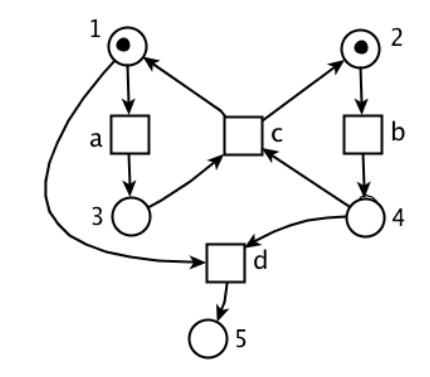
\includegraphics[scale = 0.4]{img/seq.jpg}
  \end{figure}
  si ha, per esempio, la seguente sequenza di occorrenza di eventi:
  \[\{1, 2\}[a > \{3, 2\}[b > \{3, 4\}[c > \{1, 2\}[b > \{1, 4\}[d > \{5\}\]
  arrivati in ``5'' abbiamo un caso finale, ovvero una situazione di
  \textbf{deadlock}, in quanto il sistema non può evolvere ulteriormente.\\
  Vediamo anche la seguente possibile sequenza di passi. In ``1'' e ``2'' sia
  ``a'' che ``b'' sono indipendenti e sono entrambi abilitati (scattano in
  maniera concorrente in un unico passo$\ldots$ ovviamente posso avere passi con lo
  scatto di un solo evento):
  \[\{1, 2\}[\{a, b\} > \{3, 4\}[\{c\} > \{1, 2\}[\{b\} > \{1, 4\}\]
  Come ricordato posso finire in una sequenza infinita.
\end{esempio}
Vediamo ora come modellare e registrare il comportamento del sistema. Un modo è
usando il \textbf{grafo dei casi raggiungibili}.
\begin{definizione}
  Il \textbf{grafo dei casi raggiungibili} di un sistema elementare
  $\Sigma=(B,E,F;c_{in})$ è il sistema di transizioni etichettato:
  \[CG_\Sigma=(C_\Sigma, U_\Sigma, A, c_{in})\]
  dove:
  \begin{itemize}
    \item $C_\Sigma$ è l'insieme dei nodi del grafo, ovvero gli stati globali
    sono i casi raggiungibili dal sistema $\Sigma$    
    \item $U_\Sigma$, è l'alfabeto, ovvero i passi del sistema rappresentano
    l'alfabeto 
    \item $A$ è l'insieme di archi etichettati, formalmente definito come:
    \[A=\{(c,U',c')|\,c,c'\in C_\Sigma, U\in U_\Sigma, c[U>c']\}\]
    ovvero sono archi che connettono uno caso $c$ con un caso $c'$ e sono
    etichettati con un passo $U$ sse $U$ è abilitato in $c$ e porta in
    $c'$. Ovviamente $c$ e $c'$ sono devono essere raggiungibili e $U$ deve
    appartenere all'insieme dei passi di $\Sigma$
  \end{itemize} 
\end{definizione}
\begin{figure}[H]
  \centering
  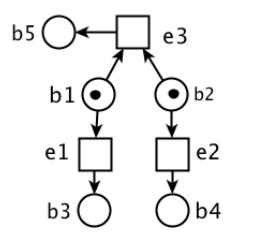
\includegraphics[scale = 0.5]{img/seq1.jpg}
  \caption{il sistema $\Sigma$}
  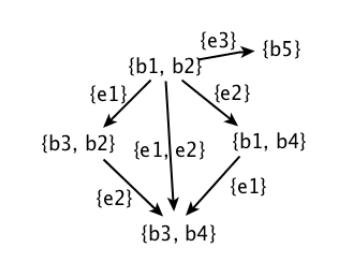
\includegraphics[scale = 0.5]{img/seq2.jpg}
  \caption{Grafo dei casi del sistema $\Sigma$}
\end{figure}
\newpage
\subsection{Diamond Property}
Dato un sistema elementare $\Sigma = (B,E,F;c_{in})$ e il suo grafo dei casi
$CG_\Sigma=(C_\Sigma, U_\Sigma, A, c_{in})$ si ha 
che il grafo soddisfa una particolare proprietà, detta \textbf{diamond
  property}, tipica solo dei sistemi elementari.
\begin{definizione}
  La \textbf{diamond property} stabilisce una proprietà della struttura del
  grafo della rete elementare, ovvero, dati $U_1,U_2\in U_\Sigma$ tali che:
  \begin{itemize}
    \item $U_1\cap U_2=\emptyset$
    \item $U_1\neq\emptyset$
    \item $U_2\neq\emptyset$
  \end{itemize}
  e dati $c_i\in C_\Sigma$ allora vale, per esempio:
  \begin{figure}[H]
    \centering
    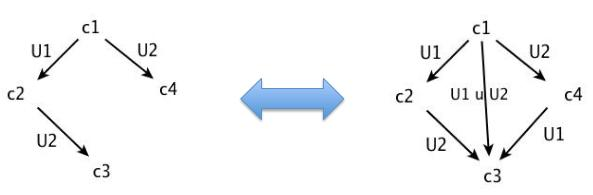
\includegraphics[scale = 0.6]{img/diam.jpg}
  \end{figure}
  ovvero se posso rilevare come sottografo una struttura come quella a sinistra
  nell'immagine allora sicuramente tale sottografo contiene anche l'arco gli
  archi per ottenere l'immagine di destra. Il discorso vale anche all'opposto.
\end{definizione}
Si possono fare delle prove:
\begin{enumerate}
  \item \textbf{prima prova:}\\
  Dimostriamo che possiamo passare all'immagine di destra da quella di sinistra
  aggiungendo i due archi mancanti.\\
  Per semplicità diciamo che $U_i$ è un singolo evento $e_i$, con $i=1,2$. Siano
  inoltre $c_1,c_2\in C_\Sigma$, ovvero sono casi raggiungibili, ed $e_1,e_2\in
  E$ tali che $c_1 [e_1 > c_2 [e_2 > \mbox{ e } c_1 [e_2 >$, i due eventi quindi
  sono abilitati in sequenza e da $c_1$ è anche abilitato $c_2$ . Si vuole
  dimostrare che: 
  \[(^\bullet e_1\cup e_1^\bullet)\cap(^\bullet e_2\cup e_2^\bullet)=\emptyset\]
  ovvero che i due eventi sono indipendenti, che sono entrambi abilitati e che
  sono eseguibili in qualsiasi ordine.
  \newpage
  Da $c_1 [e_1 > \mbox{ e }c_1 [e_2 >$ segue che:
  \begin{itemize}
    \item $^\bullet e_1\cap e_2^\bullet=\emptyset$
    \item $^\bullet e_2\cap e_1^\bullet=\emptyset$
  \end{itemize}
  infatti se $e_1$ e $e_2$ sono entrambi abilitati in $c_1$, le loro
  pre-condizioni sono vere e le post-condizioni false, e quindi non è possibile
  che una condizione sia contemporaneamente precondizione di $e_1$ (vera) e
  anche postcondizione di $e_2$ (falsa), e viceversa. Quindi le precondizioni
  di un evento sono disgiunte dalle postcondizioni dell'altro.\\
  Inoltre dal fatto che ho $c_1 [e_1 > c_2 [e_2$, ovvero che da $c_1$ è
  abilitato $e_1$ e che dopo lo scatto di $e_1$ è ancora abilitato $e_2$
  possiamo dire che:
  \begin{itemize}
    \item $e_1^\bullet\cap e_2^\bullet=\emptyset$
    \item $^\bullet e_1\cap\, ^\bullet e_2=\emptyset$
  \end{itemize}
  in $c_2$, infatti, le pre-condizioni di $e_1$ sono false mentre le
  precondizioni di $e_2$ sono vere e quindi $e_1$ e $e_2$ non possono avere
  precondizioni in comune; inoltre sempre in $c_2$ le postcondizioni di $e_1$
  sono vere, mentre quelle di $e_2$ sono false, e quindi $e_1$ e $e_2$ non
  possono avere post-condizioni in comune. Quindi le precondizioni dei due
  eventi sono disgiunte, come del resto anche le postcondizioni, in quanto i due
  eventi sono sequenziali.\\
  Si è quindi dimostrato che i due eventi hanno precondizioni e postcondizioni
  completamente disgiunte e quindi la tesi è verificata
  \item \textbf{seconda prova:}\\
  Analizzando la situazione:
  \begin{figure}[H]
    \centering
    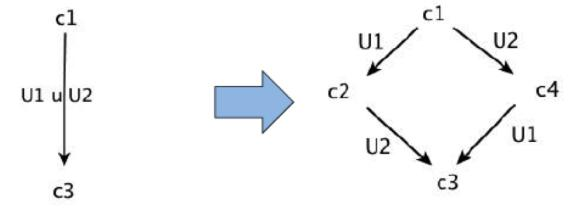
\includegraphics[scale = 0.45]{img/diam2.jpg}
  \end{figure}
  \newpage
  Si supponga che $U_1\cup U_2\in U_\Sigma$ e che si abbiano:
  \begin{itemize}
    \item $U_1\cap U_2=\emptyset$, ovvero sono disgiunti
    \item $U_1\neq\emptyset$
    \item $U_2\neq\emptyset$
  \end{itemize}
  allora se $c_1[(U_1\cup U_2)>c_3$, quindi è abilitato il passo $U_1\cup U_2$
  in $c_1$, sicuramente si ha che sono abilitati anche i singoli passi:
  \begin{itemize}
    \item $c_1[U_1>$
    \item $c_1[U_2>$
  \end{itemize}
  resta da dimostrare che dopo lo scatto di $U_1$ è ancora abilitato $U_2$ in
  $c_2$. Ma se $U_1\cup U_2$ è un passo abilitato significa che posso eseguirli
  in qualsiasi ordine, quindi anche prima $U_1$ e poi $U_2$, e questo comporta
  sicuramente che $U_2$ è abilitato e che porta a $c_3$. Analogamente invertendo
  $U_1$ e $U_2$, formalmente: 
  \begin{itemize}
    \item $c_1[U_1>c_2[U_2>c_3$
    \item $c_1[U_2>c_4[U_1>c_3$
  \end{itemize}
  Si dimostra così che l'immagine di sinistra comporta quella di destra.
\end{enumerate}
Grazie alla diamond property possiamo non considerare il grafo dei casi
raggiungibili ma solo il \textbf{grafo dei casi sequenziale}:
\begin{definizione}
  Un \textbf{grafo dei casi sequenziale} del sistema elementare
  $\Sigma=(B,E,F;c_{in})$ è una quadrupla:
  \[SCG_\Sigma=(C_\Sigma,E,A,c_{in})\]
  dove le etichette sono i singoli eventi (mentre il resto rimane definito come
  nel grafo dei casi raggiungibili). Formalmente si ha quindi che:
  \[A=\{(c,e,c')|\,c,c'\in C_\Sigma,\,e\in E:\, c[e>c'\}\]
  \begin{figure}[H]
    \centering
    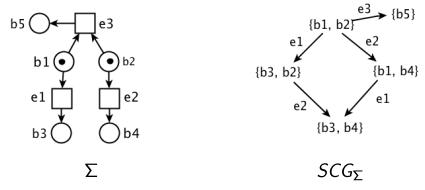
\includegraphics[scale = 0.5]{img/seq3.jpg}
    \caption{Esempio di grafo dei casi sequenziale}
  \end{figure}
  Si registra quindi l'occorrenza di un evento alla volta. Il grafo dei casi
  sequenziale è quindi il sistema di transizione con gli archi etichettati dai
  singoli eventi.
  \begin{figure}[H]
    \centering
    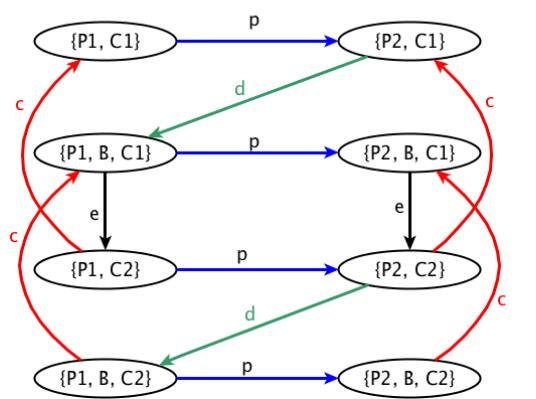
\includegraphics[scale = 0.4]{img/seqq.jpg}
    \caption{Esempio di grafo dei casi sequenziale dell'esempio c0on produttore
      e consumatore}
  \end{figure}
\end{definizione}
Riprendendo l'immagine precedente si ha che per la diamond property possono
aggiungere l'arco ``centrale'' che trasformerebbe nuovamente il grafo dei casi
sequenziale in quello dei casi raggiungibili quindi:
\textit{per la diamond property, nei sistemi elementari il grafo dei casi e il
  grafo dei casi sequenziale sono \textbf{sintatticamente equivalenti}, ovvero
  possono essere ricavati a vicenda.\\
  Questo implica il fatto che due sistemi elementari hanno grafi dei casi
  \textbf{isomorfi} sse hanno grafi dei casi sequenziali isomorfi.}
\subsection{Isomorfismo tra Sistemi di Transizione Etichettati}
Si ricorda che:
\begin{center}
  \textit{Si parla di isomorfismo quando due strutture complesse si possono
    applicare l'una sull'altra, cioè far corrispondere l'una all'altra, in modo
    tale che per ogni parte di una delle strutture ci sia una parte
    corrispondente nell'altra struttura; in questo contesto diciamo che due
    parti sono corrispondenti se hanno un ruolo simile nelle rispettive
    strutture.}
\end{center}
Diamo ora una definizione formale di isomorfismo tra sistemi di transizione
etichettati, che possono quindi essere grafi dei casi o grafi dei casi
sequenziali.
\begin{definizione}
  Siano dati due sistemi di transizione etichettati:\\
  $A_1 = (S_1,E_1,T_1,s_{01})$ e $A_2 = (S_2 , E_2 , T_2 , s_{02})$.\\
  e siano date due \textbf{mappe biunivoche}:
  \begin{enumerate}
    \item $\alpha:S_1\to S_2$, ovvero che passa dagli stati del primo sistema a
    quelli del secondo
    \item $\beta:E_1\to E_2$, ovvero che passa dagli eventi del primo sistema a
    quelli del secondo
  \end{enumerate}
  allora:
  \[\langle \alpha,\beta\rangle:A_1= (S_1 , E_1 , T_1 ,s_{01})\to A_2 = (S_2 ,
    E_2 , T_2 , s_{02})\]
  è un \textbf{isomorfismo} sse:
  \begin{itemize}
    \item $\alpha(s_{01})=s_{02}$, ovvero l'immagine dello stato iniziale del
    primo sistema coincide con lo stato iniziale del secondo
    \item $\forall s,s'\in S_1,\forall e\in E_1:\,(s,e,s')\in T_1
    \Leftrightarrow (\alpha(s),\beta(e),\alpha(s'))\in T_2$ ovvero per ogni
    coppia di stati del primo sistema, tra cui esiste un arco etichettato $e$,
    vale che esiste un arco, etichettato con l'immagine di $e$, nel secondo
    sistema che va dall'immagine del primo stato considerato del primo sistema
    all'immagine del secondo stato considerato del secondo sistema, e viceversa
  \end{itemize}
\end{definizione}
\begin{definizione}
  Si definiscono due \textbf{sistemi equivalenti} sse hanno grafi dei casi
  sequenziali, e quindi di conseguenza anche grafi dei casi, \emph{isomorfi}.\\
  Due sistemi equivalenti accettano ed eseguono le stesse sequenze di eventi
\end{definizione}
\subsection{Il Problema della Sintesi}
Si presenta ora un problema tipico dell'informatica, il \textbf{problema della
  sintesi}, ovvero dato un comportamento, o meglio una sua specifica, decidere
se esiste un'implementazione di tale specifica, ovvero un modello, che abbia
esattamente quel comportamento.\\
In questo caso dato un sistema di transizioni etichettato $A=(S,E,T,s_0)$, con:
\begin{itemize}
  \item $S$ insieme degli stati
  \item $E$ insieme delle etichette, ovvero degli eventi
  \item $T$ insieme delle transizioni
  \item $s_0$ stato iniziale
\end{itemize}
ci si propone di stabilire se esiste un sistema elementare
$\Sigma=(B,E,F;c_{in})$, tale che l'insieme degli eventi del sistema esattamente
l'insieme delle etichette di $A$ e tale che il suo grafo dei casi $SCG_\Sigma$
sia isomorfo ad $A$. Ci si propone anche di costruirlo.\\
Il problema è stato risolto mediante la cosiddetta \textbf{teoria delle regioni}
(che però non verrà trattato nel corso). Si può però dire che $A$ dovrà
soddisfare la diamond property, in quanto altrimenti non sarebbe un sistema di
transizioni che potrebbe corrispondere al comportamento di un sistema
elementare.
\subsection{Contatti}
\begin{definizione}
  Sia $\Sigma = (B,E,F;c_{in})$ un sistema elementare e siano $e\in E$ un evento
  e $c\in C_\Sigma$ un caso raggiungibile dal caso iniziale. Allora si ha che
  $(e,c)$ è un \textbf{contatto} sse:
  \[^\bullet e\subseteq c \wedge e^\bullet \cap c \neq\emptyset\]
  Ovvero, in termini pratici, siamo nel caso in cui un evento $e$ ha le
  precondizioni vere, si ha quindi che $^\bullet e\subseteq c$, e l'evento non
  ha tutte le postcondizioni false, quindi $e^\bullet \cap c \neq\emptyset$,
  allora si dice che l'evento $e$ è in una situazione di contatto e quindi non
  può scattare
  \begin{figure}[H]
    \centering
    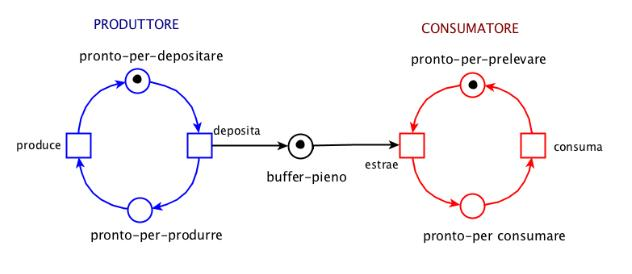
\includegraphics[scale = 0.6]{img/con.jpg}
    \caption{Esempio dove l'evento \emph{deposita} è in una situazione di
      contatto}
  \end{figure}
\end{definizione}
\begin{definizione}
  Sia $\Sigma = (B,E,F;c_{in})$ un sistema elementare. Si dice che il sistema è
  \textbf{senza contatti} sse:
  \[\forall e\in E,\,\forall c\in C_\Sigma\mbox{ si ha che } ^\bullet
    e\subseteq c\Rightarrow e^\bullet\cap c=\emptyset\]
  ovvero per ogni evento e per ogni caso raggiungibile dal caso iniziale succede
  sempre che se le precondizioni sono vere, ovvero $^\bullet e\subseteq c$,
  allora le postcondizioni sono false, ovvero disgiunte dal caso considerato
  ($e^\bullet\cap c=\emptyset$)
\end{definizione}
Ci si chiede se sia possibile trasformare un sistema elementare $\Sigma$, con
contatti, in uno $\Sigma'$, senza contatti, senza però modificarne il
comportamento.\\
La risposta a questo quesito è affermativa e la procedura consiste
nell'aggiungere a $\Sigma$ il complemento di ogni condizione che crea situazione
di contatto, ottenendo così un sistema $\Sigma'$ con grafo dei casi isomorfo a
quello di $\Sigma$.\\ 
Per aggiungere il complemento, data la condizione $x$, si aggiunge la condizione
$not\,\, x$ che sarà vera tutte le volte che $x$ è falsa e viceversa. Per
ottenere questo risultato la nuova condizione avrà come pre-eventi i
post-eventi di $x$ e come post-eventi i pre-eventi di $x$. Ovvero
connetto la nuova condizione agli stessi eventi di quella vecchia ma con archi
orientati in senso opposto. Ovviamente le inizializzazioni delle due condizioni
dovranno essere opposte (una vera e l'altra falsa).
\begin{figure}[H]
  \centering
  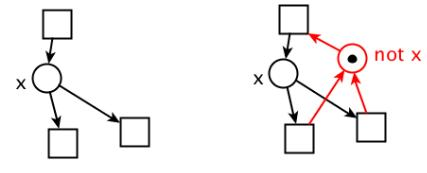
\includegraphics[scale = 0.6]{img/con2.jpg}
  \caption{Esempio con l'ottenimento del complemento di un sistema}
\end{figure}
Se un sistema è senza contatti si ha una regola di contatto semplificata:
\begin{definizione}
  Sia $\Sigma = (B,E,F;c_{in})$ un sistema elementare \textbf{senza
    contatti}. Sapendo che se le precondizioni di un evento sono vere allora
  sicuramente le postcondizioni di quell'evento sono false in quel caso. Dato
  che questo avviene per ogni evento e per ogni caso raggiungibile dal caso
  iniziale per verificare che un evento $e$ sia abilitato in un caso
  raggiungibile $c$ è sufficiente verificare che le precondizioni di $e$ siano
  vere (in quanto automaticamente le postcondizioni saranno false). In
  maniera formale quindi si ha che: 
  \[c[e\mbox{ sse } ^\bullet e\subseteq c,\,\,\mbox{ con } e\in E,c\in
    C_\Sigma\]
  semplificando di molto la \textbf{regola di scatto}
\end{definizione}
\begin{figure}[H]
  \centering
  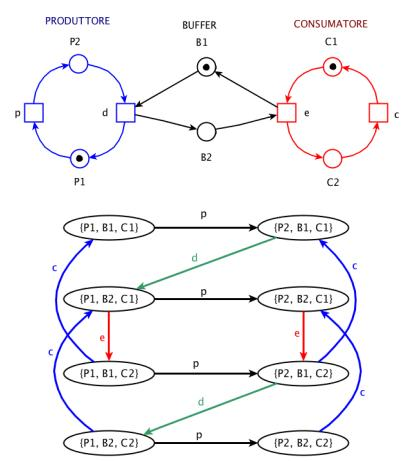
\includegraphics[scale = 0.6]{img/con3.jpg}
  \caption{Esempio con il complemento del sistema produttore-consumatore (dove è
    stato aggiunto solo il complemento di ``buffer-pieno'', ottenendo così sia
    $B1$ che $B2$, in quanto le altre condizioni avevano già il loro
    complemento). In aggiunta si ha anche il grafo dei casi sequenziale
    corrispondente al nuovo sistema senza contatti (grafo che è isomorfo a
    quello ottenibile al sistema con contatti)} 
\end{figure}
\subsection{Situazioni Fondamentali}
\subsubsection{Sequenza}
\begin{definizione}
  Sia $\Sigma = (B,E,F;c_{in})$ un sistema elementare, con contatti o meno
  e siano $c\in C_\Sigma$ un caso raggiungibile dal caso iniziale e $e_1,e_2\in
  E$ due eventi.\\
  Si ha che $e_1$ ed $e_2$ sono \textbf{in sequenza} nel caso
  raggiungibile $c$ sse:
  \[c[e_1>\wedge\, \neg c[e_2\wedge c[e_1e_2>\]
  ovvero in $c$ è abilitato $e_1$ ma non $e_2$ ma, dopo lo scatto di $e_1$,
  $e_2$ diventa abilitato. Quindi in $c$ è possibile attivare prima $e_1$ e poi
  $e_2$ in sequenza.\\
  Si ha quindi una relazione di \textbf{dipendenza causale tra $e_1$ ed $e_2$},
  ovvero qualche postcondizione di $e_1$ è precondizione di $e_2$ (che quindi
  può occorrere solo se precedentemente è occorso $e_1$).
  \begin{figure}[H]
    \centering
    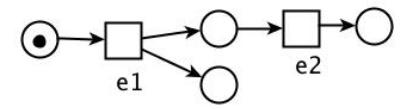
\includegraphics[scale = 0.6]{img/se.jpg}
    \caption{Esempio di sequenza tra $e_1$ ed $e_2$}
  \end{figure}
\end{definizione}
\subsubsection{Concorrenza}
\begin{definizione}
  Sia $\Sigma = (B,E,F;c_{in})$ un sistema elementare, con contatti o meno
  e siano $c\in C_\Sigma$ un caso raggiungibile dal caso iniziale e $e_1,e_2\in
  E$ due eventi. \\
  Si ha che i due eventi sono \textbf{concorrenti} nel caso
  raggiungibile $c$ sse:
  \[c[\{e_1,e_2\}>\]
  ovvero se possono essere abilitati in unico passo o, detto in maniera
  diversa, se sono indipendenti ed entrambi abilitati in $c$
  \begin{figure}[H]
    \centering
    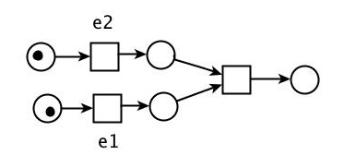
\includegraphics[scale = 0.7]{img/conc.jpg}
    \caption{Esempio di concorrenza tra $e_1$ ed $e_2$}
  \end{figure}
\end{definizione}
\subsubsection{Conflitto}
\begin{definizione}
  Sia $\Sigma = (B,E,F;c_{in})$ un sistema elementare, con contatti o meno
  e siano $c\in C_\Sigma$ un caso raggiungibile dal caso iniziale e $e_1,e_2\in
  E$ due eventi.\\
  Si ha che $e_1$ ed $e_2$ sono in conflitto sse:
  \[c[e_1>\wedge c[e_2 \wedge\,\neg c[\{e_1,e_2\}>\]
  ovvero i due eventi sono entrambi abilitati (quindi le precondizioni sono vere
  mentre le postcondizioni son false) ma l'occorrenza di uno disabilità
  l'altro, quindi non possono essere abilitati in un unico passo, in quanto non
  sono indipendenti. Ci sono due casi:
  \begin{enumerate}
    \item i due eventi hanno una precondizione in comune, e in tal caso si parla
    di \textbf{conflitto forward} (ovvero \textit{in avanti})
    \begin{figure}[H]
      \centering
      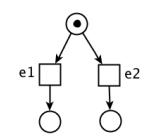
\includegraphics[scale = 0.7]{img/conf1.jpg}
      \caption{Esempio di conflitto forward tra $e_1$ ed $e_2$}
    \end{figure}
    \item i due eventi hanno una postcondizione in comune, e in tal caso si parla
    di \textbf{conflitto backward} (ovvero \textit{all'indietro})
    \begin{figure}[H]
      \centering
      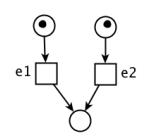
\includegraphics[scale = 0.7]{img/conf2.jpg}
      \caption{Esempio di conflitto backward tra $e_1$ ed $e_2$}
    \end{figure}
  \end{enumerate}
  Si ha quindi una situazione di \textbf{non determinismo}, non essendo
  specificato quale dei due eventi scatterà prima (e lo scatto di uno impedisce
  lo scatto dell'altro).
  \newpage
  Posso ritrovarmi nel caso in cui effettivamente un evento scatta, cambiando lo
  stato del sistema. In tal caso, in un'ottica completamente deterministica, si
  deve assumere che \textbf{l'ambiente} abbia fornito un'informazione
  riguardo il conflitto, ovvero c'è stato qualcosa di esterno che ha permesso ad
  uno dei due eventi di scattare ugualmente. Ho quindi guadagnato
  dell'informazione. 
  \begin{figure}[H]
    \centering
    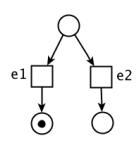
\includegraphics[scale = 0.7]{img/conf3.jpg}
    \caption{Esempio di conflitto con l'intervento dell'ambiente tra $e_1$ ed
      $e_2$ (con conseguente guadagno di informazione)} 
  \end{figure}
  Ci sono però casi in cui in ogni caso non si può avere informazione su quale
  esempio sia scattato. Si può ipotizzare che tale informazione fosse presente
  nello stato precedente del sistema (una sola condizione attiva, per
  esempio). Quindi l'informazione, finita nell'ambiente (ricevuta
  dall'ambiente), si è persa.
  \begin{figure}[H]
    \centering
    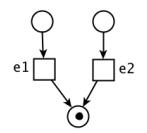
\includegraphics[scale = 0.7]{img/conf4.jpg}
    \caption{Esempio di conflitto tra $e_1$ ed
      $e_2$ con conseguente perdita di informazione (si può ipotizzare, per
      esempio, che nello stato precedente la precondizione di $e_1$ fosse attiva
      mentre quella dio $e_2$ fosse inattiva)} 
  \end{figure}
  Il modello, nell'ottica di Petri, non è quindi un \textbf{modello chiuso} ma è
  in grado di comunicare con l'ambiente (in sintonia con le teorie della
  fisica). 
\end{definizione}
\newpage
\subsubsection{Confusione}
\begin{definizione}
  La situazione di \textbf{confusione} è una \textit{mistura} di situazioni di
  concorrenza e di conflitto. Si hanno 2 tipi di confusione, entrambe
  ammissibili: 
  \begin{enumerate}
    \item detta \textbf{confusione asimmetrica} considera il fatto di avere un
    caso raggiungibile e due eventi abilitati, nella figura $e_1$ ed $e_2$, in
    maniera concorrente in $c$, che nella figura consiste nel caso
    $\{b_1,b_2,b_3\}$. I due eventi sono quindi indipendenti. Nella figura lo
    scatto dei due eventi porterebbe allo stato $c'=\{b_4,b_5\}$. Bisogna
    analizzare però nel dettaglio il sistema. Se prima occorre $e_1$ non si ha
    alcun conflitto mentre se occorre prima $e_2$ (che porterebbe in
    $\{b_1,b_3,b_4\}$) si crea un conflitto tra $e_1$ ed $e_3$, che viene
    risolto a favore di $e_1$ e a sfavore di $e_3$. \textbf{Non è possibile
      stabilire oggettivamente se è stato sciolto un conflitto}. Sono quindi in
    una situazione di confusione in quanto non so se è stata effettuata o meno
    una scelta.
    \begin{figure}[H]
      \centering
      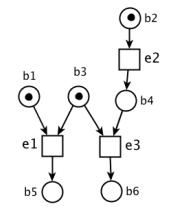
\includegraphics[scale = 0.7]{img/confu.jpg}
      \caption{Esempio di confusione asimmetrica tra $e_1$ ed $e_2$} 
    \end{figure}
    Una soluzione che vedremo sarà la scomposizione in più componenti del
    sistema 
    \item detta \textbf{confusione simmetrica}, nome dovuto al fatto che la rete
    risulta disegnata in modo simmetrico, comportando delle
    problematiche. Prendiamo nell'immagine il caso raggiungibile $c=\{b_1,b_2\}$
    e i due eventi $e_1$ ed $e_3$, abilitati in maniera concorrente. Si ha che
    $c[\{e_1,e_3\}>c'$, con $c'=\{b_3,b_5\}$. Anche in questo caso si hanno dei
    conflitti, infatti sia $e_1$ che $e_3$ sono in conflitto con $e_2$ (in
    quanto se uno dei due viene eseguito $e_2$ non può più occorrere). Anche in
    questo caso non posso stabilire se il conflitto è stato risolto nel momento
    in cui arrivo in $c'$ (ovvero se si è deciso di fare $e_1$ piuttosto che
    $e_2$ o $e_3$ piuttosto che $e_2$).\\
    Anche in questo caso potremo dividere in componenti (una che esegue $e_1$ ed
    $e_2$ e un'altra che esegue $e_1$ ed $e_3$, con $e_2$ che è una
    sincronizzazione tra le due componenti).\\
    Non si può dire chi ha deciso e chi ha la responsabilità di decidere quale
    evento deve occorrere, se alla componente di $b_1$ o a quella di $b_2$.\\
    \begin{figure}[H]
      \centering
      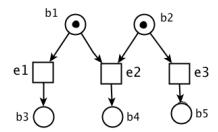
\includegraphics[scale = 0.7]{img/confu2.jpg}
      \caption{Esempio di confusione simmetrica tra $e_1$ ed $e_2$} 
    \end{figure}
  \end{enumerate}
  Petri era convinto, nella sua visione deterministica e senza conflitti, che
  l'avere una situazione di confusione nel modello fosse dovuto al non aver
  esplicitato alcuni aspetti o di aver costruito male il modello, con
  informazioni parziali e non complete sul modello e sull'ambiente.\\
  Un altro studioso, Einar Smith, molto vicino a Petri ha invece dimostrato come la
  confusione sia inevitabile
\end{definizione}
% \newpage
Vediamo un esempio famoso, detto della \textbf{mutua esclusione}, portato da
Smith per spiegare come la confusione sia inevitabile nella realtà.
\begin{esempio}
  Si analizza il seguente sistema:
  \begin{figure}[H]
    \centering
    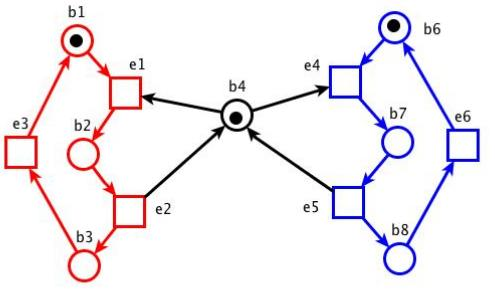
\includegraphics[scale = 0.4]{img/mes.jpg} 
  \end{figure}
  In rosso e in Blu abbiamo specificate le due componenti del sistema, che
  condividono una risorsa, ovvero la condizione $b_4$, che rappresenta che la
  risorsa è libera e a disposizione. L'evento $e_1$ e evento $e_4$ rappresentano
  eventi di acquisizione della risorsa (rispettivamente per la prima e per la
  seconda componente) e quindi le loro precondizioni rappresentano la necessità
  di acquisirla. Tra questi due eventi c'è una \textbf{situazione di
    conflitto}. Le condizioni $b_2$ e $b_7$, ovvero le rispettive postcondizioni
  dei due eventi, rappresentano che la risorsa è in uso per la rispettiva
  componente mentre gli eventi $e_2$ ed $e_5$ rappresentano il rilascio della
  risorsa condivisa, sempre per la rispettiva componente, arrivando
  rispettivamente nella componente $b_3$ e $b_8$. Ovviamente la risorsa
  non può essere contemporaneamente in uso da entrambe le risorse, quindi $b_2$
  e $b_7$ non possono essere contemporaneamente marcate, ovvero vere, e per
  questo si parla di \textit{mutua esclusione} (se una delle due è vera l'altra
  deve essere necessariamente falsa). D'altro canto gli
  eventi $e_3$ ed $e_6$ possono invece occorrere in modo concorrente senza
  conflitti.\\
  Scrivendo formalmente si ha che, nel caso che la risorsa sia stata acquisita
  dalla componente rossa e successivamente rilasciata:
  \[\{b_3,b_4,b_6\}[\{e_3,e_4\}>\{b_1,b_7\}\]
  ma se scatta prima $e_3$ ho il conflitto tra $e_1$ ed $e_4$, se scatta prima
  $e_4$ non ho conflitti con $e_1$. Quindi non ho informazioni sulla risoluzione
  del conflitto.\\
  \textbf{Capire se è confusione simmetrica}
\end{esempio}
\subsection{Sottoreti}
Partiamo subito con una definizione formale:
\begin{definizione}
  Siano $N=(B,E,F)$ e $N_1=(B_1,E_1,F_1)$ due reti elementari.\\
  Si dice che $N_1$ è \textbf{sottorete} di $N$ sse:
  \begin{itemize}
    \item $B_1\subseteq B$, quindi l'insieme delle condizioni della rete $N_1$
    è sottoinsieme di quello della rete $N$
    \item $E_1\subseteq E$, quindi l'insieme degli eventi della rete $N_1$
    è sottoinsieme di quello della rete $N$
    \item $F_1=F\cap[(B_1\times E_1)\cup (E_1\times B_1)]$, ovvero la relazione
    di flusso di $N_1$ è definita come la restrizione della relazione di flusso
    di $N$ rispetto alle condizioni e $B_1$ e agli eventi $E_1$ (tengo quindi solo
    gli archi di $N$ che connettono eventi e condizioni di $N_1$)
  \end{itemize}
\end{definizione}
\begin{definizione}
  Siano $N=(B,E,F)$ e $N_1=(B_1,E_1,F_1)$ due reti elementari.\\
  Si dice che $N_1$ è \textbf{sottorete generata da} $B_1$ di $N$ (ovvero di
  sottorete generata da un insieme di condizioni) sse:
  \begin{itemize}
    \item $B_1\subseteq B$, quindi l'insieme delle condizioni della rete $N_1$
    è sottoinsieme di quello della rete $N$
    \item $E_1=\, ^\bullet B_1\cup B_1^\bullet$, ovvero come eventi si
    hanno tutti quegli eventi che sono collegati in $N$ alle condizioni incluse
    nell'insieme di condizioni $B_1$, prendendo quindi tutti i pre-eventi e i
    post-eventi delle condizioni dell'insieme $B_1$
    \item $F_1=F\cap[(B_1\times E_1)\cup (E_1\times B_1)]$, ovvero la relazione
    di flusso di $N_1$ è definita come la restrizione della relazione di flusso
    di $N$ rispetto alle condizioni $B_1$ e agli eventi $E_1$
  \end{itemize}
  Non ho quindi una sottorete generata da un insieme arbitrario di condizioni ed
  eventi ma questi ultimi sono direttamente presi in relazione all'insieme delle
  condizioni scelto
\end{definizione}
\begin{definizione}
  Siano $N=(B,E,F)$ e $N_1=(B_1,E_1,F_1)$ due reti elementari.\\
  Si dice che $N_1$ è \textbf{sottorete generata da} $E_1$ di $N$ (ovvero di
  sottorete generata da un insieme di condizioni) sse:
  \begin{itemize}
    \item $B_1=\,^\bullet E_1\cup E_1^\bullet$, ovvero come condizioni si
    hanno tutte quelle condizioni che sono collegati in $N$ agli eventi inclusi
    nell'insieme di eventi $E_1$, prendendo quindi tutte e precondizioni e le
    postcondizioni degli eventi dell'insieme $E_1$
    \item $E_1\subseteq E$, quindi l'insieme degli eventi della rete $N_1$
    è sottoinsieme di quello della rete $N$
    \item $F_1=F\cap[(B_1\times E_1)\cup (E_1\times B_1)]$, ovvero la relazione
    di flusso di $N_1$ è definita come la restrizione della relazione di flusso
    di $N$ rispetto alle condizioni $B_1$ e agli eventi $E_1$
  \end{itemize}
  Non ho quindi una sottorete generata da un insieme arbitrario di condizioni ed
  eventi ma le prime sono direttamente prese in relazione all'insieme degli
  eventi scelto
\end{definizione}
\newpage
\begin{esempio}
  Tornando all'esempio della mutua esclusione:
  \begin{figure}[H]
    \centering
    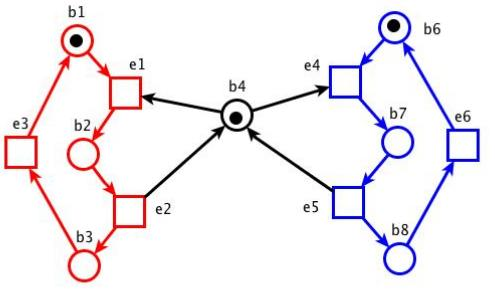
\includegraphics[scale = 0.4]{img/mes.jpg} 
  \end{figure}
  si ha, per esempio:
  \begin{itemize}
    \item in rosso si ha la sottorete $N'=(\{b_1,b_2,b_3\},
    \{e_1,e_2,e_3\},F')$, che è la sottorete generata  dall'insieme di
    condizioni $B'=\{b_1,b_2,b_3\}$ 
    \item in blu si ha la sottorete $N'=(\{b_6,b_7,b_8\},
    \{e_4,e_5,e_6\},F')$, che è la sottorete generata dall'insieme di condizioni
    $B'=\{b_6,b_7,b_8\}$
    \item si ha la sottorete $N'=(\{b_2,b_4,b_7\},\{e_1,e_2,e_4,e_5\},F')$, che
    è la sottorete generata  dall'insieme di condizioni $B'=\{b_2,b_4,b_7\}$
    \item si ha la sottorete $N'=(\{b_1,b_2,b_3,b_4\},\{e_1,e_2,e_3\},F')$, che è la
    sottorete generata da  dall'insieme di eventi $E'=\{e_1,e_2,e_3\}$
  \end{itemize}
\end{esempio}
\subsection{Operazioni di Composizione per Reti di Petri}
Data una rete $N=(B,E,F,c_0)$ questa può essere ottenuta componendo altre reti
di Petri. Si hanno in letteratura 3 modi principali:
\begin{enumerate}
  \item la \textbf{composizione sincrona}
  \item la \textbf{composizione asincrona}
  \item la \textbf{composizione mista, tra sincrona e asincrona}
\end{enumerate}
\newpage
Iniziamo informalmente a vedere degli esempi pratici.
\begin{esempio}
  Supponiamo di avere i modelli di due componenti, $N_1$, con un evento che
  corrisponde ad un'azione di invio, ed $N_2$, con un evento che corrisponde ad
  un'azione di ricezione:
  \begin{figure}[H]
    \centering
    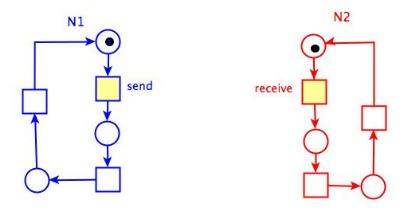
\includegraphics[scale = 0.5]{img/sinc.jpg} 
  \end{figure}
  Supponiamo che invio e ricezione siano eventi corrispondenti all'handshacking,
  ovvero l'invio avviene solo se può avvenire la ricezione.\\
  Vado quindi a sincronizzare questi due eventi, che diventano quindi un'unico
  evento nella rete composta, che è abilitato se le due precondizioni, nelle due
  componenti sono entrambe vere: 
  \begin{figure}[H]
    \centering
    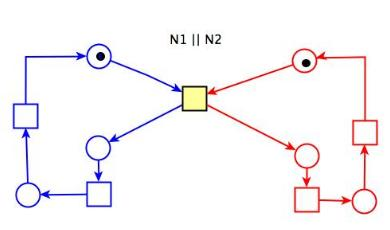
\includegraphics[scale = 0.5]{img/sinc2.jpg} 
  \end{figure}
  La composizione viene indicata con:
  \[N_1||N_2\]
  Lo scatto dell'evento, in maniera sincrona, rende vere le postcondizioni nelle
  due componenti e false le due precondizioni.\\
  Abbiamo appena visto un esempio di \textbf{composizione sincrona}
\end{esempio}
\newpage
\begin{esempio}
  Supponiamo di avere i modelli di due componenti, $N_1$, che invia in un canale
  un messaggio (per esempio in un buffer), e $N_2$, che riceverà il messaggio
  solo quando esso sarà disponibile:
  \begin{figure}[H]
    \centering
    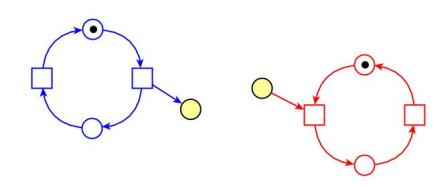
\includegraphics[scale = 0.5]{img/asinc.jpg} 
  \end{figure}
  In questo caso, a differenza dell'esempio precedente, non identifichiamo
  eventi ma condizioni. Identifico quindi il canale (le due condizioni) come uno
  solo, che avrà il pre-evento in una componente e il post-evento nell'altra.\\
  Quindi il pre-evento, nella componente $N_1$, può scattare solo se questa
  nuova condizione condivisa, il canale, è libera, indipendentemente dalla
  componente $N_2$. D'altro canto l'evento in $N_2$ può scattare solo se la
  condizione condivisa è marcata, indipendentemente dallo stato della prima
  componente, liberando il canale di comunicazione.\
  Avvio e ricezione (dopo che il messaggio è stato inviato può essere letto in
  un qualsiasi futuro) non sono sincronizzati e si ha quindi a che fare con
  un esempio di \textbf{composizione asincrona}
\end{esempio}
Sarà interessante studiare come la composizione di due componenti, per esempio,
senza deadlock non comporta, in generale, l'ottenimento di una rete priva di
deadlock.
\newpage
\section{Reti Posti e Transizioni}
Vediamo ora una nuova classe delle \textit{reti di Petri}, detta \textbf{reti
  Posti e Transizioni}, permette di rappresentare un sistema in modo più
compatto, sono una sorta di \textit{ripiegamento} dei sistemi
elementari. Partiamo quindi da un esempio:
\begin{esempio}
  prendiamo in studio sempre il sistema produttore-consumatore:
  Sia nella versione con contatto:
  \begin{figure}[H]
    \centering
    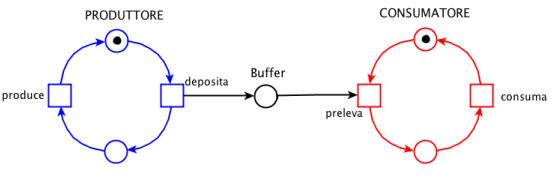
\includegraphics[scale = 0.5]{img/pt.jpg} 
  \end{figure}
  che senza:
  \begin{figure}[H]
    \centering
    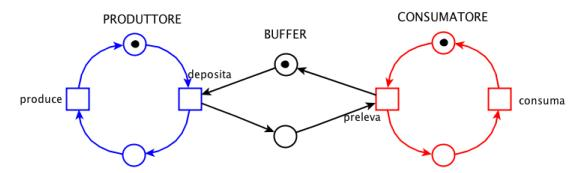
\includegraphics[scale = 0.5]{img/pt2.jpg} 
  \end{figure}
  Suppongo di voler modellare il sistema in modo che il buffer possa avere un
  numero determinato di posizioni, per esempio 2 (il buffer può quindi
  depositare fino a due elementi). Si ottiene quindi:
  \begin{figure}[H]
    \centering
    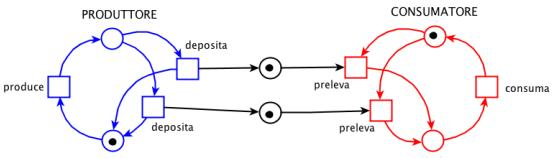
\includegraphics[scale = 0.6]{img/pt3.jpg} 
  \end{figure}
  Dove si hanno due posizioni del buffer (e quindi basta che una sia vuota per
  permettere al produttore di depositare) a disposizione del sistema. Si nota
  come l'aumento dei buffer complica drasticamente la modellazione del sistema.
  Si cerca quindi una soluzione più compatta, compattando gli eventi
  \textit{deposita} e \textit{preleva} e dando nuova notazione al buffer. Si
  ottiene:
  \begin{figure}[H]
    \centering
    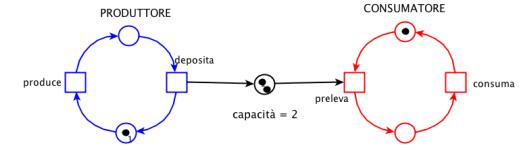
\includegraphics[scale = 0.6]{img/pt4.jpg} 
  \end{figure}
  con il buffer che diventa anche un \textbf{contatore} del numero di elementi
  presenti al suo interno. Un buffer a due posizioni diventa quindi una
  condizione non più booleana, detta \textbf{Posto}, con una \textbf{capacità}
  pari a 2. Il produttore non può produrre oltre la capacità.\\
  Con questa rappresentazione non ho più alcuna difficoltà nel rappresentare più
  posizioni del buffer in quanto basta aumentare la capacità. Ho però perso
  delle informazioni infatti non ho più una relazione di dipendenza tra dove si
  deposita (se nella prima posizione o nella seconda) e dove si preleva.\\
  Aggiungiamo un'altra complicanza: aggiungiamo un secondo consumatore:
  \begin{figure}[H]
    \centering
    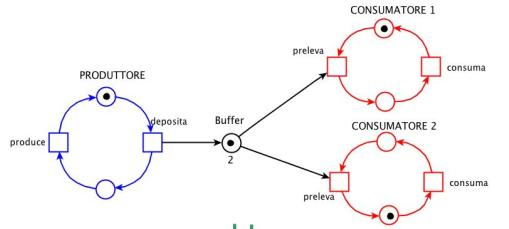
\includegraphics[scale = 0.6]{img/pt5.jpg} 
  \end{figure}
  Possiamo \textit{comprimere} nella stessa maniera, ottenendo, in quanto i due
  consumatori hanno lo stesso modello di comportamento:
  \begin{figure}[H]
    \centering
    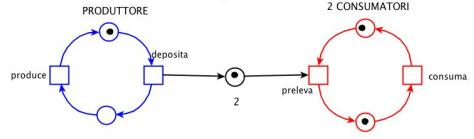
\includegraphics[scale = 0.7]{img/pt6.jpg} 
  \end{figure}
  Anche qui perdo l'informazione riguardo quale dei due consumatori ha
  effettivamente prelevato, riguardo quale dei due è pronto a \textit{prelevare}
  e quale a \textit{consumare}, continuando ad ignorare anche la posizione
  del buffer nei confronti della quale stanno agendo.\\
  Si può arrivare ad avere due componenti identiche che sono concorrenti tra
  loro. 
\end{esempio}
Le condizioni non sono più, in generale, booleane ma sono \textbf{posti}
dotati di \textbf{contatori}, gli elementi all'interno sono detti
\textbf{marche}. Ai posti si assegna anche una \textbf{capacità}. 
\\
Si ha inoltre che lo scatto di una transizione dipende dalla disponibilità
delle risorse, per esempio un produttore può produrre $n$ elementi alla volta
e il consumatore consumarne $m$. Si usano quindi archi pesati (se non indicato
ovviamente ha peso 1, quello del normale check booleano di condizione attiva)
tali che una transizione possa scattare sse i pesi vengono rispettati:
\begin{figure}[H]
  \centering
  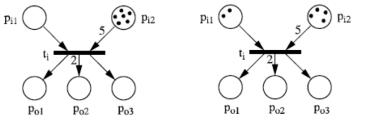
\includegraphics[scale = 0.7]{img/pt7.jpg}
  \caption{Esempi con la transizione $t_i$ non abilitata}
\end{figure}
\begin{figure}[H]
  \centering
  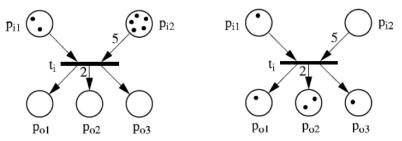
\includegraphics[scale = 0.7]{img/pt8.jpg}
  \caption{Esempio con la transizione $t_i$ abilitata, a sinistra il ``prima''
    e a destra il ``dopo'' lo scatto di $t_i$}
\end{figure}
\newpage
\begin{esempio}
  Petri aveva introdotto l'uso delle reti anche per le reazioni chimiche, per
  esempio:
  \begin{figure}[H]
    \centering
    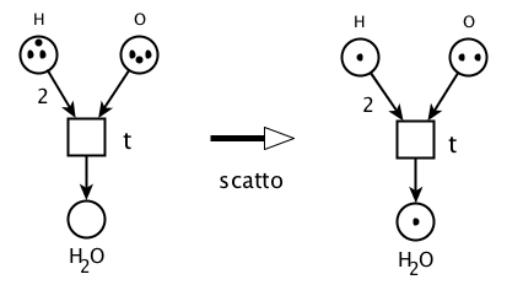
\includegraphics[scale = 0.35]{img/pt9.jpg}
    \caption{Esempio con la modellazione della produzione di $H_2O$}
  \end{figure}
\end{esempio}
\subsection{I Filosofi a Cena}
Questo è un classico problema di sincronizzazione, introdotto da Dijkstra. Si ha
un tavolo rotondo con 5 filosofi ($p_i,\,\i=0,\ldots 4$), ciascuno ha davanti un
piatto di spaghetti e si hanno solo 5 forchette ($f_i,\,\i=0,\ldots 4$):
\begin{figure}[H]
  \centering
  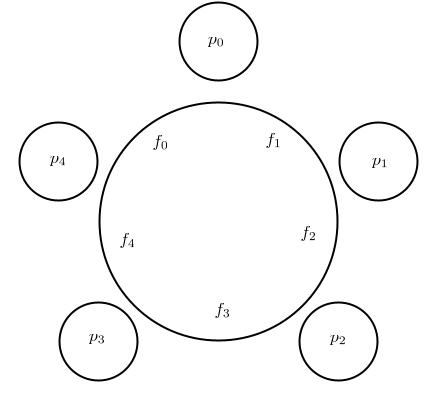
\includegraphics[scale = 0.5]{img/pt10.jpg}
  \caption{Rappresentazione schematica del problema dei 5 filosofi}
\end{figure}
Ogni filosofo ha lo stesso comportamento, un po' pensa e un po' mangia,
prendendo prima la forchetta alla sua destra e poi quella alla sua sinistra
(perché necessitano di due forchette per mangiare). Si ha quindi il
\textit{deadlock} se tutti vogliono mangiare, prendendo tutti in primis una
forchetta, impedendosi tutti a vicenda di mangiare (non potendo prendere due
forchette) o si ha la \textit{starvation} in quanto potrebbero accordarsi per
mangiare in quattro, impedendo a uno di mangiare.\\
Si vuole modellare tale schema. Ogni filosofo può essere modellato come una rete
elementare, che farà da componente al modello finale:
\begin{figure}[H]
  \centering
  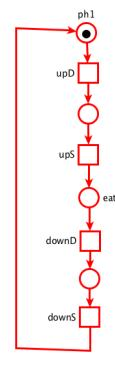
\includegraphics[scale = 0.5]{img/pt11.jpg}
\end{figure}
con gli eventi \textit{upD} e \textit{upS}, dove il filosofo prende la forchetta
destra e sinistra, e rispettivamente \textit{downD} e \textit{downS}, dove le
mette giù. Si ha la condizione che specifica che il filosofo sta pensando e
quella che mi segnala l'azione del mangiare, oltre alle due condizioni
intermedie che separano le azioni tra forchetta sinistra e destra.\\
Si modella anche la componente della forchetta, con gli eventi che segnalano se
è depositata, \textit{down}, o meno, \textit{up}:
\begin{figure}[H]
  \centering
  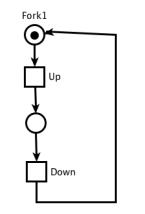
\includegraphics[scale = 0.5]{img/pt12.jpg}
\end{figure}
\newpage
Combino quindi le due componenti per specificare il filosofo che prende la sua
forchetta destra e poi la sinistra, quindi per ogni componente \textit{filosofo}
si hanno due componenti \textit{forchetta}:
\begin{figure}[H]
  \centering
  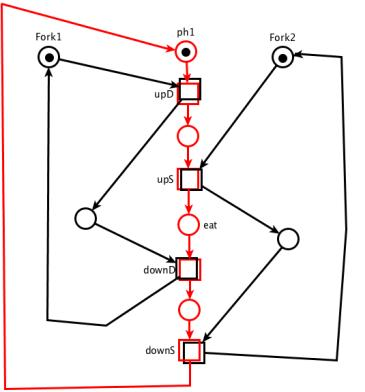
\includegraphics[scale = 0.5]{img/pt13.jpg}
\end{figure}
con la \textit{forchetta 1 (fork 1)} che sarà la forchetta destra e la
\textit{forchetta 2 (fork 2)} che sarà la forchetta sinistra. Si hanno quindi
diverse transizioni di sincronizzazione tra le due componenti (ogni volta che il
filosofo interagisce con la forchetta).\\
Bisogna aggiungere che ogni forchetta può essere presa da due filosofi, ognuna a
destra di un filosofo e a sinistra di un altro:
\begin{figure}[H]
  \centering
  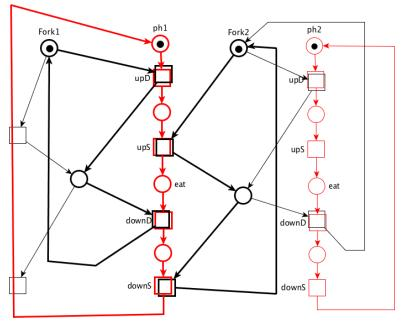
\includegraphics[scale = 0.5]{img/pt14.jpg}
\end{figure}
Ogni forchetta quindi si sincronizza alternativamente tra due filosofi, venendo
presa da uno dei due filosofi. Si è arrivati quindi ad una \textbf{situazione di
  conflitto}, o meglio ad una \textbf{situazione di confusione}.\\
Per ora la soluzione di questo problema viene lasciato da parte per valutare il
modello dello stesso.\\
Si ha quindi una possibile rappresentazione del modello completo:
\begin{figure}[H]
  \centering
  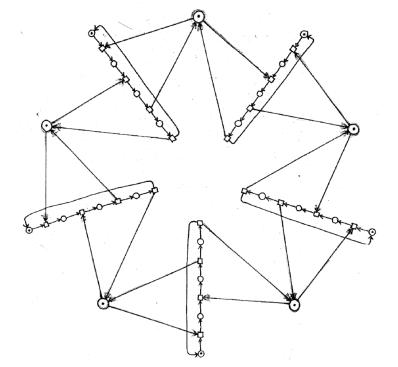
\includegraphics[scale = 0.5]{img/pt15.jpg}
\end{figure}
Ma ogni filosofo, come del resto ogni forchetta, si comporta nella stessa
maniera. Si tenda quindi di \textit{ripiegare} il modello, modellando un
un'unica componente filosofo con 5 marche distribuite nei vari stati locali del
filosofo. Stesso discorso per le forchette. Ottengo quindi il seguente modello:
\begin{figure}[H]
  \centering
  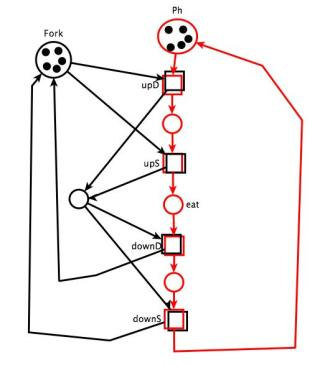
\includegraphics[scale = 0.6]{img/pt16.jpg}
\end{figure}
Con le due componenti, \textit{filosofo} e \textit{forchetta}, entrambe
inizializzate con 5 marche ciascuno. Questo modello però perde informazione
sulla forchetta che un filosofo può prendere, si ha un radicale \textbf{cambio
  di protocollo}. Un filosofo può prendere una qualsiasi forchetta e non più
quella alla sua destra/sinistra. Non posso quindi usare le \textit{reti Posti e
  Transizioni} in quanto perdo troppe informazioni.\\
L'unica soluzione possibile è quindi quella di recuperare le informazioni perse
inserendole nelle marche, alle quali viene aggiunta una struttura dati. Si ha
così modo di distinguere i vari filosofi e le forchette. Per compattare il
sistema devo quindi rendere più complessa l'essenza della marca, viene
arricchita con una struttura dati.\\
Si arriva così ad avere una \textbf{Rete di Alto Livello}, come, per esempio,
una \textit{rete colorata}, a partire da un rete elementare.\\
Distinguo quindi filosofi e forchette nei due insiemi di strutture dati:
\begin{enumerate}
  \item $Phil=\{p_0,\ldots, p_4\}$, insieme dei filosofi
  \item $Fork=\{f_0,\ldots, f_4\}$, insieme delle forchette
\end{enumerate}
Si nota che per gli indici si ha una somma \textit{modulo 5}, ovvero gli indici
rispondono alla regola:
\[(i+1) \mbox{ mod } 5\]
In modo che gli indici siano ordinati avendo inoltre lo 0 che segue il 4, in
modo circolare.\\
Si ottiene quindi, mantenendo il protocollo iniziale:
\begin{figure}[H]
  \centering
  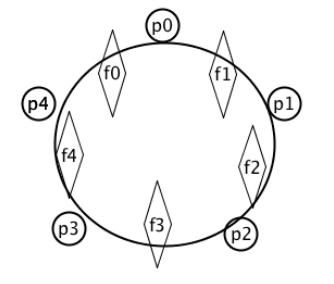
\includegraphics[scale = 0.6]{img/pt17.jpg}
\end{figure}
Si mantiene quindi un modello simile a quello descritto sopra ma al posto di
marche non strutturate si ha nel posto delle 5 forchette le marche dell'insieme
\textit{Fork} e al posto dei 5 filosofi le marche dell'insieme \textit{Phil}:
\begin{figure}[H]
  \centering
  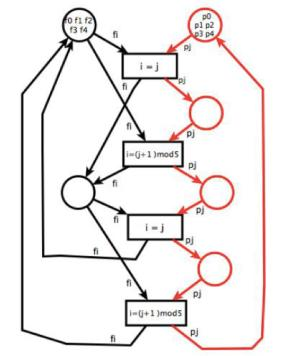
\includegraphics[scale = 0.6]{img/pt18.jpg}
\end{figure}
Le transizioni scattano in determinate condizioni. Per esempio la prima
transizione, relativa al fatto che il filosofo prende la forchetta alla sua
destra, scatta sse con l'istanza filosofo $p_j$ e forchetta $f_i$ si ha che
$i=j$ (ho quindi almeno una forchetta, almeno un filosofo e la forchetta deve
essere quella alla sua destra, che, per come abbiamo modellato il problema, è
quella con lo stesso indice). Sugli archi si hanno quindi annotate determinate
variabili che denotano istanze. Per la forchetta a sinistra si usa il modulo
5. Si procede quindi per i vari filosofi.
\begin{figure}[H]
  \centering
  \includegraphics[scale = 0.5]{img/pt19.jpg}
  \caption{Esempio con il filosofo $p_3$ che ha già preso la forchetta alla sua
    destra, $f_3$, e prende quella a sinistra, $f_4$}
\end{figure}
\textit{Si ha quindi un prezzo per rappresentare in maniera compatta un sistema
  elementare, mediante una rete di alto livello, ovvero l'arricchimento della
  struttura dati}.
\subsection{Formalizzazione delle Reti Posti e Transizioni}
Nonostante la sezione si occupi di formalismi ci appoggiamo ad un esempio per
avere un confronto diretto tra teoria e pratica. Questo esempio è un'n-sima
versione del sistema produttore-consumatore, con un produttore che deposita
a due elementi alla volta, in un buffer che ha capacità massima apri a cinque,
che vengono consumati da due consumatori:
\begin{figure}[H]
  \centering
  \includegraphics[scale = 0.65]{img/pt20.jpg}
\end{figure}
quindi al massimo ho cinque marche nel buffer e 2 in uno degli stati del
consumatore (in quanto rappresenta due consumatori).\\
Passiamo ora alla formalizzazione:
\begin{definizione}
  Si definisce un \textbf{sistema Posti e Transizioni (\textit{sistema P/T})} la
  sestupla: 
  \[\Sigma=(S,T,F,K,W;M_0)\]
  dove:
  \begin{itemize}
    \item $(S,T,F)$ è una rete con:
    \begin{itemize}
      \item $S$ che rappresenta l'insieme dei posti
      \item $T$ che rappresenta l'insieme delle transizioni
      \item $F$ che rappresenta la relazione di flusso che lega posti e
      transizioni tramite archi
    \end{itemize}
    \item $K:S\to\mathbb{N}^{+}\cup \{\infty\}$ che rappresenta una funzione che
    ad ogni posto in $S$ assegna un valore, che può essere un naturale
    strettamente positivo o anche infinito (ovvero in quel posto posso avere un
    numero qualsiasi di marche). Il valore zero non è ammesso in quanto
    implicherebbe che il posto non potrebbe mai essere occupato, rendendo la
    modellazione di un tale posto inutile. $K$ è detta \textbf{funzione
      capacità dei posti}.
    \item $W:F\to\mathbb{N}$ che rappresenta una funzione che
    assegna ad ogni arco un peso mediante un valore naturale che stavolta può
    essere, oltre che infinito, anche zero. $W$ è detta \textbf{funzione peso
      degli archi}
    \item $M_0:S\to \mathbb{N}\cup\{\infty\}:\,\forall s\in
    S\,\,t.c.\,\,M_0(s)\leq K(s)$ che rappresenta la \textbf{marcatura iniziale}
    del sistema, ovvero una funzione che assegna ad ogni posto un naturale,
    eventualmente nullo o infinito, minore o uguale alla capacità massima di
    tale posto (capacità espressa dalla funzione $K$) indicante il numero di
    marche allo stato iniziale. 
  \end{itemize}
  Bisogna ora definire la regola di scatto, ovvero il \textbf{gioco delle
    marche}, la regola per cui le marche si spostano sulla rete. Si ha quindi,
  dati:
  \[M:S\to\mathbb{N}\cup \{\infty\}\mbox{ e }t\in T\]
  ovvero data una marcatura e una qualsiasi transizione $t$ si ha che:
  \[M[t>\]
  ovvero una transizione è abilitata in una certa marcatura,
  \begin{center}
    sse:
  \end{center}
  \[\forall s\in S,\,\,M(s)\geq W(s,t)\wedge M(s)+W(t,s)\leq K(s)\]
  ovvero per ogni posto si ha che ci sono abbastanza marche nei posti perché
  possa scattare la transizione, ovvero c'è un arco di peso corretto che collega
  quel posto con la transizione, avendo peso dell'arco minore o uguale al numero
  di marche del posto, e, inoltre, si deve verificare che la transizione non
  metta troppe marche in quel posto, quindi la marcatura del posto (ovvero il
  numero di marche già presenti in esso) più il numero di marche che si
  aggiungono con lo scatto della transizione non deve superare la capacità del
  posto.
  \begin{figure}[H]
    \centering
    \includegraphics[scale = 0.75]{img/pt21.jpg}
    \caption{Nell'esempio si ha che la transizione $t_2$ può scattare sse nella
      posto precedente ho almeno due marche, in quanto l'arco tra i due ha peso
      due. Inoltre ho il posto che segue vuoto ma con capacità massima pari a
      tre, quindi la transizione può scattare in quanto l'arco tra i due pesa
      due, assicurandomi che dopo la transizione, nel posto che la segue, non
      verrà superata la capienza massima, arrivando infatti ad avere marcatura
      pari a 2}
  \end{figure}
  Lo scatto della transizione, se questa è abilitata nella marcatura, mi genera
  una nuova marcatura che viene ottenuta da quella precedente togliendo tante
  marche dal posto che è di input alla transizione quanto il peso dell'arco che
  connette tale posto alla transizione e aggiungendo tante marche al posto in
  output quante il peso dell'arco che connette la transizione a tale posto,
  ovvero, formalmente: 
  \[M[t>M'\]
  \begin{center}
    sse
  \end{center}
  \[M[t> \wedge\, \forall s\in S,\,\,M'(s)=M(s)-W(s,t)+W(t,s)\]
  quindi il nuovo posto avrà marcatura pari a quella precedente al più dei due
  contributi, il primo negativo e il secondo positivo, dei pesi dei due archi.
\end{definizione}
\begin{definizione}
  Dato un sistema P/T $\Sigma=(S, T , F , K , W;M_0)$ si definisce
  l'\textbf{insieme delle marcature raggiungibili}, dalla marcatura iniziale  di
  $\Sigma$ come:
  \[[M_0>\]
  ed esso è il più piccolo insieme tale che:
  \begin{itemize}
    \item $M_0\in [M_0>$, ovvero ola marcatura iniziale appartiene all'insieme
    delle marcature raggiungibili
    \item se $M\in [M_0> \wedge\,\exists t\in T:\,M[t>M'$ allora $M'\in [M_0$,
    ovvero se $M$ appartiene all'insieme delle marcature raggiungibili ed esiste
    una transizione una transizione tale per cui $M$ va in $M'$ allora, di
    conseguenza si ha che $M'$ appartiene all'insieme delle marcature
    raggiungibili dallo stato iniziale
  \end{itemize}
  \emph{Anche questa è una definizione per induzione}
\end{definizione}
\begin{esempio}
  Vediamo qualche esempio particolare (se la capacità non è specificata si ha
  che essa è infinita):
  \begin{figure}[H]
    \centering
    \includegraphics[scale = 0.5]{img/pt22.jpg}
    \caption{Lo scatto toglie due marche dall'input e ne mette una nell'output
      ma la seconda volta $t$ non sarebbe più abilitata in quanto il posto in
      output si satura alla prima transizione, è un caso di \textbf{contatto}}
  \end{figure}
  \begin{figure}[H]
    \centering
    \includegraphics[scale = 0.5]{img/pt23.jpg}
    \caption{La transizione $t$ è abilitata avendo i posti in ingresso col
      giusto numero di marche e in uscita ha un posto vuoto che può riempire a
      piacere e lo stesso porto che prima aveva in input che può riempire con
      una marca rispettando le regole di capacità}
  \end{figure}
  \begin{figure}[H]
    \centering
    \includegraphics[scale = 0.5]{img/pt24.jpg}
    \caption{La transizione $t$ non è abilitata, e non lo sarà mai in $M$ in
      quanto la regola di scatto prevede che ci sia a priori una capacità
      sufficiente nei posti di output, cosa che qui non accade avendo uno di
      essi capacità uno, non si ragiona in modo sequenziale ``prima tolgo e poi
      metto'', lo spazio deve essere disponibile a priori per far scattare la
      transizione} 
  \end{figure}
  \newpage
  \begin{figure}[H]
    \centering
    \includegraphics[scale = 0.6]{img/pt25.jpg}
    \caption{In questa rete si ha che $t_1$ e $t_2$ sono abilitate in $M$ ed
      esse sono \textbf{concorrenti} in quanto lo scatto dell'una non disabilita
      lo scatto dell'altra dovendo entrambe prelevare una marca da un posto che
      ne contiene due per riversarne una ciascuna in un posto libero. Si ha
      quindi concorrenza anche in corrispondenza di transizioni non
      indipendenti}  
  \end{figure}
  \begin{figure}[H]
    \centering
    \includegraphics[scale = 0.55]{img/pt26.jpg}
    \caption{In questa rete si ha che $t_1$ e $t_2$ sono in \textbf{conflitto} e
      \textbf{non concorrenti} tra loro. Si ha infatti che lo scatto di una
      disabilita quella dell'altra, visto che da sola $t_2$ svuoterebbe il posto
      in input (se scatta prima $t_1$ poi ho una sola marca nello stato in input
      disabilitando $t_2$ che ne richiede due, viceversa lo scatto di $t_2$
      lascerebbe vuoto lo stato in input impedendo a $t_1$ di scattare). Il
      conflitto è dato non dalla struttura della rete ma dalla sua marcatura
      iniziale. Quindi in questa rete con questa marcatura può scattare una sola
      delle due transizioni, inoltre $t_1$ potrebbe occorrere due volte senza
      errori, essendo quindi, se occorre contemporaneamente per quelle due volte,
      \textbf{concorrente con se stessa}. La doppia occorrenza di $t_1$, indicatat
      con $2t_1$ è un \textbf{passo}}  
  \end{figure}
  \begin{figure}[H]
    \centering
    \includegraphics[scale = 0.5]{img/pt27.jpg}
    \caption{In questa rete si ha che $t_1$ è abilitata due volte, avendo
      quindi $2t_1$ e lo è anche $t_2$, che può scattare solo una volta. Si ha
      quindi che $t_1$ occorre concorrente con se stessa e contemporaneamente
      concorrente con $t_2$. Si ha quindi che il \emph{multiset} $2t_1+t_2$ è un
      \textbf{passo abilitato}} 
  \end{figure}
\end{esempio}
Si da ora la definizione formale di \textit{multiset di transizioni abilitate}
in un sistema:
\begin{definizione}
  Dato un sistema P/T $\Sigma=(S, T , F , K , W;M_0)$ si definisce un
  \textbf{multiset} $U:T\to\mathbb{N}$ come una funzione che assegna ad una
  transizione un numero naturale. Si ha inoltre che:
  \begin{itemize}
    \item un multiset è detto \textbf{concorrentemente abilitato} in
    $M\in[M_0>$, quindi con $M$ marcatura raggiungibile. Detto in maniera
    diversa $U$ è un passo $M[U>$. Un multiset è concorrentemente abilitato in
    $M$ sse:
    \[\forall s\in S,\,\,\sum_{t\in T}U(t)\cdot W(s,t)\leq M(s)\,\,\wedge\,\,
      M(s)+\sum_{t\in T}U(t)\cdot W(t,s)\leq K\]
    ovvero per ogni posto si devono avere un numero di marche nella marcatura
    iniziale superiore al numero che posso togliere mediante le varie
    transizioni nel multiset $U$. Inoltre le marche che devo aggiungere più il
    numero di marche già presenti nel posto in output deve essere inferiore alla
    capacità dell'output.\\
    Questa condizione può essere riscritta come:
    \[\sum_{t\in T}U(t)\cdot W(s,t)\leq M(s)\leq K(s)-\sum_{t\in T}U(t)\cdot
      W(t,s)\]
    \item un multiset $U$ abilitato in $M$ può occorrere generando $M'$, avendo
    quindi:
    \[M[U>M'\]
    sse:
    \[\forall s\in S\,\,M'(s)=M(s)-\sum_{t\in T}U(t)\cdot W(s,t)+\sum_{t\in
        T}U(t)\cdot W(t,s)\]
    quindi la marcatura $M'$ in un certo posto è uguale alla marcatura del posto
    presente prima del passo al più dei contributi, positivi e negativi, delle
    varie transizioni (positivi se si ha tale posto come output e negativi se lo
    si ha come input)
    \item $U_\Sigma$ è l'\textbf{insieme dei passi} di $\Sigma$ e viene definito
    come:
    \[U_\Sigma=\{U:T\to \mathbb{N}|\,\,\exists M,M'\in [M_0>:\,\,M[U>M'\}\]
    ovvero l'insieme dei passi possibili tali per cui passo da una marcatura
    raggiungibile ad un'altra attivando il passo
  \end{itemize}
\end{definizione}
\begin{definizione}
  Dato un sistema P/T $\Sigma=(S, T , F , K , W;M_0)$ si definisce il
  \textbf{grafo di raggiungibilità}, indicato con
  $RG(\Sigma)$, costruito solo con posti di capacità finita in quanto avere
  capacità infinite comporterebbe avere un grafo infinito, come la quadrupla:
  \[RG(\Sigma)=([M_0 >, U_\Sigma , A, M_0 )\]
  dove, per rappresentare questo sistema di transizioni, si ha:
  \begin{itemize}
    \item $[M_0>$ che rappresenta le marcature raggiungibili dallo stato iniziale
    del sistema $\Sigma$. Sono così rappresentati gli stati del sistema di
    transizioni  
    \item $U_\Sigma$ rappresenta l'insieme dei passi che rappresenta l'alfabeto
    delle etichette degli archi
    del sistema di transizioni
    \item $A=\{(M,U,M'):\,M,M'\in [M_0>\,\wedge\, U\in U_\Sigma \,\wedge\,
    M[U>M'\}$ dove, quindi dalla marcatura $M$ ho un arco, etichettato $U$, alla
    marcatura $M'$ sse le due marcature sono raggiungibili dallo stato iniziale,
    ed esiste un passo, nell'insieme dei passi, abilitato in $M$ tale per cui
    posso passare dalla marcatura $M$ alla marcatura $M'$. È quindi la regola
    che definisce come connettere mediante archi i vari stati
    \item $M_0$ che rappresenta la marcatura iniziale del sistema nonché lo
    stato iniziale del sistema di transizioni
  \end{itemize}
  Se $U$ è una singola transizione si ha il grafo di raggiungibilità
  sequenziale, detto $SGR(\Sigma)$.\\
  \textbf{La diamond property non è più valida in questa classe di reti a causa
    dei \emph{self loop} che posso avere tra una transizione e un posto}
\end{definizione}
\begin{esempio}
  Si prenda il sistema P/T $\Sigma$:
  \begin{figure}[H]
    \centering
    \includegraphics[scale = 0.7]{img/pt31.jpg} 
  \end{figure}
  \newpage
  Si ha che lo scatto di $t_1$ e lo scatto di $t_2$ non può essere contemporaneo
  in quanto si richiederebbero due marche nel posto $s$, devono quindi scattare
  in sequenza. SI ottiene che il grafo dei casi raggiungibili è uguale a quello
  dei casi raggiungibili sequenziale e quindi non vale la diamond property (non
  potendo aggiungere alcun arco tra $\{s_1,s,s_2\}$ e $\{s\}$):
  \begin{figure}[H]
    \centering
    \includegraphics[scale = 0.7]{img/pt32.jpg}
  \end{figure}
\end{esempio}
\begin{definizione}
  Dato un sistema P/T si ha che una transizione $t$ è in una \textbf{situazione
    di contatto} nella marcatura $M$ sse:
  \[\forall s\in S, W(s,t)\leq M(s)\,\wedge\,\exists\, s\in S:\,
    M(s)+W(t,s)>K(s)\] 
  
  ovvero una transizione  in una situazione di contatto se tutti i suoi
  pre-posti hanno abbastanza marche e almeno uno dei suoi post-posti ne ha
  troppe per permettere il suo scatto. Formalmente si ha che l'arco tra il posto
  in input e la transizioni ha peso inferiore al numero di marche dell'input e
  la marcatura del posto output più le marche che vengono aggiunte è maggiore
  della capacità del posto di output stesso.\\
  Un esempio:
  \begin{figure}[H]
    \centering
    \includegraphics[scale = 0.65]{img/pt33.jpg}
    \caption{Esempio di situazione di contatto}
  \end{figure}
\end{definizione}
\newpage
Si cerca di capire se è possibile trasformare la rete da una con contatti ad una
senza modificarne il comportamento. Questo è possibile con la
\textbf{complementazione}. Preso un posto $s$ se ne fa il complemento
$\overline{s}$, ovvero si fa un altro posto che ha archi in output verso
transizioni che sono di input a quelle del posto considerato e viceversa per gli
archi in input. Il complemento è quindi collegato alle stesse transizioni del
posto considerato ma con archi direzionati all'inverso. Per quanto riguarda il
numero di marche del complemento bisogna avere che il numero di marche del posto
e del suo complemento siano di somma pari alla capacità del posto (che è pari a
quella del complemento), ovvero:
\[M_0(\overline{s})=K(s)-M_0(s)\]
Si può inoltre dimostrare che per ogni marcatura raggiungibile $M$ la somma
delle marcature tra un posto e il suo complemento è sempre la medesima, comunque
evolva il sistema:
\[M(\overline{s})+M(s)=K(s)\]
\begin{figure}[H]
  \centering
  \includegraphics[scale = 0.65]{img/pt35.jpg}
\end{figure}
\begin{definizione}
  Dato un sistema P/T $\Sigma=(S, T , F , K , W;M_0)$ è \textbf{senza contatti}
  sse:
  \[\forall M\in[M_0>,\,\forall t\in T,\forall s\in S\]
  si ha:
  \[M(s)\geq W(s,t)\Rightarrow M(s)+W(t,s)\leq K(s)\]
  ovvero ogni volta che ho abbastanza marche in un posto di input ad una
  transizione allora sicuramente non ne ho troppe nel posto di output
\end{definizione}
\begin{definizione}
  Dato un sistema P/T $\Sigma=(S, T , F , K , W;M_0)$ senza contatti allora si
  ha che una transizione $t\in T$ è abilitata in $M\in[M_0>$, che si indica
  con $M[t>$, sse: 
  \[\forall s\in S,\,\,M(s)\geq W(s,t)\]
  ovvero sse nei posti in input ho abbastanza marche (trascurando di studiare
  i posti in output essendo una rete senza contatti).\\
  Si ha quindi che in assenza di contatti la capacità dei posti non gioca più
  alcun ruolo nella regola di scatto in quanto controllo solo di avere
  sufficienti marche in input per far scattare una transizione
\end{definizione}
\subsection{Reti Marcate}
Si cerca di identificare i sistemi elementari come casi particolari dei sistemi
P/T.
\begin{definizione}
  Dato un sistema P/T $\Sigma=(S, T , F , K , W;M_0)$ si ha che $\Sigma$ è una
  \textbf{Rete Marcata} sse:
  \[\forall s\in S,\,\,M_0(s)\in\mathbb{N}\,\wedge \,K(s)=\infty
    \,\wedge\,\forall t\in T,\,\,W(s,t)\leq 1\,\wedge\, W(t,s)\leq 1 \]
  ovvero per ogni posto la marcatura iniziale assegna un valore finito al posto
  che però ha capacità infinita (che quindi non gioca nessun ruolo, non
  vincolando lo scatto della transizione). Inoltre il peso di ogni arco deve
  essere minore o uguale a uno, imponendo quindi che abbia o peso uno o peso
  nullo (che segnala l'assenza dell'arco).\\
  Questa sottoclasse delle reti P/T può essere denotata con la sola quadrupla:
  \[\Sigma=(S,T,F;M_0)\]
  in quanto la capacità, denotata dalla funzione $K$, e il peso degli archi,
  denotato dalla funzione $W$, diventano ridondanti ed eliminabili dallo studio
  della rete.
\end{definizione}
\begin{definizione}
  Una rete marcata è definita \textbf{safe (sicura)} sse per ogni marcatura
  raggiungibile, compresa quella iniziale, ogni posto contiene al massimo una
  marca (tornando quindi ad una definizione simil booleana dello stato del posto
  che o è vuoto o contiene una marca). Formalmente si ha che una rete marcata è
  safe sse: 
  \[\forall M\in[M_0>,\,\forall s\in S:\,\,M(s)\leq 1\]
  \textbf{In una rete marcata i self-loop possono essere abilitati}:
  \begin{figure}[H]
    \centering
    \includegraphics[scale = 0.75]{img/pt36.jpg}
    \caption{Esempio di loop (o cappio) su una rete marcata}
  \end{figure}
  Si ricorda che in una rete elementare in ogni caso il self-loop non è
  abilitato e questa è una delle differenze principale tra un sistema elementare
  e una rete marcata, differenza alle quali si aggiungono anche il fatto che in
  una rete marcata ho capacità infinita e non pari a uno e marcature di un posto
  intere e non booleane. Sia nei sistemi elementari che nelle reti marcate ho
  solo archi di peso 1. \\
  Si ha di conseguenza che un \emph{sistema elementare puro}, ovvero un sistema
  elementare che non presenta mai cappi, \emph{coincide}, $\cong$, con una
  \emph{rete marcata pura e safe}, quindi senza cappi e con al più una marca per
  posto (quindi o una marca o zero marche).
  \\
  \textit{Poter vedere un sistema elementare come sottoclasse delle reti P/T
    permette varie possibilità dal punto di vista pratico.}
\end{definizione}
\subsection{Proprietà di Comportamento}
Si considerano sistemi P/T del tipo $\Sigma=(S,T,F,K,W;M_0)$ tali che $\forall
s\in S$ si ha $K(s)=\infty$ quindi con capacità dei posti illimitata.
\begin{figure}[H]
  \centering
  \includegraphics[scale = 0.35]{img/ptc.jpg}
  \caption{Esempio di sistema P/T}
\end{figure}
Abbiamo già visto la teoria dietro il grafo di raggiungibilità ma a questa vanno
aggiunte le tecniche di rappresentazione. La differenza con i grafi di sistemi
elementari si ritrova nel fatto che le marcature possono essere rappresentate da
un vettore colonna, con tanti elementi quanti i posti della rete, contenente
nell'i-sima posizione il numero di marche dell'i-simo posto in una data 
marcatura.\\
Solitamente il grafo di raggiungibilità viene usato per indagare le proprietà di
comportamento.
\begin{figure}[H]
  \centering
  \includegraphics[scale = 0.65]{img/ptc2.jpg}
  \caption{Grafo di raggiungibilità del sistema precedente, si nota, per
    esempio, che con $(0,1,2)$ si indica che in quello stato
    $M(s_1)=0$,$M(s_2)=1$ e $M(s_3)=2$ } 
\end{figure}
\subsubsection{Limitatezza}
Vediamo innanzitutto un problema famoso, detto \textbf{problema di
  raggiungibilità}.\\
In tale problema si ha una rete e due marcature, $M$ e $M'$, e ci si domanda se
dalla prima marcatura, raggiungibile dalla marcatura iniziale $M_0$, si può
raggiungere la seconda. Formalmente si ha che:
\[RP= \{\langle(S, T , F , W ), M, M'\rangle | (S, T , F , W ) \mbox{ è una rete
    P/T},\,M,M':S\to \mathbb{N} \mbox{ e } M'\in[M>\}\]
Questo problema è stato dimostrato decidibile da Mayr, anche se esponenziale
nello spazio. È un problema hard.\\
Si ha quindi l'importanza del fatto che il grafo delle marcature sia limitato e
viene quindi studiato il \textbf{problema della limitatezza}.
\begin{definizione}
  Sia $\Sigma=(S,T,F,K,W;M_0)$ un sistema P/T con $K(s)=\infty,\forall s\in
  S$. Sia inoltre definito $n\in\mathbb{N},\,\,n\geq 1$. Si ha quindi che il
  sistema in analisi è:
  \begin{itemize}
    \item \textit{\textbf{n-bounded} (n-limitato)} sse $\forall s\in S$ e
    $\forall M\in 
    M_0[>$ si ha:
    \[M(s)\leq n\]
    ovvero sse per ogni posto e per ogni marcatura raggiungibile da quella
    iniziale non succede che su tale posto si accumulino più di $n$ marche
    \begin{figure}[H]
      \centering
      \includegraphics[scale = 0.55]{img/ptc4.jpg}
      \caption{Esempio di sistema \emph{2-bounded} (ma non 1-bounded)}
    \end{figure}
    \item \textit{\textbf{bounded} (limitato)} sse $\exists n\in\mathbb{N}$ tale
    per cui $\forall s\in S$ e $\forall M\in M_0[>$ si ha:
    \[M(s)\leq n\]
    ovvero se esiste un limite per il numero di marche
    \begin{figure}[H]
      \centering
      \includegraphics[scale = 0.55]{img/ptc5.jpg}
      \caption{Esempio di sistema \emph{non bounded}, si andrà in
        \emph{overflow}} 
    \end{figure}
    Si ha di conseguenza una proposizione:
    se $\Sigma$ è \textbf{limitato} allora il numero delle marcature
    raggiungibili dalla marcatura iniziale è un insieme \textbf{finito}, ovvero
    $[M_0>$ è un insieme finito, e quindi il grafo di raggiungibilità (il grafo
    delle marcature) è finito sia nel caso sia standard che in quello sia
    sequenziale: 
    \begin{itemize}
      \item $SG(\Sigma)$ è finito
      \item $SGR(\Sigma)$ è finito
    \end{itemize}
    \item \textit{\textbf{safe} (1-safe, sicuro)} sse $\forall s\in S$ e
    $\forall M\in 
    M_0[>$ si ha:
    \[M(s)\leq 1\]
    ovvero ho al più una marca per posto comunque evolva il sistema  
    \begin{figure}[H]
      \centering
      \includegraphics[scale = 0.55]{img/ptc3.jpg}
      \caption{Esempio di sistema \emph{safe} (ovvero 1-bounded)}
    \end{figure}
    Un sistema safe con $n$ posti ha al più $2^n$ marcature raggiungibili
  \end{itemize}
\end{definizione}
\subsubsection{Terminazione}
Un'altra proprietà interessante è quella della \textbf{terminazione}, in quanto
è spesso necessario che un sistema sequenziale termini (a differenza di uno
concorrente che spesso non ha termine).
\begin{definizione}
  Sia $\Sigma=(S,T,F,K,W;M_0)$ un sistema P/T. Si ha che:
  \begin{itemize}
    \item $\Sigma$ è detto \textbf{terminante} sse non ammette sequenze
    infinite.\\
    Inoltre $M\in[M_0>$ è una \textbf{marcatura di deadlock} sse $\forall t\in
    T$ non si ha $M[t>$, ovvero una marcatura in cui non è abilitata alcuna
    transizione. \\
    Ne segue che un sistema è terminante se arriva in una marcatura di
    deadlock.\\
    \item $\Sigma$ è \textbf{deadlock-free} sse $\forall M\in[M_0>$:
    \[\exists t\in T:\,\, M[t>\]
    ovvero sse non esiste una marcatura di deadlock raggiungibile da quella
    iniziale. Scritto diversamente:
    \[\nexists M\in[M_0>:\,\,M\mbox{ è una marcatura di deadlock}\]
    \item $\Sigma$ è \textit{\textbf{1-live} (1-vivo)} sse $\forall t\in T$:
    \[\exists M\in [M_0>:\,\,M[t>\]
    ovvero sse ogni transizione può essere abilitata almeno una volta (ho sempre
    una marcatura raggiungibile che abilita una transizione).\\
    \textit{Non avere un sistema 1-live implica un errore nella modellazione
      dello stesso in quanto si ha una transizione mai abilitata superflua}
    \item $\Sigma$ è \textit{\textbf{live} (vivo)} sse $\forall t\in T$ e
    $\forall M\in[M_0>$:
    \[\exists M'\in[M>:\,\,M'[t>\]
    ovvero sse per ogni transizione e per ogni marcatura raggiungibile esiste
    sempre un'altra marcatura raggiungibile che abilita la transizione.\\
    \textit{Si ha che un sistema \emph{live} comporta che tale sistema sia anche
      \emph{deadlock-free} mentre il fatto che un sistema sia
      \emph{deadlock-free} non implica necessariamente che sia anche
      \emph{live}} 
  \end{itemize}
\end{definizione}
\newpage
\begin{esempio}
  Vediamo qualche esempio:
  \begin{figure}[H]
    \centering
    \includegraphics[scale = 0.55]{img/ptc6.jpg}
    \caption{Esempio di sistema \emph{terminante} (quindi non deadlock-free), in
      quanto scatta al più due volte}
    \includegraphics[scale = 0.55]{img/ptc7.jpg}
    \caption{Esempio di sistema \emph{deadlock-free}, \emph{non terminante} e
      \emph{1-live} ma non live, in quanto può continuare a cicalare, ogni
      transizione scatta almeno una volta ma la prima può scattare solo una
      volta e non può più essere attivata} 
    \includegraphics[scale = 0.55]{img/ptc8.jpg}
    \caption{Esempio di sistema \textit{live}, \emph{non terminante} e
      \emph{deadlock-free}, in quanto si ha un ciclo infinito lungo tutto il
      sistema} 
    \includegraphics[scale = 0.55]{img/ptc9.jpg}
    \caption{Esempio di sistema \emph{1-live} ma non \emph{live}, \emph{non
        terminante} e \emph{non deadlock-free}, in quanto potrebbe sia terminare
      che non terminare non potendo permettere la riattivazione di tutte le
      transizioni}  
  \end{figure}
\end{esempio}
\newpage
\subsubsection{Reversibilità}
Un'altra proprietà di comportamento è quella della \textbf{reversibilità}, detta
anche della \textbf{ciclicità}
\begin{definizione}
  Sia $\Sigma=(S,T,F,K,W;M_0)$ un sistema P/T. Si ha che $\Sigma$ è
  \textit{\textbf{reversible} (\textit{reversibile})} sse:
  \[\forall M\in[M_0>:\,\,M_0\in[M>\]
  ovvero se da una marcatura raggiungile da quella iniziale posso tornare alla
  marcatura iniziale stessa.\\
  \begin{figure}[H]
    \includegraphics[scale = 0.55]{img/ptc10.jpg}
    ~
    \includegraphics[scale = 0.55]{img/ptc1.jpg}
    \caption{A sinistra un esempio di sistema \emph{reversible} e a destra uno
      \emph{non reversible}} 
  \end{figure}
  \textit{Si ha che avere un sistema \emph{reversible} e \emph{1-live} implica
    avere un sistema \emph{live} ma non si ha per forza il contrario}
\end{definizione}
\subsubsection{Tecniche di Verifica delle Proprietà}
La prima tecnica usata per studiare le proprietà sopra descritte è quello
dell'analisi del grafo di raggiungibilità $RG(\Sigma)$ e di quello di
raggiungibilità sequenziale $(SGR(\Sigma))$.\\
Si ha innanzitutto che:
\textit{Se $RG(\Sigma)$ è\textbf{ finito}, allora esistono algoritmi per
  decidere le seguenti proprietà:}
\begin{itemize}
  \item un posto è \textit{safe, m-bounded, bounded}
  \item il sistema $\Sigma$ è \textit{safe, n-bounded, limitato}
  \item una transizione è \textit{\textbf{dead} (morta)},
  \textit{1-live},\textit{ live} (\textit{live} se per ogni marcatura
  raggiungibile ho un cammino che contiene tale transizione)
  \item il sistema $\Sigma$ va in \textit{deadlock}, è \textit{deadlock-free,
    1-live e live} 
  \item il sistema $\Sigma$ è \textit{reversible}
\end{itemize}
\newpage
Si hanno quindi due risultati interessati:
\begin{enumerate}
  \item \textit{un sistema $\Sigma$ \textbf{terminante}, ovvero che va in
    \textbf{deadlock}, implica che il grafo di raggiungibilità $RG(\Sigma)$ ha
    almeno un \textbf{nodo terminante}, ovvero un nodo da cui non escono archi,
    e viceversa}.
  \begin{figure}[H]
    \centering
    \includegraphics[scale = 0.6]{img/ptc12a.jpg}
    \includegraphics[scale = 0.6]{img/ptc12b.jpg}
    \caption{Esempio di un sistema terminante, col suo grafo di raggiungibilità
      che presenta, appunto, un nodo terminante, il nodo etichettato con
      ``$0100$''}
  \end{figure}
  \item \textit{un sistema $\Sigma$ \textbf{reversible} implica che il grafo di
    raggiungibilità $RG(\Sigma)$, come del resto anche quello sequenziale
    $SRG(\Sigma)$, è \textbf{fortemente connesso}, e viceversa}.\\
  Si ricorda che un grafo orientato è fortemente connesso se per ogni coppia di
  nodi esiste un cammino orientato dal primo al secondo nodo.
  \begin{figure}[H]
    \centering
    \includegraphics[scale = 0.7]{img/ptc13.jpg}
    \includegraphics[scale = 0.7]{img/ptc14.jpg}
    \caption{Esempio di sistema \emph{live}, \emph{1-safe} e \emph{non
        reversible} con il grafo di raggiungibilità, quindi, \emph{non
        fortemente connesso}} 
  \end{figure}
\end{enumerate}
\newpage
Oltre allo studio del grafo di raggiungibilità si hanno altre tecniche di
verifica delle proprietà, tra cui l'\textbf{analisi strutturale del grafo della
  rete} che sfrutta: 
\begin{itemize}
  \item \textbf{tecniche di algebra lineare}, che sfruttano la rappresentazione
  algebrica della rete, mediante:
  \begin{itemize}
    \item \textit{equazioni di stato} che descrivono la dinamica attraverso
    operazioni algebriche tra matrici
    \item \textit{S-invarianti} e \textit{T-invarianti}
  \end{itemize}
  \item \textbf{studio del grafo della rete, di particolari sottoinsiemi di
    nodi e altre caratteristiche}
  \item \textbf{condizioni necessarie e sufficienti per garantire proprietà di
    comportamento di particolari sottoclassi di reti} 
\end{itemize}
\subsubsection{Safety, Liveness e Fairness}
Le proprietà che specificano il comportamento dei \textbf{sistemi concorrenti
  e/o distribuiti} (detti anche \textbf{reattivi}) sono classificate in tre
principali categorie, a seconda del tipo di comportamento che descrivono:
\begin{enumerate}
  \item \textbf{proprietà di safety}, che descrivono proprietà che non devono
  mai accadere, dichiarano che ``mai accadranno comportamenti indesiderati''
  (ad esempio: mai un semaforo avrà accese contemporaneamente le luci
  verde e rossa; mai due semafori ad un incrocio saranno contemporaneamente
  verdi). \\\textit{Nota: questa proprietà non ha nulla a che vedere con la
    \emph{1-safeness} (la \emph{safeness}) delle reti P/T}
  \item \textbf{proprietà di liveness}, che descrivono proprietà che devono
  essere verificate da tutte le esecuzioni, dichiarano che ``prima o poi un
  certo fatto deve accadere'' (ad esempio, prima o poi il semaforo diventa
  verde) 
  \item \textbf{proprietà di fairness}, che descrivono proprietà che
  ``descrivono fatti che devono accadere infinitamente spesso'' (ad esempio, la
  luce verde si accende infinitamente spesso)
\end{enumerate}
\subsection{Analisi Strutturale}
Spesso studiare il grafo di raggiungibilità comporta un costo esponenziale nel
numero dei posti della rete, le marcature sono almeno dell'ordine di
$2^{posti}$. Si passa quindi dallo studio del grafo di raggiungibilità allo
studio della rete stessa mediante la cosiddetta \textbf{analisi strutturale},
che studia il \textbf{grafo della rete}
\begin{definizione}
  Sia $\Sigma=(S,T,F;M_0)$ una \textbf{rete marcata}, reti con capacità
  dei posti illimitata e peso degli archi $\leq$ 1 (quindi o 0 o 1). Possiamo
  quindi studiare alcune proprietà strutturali che danno indicazioni sulle
  proprietà di comportamento:
  \begin{itemize}
    \item se un sistema $\Sigma$ è \emph{safe} e \emph{bounded} allora:
    \[\forall x\in S\cup T,\,\,^\bullet x\neq \emptyset \wedge x^\bullet \neq
      \emptyset\]
    ovvero per ogni nodo del grafo della rete non si ha mai che tale nodo abbia
    un insieme di pre-elementi vuoto (una transizione senza archi entranti
    sarebbe sempre abilitata permettendole di scattare infinite volte, rendendo
    il sistema \emph{non bounded}) e un insieme di post-elementi vuoto (una
    transizione senza archi uscenti, al suo scatto, non svuota le marche prese
    in input comportando il \emph{non bounded} del sistema). Analogamente si
    ragiona per i posti.
    \\ Questa è una \textbf{condizione} \textbf{necessaria}
    \item se un sistema $\Sigma$ è \emph{safe} e \emph{bounded} allora
    sicuramente il grafo della rete $(S,T,F)$ è \textbf{strettamente connesso}
    (si ricorda che in un grafo strettamente connesso, presi due nodi, esiste
    sempre un cammino tra essi)
    \item se un sistema $\Sigma$ è \emph{safe} e \emph{bounded} allora:
    \[\exists M\in[M_o>, \,\exists \sigma \in T^*:\,M[\sigma>M\]
    \[\mbox{tale che tutte le transizioni in }T\mbox{ occorrono in }\sigma\]
    ovvero esiste una marcatura raggiungibile ed esiste una sequenza di
    transizioni tale che a partire da quella marcatura, con quella sequenza, si
    torna nella stessa marcatura e in questa sequenza compaiono tutte le
    transizioni del mio sistema.\\
    \emph{Questa proprietà può essere analizzata sul grafo di raggiungibilità
      e non sul grafo della rete}
  \end{itemize}
  Si hanno anche proprietà strutturali legate al fatto che il grafo della rete
  $N=(S,T,F)$ sia connesso. Tale rete infatti è:
  \begin{itemize}
    \item \textbf{debolmente connessa} (detto anche solo \textbf{connessa}) sse:
    \[\forall x,y\in S\cup T,\,\,(x,y)\in(F\cup F^{-1})^*\]
    ovvero presi due nodi qualunque tra gli insiemi dei posti e delle
    transizioni esiste un cammino non orientato ($(F\cup F^{-1})^*$, dove lo
    star indica la chiusura transitiva) tra i due nodi
    \item \textbf{strettamente connessa} sse:
    \[\forall x,y\in S\cup T,\,\,(x,y)\in F^*\]
    ovvero presi due nodi qualunque tra gli insiemi dei posti e delle
    transizioni esiste un cammino orientato ($F^*$) tra i due nodi 
  \end{itemize}
  Inoltre si ha che:
  \begin{itemize}
    \item un \textbf{cammino semplice} di $N$ è una sequenza
    \[x_1f_1x_2f_2\ldots f_{n-1}x_n\]
    che non passa mai due volte per uno stesso nodo e per lo stesso arco,
    ovvero, formalmente: 
    \[x_i\in S\cup T \mbox{ e } f_i\in F\]
    \item un \textbf{ciclo semplice} è un cammino semplice tale che $x_1 = x_n$,
    ovvero il primo e l'ultimo nodo coincidono
    \item una rete $N = (S, T , F )$ è \textbf{coperta da cicli} sse, $\forall
    f\in F$, ovvero ogni arco, appartiene a qualche ciclo
  \end{itemize}
\end{definizione}
Si ha la seguente proposizione:
\begin{center}
  Data una rete $N=(S,T,F)$ si ha che essa è \textbf{strettamente connessa} sse
  $N$ è \textbf{debolmente connessa} e \textbf{coperta da cicli}
\end{center}
\newpage
Si hanno poi delle proprietà strutturali per reti senza marcature:
\begin{definizione}
  Data una rete $N=(P,T,F)$ senza marcature (con capacità illimitata e peso
  degli archi $\leq 1$) si ha che può essere definita:
  \begin{itemize}
    \item \textbf{strutturalmente limitata} se:
    \[\forall M_0:\,\,(P,T,F;M_0) \mbox{ è limitata}\]
    ovvero per ogni possibile marcatura iniziale il sistema è limitato
    \item \textbf{strutturalmente viva} se:
    \[\exists M_0:\,\,(P,T,F;M_0) \mbox{ è viva}\]
    ovvero se esiste almeno una marcatura iniziale tale per cui il sistema è
    vivo 
    \item \textbf{ben formata (\textit{WF, well formed})} se:
    \[\exists M_0:\,\,(N,M_0) \mbox{ è viva e limitata}\]
    ovvero esiste almeno una marcatura tale per cui il sistema risulta essere
    sia vivo che limitato
  \end{itemize}
\end{definizione}
\begin{esempio}
  Vediamo degli esempi per chiarire come la struttura della rete possa dare
  indicazioni sul comportamento.
  \begin{figure}[H]
    \centering
    \includegraphics[scale = 0.55]{img/as.jpg}
    \caption{Esempio di rete \emph{strutturalmente limitata} \emph{non
        strutturalmente viva} e \emph{non WF}, infatti $t_3$
      scatta fino a svuotare i due pre-posti ma dopo lo scatto di una delle due
      transizioni tra $t_1$ e $t_2$ impedisce lo scatto dell'altra, portando ad
      uno stato di \emph{deadlock}}
  \end{figure}
  \begin{figure}[H]
    \centering
    \includegraphics[scale = 0.55]{img/as2.jpg}
    \caption{Esempio di rete \emph{non strutturalmente limitata},
      \emph{strutturalmente viva} e \emph{non WF}, infatti facendo scattare
      $t_1$ accumulo una marca in $s_1$ e una in $s_2$. Facendo poi scattare le
      altre due transizioni accumulo marche in $s_2$, in modo
      illimitato. D'altro canto la rete è \emph{viva} in quanto può sempre
      scattare una transizione} 
  \end{figure}
  \begin{figure}[H]
    \centering
    \includegraphics[scale = 0.55]{img/as3.jpg}
    \caption{Esempio di rete \emph{strutturalmente limitata},
      \emph{strutturalmente viva}, \emph{WF} e \emph{non reversible}, infatti in
      ogni posto si ha sempre o una o zero marche e può sempre scattare almeno una
      transizione}
  \end{figure}
\end{esempio}
Si hanno anche altre proposizioni interessanti:
\begin{itemize}
  \item se una rete $N$ senza marcatura è \textbf{well formed} allora si ha che
  $N$ è \textbf{coperta di cicli}.\\
  \textit{È una condizione necessaria}
  \item \textit{ricordando che $N$ è \textbf{strettamente connessa} sse
    \textbf{debolmente connessa} e \textbf{coperta da cicli},} si ha che se $N$ è
  \textbf{well formed} e \textbf{debolmente connessa} allora $N$ è
  \textbf{strettamente connessa}.\\
  \textit{È una condizione necessaria}
\end{itemize}
\textit{quindi se una rete\emph{ debolmente connessa} non è anche
  \emph{strettamente connessa}, o \emph{coperta da cicli}, non esiste una
  marcatura iniziale tale che il sistema così ottenuto sia \emph{vivo} e
  \emph{limitato}}
\subsubsection{Rappresentazione Algebrica}
Per poter fare analisi strutturale sulla rete è utile avere una
\textbf{rappresentazione algebrica} del grafo della rete.
\begin{definizione}
  Sia $\Sigma = (S, T , F , K , W ; M_0 )$ un sistema P/T tale che $\forall s\in
  S,\,\,K(S)=\infty$ (quindi con capacità illimitata).\\
  $\Sigma$ può essere rappresentato da\textbf{ due matrici} con $|S|$ (numero
  dei posti) righe e $|T|$ (numero delle transizioni) colonne:
  \begin{enumerate}
    \item una \textbf{matrice backward}, $\underline{B}:S\times T\to
    \mathbb{N}$, che contiene in posizione $i,j$ il peso dell'arco che collega
    il posto $i$-simo alla transizione $j$-sima
    \item una \textbf{matrice forward}, $\underline{F}:S\times T\to \mathbb{N}$,
    che contiene in posizione $i,j$ il peso dell'arco che collega 
    la transizione $j$-sima al posto $i$-simo
  \end{enumerate}
  La marcatura $M_0$ può essere rappresentata da un vettore colonna $M_0$ di
  $|S|$ elementi.
  \begin{figure}[H]
    \centering
    \includegraphics[scale = 0.7]{img/al.jpg}
    \caption{Esempio di una rete che comporta:
      $\underline{B}_{i,j}=W(s_i,t_j)=h$,  $\underline{F}_{i,j}=W(t_i,s_j)=k$ e
      $M_{0_i}=M_0(s_i)=2$} 
  \end{figure}
  Con questa rappresentazione doppia si può facilmente rappresentare una rete a
  livello computazionale
\end{definizione}
\newpage
Vediamo ora come rappresentare la regola di scatto usando le matrici.
\begin{definizione}
  Sia $M:S\to\mathbb{N}$ una marcatura e sia $t\in T$ una certa transizione. Si
  ha che la transizione è abilitata in tale marcatura ($M[t>$) sse:
  \[\forall s\in S,\,M(s)\geq W(s,t)\]
  (ovvero se il numero di marche in ogni posto che funge da pre-posto alla
  transizione è maggiore o uguale al peso dell'arco che collega il posto alla
  transizione) \\
  ovvero sse:
  \[\underline{M}\geq \underline{B}(t)\]
  (ovvero nella matrice backward, nella colonna di tale transizione, ho pesi
  degli archi minori o uguali al numero di marche di ogni posto che precede tale
  transizione. Posso quindi confrontare la colonna che descrive la marcatura e
  la colonna nella matrice backward relativa alla transizione)\\
  Inoltre si ha che tale transizione, se abilitata mi porta nella marcatura $M'$
  ($M[t>M'$) sse:
  \[M[t > \wedge \,\,\forall s \in S, M'(s) = M(s) − W (s, t) + W (t, s)\]
  (ovvero ottengo la nuova marcatura partendo dalla marcatura precedente 
  sommando/sottraendo i contributi di archi entranti e uscenti)
  ovvero sse:
  \[M[t > \wedge\,\, \underline{M'} = \underline{M} − \underline{B}(t) +
    \underline{F} (t) = \underline{M} + \underline{F} (t) − \underline{B}(t)\]
  (ovvero usando le due matrici posso dire che se una transizione è abilitata
  allora lo scatto mi porta in una marcatura $M'$ calcolabile prendendo la
  colonna $M$, togliendo i valori della colonna di $t$ nella matrice backward e
  aggiungendo quelli della matrice forward (ovviamente nell'ordine che si
  preferisce essendo operazioni commutative)) 
\end{definizione}
\newpage
\begin{esempio}
  Vediamo un esempio più completo sulla rete:
  \begin{figure}[H]
    \centering
    \includegraphics[scale = 0.7]{img/al2.jpg}
  \end{figure}
  dove si ha (i posti vuoti equivalgono a 0):
  \begin{itemize}
    \item la matrice backward:
    \begin{center}
      \begin{tabular}{|c|c|c|c|}
        \hline
        $\underline{B}$ & $t_1$ & $t_2$ & $t_3$ \\
        \hline 
        $s_1$ & 1 & & \\
        \hline
        $s_2$ & & 1 & \\
        \hline
        $s_3$ & & & 1 \\
        \hline
      \end{tabular}
    \end{center}
    \item la matrice forward:
    \begin{center}
      \begin{tabular}{|c|c|c|c|}
        \hline
        $\underline{F}$ & $t_1$ & $t_2$ & $t_3$ \\
        \hline 
        $s_1$ & 1 & & 1 \\
        \hline
        $s_2$ & &  & \\
        \hline
        $s_3$ & 1 & 2 & \\
        \hline
      \end{tabular}
    \end{center}
    \item la marcatura iniziale:
    \begin{center}
      \begin{tabular}{|c|c|}
        \hline
        & $M_0$\\
        \hline
        $s_1$ & \\
        \hline
        $s_2$ & 1 \\
        \hline
        $s_3$ & 2 \\
        \hline
      \end{tabular}
    \end{center}
    \item $M_0[t_2>M$:
    \[
      \begin{tabular}{|c|c|}
        \hline
        & $M$\\
        \hline
        $s_1$ & \\
        \hline
        $s_2$ &  \\
        \hline
        $s_3$ & 4 \\
        \hline
      \end{tabular}=
      \begin{tabular}{|c|c|}
        \hline
        & $M_0$\\
        \hline
        $s_1$ & \\
        \hline
        $s_2$ & 1 \\
        \hline
        $s_3$ & 2 \\
        \hline
      \end{tabular}-
      \begin{tabular}{|c|c|}
        \hline
        & $B_{t_2}$\\
        \hline
        $s_1$ & \\
        \hline
        $s_2$ & 1 \\
        \hline
        $s_3$ & \\
        \hline
      \end{tabular}+
      \begin{tabular}{|c|c|}
        \hline
        & $F_{t_2}$\\
        \hline
        $s_1$ & \\
        \hline
        $s_2$ & \\
        \hline
        $s_3$ & 2 \\
        \hline
      \end{tabular}
    \]
  \end{itemize}
\end{esempio}
\newpage
\begin{definizione}
  Sia $\Sigma = (S, T , F , K , W ; M_0 )$ un sistema P/T tale che: $\forall s
  \in S\,\, K (s) = \infty$ e $N= (S, T , F)$ sia \textbf{senza cappi}. Allora
  il sistema può essere rappresentato da un’unica matrice $\underline{N} : S
  \times T \to\mathbb{N}$ chiamata \textbf{matrice di incidenza}. Tale matrice
  ha $|S|$ righe e $|T|$ colonne e ha valore della posizione $i,j$ è data dalla
  differenza tra la matrice forward e quella backward in tale posizione:
  \[\underline{N_{i,j}}=\underline{F_{i,j}}-\underline{B_{i,j}}\]
  \begin{esempio}
    \textbf{Vedo quindi ogni transizione che effetto ha su un dato posto:}
    \begin{figure}[H]
      \centering
      \includegraphics[scale = 0.6]{img/al3.jpg}
    \end{figure}
    dove, per esempio, la transizione $t_1$ toglie una marca a $s_1$ (-1) e
    aggiunge una marca in $s_4$ (1).\\
    Vediamo anche il passaggio tra la marcatura iniziale $M_0$ (quella
    nellì'immagine sopra) e la marcatura $M_1$ (rappresentata nell'immagine
    seguente):
    \begin{figure}[H]
      \centering
      \includegraphics[scale = 0.6]{img/al4.jpg}
    \end{figure}
    Aggiungiamo quindi le colonne delle marcature:
    \begin{figure}[H]
      \centering
      \includegraphics[scale = 0.6]{img/al5.jpg}
    \end{figure}
    In $M_0$ è abilitata $t_1$ quindi:
    \[M_0[t_1> \Longleftrightarrow \underline{M_0}+\underline{t_1}\geq 0
      \Longleftrightarrow  \underline{M_0}+\underline{N_{t_1}}\geq
      0\]
    e si ottiene che:
    \[M_0[t_1>M_1 \Longleftrightarrow
      \underline{M_0}+\underline{t_1}=\underline{M_1}\]
    ovvero il modo in cui calcolare $M_1$.\\
    Vediamo un altro esempio:
    \begin{figure}[H]
      \centering
      \includegraphics[scale = 0.6]{img/al6.jpg}
    \end{figure}
    dove si vede, per esempio, che in $M_0$ la transizione $t_2$ non è
    abilitata, mentre, d'altro canto:
    \[M_0[t_1>M_1[t_2>M_2\Longleftrightarrow
      \underline{M_0}+\underline{t_1}+\underline{t_2}=\underline{M_2}\] 
  \end{esempio}
  A partire dall'ultimo esempio si osserva che la colonna della transizione
  $t_1$ la posso ottenere dalla matrice moltiplicando tale matrice per il
  \textbf{vettore caratteristico} di $t_1$, ovvero:
  \[\underline{t_1}=\underline{N_{t_1}}=\underline{N}\cdot
    \underline{c_{t_1}}\]
  dove:
  \[
    \underline{c}_{t_1}=\left[\begin{matrix}
        1\\
        0
      \end{matrix}\right]
  \]
  per cui si ha che:
  \[\underline{M_0}+\underline{N}\cdot \underline{c_{t_1}} =\underline{M_1}\]
\end{definizione}
\begin{definizione}
  Sia $\sigma \in T^*$ una sequenza di transizioni.\\
  Il \textbf{vettore di Parikh} (nome del ricercatore che lo ha introdotto) di
  $\sigma$ è il vettore colonna di $|T|$ elementi, $\underline{c_\sigma}$, tale
  che $\underline{c_\sigma}(\underline{t_i})$ è il numero di occorrenze di $t_i$
  in $\sigma$.
  \begin{esempio}
    Dato:
    \begin{figure}[H]
      \centering
      \includegraphics[scale = 0.6]{img/al4.jpg}
    \end{figure}
    \    con:
    \begin{figure}[H]
      \centering
      \      \includegraphics[scale = 0.6]{img/al5.jpg}
    \end{figure}
    Si prenda per esempio $M_0[t_1t_3t_2t_3t_2>M_1$.\\
    Si ha che:
    \begin{itemize}
      \item $\sigma=t_1t_3t_2t_3t_2$
      \item $\underline{c_\sigma}=\left[\begin{matrix}
          2\\
          1\\
          2
        \end{matrix}\right]$
      ovvero ho due transizioni $t_1$, una $t_2$ e due $t_3$
    \end{itemize}
    Si ha quindi che:
    \[M_0[\sigma >M_1\Longrightarrow
      \underline{M_0}+\underline{N}\cdot\underline{c_\sigma}=\underline{M_1}\]
    Quest'ultima equazione è detta \textbf{equazione di stato} o \textbf{firing
      lemma} e descrive lo scatto di una sequenza, permettendo di simulare
    algebricamente il comportamento di una rete.
  \end{esempio}
  \textbf{La validità dell’equazione di stato è condizione necessaria, non
    sufficiente, affinché una sequenza di transizioni generi una marcatura in un
    sistema.} Infatti:
  \begin{itemize}
    \item se l’equazione non è soddisfatta, per un certo vettore di Parikh,
    allora non c’è una sequenza di transizioni, con quel vettore di Parikh, che
    faccia raggiungere quella marcatura
    \item se l’equazione è soddisfatta, con $\underline{c_\sigma}\geq 0$, non è
    detto che ci sia una sequenza $\sigma$ di transizioni tale che $M_0 [\sigma
    > M_1$ e in tal caso si dice che il vettore $\underline{c_\sigma}$
    \textbf{non è realizzabile}
  \end{itemize}
  \begin{esempio}
    Vediamo un esempio:
    \begin{figure}[H]
      \centering
      \includegraphics[scale = 0.6]{img/al7.jpg}
      \caption{Esempio di una rete con la marcatura
        $\underline{M_0}=(0,0)^T$. Si ha che vale l'equazione
        $(0,0)^T+\underline{N}\cdot \underline{c_\sigma}$, con $\sigma =t_1t_2$,
        ma tale sequenza $\sigma$ non può scattare in $M_0$, quindi
        $\underline{c_\sigma}$ non è realizzabile}
    \end{figure}
  \end{esempio}
\end{definizione}
\subsection{Invarianti}
\emph{In questa sezione si considerano sistemi P/T $\Sigma=(S,T,F,W;M_0)$ con
  \textbf{capacità illimitata}, \textbf{senza cappi} (ovvero un pre-elemento non
  è anche, contemporaneamente, post-elementi) e con \textbf{matrice di
    incidenza} $\underline{N}$ (che grazie all'assenza di cappi permette una
  rappresentazione univoca del grafo della rete). La presenza di cappi può
  essere eliminata aggiungendo una transizione (per scomporre la vecchia
  transizione in due diverse) e un posto tra le due transizioni:}
\begin{figure}[H]
  \centering
  \includegraphics[scale = 0.5]{img/cap.jpg}
\end{figure}
Si continua lo studio, mediante l'algebra lineare, del grafo della rete, in
particolare mediante l'uso delle matrici di incidenza.
\newpage
\begin{definizione}
  Si definiscono \textbf{invarianti} delle componenti strutturali ottenute come
  soluzione di sistemi di equazioni lineari omogenei (sfruttando la
  rappresentazione matriciale della rete). Si hanno due tipi:
  \begin{itemize}
    \item \textbf{S-invarianti}, per i posti
    \item \textbf{T-invarianti}, per le transizioni
  \end{itemize}
\end{definizione}
\begin{definizione}
  Si dice che una marcatura $M\in[M_0>$ è \textbf{riproducibile} sse:
  \[\exists w\in T^*:M[w>M\]
  ovvero se esiste una sequenza di transizioni tale per cui $M$ sia abilitata in
  tale sequenza e tale per cui lo scatto mi riporta nella stessa marcatura $M$.
  \begin{figure}[H]
    \centering
    \includegraphics[scale = 0.5]{img/ti.jpg}
    \caption{Esempio dove $M_0$ non è riproducibile mentre $M=\{b\}$ e\\
      $M'=\{c\}$ sono riproducibili (facendo scattare $t_2t_3$ e $t_3t_2$
      rispettivamente)} 
  \end{figure}
\end{definizione}
\subsubsection{T-Invarianti}
Partiamo studiando i \textit{T-invarianti}.
\begin{definizione}
  Si parte dallo studio dell'equazione di stato e si ha che i
  \textbf{T-invarianti} indicano quante volte ogni transizione della rete deve
  scattare per poter riprodurre una certa marcatura.\\
  Per avere la riproducibilità, mediante la sequenza
  $w$, della marcatura $M$ si avrebbe:
  \[M[w>M\]
  che scritto sotto forma di \textbf{equazione di stato} diventa:
  \[\underline{M}+\underline{N}\cdot\underline{c_w}=\underline{M}\]
  con $\underline{c_w}$ che è il vettore di Parikh della sequenza $w$.\\
  Si nota subito che $\underline{N}\cdot\underline{c_w}$ deve essere il
  \textbf{vettore nullo} per permettere l'ottenimento del risultato
  $\underline{M}$ quindi $\underline{x}=\underline{c_w}$ è soluzione di:
  \[\underline{N}\cdot\underline{x}=\underline{0}\]
  e quindi $\underline{c_w}$ viene detto \textbf{T-invariante}
  \begin{esempio}
    preso un sistema con la sua matrice di adiacenza:
    \begin{figure}[H]
      \centering
      \includegraphics[scale = 0.6]{img/ti.jpg}
      \centering
      \includegraphics[scale = 0.5]{img/t2.jpg}
    \end{figure}
    Si ha che $\underline{J^T}$ permette di avere $\underline{N}\cdot
    \underline{J}=\underline{0}$, dimostrando che $M[t_2t_2>M$ e
    $M'[t_3t_2>M'$ sono riproducibili
  \end{esempio}
\end{definizione}
Vediamo ora di formalizzare questa definizione:
\begin{definizione}
  Dato un sistema P/T $\Sigma=(S,T,F,W;M_0)$ con matrice di incidenza
  $\underline{N}$ si ha che:
  \begin{itemize}
    \item un vettore $\underline{J}:T\to\mathbb{Z}$ è un \textbf{T-invariante}
    sse $\underline{N}\cdot\underline{J}=\underline{0}$. Ovvero dato un vettore
    colonna di cardinalità pari al numero di transizioni della rete che assegna
    un valore intero è un T-invariante sse moltiplicato alla matrice di
    incidenza da il vettore nullo
    \item se $\underline{J_1}$ e $\underline{J_2}$ sono T-invarianti si ha che
    sono T-invarianti anche: 
    \begin{itemize}
      \item $\underline{J_1}+\underline{J_2}$
      \item $z\cdot\underline{J_1},\,\,\,z\in \mathbb{Z}$
    \end{itemize}
    ovvero \textbf{ogni combinazione lineare di T-invarianti è un T-invariante}
    \item un T-invariante $\underline{J}$ non negativo e non nullo
    ($\underline{J}\neq 0$) è detto \textbf{minimale} sse non esiste un altro
    T-invariante $\underline{J'}$ tale che:
    \[0\leq \underline{J'}\leq \underline{J}\]
    ovvero $\underline{J}$ è una \emph{base} a partire dalla quale posso
    ottenere tutti i possibili T-invarianti
  \end{itemize}
\end{definizione}
\begin{esempio}
  Vediamo un esempio pratico. Dato un sistema con la sua matrice di incidenza:
  \begin{figure}[H]
    \centering
    \includegraphics[scale = 2.2]{img/ti2.jpg}
  \end{figure}
  vedo come calcolare il T-invariante (con $y_i$ variabili di indice compreso
  tra 1 e $|T|$):
  \[\underline{J}=\left[
      \begin{matrix}
        y_1\\
        y_2\\
        y_3
      \end{matrix}
    \right]\]
  Procedo scrivendo il sistema di equazioni lineari omogenee corrispondente al
  prodotto riga per colonna tra la matrice di adiacenza e $\underline{J}$:
  \[
    \begin{cases}
      -y_1-y_2+y_3=0\\
      -y_1+y_2=0\\
      y_1-y_2=0\\
      y_1+y_2-y_3=0
    \end{cases}
  \]
  risolvendo si ottiene un numero illimitato di soluzioni dalle quali si
  estrae quella minimale, ottenendo la base:
  \[
    \begin{cases}
      y_3=2y_2\\
      y_1=y_2\\
      y_1=y_2\\
      y_3=2y_1
    \end{cases}\to\underline{J}=\left[
      \begin{matrix}
        1\\
        1\\
        2
      \end{matrix}
    \right]
  \]
  si nota che la \textbf{somma pesata delle colonne} cosı̀ come indicato dal
  vettore $\underline{J}$ è uguale al vettore nullo. Nell'esempio sarebbe:
  \[
    \left[
      \begin{matrix}
        -1\\
        -1\\
        1\\
        1
      \end{matrix}
    \right]+\left[
      \begin{matrix}
        -1\\
        1\\
        -1\\
        1
      \end{matrix}
    \right]+2\cdot\left[
      \begin{matrix}
        1\\
        0\\
        0\\
        -1
      \end{matrix}
    \right]=\left[
      \begin{matrix}
        0\\
        0\\
        0\\
        0
      \end{matrix}
    \right]\]
\end{esempio}
\begin{definizione}
  Dato un sistema P/T $\Sigma=(S,T,F,W;M_0)$ con capacità illimitata e dato un
  T-invariante non negativo $\underline{J}$ si ha che la \textbf{sottorete} $N_J
  = (S_J , T_J , F_J , W_J)$ è la rappresentazione grafica di $\underline{J}$
  sse $N_J$ è la sottorete di $N$ generata dalle transizioni identificate da
  $\underline{J}$ dove:
  \begin{itemize}
    \item $T_J=\{t\in T|\,\underline{J}(t)\neq 0\}$, ovvero ha come transizioni
    quelle in cui il T-invariante è positivo (essendo non negativo e non nullo)
    \item $S_J=^\bullet T_J\cup T_J^\bullet$, ovvero ha come posti ha i pre-posti
    e i post-posti delle transizioni in $T_J$
    \item $F_J=F\cap[(S_J\times T_J)\cup(T_J\tims S_J)]$, ovvero gli archi sono
    quelli della rete di partenza costruiti però tra i nuovi posti e le nuove
    transizioni 
    \item $W_J=W_{|F_J|}$, ovvero il peso degli archi è identico a quello di
    partenza al più di dare peso sono agli archi presenti nella sottorete
  \end{itemize}
  \begin{esempio}
    preso il sistema:
    \begin{figure}[H]
      \centering
      \includegraphics[scale = 0.6]{img/ti.jpg}
    \end{figure}
    e il T-invariante $J=[0\,\,\,1\,\,\,1]^T$ si ottiene la sottorete $N_J$:
    \begin{figure}[H]
      \centering
      \includegraphics[scale = 0.5]{img/ti3.jpg}
    \end{figure}
  \end{esempio}
\end{definizione}
\begin{esempio}
  Vediamo anche un esempio più complesso sulla mutua esclusione:
  \begin{figure}[H]
    \centering
    \includegraphics[scale = 0.6]{img/ti4.jpg}
  \end{figure}
  dove anche la combinazione lineare (2 volte il primo più il secondo)
  $[2\,\,\,2\,\,\,1\,\,\,1]$ dei due T-invarianti è un T-invariante.
\end{esempio}

\begin{definizione}
  Dato un sistema P/T $\Sigma=(S,T,F,W;M_0)$ e dato un T-invariante non negativo
  $\underline{J}$ si ha che esso è un \textbf{T-invariante realizzabile} sse:
  \[\exists M\in[M_0>\mbox{ e }\exists w\in T^*:\,\,M[w>\land\,
    \underline{J}=\underline{c_w}\]
  ovvero sse esiste una marcatura $M$ raggiungibile da quella iniziale ed esiste
  una sequenza di transizioni tale per cui tale sequenza sia attivabile in $M$
  e tale per cui il T-invariante sia il vettore di Parikh. In altre parole sse:
  \[M[w>M\]
  \textbf{Non tutti i T-invarianti non negativi sono realizzabili} (per esempio
  nel caso in cui $M_0$ sia il vettore nullo o in diversi altri casi)
  \begin{esempio}
    Dato il sistema:
    \begin{figure}[H]
      \centering
      \includegraphics[scale = 0.5]{img/ti5.jpg}
    \end{figure}
    e il T-invariante $\underline{J}=[0\,\,\,0\,\,\,1\,\,\,1]^T$
    si ha che al variare delle marcature iniziali:
    \begin{itemize}
      \item se $M_0=[1\,\,\,0\,\,\,0\,\,\,0]^T$ allora $\underline{J}$ non è
      realizzabile
      \item se $M_0=[2\,\,\,0\,\,\,0\,\,\,0]^T$ allora $\underline{J}$ è
      realizzabile infatti $M=[0\,\,\,1\,\,\,1\,\,\,0]^T$ ̀ raggiungibile da $M_0$
      e $M$ è riproducibile tramite la sequenza $t_3t_4$
    \end{itemize}
  \end{esempio}
\end{definizione}
\begin{definizione}
  Dalla definizione di T-invariante segue che se $M\in[M_0>$ è una
  \textbf{marcatura riproducibile} di $\Sigma$, allora le transizioni per la
  riproduzione di $M$ sono  le transizioni di una\textbf{ rappresentazione
    grafica} di un T-invariante.
  Si ha inoltre la seguente proprietà:
  Sia $N = (S, T , F , W )$ senza marcatura una rete P/T e sia $\underline{J}$
  un suo T-invariante non negativo. Allora $\exists M:S\to\mathbb{N}$ tale $M$ è
  una \textbf{marcatura riproducibile} tramite $\underline{J}\in N$, cioè tale
  che: 
  \[\underline{M}+\underline{N}\cdot \underline{J}=\underline{M}\]
  Posso quindi stabilire una marcatura riproducibile per la quale si ottiene un
  T-invariante realizzabile
\end{definizione}
Si studia ora la relazione tra il concetto di T-invariante e la proprietà di
comportamento di una rete.
\begin{definizione}
  Una rete $N = (S, T , F , W )$ è detta \textbf{coperta da T-invarianti} sse:
  \[\forall t\in T,\,\exists \underline{J} \mbox{ T-invariante di
    }N:\,\,\underline{J}(t)>0\]
  ovvero per ogni transizione esiste almeno un T-invariante che assegna a quella
  transizione un valore positivo
\end{definizione}
\begin{teorema}
  Vediamo il teorema detto \textbf{condizione necessaria per la vivezza e
    limitatezza}.\\
  Si ha che se $\Sigma=(N;M_0)$ è \textbf{finito, vivo e limitato} allora $N$ è
  \textbf{coperta da T-invarianti}.\\
  \textit{\textbf{Non vale l'inverso}}
  \newpage
  \begin{esempio}
    Vediamo un esempio per dimostrare che non vale l'inverso:
    \begin{figure}[H]
      \centering
      \includegraphics[scale = 0.6]{img/ti7.jpg}
      \caption{Esempio di rete viva, non limitata ma comunque coperta da
        T-invarianti} 
    \end{figure}
  \end{esempio}
  inoltre si ha che: \\
  \textbf{una rete viva è coperta da T-invarianti, ma non
    necessariamente vale il viceversa, infatti la rete data può andare in
    deadlock.}
  \begin{esempio}
    Vediamo un esempio per dimostrare l'affermazione:
    \begin{figure}[H]
      \centering
      \includegraphics[scale = 0.5]{img/ti9.jpg}
      \caption{Esempio di rete non viva, limitato ma comunque coperta da
        T-invarianti (le transizioni viola e blu formano dei
        T-invarianti). Nell'immagine si ha una marcatura di deadlock} 
    \end{figure}
  \end{esempio}
\end{teorema}
\begin{teorema}
  Sia $N=(P,T,F)$ (non marcata) una \textbf{rete ben formata} (per cui ammette
  una marcatura per cui è \emph{viva} e \emph{limitata}) allora sicuramente è
  \textbf{coperta da T-invarianti}. Anche questa è una \emph{condizione
    necessaria ma non sufficiente}.\\
  Si nota che lo studio dei T-invarianti è indipendente dalla marcatura in
  quanto vengono calcolati indipendentemente dalla marcatura ma in dipendenza
  del solo grafo della rete
\end{teorema}
\subsubsection{S-Invarianti}
Passiamo allo studio degli S-invarianti che pongono al centro del loro studio i
posti e non le transizioni.\\
\begin{definizione}
  Gli \textbf{S-invarianti} sono le componenti strutturali che individuano
  insiemi di posti tali che, comunque evolva il sistema in analisi, mantengono
  un numero di marche \textbf{costante}, marche che eventualmente possono essere
  opportunamente pesate.\\
  Nella pratica sommando le righe corrispondenti presunti valori di un insieme
  di posti che identifica un S-invariante si ottiene il vettore nullo.\\
  Un S-invariante viene quindi visualizzato da un vettore colonna con $1$ in
  corrispondenza dei posti che fanno parte dell'insieme che identifica
  l'S-invariante e $0$ altrimenti
  \begin{esempio}
    Preso il sistema, con la sua matrice di incidenza:
    \begin{figure}[H]
      \centering
      \includegraphics[scale = 0.4]{img/si.jpg} 
    \end{figure}
    \begin{center}
      \begin{tabular}{|c|c|c|}
        \hline
        & $t_1$ & $t_2$\\
        \hline
        $a$ & -1 &\\
        \hline
        $b$ & 1 & -1\\
        \hline
        $c$ & & 1\\
        \hline
        $d$ & -1 & \\
        \hline
        $e$ & & 1\\
        \hline
      \end{tabular}
    \end{center}
    Si nota, per esempio, che si avrà sempre e solo una marca tra i posti
    $a$, $b$ e $c$. Nella matrice possiamo prendere e sommare le 3 righe in
    corrispondenza dei 3 stati e sommarli:
    \[
      \left[
        \begin{matrix}
          -1\\
          0
        \end{matrix}
      \right]+\left[
        \begin{matrix}
          1\\
          -1
        \end{matrix}
      \right]+\left[
        \begin{matrix}
          0\\
          1
        \end{matrix}
      \right]=\left[
        \begin{matrix}
          0\\
          0
        \end{matrix}
      \right]
    \]
    Quindi l'effetto delle due transizioni su questo insieme di posti non
    modifica il numero di marche complessivo in esso contenuto. Si ha quindi che
    l'insieme $\{a,b,c\}$ è un S-invariante, come del resto lo sarebbe anche
    l'insieme $\{d,b,e\}$:
    \[SI_1=\left[
        \begin{matrix}
          1\\
          1\\
          1\\
          0\\
          0\\
        \end{matrix}
      \right]\,\,\,\,\,SI_2=\left[
        \begin{matrix}
          0\\
          1\\
          0\\
          1\\
          1\\
        \end{matrix}
      \right]
    \]
    ovviamente lo sono anche $\{a,b,e\}$ o anche $\{d,b,c\}$
  \end{esempio}
\end{definizione}
Vediamo ora di formalizzare meglio:
\begin{definizione}
  Preso $S'$ insieme di stati che definiscono un S-invariante ($S'\subseteq S$)
  e dato il numero di transizioni $|T|$ si ha che:
  \[\sum_{s\in S'}t_i(s)=0,\,\,\,i=1,\ldots,|T|\]
  Sia quindi $\underline{c}_{S'}$ il vettore caratteristico di $S'$ (che
  presenta 1 in corrispondenza delle righe degli stati in $S'$ e 0 altrimenti),
  si ha che:
  \[\sum_{s\in S}\underline{c}_{S'}^T\cdot
    \underline{t_i}(s)=0,\,\,\,i=1,\ldots,|T|\] 
  e quindi (elevazione $^T$ per indicare il trasposto):
  \[\underline{c}_{S'}^T\cdot \underline{t_i}=0,\,\,\,i=1,\ldots,|T|\]
  e se il numero di marche rimane costante per tutte le transizioni si ha che:
  \[\underline{c}_{S'}^T\cdot \underline{N}=\underline{0}\]
  Viceversa se ho un vettore $\underline{x}$, che presenta un numero di elementi
  pari al numero di posti del sistema in analisi, tale che:
  \[\underline{x}\cdot \underline{N}=\underline{0}\]
  e ho una soluzione in $\{0,1\}$ allora $\underline{x}$ è il \textbf{vettore
    caratteristico di un insieme di posti con marcatura costante} 

  \newpage
  Vediamo quindi un esempio:
  \begin{esempio}
    Dato un sistema con la sua matrice di incidenza:
    \begin{figure}[H]
      \centering
      \includegraphics[scale = 0.6]{img/si2.jpg} 
    \end{figure}
    risolviamo il sistema di equazioni lineari omogeneo:
    \[
      \underline{x}\cdot \underline{N}=0\to\begin{cases}
        -x_1-x_2+x_3+x_4=0\\
        -x_1+x_2-x_3+x_4=0\\
        x_1-x_4=0
      \end{cases}\to
      \begin{cases}
        x_1=x_4\\
        x_2=x_3
      \end{cases}
    \]
    Si hanno quindi infinite soluzioni, tra cui, per esempio,
    $[0\,\,\,1\,\,\,1\,\,\,0]^T$ e $[1\,\,\,0\,\,\,0\,\,\,1]^T$, che sono
    S-invarianti (e sono basi)
  \end{esempio}
  Quindi, dato un sistema P/T $\Sigma=(S,T,F,W:M_0)$ senza cappi e con matrice
  di incidenza $N$, possiamo dare la definizione formale di S-invariante:
  \begin{itemize}
    \item un vettore $\underline{I}:S\to \mathbb{Z}$ è un S-invariante sse:
    \[\underline{I}\cdot \underline{N}=\underline{0}\]
    \item dati due invarianti $\underline{I_1}$ e $\underline{I_2}$ si ha che
    sono S-invarianti anche:
    \begin{itemize}
      \item $\underline{I_1}+\underline{I_2}$
      \item $z\cdot \underline{I_1},\,z\in \mathbb{Z}$
    \end{itemize}
    Si ha quindi che \textbf{ogni combinazione lineare di S-invarianti è un
      S-invariante}  
    \item un S-invariante non negativo $\underline{I}\neq \underline{0}$ è
    \textbf{minimale} sse non esiste un altro S-invariante non-negativo
    $\underline{I'}$ tale per cui:
    \[\underline{0}\leq \underline{I'}\leq \underline{I}\]
    ovvero $\underline{I}$ è una base a partire dalla quale posso ottenere tutti
    i possibili S-invarianti
  \end{itemize}
\end{definizione}
\begin{esempio}
  Vediamo quindi anche un esempio in cui non si ha una soluzione
  in $\{0,1\}$.\\
  Sia dato il seguente sistema, con la sua matrice di incidenza:
  \begin{figure}[H]
    \centering
    \includegraphics[scale = 0.5]{img/si3.jpg}
    \includegraphics[scale = 0.5]{img/si4.jpg}
  \end{figure}
  Si calcola la soluzione di $\underline{x}\cdot \underline{N}=\underline{0}$:
  \[
    \begin{cases}
      -2x_1+x_2=0\\
      -x_2+2x_3=0
    \end{cases}\to
    \begin{cases}
      x_2=2x_1\\
      x_2=2x_3
    \end{cases}
  \]
  ottenendo, per esempio, la soluzione di base:
  \[
    \underline{I}=\left[
      \begin{matrix}
        1\\
        2\\
        1
      \end{matrix}
    \right]
  \]
  Quindi ho ottenuto un S-invariante che \textbf{non è un vettore
    caratteristico}. Bisogna quindi interpretare questo risultato dicendo che
  una marca in $b$ \textbf{conta/pesa} quanto due marche in $a$ o due marche in
  $c$.  
\end{esempio}
Bisogna quindi studiare formalmente per questa situazione.
\begin{teorema}
  Questo teorema viene detto \textbf{primo teorema principale della
    conservazione delle marche}.\\ 
  Dato un sistema P/T $\Sigma=(S,T,F,W;M_0)$ senza cappi e con matrice
  di incidenza $N$ si ha che, $\forall M\in[M_0>$ e $\forall\underline{I}$ tale
  per cui $\underline{I}\cdot \underline{N}=\underline{0}$ (quindi per ogni
  S-invariante):
  \[\underline{I}\cdot \underline{M}=\underline{I}\cdot \underline{M_0}\]
  si ha quindi che la somma delle marche rimane costante tra le marcature
\end{teorema}
\begin{proof}
  Si parte dall'equazione di stato:
  \[\underline{M_0}+\underline{N}\cdot \underline{c_\sigma}=\underline{M}\]
  si moltiplica da entrambe le parti per $\underline{I}$, ottenendo:
  \[\underline{I}\cdot\underline{M_0}+\underline{I}\cdot\underline{N}\cdot
    \underline{c_\sigma}=\underline{I}\cdot\underline{M}\]
  ed essendo $\underline{I}$ S-invariante segue la tesi in quanto
  $\underline{I}\cdot \underline{N}=\underline{0}$ comportando:
  \[\underline{I}\cdot \underline{M}+\underline{0}=\underline{I}\cdot
    \underline{M_0}\] 
  \[\Downarrow\]
  \[\underline{I}\cdot \underline{M}=\underline{I}\cdot \underline{M_0}\]  
\end{proof}
Questo teorema viene usato per discutere la \textbf{raggiungibilità delle
  marcature}, infatti se si ha che, date due marcature $M$ e $M'$,
$\underline{I}\cdot \underline{M}\neq\underline{I}\cdot \underline{M'}$ allora
si può dedurre che $M'\not\in M[>$.\\
Inoltre, se si ha una marcatura $M'$ solo parzialmente conosciuta allora
l'equazione $\underline{I}\cdot \underline{M}=\underline{I}\cdot \underline{M'}$
fornisce una \textbf{condizione necessaria} per poter completare la marcatura
parziale $M'$ in modo che essa sia raggiungibile dalla marcatura $M$.\\
\begin{teorema}
  Questo teorema viene detto \textbf{secondo teorema principale della
    conservazione delle marche} e garantisce che l'inverso del \textbf{primo
    teorema} è vero solo se ogni transizione può scattare almeno una volta a
  partire da $M_0$, cioè se il sistema è \textbf{1-vivo}.\\ 
  Sia dato un sistema P/T $\Sigma=(S,T,F,W;M_0)$ \textbf{1-vivo} e sia
  $\underline{I}:S\to\mathbb{Z}$ tale $\forall M\in[M_0>: \underline{I}\cdot
  \underline{M}=\underline{I}\cdot \underline{M_0}$ allora:
  \[\underline{I}\cdot \underline{N}=\underline{0}\]
  ovvero $\underline{I}$ è un S-invariante.\\
  Quindi se vale il primo teorema non è detto che $\underline{I}$ sia un
  S-invariante ma per esserlo devo avere un sistema 1-vivo.
  \newpage
  \begin{esempio}
    Vediamo, infatti, un esempio con un sistema non 1-vivo (con la sua matrice
    di incidenza):
    \begin{figure}[H]
      \centering
      \includegraphics[scale = 0.8]{img/si5.jpg}
      \includegraphics[scale = 0.8]{img/si6.jpg}
    \end{figure}
    Si ha che $\underline{I}=[1\,\,\,1\,\,\,1]$ è tale che, $\forall M\in[M_0>$:
    \[\underline{I}\cdot \underline{M}=\underline{I}\cdot\underline{M_0}=1\]
    ma $\underline{I}=[1\,\,\,1\,\,\,1]$ non è soluzione di $\underline{I}\cdot
    \underline{N}=\underline{0}$, infatti:
    \[[1\,\,\,1\,\,\,1]\cdot\underline{N}=[0\,\,\,0\,\,\,-2]\]
    e quindi $\underline{I}$ non è un S-invariante
  \end{esempio}
\end{teorema}
Definiamo ora formalmente la rappresentazione grafica di un S-invariante:
\begin{definizione}
  Sia dato un sistema P/T $\Sigma=(S,T,F,W;M_0)$ e sia $\underline{I}$ un
  S-invariante allora la rappresentazione grafica di $\underline{I}$ è la
  sottorete:
  \[N_I=(S_I,T_I,F_I,W_I)\]
  generata dai posti identificati da $\underline{I}$, ovvero tale che:
  \begin{itemize}
    \item $S_I=\{s\in S|\,\underline{I}(s)\neq 0\}$, ovvero gli stati della rete
    sono gli stati per i quali l'S-invariante assegna valore non nullo
    \item $T_I=\,^\bullet S_I\cup S_I^\bullet$, ovvero le transizioni sono le
    pre-transizioni e le post-transizioni di dei posti in $S_I$
    \item $F_I=F\cap [(S_I\times T_I)\cup (T_I\times S_I)]$, ovvero gli archi
    sono quelli che connettono posti e transizioni appena definiti nel sistema
    originale 
    \item $W_I=W_{|F_I|}$, ovvero il peso degli è il medesimo che avrebbero nel
    sistema originale
  \end{itemize}
  \newpage
  \begin{esempio}
    Per esempio, dato il sistema:
    \begin{figure}[H]
      \centering
      \includegraphics[scale = 0.6]{img/si7.jpg}
    \end{figure}
    con l'S-invariante:
    \[\underline{I}=[1\,\,\,0\,\,\,0\,\,\,1]\]
    si ottiene la sottorete:
    \begin{figure}[H]
      \centering
      \includegraphics[scale = 0.6]{img/si8.jpg}
    \end{figure}
    che è la rappresentazione grafica di $\underline{I}$
  \end{esempio}
\end{definizione}
Anche per gli S-invarianti vediamo un esempio complesso:
\begin{esempio}
  Prendiamo il sistema tipico che modella la mutua esclusione di due processi
  ciclici che condividono una risorsa: 
  \begin{figure}[H]
    \centering
    \includegraphics[scale = 0.8]{img/si9.jpg}
  \end{figure}
  \newpage
  con la matrice di incidenza e i tre S-invarianti di base:
  \begin{figure}[H]
    \centering
    \includegraphics[scale = 0.8]{img/si10.jpg}
  \end{figure}
  Il primo e il secondo S-invariante rappresentano rispettivamente le due
  sottoreti dei due processi che ciclano mentre la sottorete del terzo
  invariante rappresenta l'uso della risorsa tra i due processi. Si possono fare
  diverse considerazioni, sempre considerando $\forallM\in[M_0>$,
  $\forall\underline{I}$ S-invariante e
  $\underline{I}\cdot\underline{M}=\underline{I}\cdot \underline{M_o}$:
  \begin{itemize}
    \item dai tre S-invarianti si deduce che il sistema è \textbf{limitato},
    infatti, per esempio, da
    $\underline{I_1}\cdot\underline{M}=\underline{I_1}\cdot\underline{M_0}$ si
    ottiene:
    \[M(s_1)+M(s_2)=M_0(s_1)+M_0(s_2)=1\]
    ovvero in $s_1$ e $s_2$ c'è sempre al più una marca (o è marcato uno o
    l'altro) e quindi $s_1$ e $s_2$ sono limitati. Espandendo lo stesso
    ragionamento anche agli altri due S-invarianti si ottiene che la
    rete è \textbf{coperta da S-invarianti} e quindi il sistema è limitato e
    non si ha accumulo di marche in alcun posto
    \item da $\underline{I_3}$ si deduce la mutua esclusione, infatti:
    \[M(s_2)+M(s_3)+M(s_4)=M_0(s_2)+M_0(s_3)+M_0(s_4)=1\]
    quindi se uno dei tre stati è marcato sicuramente non lo saranno gli altri
    due, in quanto la somma delle loro marche sarà sempre pari ad uno
    \item da $\underline{I_3}-\underline{I_2}=[0\,\,\,1\,\,\,1\,\,\,0\,\,\,-1]$,
    si deduce che se $s_2$ è marcato allora lo è anche $s_5$ (idem per $s_3$
    sempre rispetto ad $s_5$), infatti:
    \[M(s_2)+M(s_3)-M(s_5)=M_0(s_2)+M_0(s_3)-M_0(s_5)=0\]
    e quindi posso dire che:
    \[M(s_2)+M(s_3)=M(s_5)\]
    ovviamente se $s_5$ è marcato non posso avere sia $s_2$ che $s_4$ marcati
  \end{itemize}
\end{esempio}
\newpage
\begin{definizione}
  Una rete $N = (S, T , F , W )$ è\textbf{ coperta da S-invarianti} sse:
  \[\forall s\in S,\,\,\,\exists\, \underline{I} \mbox{ S-invariante tale che }
    \underline{I}(s)>0\] 
\end{definizione}
\begin{teorema}
  Si ha il \textbf{teorema della condizione sufficiente per la limitatezza}.\\
  Dato un sistema P/T $\Sigma=(S,T,F,W;M_0)$ se $(S,T,F,W)$ è \textbf{coperto da
    S-invarianti} allora il sistema $\Sigma$ è \textbf{strutturalmente limitato}
  (ovvero per qualsiasi marcatura iniziale venga fornita nessun posto accumulerà
  più di un certo numero di marche).\\
  L’inverso non è vero in generale, possono esistere infatti sistemi limitati o
  strutturalmente limitati che non sono coperti da S-invarianti, è quindi una
  condizione \textbf{sufficiente ma non necessaria}.
\end{teorema}
\begin{teorema}
  Si ha il \textbf{teorema della condizione necessaria per la vivezza}.\\
  Dato un sistema P/T $\Sigma=(S,T,F,W;M_0)$ se esso è \textbf{vivo} allora
  necessariamente ogni S-invariante $\underline{I}$ non negativo deve essere
  marcato nella marcatura iniziale $M_0$, ovvero:
  \[\underline{I}\cdot \underline{M_0}>0\]
  in quanto altrimenti le transizioni in $^\bullet S_I\cup S_I^\bullet$
  sarebbero \textbf{morte}, le transizioni connesse a questi posti infatti non
  scatterebbero mai.
\end{teorema}
\begin{esempio}
  Vediamo qualche esempio:
  \begin{figure}[H]
    \centering
    \includegraphics[scale = 0.7]{img/si11.jpg}
    \caption{Esempio con un sistema P/T è vivo, limitato (1-safe, avendo al
      massimo una marca per posto), ma con la rete non coperta da S-invarianti
      infatti $s_5$ non appartiene a nessun S-invariante (i due S-invarianti
      sono visualizzabili in blue e rosso)}
  \end{figure}
  \begin{figure}[H]
    \centering
    \includegraphics[scale = 0.7]{img/si12.jpg}
    \caption{rete è coperta da 2 S-invarianti (i 3 posti blu a sinistra e i tre
      posti rossi a destra) entrambi monomarcati, il sistema è quindi limitato;
      non è invece vivo, può infatti andare in deadlock}
    \includegraphics[scale = 0.7]{img/si13.jpg}
    \caption{Possibile situazione di deadlock }
  \end{figure}
\end{esempio}
Completiamo ora quanto detto per i T-invarianti:
\begin{teorema}
  Sia $N = (P, T, F )$ (non marcata) essa è \textbf{ben formata (WF)} sse
  $\exists\,M_0:(N,M_0)$ è \textbf{viva e limitata}, quindi:
  \begin{itemize}
    \item se $N = (P, T , F )$ è \textbf{WF} allora $N$ è \textbf{coperta da
      cicli} 
    \item se $N = (P, T , F )$ è \textbf{WF} e \textbf{debolmente connessa}
    allora $N$ è \textbf{strettamente connessa}
    \item se $N = (P, T , F )$ è \textbf{WF} allora \textbf{$N$ è coperta
      da T-invarianti} (cosa che comunque non garantisce la vivezza)
  \end{itemize}
  Inoltre, sfruttando anche gli S-invarianti si ha che:
  \begin{itemize}
    \item se $N = (P, T , F )$ è \textbf{WF} allora \textbf{$N$ non è per forza
      coperta da S-invarianti}
    \item se $N = (P, T , F )$ è \textbf{coperta da S-Invarianti e
      T-invarianti} allora $N$ è \textbf{coperta da cicli} inoltre se $N$ è
    anche debolmente connessa allora sicuramente è strettamente connessa 
  \end{itemize}
\end{teorema}
\subsubsection{Esempi Complessi per lo Studio degli Invarianti}
Si vedono in questa sezione alcuni esempi complessi riguardo l'uso degli
invarianti per lo studio delle reti, per discutere le proprietà di
comportamento.
\begin{esempio}
  Vediamo innanzitutto l'esempio di una \emph{catena di produzione}, composta da
  \emph{due macchine}, \emph{un robot} e un \emph{magazzino}
  \footnote{Esempio ed immagini tratte da: M. Silva, E. Teruel, J.M. Colom,
    Linear Algebraic and Linear Programming Techniques for the Analysis of
    Place/Transition Net Systems, in LNCS 1491, Springer 1998 (articolo presente
    sulla pagina e-learning del corso)}:
  \begin{figure}[H]
    \centering
    \includegraphics[scale = 0.7]{img/ca.jpg}
    \caption{Rappresentazione stilizzata del sistema \emph{catena di produzione}
      in analisi, con le macchine che interagiscono condividendo l'uso di un
      robot e che si trasmettono componenti semi-lavorate} 
  \end{figure}
  \newpage
  tale sistema potrebbe essere modellato dalla seguente rete di Petri:
  \begin{figure}[H]
    \centering
    \includegraphics[scale = 0.7]{img/ca2.jpg}
    \caption{Rappresentazione della rete di Petri per il sistema \emph{catena di
        produzione} con due macchine, un robot e un buffer di capacità pari ad
      otto}  
  \end{figure}
  Nel dettaglio si ha quindi una fase della catena di produzione dove dei pezzi
  semi-lavorati arrivano tramite un nastro trasportatore, vengono prelevati da
  un robot e posti nella prima macchina. Una volta che la prima macchina ha
  terminato il robot pone il pezzo appena lavorato in un posto libero del
  buffer, a forma di semicerchio, che conta otto possibili posizioni (il buffer
  può essere anch'esso considerato come un nastro trasportatore). Il buffer pian
  piano, essendo un nastro trasportatore, avvicina i pezzi alla seconda
  macchina, che vengono, sempre dal robot, trasferiti uno alla volta dal buffer
  alla macchina. Dopo la lavorazione della seconda macchine sarà sempre il robot
  che porrà il pezzo su un nastro trasportatore che porterà via il pezzo
  lavorato. Il robot è ovviamente in \textbf{mutua esclusione}.\\
  \newpage
  Studiamo le componenti della rete, partendo da quelle che interessano la prima
  macchina:
  \begin{itemize}
    \item il posto \textbf{wait\_raw} rappresenta il fatto che la prima macchina
    aspetta un pezzo dal nastro trasportatore in ingresso
    \item la transizione \textbf{t1}, mediante il robot rappresentato dal posto
    \textbf{R} (che deve essere disponibile), rappresenta il prelevamento dal
    nastro del pezzo e il suo collocamento nella prima macchina, il cui
    caricamento in corso è rappresentato dal posto \textbf{load} 
    \item la transizione \textbf{t2} rende nuovamente disponibile il robot
    rappresentato dal posto \textbf{R}, e porta al posto \textbf{op1}, che
    rappresenta lo stato di uso della prima macchina
    \item la transizione \textbf{t3} rappresenta la fine della lavorazione della
    prima macchina e porta al posto \textbf{wait\_dep}, indicante che la
    macchina è pronta a depositare nel buffer
    \item la transizione \textbf{t1}, mediante il robot rappresentato dal posto
    \textbf{R} (che deve essere disponibile), porta al posto \textbf{deposit},
    che rappresenta l'azione del depositare il pezzo nel buffer a otto
    posti. Questa transizione può scattare solo se il posto \textbf{empty}, che
    rappresenta il numero di posizioni libere nel buffer, ha almeno una marca
    \item la transizione \textbf{t5} rende nuovamente disponibile il robot
    rappresentato dal posto \textbf{R} e pone una marca nel posto
    \textbf{object}, che rappresenta i pezzi attualmente posti nel
    buffer. Infine si notifica, mediante l'attivazione del il posto
    \textbf{wait\_raw}, che la macchina è nuovamente libera e pronta a ricevere
    un nuovo pezzo
  \end{itemize}
  Passiamo ora alla seconda macchina:
  \begin{itemize}
    \item il posto \textbf{wait\_with} rappresenta il fatto che la seconda
    macchina aspetta di poter prelevare un pezzo dal buffer
    \item la transizione \textbf{t9}, mediante il robot rappresentato dal posto
    \textbf{R} (che deve essere disponibile), rappresenta il prelevamento di un
    pezzo dal buffer (se non vuoto), rimuovendo una marca dal posto
    \textbf{object}, portando al posto \textbf{withdrawal} che rappresenta lo
    stato di prelevamento di un pezzo dal buffer
    \item la transizione \textbf{t10} rende nuovamente disponibile il robot
    rappresentato dal posto \textbf{R} e aggiunge una marca al posto
    \textbf{empty}, segnalando che è stato liberato un posto nel buffer. La
    transizione porta al posto \textbf{op2}, che rappresenta lo stato di uso
    della seconda macchina
    \item la transizione \textbf{t6} rappresenta la fine della lavorazione della
    seconda macchina e porta al posto \textbf{wait\_free}, indicante che la
    macchina è pronta a depositare il pezzo lavorato sul nastro trasportatore in
    uscita
    \item la transizione \textbf{t7}, mediante il robot rappresentato dal posto
    \textbf{R} (che deve essere disponibile), rappresenta il caricamento del
    pezzo lavorato sul nastro in uscita e infatti porta al posto \textbf{unload}
    \item la transizione \textbf{t8} rende nuovamente disponibile il robot
    rappresentato dal posto \textbf{R} e notifica che la seconda macchina è
    nuovamente pronta a prelevare un pezzo dal buffer, infatti viene riattivato
    il posto \textbf{wait\_with}
  \end{itemize}
  Dato questo modello si possono calcolare gli S-invarianti. Nel dettaglio
  si scopre che esistono quattro S-invarianti minimali (\textit{non vengono
    effettuati i conti per ottenerli}):
  \begin{figure}[H]
    \centering
    \includegraphics[scale = 0.59]{img/ca3.jpg}
    \caption{Divisione dei quattro S-invarianti minimali per il sistema
      \emph{catena di produzione}, due rappresentano i due cicli delle \emph{due
        macchine}, uno rappresenta le operazioni effettuate tramite il
      \emph{robot} e uno rappresenta le operazioni di deposito nel \emph{buffer
        ad otto posti} o il prelevamento dallo stesso}
  \end{figure}
  \newpage
  Consideriamo ora uno per uno questi S-invarianti (con le sotto-reti
  ottenute).\\
  Si ricorda la \textbf{legge della conservazione delle marche}, per
  $\underline{I}$ S-invariante:
  \[\underline{I}\cdot \underline{M}=\underline{I}\cdot \underline{M_0}\]
  Studiamo quindi la sottorete data dall'S-invariante per la prima macchina. Si
  ottiene che:
  \[M(\mbox{wait\_raw})+M(\mbox{load})+M(\mbox{op1})+M(\mbox{wait\_dep})+
    M(\mbox{deposit})=1\]
  ovvero la somma delle marche contenute nei vari posti in una data marcatura è
  sempre uguale a quella nella marcatura iniziale (che, presentando solo una
  marca in \textbf{wait\_raw}, è pari a 1).\\
  Analogamente si ha per la seconda macchina:
  \[M(\mbox{op2})+M(\mbox{wait\_free})+M(\mbox{unload})+M(\mbox{withdrawal})=1\]
  Si nota quindi che le due macchine possono ciascuna effettuare una sola delle
  operazioni alla volta.\\
  Passiamo ora all'S-invariante relativo all'uso del robot. Si ha quindi che:
  \[M(\mbox{R})+M(\mbox{load})+M(\mbox{unload})+M(\mbox{deposit})+
    M(\mbox{withdrawal})=1\]
  Si nota quindi che il robot può effettuare una sola operazione per volta.\\
  E infine passiamo all'S-invariante relativo all'uso del buffer, che ricordiamo
  avere otto posizioni da usare e infatti:
  \[M(\mbox{empty})+M(\mbox{deposit})+M(\mbox{object})+M(\mbox{withdrawal})=8\]
  Inoltre, data la \textbf{legge di conservazione delle marche}, data una
  qualsiasi marcatura raggiungibile da quella iniziale e dati i quattro
  S-invarianti minimali, con le 4 equazioni sopra descritte, si possono fare
  diverse deduzioni sul comportamento del sistema. Si può quindi dire che: 
  \begin{itemize}
    \item il sistema è \textbf{limitato}. Infatti poiché $\forall
    s\in S,\,\,\,M(s)\geq 0$ (ovvero al più o marcature nulle in ogni posto) ho
    anche che la rete è \textbf{coperta da S-invarianti} (quindi ogni posto
    appartiene ad un S-invariante) e, in particolare, si può dire che:
    \[\forall s\in S\backslash\{\mbox{empty, object}\}\,\,\,M(s)\leq 1\,\, \land
      \,\,M(\mbox{empty})\leq 8\,\, \land\,\,  M(\mbox{object})\leq 8\]
    ovvero tutti i posti tranne \textbf{empty} e \textbf{object} hanno al più una
    marca (o una o nessuna), essendo quindi il sistema \textit{1-bounded} su tali
    posti, mentre \textbf{empty} e \textbf{object} ne hanno al più 8
    \item si ha la \textbf{mutua esclusione} tra i posti dei seguenti insiemi:
    \begin{itemize}
      \item $\{\mbox{wait\_raw, load, op1, wait\_dep, deposit}\}$
      \item $\{\mbox{op2, wait\_free, unload, wait\_with, withdrawal}\}$
      \item $\{\mbox{R, load, unload, deposit, withdrawal}\}$
    \end{itemize}
    sempre poiché $\forall s\in S,\,\,\,M(s)\geq 0$ (ovvero al più o marcature
    nulle in ogni posto). Si nota che sono gli insiemi corrispondenti alle
    sotto-reti definite dagli S-invarianti che hanno marcatura iniziale pari a 1 e
    quindi non si avranno mai due posti interni ad una di queste reti
    contemporaneamente marcati
  \end{itemize}
  Si ricerca quindi di dimostrare anche l'\textbf{assenza di deadlock} partendo
  dagli S-invarianti. In questo caso non si ha una semplice deduzione (come nei
  due precedenti) in quanto non si ha una condizione che garantisca tale
  proprietà. Si può però fare, talvolta, un ragionamento che parte dagli
  S-invarianti per dimostrare tale proprietà.\\
  Si procede \textbf{per contraddizione} cercando di costruire una marcatura $M$
  tale che:
  \begin{itemize}
    \item le quattro equazioni sopra siano soddisfatte
    \item non abiliti alcuna transizione $t$, ovvero, formalmente:
    \[\forall t\in T:\,\nexists M[t>\]
    ovvero $M$ deve essere una marcatura di deadlock
  \end{itemize}
  Si prenda quindi la rete del sistema \emph{catena di produzione}.
  \\
  Per avere una marcatura di deadlock innanzitutto si deve avere che i
  posti: \textbf{load}, \textbf{op1}, \textbf{deposit}, \textbf{op2},
  \textbf{unload}, e \textbf{withdrawal} non devono essere marcati in quanto
  sono precondizioni uniche, rispettivamente, delle transizioni \textbf{t2},
  \textbf{t3}, \textbf{t5}, \textbf{t6}, \textbf{t8} e \textbf{t10} (se le
  precondizioni sono marcate la transizione può scattare).\\
  Partendo da questo presupposto torniamo alle quattro equazioni e imponiamo che
  le marche in tali posti siano pari a 0, ottenendo, di conseguenza:
  \begin{itemize}
    \item $M(wait\_raw) + M(wait\_dep) = 1$
    \item $M(wait\_free) + M(wait\_with) = 1$
    \item $M(R) = 1$. Questa equazione implica che \textbf{R} deve essere
    marcato e quindi $\mathbf{R}\in \,^\bullet t1$ e $\mathbf{R}\in \,^\bullet
    t7$ (ovvero \textbf{R} è precondizione di \textbf{t1} e \textbf{t7})
    \item $M(empty) + M(object) = 8$
  \end{itemize}
  L'analisi fatta su \textbf{R} implica che, al fine di ottenere una marcatura
  di deadlock, bisogna impedire che la marcatura sia abilitata in \textbf{t1} e
  in \textbf{t7}, ovvero, formalmente:
  \[\nexists M \mathbf{ t.c. } M[t1> \mbox{ e } M[t7>\]
  Dalla rete si nota che per permettere questa cosa i posti \textbf{wait\_raw} e
  \textbf{wait\_free} non devono essere marcati e quindi, ponendo a 0 le marche
  in tali posti, si ottiene un'ulteriore semplificazione delle 4 equazioni:
  \begin{itemize}
    \item $M(wait\_dep) = 1$
    \item $M(wait\_with) = 1$
    \item $M(R) = 1$
    \item $M(empty) + M(object) = 8$
  \end{itemize}
  Quindi per impedire $M[t1> \mbox{ e } M[t7>$ \textbf{wait\_raw} e
  \textbf{wait\_free} non devono essere marcati mentre \textbf{R},
  \textbf{wait\_dep} e \textbf{wait\_with} devono essere marcati.\\
  Restano quindi da studiare \textbf{t4} e \textbf{t9} che ancora potrebbero
  scattare. Si ha che $\mathbf{empty}\in \,^\bullet t4$ e $\mathbf{object}\in
  \,^\bullet t9$. Per impedire queste due  transizioni \textbf{empty} e
  \textbf{object} non dovrebbero essere marcati ma questo è in
  \textbf{contraddizione} con $M(empty) + M(object) = 8$ quindi:
  \begin{center}
    \textbf{una marcatura di deadlock non è raggiungibile}
  \end{center}
  in quanto non è possibile raggiungere una marcatura in cui nessuna transizione
  è abilitata.\\
  Quindi si è riuscito ad ottenere un risultato in merito al deadlock anche
  senza una condizione specifica che garantisca tale proprietà ma solo studiando
  gli S-invarianti.
\end{esempio}
\newpage
Si mostrano ora due esempi mostrano che aggiungendo anche una sola marca il
comportamento di un sistema può cambiare totalmente, infatti si può perdere sia
la \textbf{vivezza} (primo esempio) che la \textbf{limitatezza} (secondo
esempio). 
\begin{esempio}
  Sia dato $\Sigma = (N,M_0)$ con la sua matrice di incidenza, i due
  S-invarianti $\underline{I_1}$ (che comporta che tra posti $b2$ e $b3$ ci sia
  sempre al più una marca in totale) e $\underline{I_2}$ (che comporta che tra
  posti $b1$, $b4$, $b5$, $b6$ e $b7$ ci siano sempre al più due marche in
  totale) e il T-invariante $\underline{J}$. Si ha che i due S-invarianti
  \textbf{coprono} la rete $N$. Si ha quindi:
  \begin{figure}[H]
    \centering
    \includegraphics[scale = 0.55]{img/es1.jpg}
    \includegraphics[scale = 0.55]{img/es2.jpg}    
  \end{figure}
  si nota che il T-invariante copre tutte le transizioni, quindi:
  \[M_0 [t1\,\,t2\,\,t3\,\,t4\,\, t5 > M_0\]
  Si ha quindi che $\Sigma$ è \textbf{vivo} e \textbf{2-limitato}.\\
  Modifichiamo ora la marcatura iniziale aggiungendo una marca in $b2$,
  ottenendo $\Sigma' = (N',M_0')$ che invece comporta una possibile situazione
  di deadlock
  \begin{figure}[H]
    \centering
    \includegraphics[scale = 0.435]{img/es3.jpg}
    \includegraphics[scale = 0.435]{img/es4.jpg}   
    \caption{Si nota come $M_0' [t1\,\, t1 > M_1'$ porti ad una situazione di
      deadlock, comportando che $\Sigma'$ sia \textbf{2-limitato},
      \textbf{1-vivo} ma \textbf{non deadlock-free} e quindi \textbf{non vivo}}
  \end{figure}
\end{esempio}
\newpage
\begin{esempio}
  Sia dato $\Sigma = (N,M_0)$, \textbf{vivo} e \textbf{1-limitato} (sistema la
  cui presenza di cappi impedisce la realizzazione della matrice di incidenza):
  \begin{figure}[H]
    \centering
    \includegraphics[scale = 0.55]{img/es5.jpg}  
  \end{figure}
  si può notare che:
  \[M_0 [t1\,\,t2\,\,t3\,\,t4\,\, t5\,\,t6 > M_0\]
  Si aggiunge ora una marcatura nel posto $s$, ottenendo $\Sigma' = (N',M_0')$: 
  \begin{figure}[H]
    \centering
    \includegraphics[scale = 0.55]{img/es6.jpg}  
  \end{figure}
  si nota che:
  \[M_0'=M_0(s_i)\land M_0'(s)=M_0(s) + 1\]
  Questa aggiunta crea un sistema che \textbf{non è limitato} infatti si ha che
  $M_0'[t1\,\, t3\,\,t4\,\, t6 > M'$ può essere ripetuta infinite volte,
  caricando di marche in maniera illimitata i posti $s2$ e $s5$. Esiste quindi
  almeno una sequenza di transizioni che rende il sistema \textbf{non limitato}.
\end{esempio}
Con i due esempi precedenti si è quindi visto come l'aggiunta di una marca sia
sufficiente a cambiare completamente le proprietà di comportamento della rete
associata ad un determinato sistema.
\subsection{Sottoclassi}
Si considerano reti di Petri marcate $\Sigma = (N,M_0)$, con $N=(S,T,F)$,
capacità illimitata e peso degli archi pari a uno. Si studiano tre particolari
sottoclassi di tali reti:
\begin{enumerate}
  \item \textbf{S-sistemi}, che possono presentare \textit{conflitti} ma non
  \textit{sincronizzazioni} 
  \item \textbf{T-sistemi}, che possono presentare \textit{sincronizzazioni} ma
  non \textit{conflitt}i
  \item \textbf{reti Free-choice}, che possono presentare sia \textit{conflitti}
  che \textit{sincronizzazioni} ma non \textit{confusione} (e che verranno
  trattati per motivi teorici in una successiva sottosezione)
\end{enumerate}
\subsubsection{S-sistemi}
Sono il tipo di sottoclasse più semplice da studiare e sono detti anche
\textbf{macchine a stati}, in quanto c'è una corrispondenza con gli
\textit{automi a stati finiti} (anche se non si studiano in quanto accettatori
di linguaggi).
\begin{definizione}
  Si definisce S-sistema un sistema $\Sigma = (N,M_0)$ la cui rete $N=(S,T,F)$ è
  \textbf{senza sincronizzazioni}, in quanto, formalmente:
  \[\forall t\in T, |^\bullet t|=|t^\bullet|=1\]
  ovvero ogni transizione ha esattamente un solo posto in input e uno solo in
  output (cosa che potrebbe comportare l'eliminazione di archi per via dello
  studio della transitività, portando ad un \textit{sistema di transizioni}).\\
  Si ha che le transizioni, quindi, non devono \textit{sincronizzare} diverse
  precondizioni o attivare diverse postcondizioni.
  \begin{figure}[H]
    \centering
    \includegraphics[scale = 0.7]{img/ssi.jpg}
    \caption{Esempio di sistema che \textbf{non} è \emph{S-sistema} in quanto
      $t1$ ha due archi uscenti}
  \end{figure}
  \begin{figure}[H]
    \centering
    \includegraphics[scale = 0.6]{img/ssi2.jpg}
    \caption{Esempio di sistema che è anche \emph{S-sistema} (o
      \emph{macchina a stati}), nonostante si abbiano transizioni che possono
      occorrere concorrentemente non si ha alcuna sincronizzazione} 
  \end{figure}
\end{definizione}
Vediamo ora le proprietà di comportamento degli S-sistemi.\\
\begin{teorema}
  Vediamo innanzitutto la \textbf{proprietà fondamentale degli S-sistemi}.\\
  Sia $\Sigma=(N,M_0)$, con $N=(S,T,F)$, un \textbf{S-sistema connesso} (per non
  dover considerare ogni sottorete connessa), allora:
  \[\forall M\in M_0[>,\,\, M(S)=M_0(S),\,\mbox{ con }M_i(S)=\sum_{s\in
      S}M_i(s)\]
  infatti, avendo ogni transizione un arco entrante e uno uscente, una qualsiasi
  transizione non modificherà il numero complessivo di marche nei posti (in
  quanto verrà spostata una marca dal posto di input a quello di output, unico),
  quindi, per ogni marcatura raggiungibile da quella iniziale, la somma delle
  marche nei posti in quella data marcatura resta \textbf{costante} e uguale a
  quella della marcatura iniziale.\\
  La somma delle marche è quindi una \textbf{proprietà invariante} di questo
  sistema.
\end{teorema}
Questa proprietà ha diverse implicazioni:
\begin{itemize}
  \item la rete $N$ è \textbf{coperta da un S-invariante}, in quanto
  $\underline{I}\cdot \underline{N}=\underline{0}$, con
  $\underline{I}=\underline{1}$ in quanto l'S-invariante identifica tutti i
  posti della rete
  \item \textbf{ogni S-sistema è limitato}, in quanto non possono essere
  accumulate marche essendo il loro numero costante
\end{itemize}
\begin{figure}[H]
  \centering
  \includegraphics[scale = 0.47]{img/ssi3.jpg}
  \caption{Esempio di S-sistema che nonostante la sua evoluzione mantiene
    costante il numero complessivo di marche (ovvero quattro)} 
\end{figure}
Ci sono anche proprietà legate al fatto che la rete di un S-sistema sia connessa
o meno (ovvero se presi due nodi qualsiasi si ha un cammino orientato tra il
primo e il secondo).\\
\begin{teorema}
  Si ha il teorema della \textbf{vivezza per gli S-sistemi} 
  Sia $\Sigma=(N,M_0)$, con $N=(S,T,F)$, un \textbf{S-sistema}. Si ha che:
  \begin{itemize}
    \item se $\Sigma=(N,M_0)$ è \textbf{vivo} sse $N$ è \textbf{strettamente
      connessa} e $M_0(S)>0$ (quindi almeno un posto è marcato). Questa è una
    \textbf{condizione necessaria e sufficiente}, quindi se una rete è
    strettamente connessa, con almeno un posto marcato nella marcatura iniziale,
    si ha che il sistema è vivo
    \item se $\Sigma=(N,M_0)$ è \textbf{vivo} e \textbf{n-limitato} sse $N$ è
    \textbf{strettamente connessa} e $0< M_0(S)\leq n$ (quindi almeno un posto è
    marcato ma con cardinalità di marche massima pari a $n$). Questa è una 
    \textbf{condizione necessaria e sufficiente}, quindi se una rete è
    strettamente connessa, con almeno un posto marcato e con al più $n$ marche
    su ogni posto nella marcatura iniziale, si ha che il sistema è vivo e
    n-limitato 
  \end{itemize}
\end{teorema}
Questo risultato permette anche di esprimere qualcosa sulla raggiungibilità in
tali sistemi:
\begin{teorema}
  Si ha infatti il teorema della \textbf{raggiungibilità per gli S-sistemi}.\\
  Sia $\Sigma=(N,M_0)$, con $N=(S,T,F)$, \textbf{un S-sistema vivo} e sia
  $M:S\to\mathbb{N}$ una \textbf{marcatura}. Allora si ha che:
  \[M\in [M_0>] \Longleftrightarrow M_0(S)=M(S)\]
  ovvero la marcatura è raggiungibile da quella iniziale sse il numero
  complessivo di marche in tale marcatura è pari a quello della marcatura
  iniziale e viceversa. 
\end{teorema}
\subsubsection{T-sistemi}
Passiamo ora al secondo tipo di sottoclasse, i \textbf{T-sistemi}, detti anche
\textbf{grafi marcati}. Questi sistemi sono in \textbf{``dualità''} con gli
\textit{S-sistemi} (come da regola non scritta delle reti di Petri: \textit{ad
  ogni concetto corrisponde un suo concetto duale}).
\begin{definizione}
  Si definisce T-sistema un sistema $\Sigma = (N,M_0)$ la cui rete $N=(S,T,F)$ è
  \textbf{senza conflitti}, in quanto, formalmente:
  \[\forall s\in S, |^\bullet s|=|s^\bullet|=1\]
  ovvero per ogni posto si ha un solo arco entrante e uno uscente, e quindi una
  sola pre-transizione ed un'unica post-transizione, impedendo quindi
  l'esistenza di \textbf{conflitti} (ma non avendo alcuna imposizione dal punto
  di vista degli archi entranti e uscenti dalle transizioni si può avere la
  \textbf{sincronizzazione}).\\
  \begin{figure}[H]
    \centering
    \includegraphics[scale = 0.5]{img/tsi.jpg}
    \caption{Esempi di T-sistemi, dove si nota la presenza di transizioni con
      più archi entranti o uscenti}  
  \end{figure}
  Non essendoci \textbf{conflitti} si può asserire che i sistemi sono
  \textbf{deterministici}, essendoci sincronizzazione
\end{definizione}
Con i T-sistemi possono essere fatte delle definizioni aggiuntive.
\begin{definizione}
  Sia dato un sistema $\Sigma = (N,M_0)$, con rete $N=(S,T,F)$, che è un
  T-sistema. Allora si hanno le seguenti considerazioni:
  \begin{itemize}
    \item un \textbf{ciclo semplice} di $N$ è una sequenza di \textit{nodi}
    $\gamma \in S\cup T$, del tipo $\gamma=x_1,\ldots,x_n$ tale che:
    \[(x_1,x_2)\in F,\ldots,(x_{n-1},x_{n})\in F\mbox{ e } (x_n,x_1)\in F\]
    \[\mbox{ e dove } x_i\neq x_j,\,\,i,j=1,\ldots n\]
    ovvero una sequenza di nodi tale per cui tra un nodo e il successivo esiste
    un arco orientato ed esiste anche un arco orientato tra l'ultimo nodo e il
    primo. Si ha quindi che tutti i nodi possibili sono diversi tra loro
    \item sia $\gamma$ un ciclo semplice di $N$, sia $M$ una marcatura $M:S\to
    \mathbb{N}$ e sia $R$ l'insieme dei posti di $\gamma$, allora \textbf{il
      numero di marche del ciclo $\gamma$} è pari a:
    \[M(\gamma)=M(R)\]
    ovvero il numero di marche del ciclo $\gamma$ è pari a quello dell'insieme
    $R$.
    \item un ciclo $\gamma$ è \textbf{marcato} sse:
    \[M(\gamma)>0\]
    ovvero se ho almeno un posto del ciclo marcato
  \end{itemize}
  \begin{figure}[H]
    \centering
    \includegraphics[scale = 0.6]{img/tsi2.jpg}
    \caption{Esempi di un T-sistema con due cicli semplici e marcati:\\
      $s1\,t1\,s2\,t2$, con una marca nella marcatura iniziale, e
      $s4\,t3\,s5\,t4$, con un numero complessivo di marche nella marcatura
      iniziale pari a 3} 
  \end{figure}
  (Si ricorda che la copertura di cicli comporta che una rete connessa sia
  \emph{strettamente connessa})
\end{definizione}
Vediamo ora alcuni teoremi fondamentali per i T-sistemi.
\begin{teorema}
  Si ha innanzitutto il teorema della \textbf{proprietà fondamentale dei
    T-sistemi}.\\
  Sia dato un T-sistema $\Sigma = (N,M_0)$, con rete $N=(S,T,F)$. Sia inoltre
  $\gamma$ un \textbf{ciclo semplice} di $N$. Allora:
  \[\forall M\in [M_0>,\,\,M(\gamma) = M_0(\gamma)\]
  ovvero il numero complessivo di marche su un ciclo rimane costante tra la
  marcatura iniziale e ogni marcatura raggiungibile da essa
\end{teorema}
\begin{proof}
  Se una transizione $t$ non appartiene al ciclo $\gamma$, allora il suo scatto
  non modifica il numero di marche su $\gamma$, se invece $t$ appartiene a
  $\gamma$, allora esattamente uno dei suoi posti di input e uno dei suoi posti
  di output appartengono a $\gamma$, e quindi lo scatto di $t$ non modifica il
  numero complessivo di marche in $\gamma$, nonostante possa modificare il
  numero complessivo di marche del sistema. 
\end{proof}
\newpage
\begin{teorema}
  Vediamo anche il teorema di \textbf{vivezza dei T-sistemi}.\\
  Sia dato un T-sistema $\Sigma = (N,M_0)$, con rete $N=(S,T,F)$. Si ha che
  tale T-sistema è \textbf{vivo} sse per ogni ciclo semplice $\gamma$ di $N$ si
  ha che:
  \[M_0(\gamma)>0\]
  ovvero se ogni ciclo è marcato nella marcatura iniziale (ovvero almeno un
  posto del ciclo è marcato)
\end{teorema}
\begin{proof}
  Infatti si ha che un ciclo non è marcato, rimane non marcato (per la
  proprietà fondamentale dei T-sistemi) e tutte le transizioni in quel ciclo non
  possono mai scattare e quindi si avrebbe un sistema \textbf{non vivo}. \\
  D'altro canto l'altro ``verso'' della dimostrazione e per induzione (ma si può
  dimostrare che se un sistema è vivo allora necessariamente ogni ciclo semplice
  è marcato nella marcatura iniziale) 
\end{proof}
\begin{figure}[H]
  \centering
  \includegraphics[scale = 0.6]{img/tsi3.jpg}
  \caption{Esempio di un \emph{T-sistema vivo}. Si nota che tale sistema non è
    \emph{coperto da cicli} ed è \emph{non-limitato}}
  \includegraphics[scale = 0.6]{img/tsi4.jpg}
  \caption{Esempio di un \emph{T-sistema non vivo} in quanto il ciclo semplice
    $t3\,s4\,t4\,s5$ non è marcato, si ha quindi che $t3$ e $t4$ non
    possono mai scattare}
  \includegraphics[scale = 0.5]{img/tsi5.jpg}
  \caption{Esempio di un \emph{T-sistema non vivo e in deadlock}, infatti si ha
    un ciclo semplice non marcato, segnalato in rosso}
\end{figure}
\newpage
Cerchiamo ora di unire i concetti di \textit{T-sistemi} e \textit{T-invarianti}.
\begin{teorema}
  Vediamo il teorema dei \textbf{T-invarianti dei T-sistemi}.\\
  Sia $\Sigma =(N,M_0)$ un T-sistema. Se $N=(S,T,F)$ è \textbf{connessa} allora
  esiste un vettore $\underline{J}:T\to \mathbb{Q}$ che è un T-invariante sse:
  \[\underline{J}=(x\ldots x)\mbox{, per qualche }x\]
  ovvero il vettore deve selezionare tutte le transizioni per essere
  T-invariante.\\
  \textbf{Cioè ogni transizione appartiene al supporto del T-invariante}.\\
  In altre parole i T-sistemi sono \textbf{coperti da T-invarianti} 
\end{teorema}
Vediamo ora un altro teorema fondamentale.
\begin{teorema}
  Si ha il teorema della \textbf{vivezza di T-sistemi strettamente connessi}.\\
  Sia $\Sigma =(N,M_0)$ un T-sistema. Se $N=(S,T,F)$ è \textbf{strettamente
    connessa} allora le seguenti affermazioni sono equivalenti:
  \begin{itemize}
    \item $\Sigma =(N,M_0)$ è \textbf{vivo}
    \item $\Sigma =(N,M_0)$ è \textbf{deadlock-free}
    \item $\Sigma =(N,M_0)$ ammette una \textbf{sequenza infinita di
      transizioni} 
  \end{itemize}
  Tutto ciò sse la rete è \textbf{strettamente connessa}, infatti:
  \begin{figure}[H]
    \centering
    \includegraphics[scale = 0.6]{img/tsi4.jpg}
    \caption{Esempio di un \emph{T-sistema non vivo} in quanto il ciclo semplice
      $t3\,s4\,t4\,s5$ non è marcato, si ha quindi che $t3$ e $t4$ non
      possono mai scattare, ma che non ha rete strettamente connessa e ha una
      rete che ammette una sequenza infinita: $t1\,t2$}
  \end{figure}
\end{teorema}
Vediamo ora la limitatezza dei T-sistemi.
\begin{teorema}
  Si ha ora il teorema della \textbf{limitatezza dei T-sistemi vivi}.\\
  Sia $\Sigma =(N,M_0)$ un T-sistema \textbf{vivo}. Si ha che tale T-sistema è
  \textbf{n-limitato} sse, $\forall s\in S$, esiste un ciclo semplice $\gamma$
  tale che:
  \[s\in \gamma\land M_0(\gamma)\leq n\]
  ovvero se per ogni posto esiste un ciclo con al più $n$ marche (visto che
  ogni ciclo mantiene un numero fissato di marche)
\end{teorema}
\begin{corollario}
  Sia $\Sigma =(N,M_0)$ un T-sistema \textbf{vivo}. Si ha che tale T-sistema è
  \textbf{n-limitato} sse $N$ è \textbf{strettamente connessa}
\end{corollario}
Quindi si può dire che un T-sistema è \textbf{vivo} e \textbf{n-limitato} sse:
\begin{itemize}
  \item nessun ciclo è senza marche (ogni ciclo ha almeno una marca), per la
  vivezza 
  \item ogni posto appartiene a un ciclo con $n$ marche, per la limitatezza
\end{itemize}
\begin{teorema}
  La rete $N$ di un T-sistema (che chiamiamo \textbf{T-rete}) è
  \textbf{strutturalmente viva} e \textbf{1-limitata}, implicando che:
  \[\exists M_0\mbox{ t.c. }\Sigma=(N,M_0) \mbox{ che è un T-sistema vivo e
      1-limitato}\]
  ovvero ammette una marcatura che comporta un T-sistema vivo e 1-limitato
  sse $N$ è \textbf{strettamente connessa}.\\
  Esiste un algoritmo che calcola, a partire da una rete strutturalmente viva e
  1-limitata, la marcatura iniziale per permettere l'esistenza di un T-sistema
  vivo e 1-limitato ottenibile da tale rete
\end{teorema}
\begin{figure}[H]
  \centering
  \includegraphics[scale = 0.6]{img/tsi6.jpg}
  \caption{Esempio di un \emph{T-sistema vivo e 1-limitato} (il sistema è
    coperto da cicli). Si nota però che esiste un ciclo semplice (quello
    interno) contenente 3 marche, ma ogni posto appartiene a un ciclo semplice
    con un’unica marca (infatti sia il ciclo esterno che i quattro cicli
    semplici laterali contengono una marca) e quindi il sistema è 1-limitato}  
\end{figure}
\newpage
\subsection{Sifoni e Trappole}
Si studiano, nell'ottica dell'\textbf{analisi strutturale} (che, si ricorda,
studia il grafo della rete e non il grafo di raggiungibilità), dei
sottoinsiemi particolari di nodi, detti \textbf{sifoni} e \textbf{trappole}, che
presentano delle proprietà interessanti il cui studio aiuta nell'analisi delle
proprietà di comportamento. Questi due concetti sono l'uno il duale
dell'altro.
\begin{definizione}
  Sia $\Sigma=(N,M_0)$ un sistema P/T con peso degli archi uno e capacità
  illimitata. \\
  Un \textbf{sifone} è un insieme di posti tali che se non sono marcati (in un
  momento qualsiasi dell'evoluzione del sistema), comunque evolva ulteriormente
  il sistema, rimangono non marcati. Formalmente $R\subseteq S$ è un
  \textbf{sifone} sse: 
  \[\forall t\in T, \,\,t^\bullet \cap R\neq \emptyset\Rightarrow \,^\bullet
    t\cap R\neq \emptyset \Longleftrightarrow \,^\bullet R\subseteq R^\bullet\]
  ovvero per ogni transizione che ha almeno una postcondizione nel sifone allora
  necessariamente almeno una precondizione di tale transizione deve essere
  contenuta nel sifone. Alternativamente si può dire che se prendo l'insieme di
  tutte le transizioni che marcano il sifone queste sono contenute nell'insieme
  di tutte le transizioni che tolgono marche dal sifone.
  \begin{figure}[H]
    \centering
    \includegraphics[scale = 0.45]{img/sif.jpg}
    \caption{Rappresentazione stilizzata di un \emph{sifone} $R$, infatti la
      transizione in basso a destra toglie una marca dal posto mentre l'altra
      transizione, con l'arco blu toglie una ma marca che non viene rimessa,
      dall'arco nero, nella stesso posto}   
  \end{figure}
  $R\subseteq S$ si definisce \textbf{sifone proprio} se $R\neq \emptyset$.\\
  In termini di analisi strutturale è sufficiente studiare i \textbf{sifoni
    minimali}, ovvero quelli che non contengono altri sifoni se non l'insieme
  vuoto 
\end{definizione}
\begin{figure}[H]
  \centering
  \includegraphics[scale = 0.6]{img/sfi2.jpg}
  \caption{Esempio di sistema coi seguenti sifoni: \\
    $\emptyset,\,\{s1 ,s2\},\,\{s1 , s2 , s3 , s4\}$\\
    Infatti, per esempio
    $\,^\bullet\{s1,s2\}\subseteq \{s1,s2\}^\bullet$ e dopo lo scatto di $t1$
    e $t3$ $\{s1,s2\}$ è non marcato e tale rimarrà. Si nota che $\{s1,s2\}$ è
    un \emph{sifone minimale}}
\end{figure}
\begin{definizione}
  Sia $\Sigma=(N,M_0)$ un sistema P/T con peso degli archi uno e capacità
  illimitata. \\
  Una \textbf{trappola} è un insieme di posti tali che, una volta marcato,
  comunque evolva il sistema, rimane marcato. Formalmente $Q\subseteq S$ è una
  \textbf{trappola} sse:
  \[\forall t\in T, \,\,\,^\bullet t\cap Q\neq \emptyset\Rightarrow t^\bullet
    \cap Q\neq \emptyset \Longleftrightarrow Q^\bullet \subseteq \,^\bullet Q\]
  ovvero per ogni transizione che ha almeno una precondizione nella trappola
  allora necessariamente almeno una postcondizione di tale transizione deve
  essere contenuta nella trappola. Alternativamente si può dire che se prendo
  l'insieme di tutte le transizioni che tolgono marche dalla trappola queste
  sono contenute nell'insieme di tutte le transizioni che marcano la trappola.
  \begin{figure}[H]
    \centering
    \includegraphics[scale = 0.45]{img/sif3.jpg}
    \caption{Rappresentazione stilizzata di una trappola $Q$, dove se una
      transizione toglie  una marca dalla trappola necessariamente al
      suo scatto (in blu) ne pone un'altra o dove, alternativamente, una
      transizione può solo porre una marca}   
  \end{figure}
  $Q\subseteq S$ si definisce \textbf{trappola propria} se $Q\neq \emptyset$.\\
  In termini di analisi strutturale è sufficiente studiare le \textbf{trappole
    massimali}, ovvero quelle che contengono tutte le altre trappole 
\end{definizione}
\begin{figure}[H]
  \centering
  \includegraphics[scale = 0.6]{img/sfi2.jpg}
  \caption{Esempio di sistema con le seguenti trappole: \\
    $\emptyset,\,\{s3 ,s4\},\,\{s1 , s2 , s3 , s4\}$\\
    Infatti, per esempio
    $\{s3,s4\}^\bullet\subseteq \,^\bullet\{s3,s4\}$ e dopo lo scatto di $t3$
    $\{s3,s4\}$ è marcato e tale rimarrà (con gli scatti di $t4$ e $t5$). Si
    nota che $\{s1,s2,s3,s4\}$ è un \emph{trappola massimale}}
\end{figure}
\begin{definizione}
  Sia $\Sigma=(N,M_0)$ un sistema P/T con peso degli archi uno e capacità
  illimitata. \\
  Si hanno le seguenti proprietà:
  \begin{itemize}
    \item un \textbf{sifone vuoto}, rimane sempre vuoto. Infatti sia $R\subseteq
    S$ un sifone, si ha che:
    \[M_0(R)=0\mbox{, allora }\forall M\in[M_0>\mbox{ si ha che }M(R)=0\]
    ovvero se nella marcatura iniziale non ho nessuna marca nel sifone allora
    non avrò nessuna marca nel sifone per ogni marcatura raggiungibile da quella
    iniziale. Posso quindi usare questa tecnica per stabilire le marcature
    raggiungibili da quella iniziale
    \item una \textbf{trappola marcata}, rimane sempre marcata. Infatti sia
    $Q\subseteq S$ una trappola, si ha che:
    \[M_0(Q)>0\mbox{, allora }\forall M\in[M_0>\mbox{ si ha che }M(Q)>0\]
    ovvero se nella marcatura iniziale ho marche nella trappola allora
    avrò sempre marche nella trappola per ogni marcatura raggiungibile da quella
    iniziale. Posso quindi usare questa tecnica per stabilire le marcature
    raggiungibili da quella iniziale
    \item se $X,X'\subseteq S$ sono due insiemi di posti si ha che:
    \begin{itemize}
      \item se $X$ e $X'$ sono sifoni allora $X\cup X'$ è un sifone
      \item se $X$ e $X'$ sono trappole allora $X\cup X'$ è una trappola
    \end{itemize}
    ovvero sifoni e trappole sono \textbf{chiusi rispetto all'unione},
    permettendo quindi lo studio di sifoni minimali e trappole massimali
    \item ogni sifone contiene un’unica trappola massimale, rispetto
    all’inclusione insiemistica (trappola che potrebbe essere l’insieme
    vuoto se il sifone non contiene alcuna trappola). Questa è una conseguenza
    della chiusura rispetto all'unione
  \end{itemize}
\end{definizione}
Vediamo un po' di teoremi.
\begin{teorema}
  Partiamo col teorema detto \textbf{condizione necessaria per la vivezza}.\\
  Si ha che se $\Sigma=(N,M_0)$ è vivo allora necessariamente $\forall
  R\subseteq S$, con $R$ \textbf{sifone proprio}, si ha che:
  \[M(R)>0\]
  ovvero ogni sifone proprio deve essere marcato bella marcatura iniziale.\\
  \textit{Altrimenti le transizioni alla frontiera del sifone, ovvero che hanno
    precondizioni o post condizioni nel sifone, non potrebbero scattare,
    impedendo la vivezza}.\\
\end{teorema}
\begin{teorema}
  Si ha che se $\Sigma=(N,M_0)$ è in deadlock in $M\in[M_0>$ allora si ha che
  l'insieme dei posti non marcati nella marcatura di deadlock:
  \[R=\{s\in S|\,M(s)=0\}\]
  è un \textbf{sifone proprio}
\end{teorema}
\begin{teorema}
  si ha il teorema detto \textbf{condizione sufficiente per l’assenza di
    deadlock}.\\ 
  Se ogni sifone proprio contiene una \textbf{trappola marcata} allora
  sicuramente il sistema è \textbf{deadlock-free}. Si garantisce quindi che
  ``nessun sifone si svuoti'', cosa che comporterebbe il deadlock
\end{teorema}
\begin{corollario}
  Si ha anche un corollario per la precedente condizione sufficiente.\\
  Se ogni \textbf{sifone proprio minimale} contiene una \textbf{trappola
    massimale marcata} allora il sistema è \textbf{deadlock-free}. Infatti
  un sifone contiene una trappola marcata se e solo se è marcata la trappola
  massimale contenuta nel sifone.\\
  Anche questa è una \textbf{condizione sufficiente}
\end{corollario}
\textbf{Questa condizione diventa necessaria e sufficiente (e non solo
  sufficiente) per la vivezza (e quindi non solo per l'assenza di deadlock)
  dei sistemi Free-Choice}.\\
Sifoni e trappole possono essere usati nello studio della raggiungibilità e le
trappole anche per lo studio della reversibilità.
\begin{teorema}
  Vediamo il teorema detto \textbf{condizione necessaria per la
    reversibilità}.\\
  Sia $\Sigma=(N,M_0)$ un sistema \textbf{1-vivo} (ovvero ogni transizione può
  scattare almeno una volta a partire dalla marcatura iniziale). Si ha che se il
  sistema è \textbf{reversibile} allora $\forall Q\in S$ \textbf{trappola
    propria} si ha che: 
  \[M_0(Q)>0\]
  quindi, al contrario, se ho una trappola non marcata nella marcatura iniziale
  allora il sistema non è reversibile
\end{teorema}
\begin{proof}
  Si procede per contraddizione.\\
  Se $Q$ è una trappola non marcata in $M_0$, essendo $\Sigma$ 1-vivo, prima o
  poi scatta una transizione che marca $Q$ e da quella marcatura la
  trappola resterà sempre marcata, e quindi $M_0$ non sarà più raggiungibile, in
  quanto avendo raggiunto una trappola marcata sicuramente non potrei tornare ad
  una non marcata. Si è giunti ad una contraddizione
\end{proof}
\begin{figure}[H]
  \centering
  \includegraphics[scale = 0.55]{img/tr.jpg}
  \caption{Esempio con un sistema \emph{1-vivo} ma \emph{non reversibile} dove
    l'insieme $\{s1,s4,s5\}$ è una trappola non marcata in $M_0$. Inoltre
    $M_0=\{s2,s3\}$ non è raggiungibile da ogni marcatura $M$ in cui
    $\{s1,s4,s5\}$ è marcata e con lo scatto di $t2$ o $t3$ la trappola
    $\{s1,s4,s5\}$ viene marcata (da qui in poi per sempre)}
  \includegraphics[scale = 0.55]{img/tr2.jpg}
  \caption{Esempio per lo studio di raggiungibilità mediante trappole. Si ha che
    l'insieme $\{s1,s4,s5\}$ è una trappola marcata quindi in ogni marcatura
    raggiungibile da $M_0$ la trappola resterà marcata; ma allora $M_1=\{s1,s2\}$
    non è raggiungibile dalla marcatura $M_0$, infatti $\Sigma=(N,M_1)$ non è
    reversibile (come visto nell'immagine precedente). Non posso raggiungere una
    marcatura che svuoti completamente la trappola}  
\end{figure}
\subsection{Sistemi Free-Choice}
Le \textbf{reti Free-Choice} sono sottoclassi di reti di Petri marcate $\Sigma=
(N, M_0 )$, con $N = (S, T .F )$, in cui si assume
capacità illimitata e peso degli archi uguale a uno, dove si possono avere
\textbf{conflitti} e \textbf{sincronizzazioni} (quindi posti e transizioni
possono avere molteplici archi entranti e/o uscenti) ma \textbf{non
  confusione} (ovvero mescolamenti pericolosi di conflitti e concorrenza).\\ 
\begin{teorema}
  Un sistema  $\Sigma= (N, M_0 )$ è \textbf{Free-Choice} se lo è la rete $N$
\end{teorema}
\begin{definizione}
  Definiamo quindi formalmente una \textbf{rete Free-Choice}.\\
  Una rete $N = (S, T .F )$ è Free-Choice se ammette \emph{sincronizzazioni} e
  \emph{conflitti} ma è \emph{senza confusione}, cioè tale che:
  \[\forall t_1,t_2\in T\,\,\,^\bullet t_1\cap \,^\bullet t_2\neq
    \emptyset\Rightarrow \,\,^\bullet t_1=\,^\bullet t_2\]
  ovvero per ogni coppia di transizioni, se queste hanno almeno una
  precondizione comune, essendo quindi in \emph{conflitto}, allora tutte le loro
  precondizioni coincidono.
  \begin{center}
    o equivalentemente
  \end{center}
  \[\forall s_1,s_2\in S\,\, s_1^\bullet\cap s_2^\bullet\neq
    \emptyset\Rightarrow \, s_1^\bullet=s_2^\bullet\]
  ovvero per ogni coppia di posti, se queste hanno almeno una post-transizione
  comune, essendo quindi in \emph{sincronizzazione}, allora tutte le loro
  post-transizioni coincidono.
  \begin{figure}[H]
    \centering
    \includegraphics[scale = 0.6]{img/fc1.jpg}
    \caption{Una \emph{rete NON Free-Choice} (le transizioni sono in conflitto
      ma non hanno tutte le precondizioni coincidenti e i posti sono in
      sincronizzazione ma non hanno post-transizioni coincidenti)}
    \includegraphics[scale = 0.6]{img/fc2.jpg}
    \caption{Una \emph{rete Free-Choice} (posti e transizioni soddisfano la
      definizione)} 
  \end{figure}
\end{definizione}
\newpage
\begin{teorema}
  Vediamo la \textbf{proprietà fondamentale delle reti Free-Choice}.\\
  Sia $N$ una rete Free-Choice, $s \in S $ un certo posto e $M : S\to
  \mathbb{N}$ una marcatura della rete. Si ha che se $M$ abilita qualche
  transizione in $s^\bullet$ (quindi qualche post-transizione del posto scelto),
  allora abilita ogni transizione in $s^\bullet$, ovvero ogni post-transizione
  del posto scelto 
\end{teorema}
La condizione sufficiente per l’\textbf{assenza di deadlock} per sistemi marcati
(se ogni sifone proprio contiene una trappola marcata, allora il sistema è
deadlock-free) diventa\textbf{ necessaria e sufficiente} per la vivezza nei
sistemi Free-Choice 
\begin{teorema}
  Vediamo la \textbf{condizione necessaria e sufficiente per la vivezza di
    sistemi Free-Choice}.\\
  Un sistema Free-Choice $\Sigma=(N,M_0)$ è \textbf{vivo} sse ogni
  \textbf{sifone proprio} contiene una \textnormal{trappola marcata}.\\
  Questa condizione è anche chiamata \textbf{teorema di Commoner/Hack} 
\end{teorema}
\begin{corollario}
  Un sistema Free-Choice $\Sigma=(N,M_0)$ è \textbf{vivo} sse ogni sifone
  \textbf{proprio minimale} contiene una \textbf{trappola massimale marcata}.\\
  \textit{Quindi non serve analizzare tutti i sifoni ma solo quelli minimali,
    anche se ci può essere un numero esponenziale, rispetto ai nodi della rete,
    di sifoni minimali. Quindi nonostante la semplificazione della ricerca si ha
    un algoritmo esponenziale. È stato dimostrato che il problema è
    \textbf{NP-completo}} 
\end{corollario}
\textbf{Questo teorema vale solo per i sistemi Free-Choice!}
\begin{esempio}
  Vediamo due sistemi non Free-Choice che dimostrano questo fatto:\\
  \begin{figure}[H]
    \centering
    \includegraphics[scale = 0.55]{img/fc3.jpg}
    \caption{Primo esempio di \emph{sistema NON Free-Choice}, con $\{s1,s2\}$
      che sono un sifone e contemporaneamente trappola marcata ma il sistema è
      \emph{non vivo} (anche se il sifone contiene una trappola
      marcata). Inoltre è \emph{deadlock-free}}
  \end{figure}
  \begin{figure}[H]
    \centering
    \includegraphics[scale = 0.6]{img/fc4.jpg}
    \caption{Secondo esempio di \emph{sistema NON Free-Choice}, con
      $\{s1,s2,s3,s4\}$ che è un sifone che non contiene una trappola marcata
      $Q$ (se si avesse $s4\in Q$ allora si avrebbe anche $s6\in Q$) ma il
      sistema è \emph{vivo}, nonostante appunto il sifone non contenga una
      trappola marcata} 
  \end{figure}
\end{esempio}
\begin{esempio}
  Vediamo anche un sistema Free-Choice \textbf{non vivo}:
  \begin{figure}[H]
    \centering
    \includegraphics[scale = 0.55]{img/fc5.jpg}
    \caption{Esempio di \emph{sistema Free-Choice} \textbf{non vivo} (si ha un
      deadlock in $M=\{s3,s4\}$). Si ha che $\{s1,s2,s5\} $ è un sifone che però
      non contiene una trappola $Q$ marcata (che dovrebbe contenere $s1$, ma se lo
      contenesse dovrebbe contenere anche $s3$ infatti, se $s1 \in Q$ allora anche
      $s3 \in Q$) e quindi non può essere vivo per il teorema di Commoner/Hack}  
  \end{figure}
\end{esempio}
\begin{teorema}
  Vediamo il teorema della \textbf{relazione tra vivezza e assenza di
    deadloc}k.\\
  Sia $\Sigma$ un sistema Free-Choice \textbf{limitato e strettamente
    connesso}. Allora si ha che il sistema è \textbf{vivo} sse è 
  \textbf{deadlock-free} 
\end{teorema}
\begin{esempio}
  Vediamo due sistemi Free-Choice che dimostrano questo fatto:\\
  \begin{figure}[H]
    \centering
    \includegraphics[scale = 0.55]{img/fc6.jpg}
    \caption{Primo esempio di \emph{sistema Free-Choice} (e anche senza
      conflitti), \emph{limitato} e \emph{non strettamente
        connesso}. Nonostante il sistema sia \emph{deadlock-free} non è
      \emph{vivo} (infatti $t1$ non scatterà più dopo il primo scatto) in
      quanto, per il teorema, \emph{non strettamente connesso}} 
  \end{figure}
  \begin{figure}[H]
    \centering
    \includegraphics[scale = 0.65]{img/fc7.jpg}
    \caption{Secondo esempio di \emph{sistema Free-Choice}, \emph{non limitato}
      e \emph{strettamente connesso}. Nonostante il sistema sia
      \emph{deadlock-free} non è \emph{vivo} (infatti $t4$ e $t5$ non
      scatteranno mai) in quanto, per il teorema, \emph{non limitato} (si
      accumulano marche in $s3$)}  
  \end{figure}
  \textbf{ Questo non vale per sistemi non Free-Choice:}
  \begin{figure}[H]
    \centering
    \includegraphics[scale = 0.5]{img/fc3.jpg}
    \caption{Secondo esempio di \emph{sistema non Free-Choice}, \emph{limitato}
      e \emph{strettamente connesso}. Nonostante il sistema sia
      \emph{deadlock-free} non è \emph{vivo} (infatti $t3$ non scatterà mai) in
      quanto, non essendo Free-Choice, non si può applicare il teorema} 
  \end{figure}
\end{esempio}
\newpage
\begin{esempio}
  Vediamo ora più approfonditamente lo studio di una rete Free-Choice.\\
  Prendiamo per esempio la seguente rete Free-Choice:
  \begin{figure}[H]
    \centering
    \includegraphics[scale = 0.6]{img/fc8.jpg} 
  \end{figure}
  Si nota innanzitutto che si ha un unico conflitto, tra $t1$ e $t2$ (che hanno
  come preposto condiviso $s1$). Continuando lo studio si notano anche:
  \begin{itemize}
    \item $R=\{s1 , s3 , s4 , s5\}$ che è un \textbf{sifone} (si nota che sono i
    posti ``riempiti'' in azzurro nella rete), infatti si ha che:
    \[^\bullet R=\{t2 , t3 , t4 , t5\}\subseteq\{t1, t2 , t3 , t4 ,
      t5\}=R^\bullet\]
    \item $Q = \{s3 , s5 \}$ che è una \textbf{trappola} (si nota che sono i
    posti ``cerchiati'' in grassetto nella rete), infatti si ha che:
    \[Q^\bullet=\{t3,t5\}\subseteq\{t2,t3,t5\}=\,^\bullet Q\]
  \end{itemize}
  Studiamo quindi alcune possibili marcature iniziali (che comportano entrambe
  che il sistema sia \textbf{non limitato}):
  \begin{itemize}
    \item se $M_0=\{s1\}$ allora il sifone $R$ non contiene alcuna trappola $Q$
    marcata (in quanto se ci fosse $s1\in Q$ allora, obbligatoriamente, si
    dovrebbe avere $s2\in Q$ per avere la trappola marcata, in quanto se la
    transizione toglie da $s1$ deve mettere in $s2$). Ne segue quindi che
    il sistema va in \textbf{deadlock} subito dopo $t1$
    \item se $M_0=\{s1,s3\}$ allora ogni sifone contiene una trappola marcata
    (quindi, per esempio, usando i due sistemi definiti, $Q\subseteq R$ cosa che
    si può dimostrare per ogni sifone) e quindi il sistema è \textbf{vivo}, per
    il teorema di Commoner/Hack
  \end{itemize}
\end{esempio}
\subsubsection{S-Componenti e T-Componenti}
Per studiare la limitatezza delle reti Free-Choice bisogna introdurre due nuovi
concetti: \textbf{S-componenti} e \textbf{T-Componenti}
\begin{definizione}
  Sia $N = (S, T , F )$ una rete e $N_1 = (S_1 , T_1 , F_1 )$ una sottorete, con
  $S_1\subseteq S$ e $T_1\subseteq T$. Si ha che:
  \begin{itemize}
    \item $N_1$ è una S-componente di $N$ se:
    \[T_1=\,^\bullet S_1\cup S_1^\bullet \,\,\,\land \,\,\,\forall t\in
      T_1:\,\, |\,^\bullet t\cap S_1|\leq 1 \geq |t^\bullet \cap S_1|\]
    ovvero se la sottorete $N_1$ è generata dal sottoinsieme di posti $S_1$,
    ovvero dalle transizioni (in $T_1$) che sono tutte quelle che toccano $S_1$
    (essendo o pre-transizioni o post-transizioni di un posto in $S_1$) ed
    inoltre $N_1$ è tale per cui ogni transizione in $T_1$ ha al più un arco
    entrante e uno uscente che la collega ai posti di $S_1$
    \item $N_1$ è una T-componente di $N$ se:
    \[S_1=\,^\bullet T_1\cup T_1^\bullet \,\,\,\land \,\,\,\forall s\in
      S_1:\,\, |\,^\bullet s\cap T_1|\leq 1 \geq |s^\bullet \cap T_1|\]
    ovvero se la sottorete $N_1$ è generata dal sottoinsieme di transizioni
    $T_1$, ovvero dai posti (in $S_1$) che sono tutti quelli che toccano $T_1$
    (essendo o pre-condizioni o post-condizioni di una transizione in $T_1$) ed
    inoltre $N_1$ è tale per cui ogni posto in $S_1$ ha al più un arco
    entrante e uno uscente che la collega alle transizioni di $T_1$
  \end{itemize}
\end{definizione}
S-Componenti e T-componenti hanno diverse proprietà:
\begin{itemize}
  \item Se $N_1$ è una \textbf{S-componente strettamente connessa} di $N$,
  allora:
  \begin{itemize}
    \item $N_1$ (vista come rete a se stante) è detta \textbf{S-rete}, infatti:
    \[\forall t\in T_1:\,|\,^\bullet t|=|t^\bullet|=1\]
    ovvero ogni transizione ha esattamente un posto in ingresso e uno in uscita
    (quindi come rete marcata sarebbe un S-sistema)
    \item $S_1$ è un \textbf{sifone minimale} e una \textbf{trappola minimale}
    di $N$
    \item $S_1$ identifica un \textbf{S-invariante} di $N$
  \end{itemize}
  \item Se $N_1$ è una \textbf{T-componente strettamente connessa} di $N$,
  allora:
  \begin{itemize}
    \item $N_1$ (vista come rete a se stante) è detta \textbf{T-rete}, infatti:
    \[\forall s\in S_1:\,|\,^\bullet s|=|s^\bullet|=1\]
    ovvero ogni posto ha esattamente una transizione in ingresso e uno in uscita
    (quindi come rete marcata sarebbe un T-sistema)
    \item $S_1$ identifica un \textbf{T-invariante} di $N$
  \end{itemize}
\end{itemize}
Vediamo un esempio:
\begin{esempio}
  Prendiamo la seguente rete Free-Choice:
  \begin{figure}[H]
    \centering
    \includegraphics[scale = 0.5]{img/fc9.jpg} 
  \end{figure}
  si ha che tale rete è \textbf{coperta da due S-componenti} (in rosso e blu,
  nell'immagine sotto a sinistra, si hanno le due S-reti) ed è anche
  \textbf{coperta da due T-componenti} (in viola e blu, nell'immagine sotto a
  destra, si hanno le due T-reti). Queste S-componenti e queste T-componenti
  sono \textbf{strettamente connesse}
  \begin{figure}[H]
    \centering
    \includegraphics[scale = 0.5]{img/fc10.jpg}
    \includegraphics[scale = 0.5]{img/fc11.jpg} 
  \end{figure}
\end{esempio}
\newpage
\begin{teorema}
  Vediamo il \textbf{teorema della copertura da S-invarianti}.\\
  Sia $\Sigma=(N,M_0)$ un sistema Free-Choice \textbf{vivo}. Si ha che $\Sigma$
  è \textbf{n-limitato} sse la rete sottostante $N$ è \textbf{coperta da
    S-componenti strettamente connesse} ciascuna con al più $n$ marche in $M_0$,
  marcatura iniziale. Questa è una \textbf{condizione necessaria e sufficiente}
  \begin{figure}[H]
    \centering
    \includegraphics[scale = 0.5]{img/fc12.jpg}
    \caption{Esempio di un sistema Free-Choice con la rete discussa
      precedentemente con una marcatura iniziale. La rete è coperta da 2
      S-componenti (in blu e rosso) strettamente connesse, ciascuna contenente
      una marca. Si può dimostrare che il sistema è \emph{vivo} mentre, per il
      teorema appena enunciato, essendo la rete coperta da S-componenti
      strettamente connesse, si dimostra che è \emph{1-limitato}}  
  \end{figure}
  \begin{figure}[H]
    \centering
    \includegraphics[scale = 0.45]{img/fc13.jpg}
    \caption{Esempio di un sistema Free-Choice \emph{vivo} ma con rete $N$ non
      coperta da S-componenti (in quanto il posto $s3$ dovrebbe essere in una
      sottorete che include $t2$, $t3$ e $t5$ ma, prendendo $t2$ dovrei avere un
      arco entrante in essa, obbligandomi a includere $s1$ in tale sottorete,
      cosa che obbligherebbe a prendere le transizioni collegate a $s1$
      ottenendo però così che $t3$ avrebbe più archi entranti), quindi il
      sistema è \emph{non limitato} (infatti su $s3$ si accumulano marche)}  
  \end{figure}
  \begin{figure}[H]
    \centering
    \includegraphics[scale = 0.45]{img/fc14.jpg}
    \caption{Riprendendo l'esempio sopra si ha che la rete è coperta da due
      T-componenti (in viola e blu) ma La T-componente generata da $\{t2 , t4
      \}$ non è strettamente connessa (a causa dell'arco tra $t2$ e $s3$, in
      quanto non esiste un cammino da $s3$ ad un altro elemento della
      componente viola). La componente blu è strettamente connessa}   
  \end{figure}
\end{teorema}
\begin{teorema}
  Analogamente si ha il \textbf{teorema della copertura da T-componenti}.\\
  Sia $\Sigma=(N,M_0)$ un sistema Free-Choice. Si ha che se $\Sigma$
  è \textbf{vivo} e \textbf{limitato} allora $N$ è \textbf{coperta da
    T-componenti strettamente connesse}. Inoltre per ogni T-componente connessa
  $N_1$: 
  \[\exists M\in [M_0> \mbox{ t.c. } (N_1,M_{\backslash N_1})\mbox{ è viva e
      limitata}\]
  ovvero esiste una marcatura raggiungibile da quella iniziale tale che la
  componente con quella marcatura risulta viva e limitata
  \begin{figure}[H]
    \centering
    \includegraphics[scale = 0.4]{img/fc15.jpg}
    \includegraphics[scale = 0.4]{img/fc16.jpg}
    \caption{Rete analizzata precedentemente coperta da due T-componenti
      strettamente connesse. Se prendo la T-componente viola, con la sua
      marcatura, si ha che non è viva e limitata ma si può dimostrare che esiste
      una marcatura (dove i due posti più in basso sono marcati) raggiungibile
      da quella iniziale tale per cui la sottorete viola è viva e limitata. In
      tale marcatura è viva e limitata anche la componente blu, quindi entrambe
      $(N_i,M_{\backslash N_i})$ sono vive e limitate}    
  \end{figure}
\end{teorema}
\begin{esempio}
  Vediamo un ulteriore esempio.\\
  Si ha il sistema:
  \begin{figure}[H]
    \centering
    \includegraphics[scale = 0.55]{img/fc18.jpg}
  \end{figure}
  con evidenziate a sinistra le S-componenti e a destra le T-componenti.\\
  La rete Free-Choice, quindi, è coperta da S-componenti e da T-componenti
  strettamente connesse. Ma con lo scatto di $t2$ e $t4$ si arriva a:
  \begin{figure}[H]
    \centering
    \includegraphics[scale = 0.55]{img/fc17.jpg}
  \end{figure}
  si ha un sistema \textbf{Free-Choice coperto da S-componenti e da T-componenti
    strettamente connesse} e in \textbf{deadlock}.\\
  Si ha che $\{s 1 , s 2 , s 3 , s 5 \}$ è un sifone marcato in $M_0 = \{s 1 , s
  2 \}$, ma non contiene una trappola marcata (per esempio se la trappola
  contiene $s 1$ deve contenere anche sia $s 3$ che $s 4$), si hanno infatti: 
  \begin{itemize}
    \item $\{s 1 , s 2 , s 3 , s 5 \},\, \{s 1 , s 2 , s 4 , s 6\}, \,\{s 1 , s
    2 , s 3 , s 4 \}, \,\{s 1 , s 2 , s 5 , s 6 \}$ che sono \textbf{sifoni
      ma non trappole}
    \item $\{s 1 , s 3 , s 4 \}, \,\{s 2 , s 5 , s 6 \},\, \{s 1 , s 2 , s 3 , s
    4 , s 5 , s 6 \} $ che sono \textbf{sifoni e trappole}
    \item $\{s 2 , s 4 , s 5 , s 6 \}, \,\{s 2 , s 3 , s 5 , s 6 \}, \,\{s 1 , s
    3 , s 4 , s 5 \}, \,\{s 1 , s 3 , s 4 , s 6 \} $ che sono \textbf{trappole
      ma non sifoni}
  \end{itemize}
\end{esempio}
Vediamo un altro esempio interessante:
\begin{esempio}
  Prendiamo il sistema:
  \begin{figure}[H]
    \centering
    \includegraphics[scale = 0.6]{img/nfc.jpg}
  \end{figure}
  Si ha la rete è:
  \begin{itemize}
    \item \textbf{marcata sequenziale deterministica} (la sequenza $t 1 t 2 t 1
    t 3$ rigenera la marcatura iniziale e può essere ripetuta un numero infinito
    di volte)
    \item \textbf{non Free-Choice}, nonostante ci siano si un conflitto che una
    sincronizzazione (quindi non è ne 
    S-sistema ne T-sistema)
    \item \textbf{viva e limitata} (nonché \textbf{1-safe})
  \end{itemize}
  Il sistema è coperto da 2 S-componenti (in blu e nero) strettamente connesse e
  da un T-invariante $\underline{J^T}=[2\,\,\,1\,\,\,1]$ ma non da una
  T-componente 
\end{esempio}
\subsubsection{Reti Free-Choice Well Formed (WF)}
Sono state caratterizzate le \textbf{reti Free-Choice Well Formed}, ovvero
quelle che ammettono una certa marcatura iniziale per cui diventano sistemi
\textbf{vivi} e \textbf{limitati}
\begin{teorema}
  Si ha il \textbf{teorema di caratterizzazione di reti Free-Choice WF}.\\
  Sia $N$ una \textbf{rete Free-Choice connessa}. Si ha che:
  \begin{itemize}
    \item $N$ è \textbf{strutturalmente viva} (ovvero $\exists M_0:\,(N,M_0)$ è
    vivo, ovvero si ha una marcatura iniziale per il quale il sistema è vivo)
    sse ogni \textbf{sifone proprio} contiene una \textbf{trappola
      propria}. Questa è una riformulazione del \textbf{teorema di
      Commoner/Hack} 
    \item $N$ è \textbf{strutturalmente limitato} (ovvero $\exists
    M_0:\,(N,M_0)$ è vivo e limitato, ovvero si ha una marcatura iniziale per il
    quale il sistema è vivo e limitato) sse $N$ è \textbf{strutturalmente viva
      ed è coperta da S-componenti strettamente connesse}
    \item se $N$ è \textbf{Well Formed} allora $N$ è \textbf{coperta da
      T-componenti strettamente connesse} 
  \end{itemize}
  \textit{Decidere se una rete Free-choice è strutturalmente viva è un problema
    NP-completo}\\
  Esiste una caratterizzazione di reti Free-choice Well Formed in \textbf{tempo
    polinomiale} sfruttando la relazione tra la struttura delle reti Free-Choice
  che diventano Well Formed con il rango della loro matrice di incidenza,
  mediante il cosiddetto \textbf{teorema del rango}
\end{teorema}
\subsection{Teoremi del Rango}
Si studia quindi come il rango della matrice di incidenza di una rete, assieme
all'analisi del grafo, può dare informazioni sulle proprietà di comportamento.\\
Si cercherà di capire se una rete è Well-Formed (WF). Si riusciranno, a
differenza di quanto descritto precedentemente ad ottenere risultati in tempi
polinomiali.  
\begin{teorema}
  Sia $N = (P, T , F )$ debolmente connessa e con peso degli archi in $\{0, 1\}$ e
  sia $N$ la sua matrice di incidenza (usiamo la stessa notazione $N$ sia per la
  rete che per la matrice di incidenza). Si ha che:
  \begin{itemize}
    \item se $N$ è coperta da S-invarianti allora:
    \[rango(N) \leq |S| − 1\]
    questo in quanto il rango identifica il massimo numero di vettori riga o
    colonna \textbf{linearmente indipendenti}, quindi se la rete è coperta da
    S-invarianti almeno uno di questi vettori è combinazione lineare degli altri e
    quindi il rango è al massimo il numero dei posti meno 1
    \item se $N$ è coperta da T-invarianti allora:
    \[rango(N) \leq |T| − 1\]
    se la rete è coperta da T-invarianti almeno uno di questi vettori è
    combinazione lineare degli altri e quindi il rango è al massimo il numero
    delle transizioni meno 1
    \item se $N$ è coperta da S-invarianti e T-invarianti allora:
    \[rango(N) \leq  \min(|S|, |T|) − 1\]
  \end{itemize}
  Oltre al rango bisogna studiare il grafo della rete rispetto ai conflitti (in
  quanto le situazioni di deadlock si vengono a creare quando le sincronizzazioni
  risolvono il conflitto in modo diverso)
\end{teorema}

\begin{definizione}
  Definiamo il \textbf{Conflict-Cluster} ma per farlo servono alcune definizioni
  aggiuntive.\\
  Sia $ N = (P, T , F )$ una rete e $t, t'\in T,\,\,\,t\neq t'$ due transizioni
  diverse. Possiamo quindi definire una relazione $\sim_0$ tra coppie di
  transizioni:
  \[\sim_0\subseteq T\times T\]
  tale che $t\sim_0t'$ sse:
  \[^\bullet t\cap \,^\bullet t'\neq \emptyset\]
  ovvero sse le transizioni sono in conflitto avendo almeno una precondizione in
  comune.\\
  Si ha quindi che $\sim_0$ è \textbf{simmetrica ma non transitiva}.\\
  Definiamo anche la \textbf{chiusura riflessiva e transitiva} di $\sim_o$, che
  indichiamo con $\sim\subseteq T\times T$. $\sim$ è una \textbf{relazione di
    equivalenza} (essendo anche simmetrica).
  \begin{figure}[H]
    \centering
    \includegraphics[scale = 0.7]{img/cc.jpg}
    \caption{Esempio con $t1\sim_0 t2$ e $t2\sim_0 t3$ ma $t1\not\sim_0 t3$
      e infatti lo scatto di $t1$ o $t3$ non preclude lo scatto dell'altra ma si
      ha che $t1\sim t3$}
  \end{figure}
  Possiamo quindi definire un \textbf{conflict-cluster} di $N$ come una
  \textbf{classe di equivalenza di} $T_{\backslash\sim}$ ovvero, formalmente:
  \[[t]=\{t'\in T|\,t'\sim t\}\]
  \begin{figure}[H]
    \centering
    \includegraphics[scale = 0.7]{img/cc2.jpg}
    \caption{Nell'area rossa il conflict cluster}
  \end{figure}
  quindi il conflict-cluster è l'insieme di tutte le transizioni che sono in
  relazione $\sim$ tra loro.\\
  Definisco $CC_N$ l'insieme di tutti i Conflict-Cluster di una rete $N$
\end{definizione}
Si ha una proprietà importante. Sia$ N = (P, T , F ) $ una rete e $t\in T$ una
transizione. Sia inoltre $^\bullet[t]=\big\cup_{t'\in [t]}\,^\bullet t'$, ovvero
per ogni classe di equivalenza $[t]$ considero l'insieme di tutti i posti di
ingresso di questo cluster (facendo l'unione di tutte le precondizioni delle
transizioni nel cluster), allora si ha che:
\[\forall t_1,t_2\in T:\,\,\,t_1\not\sim t_2, \,^\bullet [t_1]\cap \,^\bullet
  [t_2]  = \emptyset\]
quindi se due transizioni appartengono a due cluster diversi si ha che i due
cluster hanno precondizioni disgiunte.\\
Quindi se la rete è strettamente connessa i nodi della rete possono essere
ripartiti in sottoinsiemi disgiunti:
\[\{[t]\cup\,^\bullet [t]|\,t\in T\}\]
vengono quindi ripartite non solo le transizioni ma anche i loro preposti
\begin{teorema}
  Possiamo quindi enunciare il \textbf{primo teorema del rango}, che ci da la
  \textbf{condizione sufficiente per l'esistenza di una marcatura viva}.\\ 
  Sia $N = (P, T , F )$ \textbf{debolmente connessa, coperta da S-invarianti e
    da T-invarianti}. Si dimostra quindi che:
  \[rango(N)<|CC_N|\Rightarrow \exists M:(N,M) \mbox{ è vivo}\]
  quindi se il rango è minore del numero dei cluster allora si ha almeno una
  marcatura per cui il sistema è vivo ed essendo coperta da S-invarianti è
  anche limitato. Si ha quindi che il sistema è WF.
\end{teorema}
\begin{esempio}
  Prendiamo l'esempio base di mutua esclusione e indichiamo cluster e matrice di
  incidenza:
  \begin{figure}[H]
    \centering
    \includegraphics[scale = 0.7]{img/cc3.jpg}
  \end{figure}
  Si hanno quindi 3 cluster (quindi $CC_N=3$), 3 S-invarianti (uno per
  $\{s1,s2\}$, uno per $\{s4,s\}$ e uno per $\{s2,s3,s4\}$) e 2 T-invarianti
  (uno per $\{t1,t2\}$ e uno per $\{t3,t4\}$). Calcolando il rango della matrice
  ottengo che esso è pari a 2 (infatti la colonna $t1$ è pari a $-t2$ e la
  colonna $t3$ è pari a $-t4$) e quindi è minore a $CC_N$ implicando che la rete
  $N$ ammette una marcatura $M$ tale che $(N, M)$ è vivo. \\
  Vediamo un esempio di rete free-choice non WF (potendo andare in deadlock,
  come visibile a destra):
  \begin{figure}[H]
    \centering
    \includegraphics[scale = 0.6]{img/cc4.jpg}
  \end{figure}
  La rete, come già visto, è coperta da 2 T-invarianti (evidenziati a sinistra)
  e da 2 S-invarianti (evidenziati a destra). Non esiste alcuna marcatura tale
  per cui il sistema sia vivo, infatti, studiando cluster e matrice di
  incidenza: 
  \begin{figure}[H]
    \centering
    \includegraphics[scale = 0.6]{img/cc5.jpg}
  \end{figure}
  scopriamo che ha rango pari a 4 (avendo $t1=-(t6+t4)$ e $t3=-(t5+t2)$) e 4
  cluster e quindi $rango(N)\not < |CC_N|$.
\end{esempio}
Se ho solo che $rango(N)\not < |CC_N|$ non posso dire nulla (potrei avere
comunque un sistema vivo) essendo una condizione sufficiente ma \textbf{non
  necessaria}.
\newpage
\begin{definizione}
  Definiamo il concetto di \textbf{presets} di una rete $N$.\\
  Sia $ N = (P, T , F )$ una rete. Definiamo così i presets di tale rete:
  \[PRESETS_N=\{\,^\bullet t|\,t\in T\land \,^\bullet t\neq \emptyset\}\]
  ovvero un preset è un insieme di precondizioni di una stessa transizione e il
  presets è l'insieme dei preset.
  \begin{figure}[H]
    \centering
    \includegraphics[scale = 0.8]{img/cc6.jpg}
    \caption{Rete con $PRESETS_N=\{\{s1\},\{s1,s2\},\{s2\}\}$ (rispettivamente
      su $t1$, $t2$ e $t3$)}
  \end{figure}
\end{definizione}
\begin{teorema}
  Vediamo quindi il \textbf{secondo teorema del rango} che ci da una
  \textbf{condizione necessaria per l’esistenza di una marcatura viva}.\\ 
  Sia $N = (P, T , F )$ una rete debolmente connessa e coperta da
  S-invarianti. Allora si ha che:
  \[\mbox{se }\exists M:(N,M) \mbox{ è vivo allora necessariamente }
    rango(N)<|PRESETS_N|\]  
\end{teorema}
\begin{esempio}
  Vediamo un esempio:
  \begin{figure}[H]
    \centering
    \includegraphics[scale = 0.65]{img/cc7.jpg}
  \end{figure}
  abbiamo che $(N, M)$, con $M = \{s1 , s2 \}$ è vivo e infatti:
  \[PRESETS_N = \{\s 1 \}, \{s 1 , s 2 \}, \{s 2 \}, \{s 3 , s 4 \}\}\]
  quindi $|PRESETS_N|=4$. Si calcola che $rango(N)=2$ e quindi si ha:
  $rango(N)<|PRESETS_N|$.
  \newpage
  Riprendiamo la rete free-choice non WF:
  \begin{figure}[H]
    \centering
    \includegraphics[scale = 0.65]{img/cc8.jpg}
  \end{figure}
  si ha $rango(N)=4$ e $|PRESETS_N|=4$. Si ha quindi $rango(N)\not<|PRESETS_N|$
  infatti non esiste una marcatura tale che $(N, M)$ sia vivo.
\end{esempio}
\subsubsection{Teoremi del Rango per Reti Free-Choice}
Studiamo il caso particolare delle reti Free-Choice (che prevede che se due
condizioni sono in conflitto allora hanno le stesse precondizioni e viceversa
per posti e conflitti).\\
\begin{definizione}
  Sia $N = (P, T , F )$ una rete Free-Choice. Si ha che
  valgono le seguenti proprietà (utili per poi definire il teorema del rango):
  \begin{itemize}
    \item $\forall t_1,t_2\in [t]\,\,\,^\bullet t_1=\,^\bullet t_2$, ovvero
    per ogni coppia di due transizioni dello stesso cluster si ha che queste
    condividono le stesse precondizioni
    \item $\forall s\in \,^\bullet [t],\,\forallt'\in [t]\,\,\,(s,t')\in F$,
    ovvero preso un posto che è precondizione di un cluster allora per ogni
    transizione del cluster si ha che tale posto è precondizione di quella
    transizione, ovvero esiste un arco tra quel posto e ogni transizione del
    cluster
    \item $\forall s_1,s_2\in \,^\bullet[t]\,\,\,s_1^\bullet=s_2^\bullet=[t]$,
    ovvero per ogni coppia di preposti di un cluster questi hanno le medesime
    post-transizioni, che sono tutte le transizioni del cluster stesso
    \item $|CC_N|=|PRESETS_N|$, ovvero ogni preset è una precondizione del
    cluster, quindi cluster e presets hanno la stessa cardinalità (presupponendo
    che le transizioni abbiano almeno una precondizione, fattore garantito dal
    fatto che si studiano reti strettamente connesse). Ogni cluster ha un unico
    insieme di precondizioni
  \end{itemize}
  Si ha quindi che la \textbf{proprietà fondamentale delle reti Free-Choice} può
  essere espressa in termini di cluster:
  \begin{center}
    se una marcatura $M$ abilita $t$, allora $M$ abilita ogni transizione $t'
    \in [t]$, quindi abilita ogni transizione del cluster (avendo precondizioni
    comuni) 
  \end{center}
\end{definizione}
Avendo che $|CC_N|=|PRESETS_N|$ si ha che le due condizioni (una necessaria e
una sufficiente) espresse nei due teoremi del rango collassano in una sola
\textbf{condizione necessaria e sufficiente} nel caso di reti Free-Choice:
\begin{teorema}
  Si ha quindi \textbf{teorema del rango per reti Free-Choice}, che è appunto
  una \textbf{condizione necessaria e sufficiente}.\\
  Sia $N = (P, T , F )$ una rete Free-choice. Si ha che $N$ è \textbf{WF} (che
  ricordiamo implica vivezza e limitatezza) sse:
  \begin{itemize}
    \item $N$ è \textbf{debolmente connessa}
    \item $N$ \textbf{coperta da S-invarianti} (che garantisce la limitatezza)
    \item $N$ \textbf{coperta da T-invarianti}
    \item $rango(N)=|CC_N|-1=|PRESETS_N|-1$
  \end{itemize}
  \textbf{Si ricorda che questo vale unicamente per reti Free-Choice}
\end{teorema}
\begin{esempio}
  Vediamo quindi un esempio con una rete Free-Choice:
  \begin{figure}[H]
    \centering
    \includegraphics[scale = 0.65]{img/cc10.jpg}
  \end{figure}
  la rete è connessa, coperta da 2 S-invarianti (identificati nell'immagine a
  sinistra) e 2 T-invarianti (nell'immagine di destra).\\
  \newpage
  Possiamo quindi identificare cluster e PRESETS:
  \begin{figure}[H]
    \centering
    \includegraphics[scale = 0.65]{img/cc9.jpg}
  \end{figure}
  Si ha quindi che:
  \[CC_N=PRESETS_N=6\]
  e si può calcolare che il rango è pari a 5 (avendo 7 posti, 7 transizioni, 2
  S-invarianti e 2 T-invarianti).\\
  Si ha quindi che:
  \[rango(N)=|CC_N|-1=|PRESETS_N|-1\]
  e quindi esiste una marcatura tale che $(N, M)$ è vivo e limitato.
\end{esempio}
\subsubsection{Reti Duali Inverse}
\begin{definizione}
  Sia $N = (S, T , F )$ una rete. Si definiscono:
  \begin{itemize}
    \item la \textbf{rete inversa (\textit{reverse})} di $N$ come:
    \[N^R=(S,T,F^{-1})\]
    ovvero la rete ottenuta invertendo il verso degli archi nella rete di
    partenza 
    \item la \textbf{rete duale (\textit{dual})} di $N$ come:
    \[N^d=(T,S,F)\]
    ovvero la rete ottenuta invertendo posti e transizioni nella rete di
    partenza 
    \item la \textbf{rete duale inversa (\textit{reverse dual})} di $N$ come:
    \[N^{Rd}=(T,S,F^{-1})\]
    ovvero la rete ottenuta invertendo posti e transizioni e invertendo il
    verso degli archi nella rete di partenza 
  \end{itemize}
  \begin{figure}[H]
    \centering
    \includegraphics[scale = 0.65]{img/rd.jpg}
    \caption{Esempio di rete a sinistra con la sua rete duale inversa a
      destra. In questo caso le due reti non sono Free-Choice. Si nota inoltre
      che la rete a sinistra non è deadlock-free (e quindi non viva) mentre
      quella a destra non è limitata. Entrambe quindi non sono WF}
  \end{figure}
  ovviamente se calcolo la rete inversa duale di una rete due volte ottengo la
  rete di partenza. Se nell'esempio sopra chiamo $N$ la rete a sinistra e $N'$
  quella di destra ho che:
  \begin{itemize}
    \item $N=N'^{Rd}$
    \item $N'=N^{Rd}$
  \end{itemize}
  quindi, formalmente:
  \[N_i=(N_i^{Rd})^{Rd}\]
\end{definizione}
Vediamo quindi le proprietà delle reti duali inverse:
\begin{itemize}
  \item la matrice di incidenza di $N^{Rd}$ è la matrice trasposta di $N$,
  ovvero, formalmente:
  \[N^{Rd} = N^T \]
  di conseguenza si ha anche che:
  \[rango(N) = rango(N^{Rd})\]
  \item numero di cluster in $N$ e in $N^{Rd}$ è lo stesso
  \item ogni S-invariante (S-componente) di $N$ è un T-invariante (T-componente)
  di $N^{Rd}$
  \item ogni T-invariante (T-componente) di $N$ è un S-invariante (S-componente)
  di $N^{Rd}$
  \item se $N$ è una rete Free-Choice allora anche $N^{Rd}$ è una rete
  Free-Choice 
\end{itemize}
Dal Teorema del rango per reti Free-Choice e dalle precedenti proprietà segue il
seguente corollario:
\begin{corollario}
  Una\textbf{ rete connessa} $N$ è \textbf{Free-Choice Well Formed} sse la rete
  duale inversa $N^{Rd}$ è\textbf{ Free-Choice Well Formed}. Questa è una
  \textbf{condizione necessaria e sufficiente} e quindi vale in entrambi i
  versi.\\
  \textbf{Questo corollario vale solo per le reti Free-Choice}
\end{corollario}
\begin{esempio}
  Vediamo un esempio con 3 reti (da sinistra $N_1,\,N_2\mbox{ e }N_3$):
  \begin{figure}[H]
    \centering
    \includegraphics[scale = 0.65]{img/rd2.jpg}
  \end{figure}
  si nota che:
  \begin{itemize}
    \item $N_1^{Rd}=N_2$
    \item $N_1=N_1^{Rd}$, in quanto $N_2$ è isomorfa a $N_1$ (è solo ruotata di
    $180\circ$) 
    \item $N_2=N_3^R$
    \item $N_3=N_3^{Rd}$ in quanto $N_2$ è isomorfa a $N_3^d$ (è solo ruotata di
    $180\circ$) 
    \item $N_1$ è una rete Free-Choice Well Formed (e quindi per il corollario
    lo è anche $N_2$, che alla fine è $N_1$ stessa)
    \item $N_3$ è una rete Free-Choice non Well Formed
  \end{itemize}
\end{esempio}
\subsubsection{Prova del Primo Teorema del Rango}
\textit{Questa parte è facoltativa.}\\
Ricordiamo quanto enunciato nel primo teorema del rango (che ricordiamo essere
una condizione sufficiente) per reti marcate non necessariamente Free-Choice:
\begin{center}
  \textit{Sia $N = (P, T , F )$ debolmente connessa, coperta da S-invarianti e
    da T-invarianti, allora si ha che:} 
\end{center}
\[rango(N)<|CC_N|\Rightarrow \exists M:(N,M) \mbox{ è vivo}\]
\textit{Si suppone che il peso degli archi sia al massimo 1}
\begin{proof}
  Questa dimostrazione è solo una \textbf{traccia} in quanto la dimostrazione
  reale è particolarmente complessa e richiede diversi lemmi.\\
  La prova avviene \textbf{per contraddizione}, cerchiamo quindi di dimostrare
  che:
  \[\mbox{se }\nexists M:(N,M) \mbox{ è vivo allora }rango(N)\geq |CC_N|\]
  Si cerca quindi opportuna marcatura $M$ e si costruiscono $|CC_N|$ (quindi
  tanti quanti i cluster) vettori colonna linearmente indipendenti contenuti in
  $N$, in modo di avere il rango almeno uguale alla cardinalità dei cluster
  (per poter concludere la prova).\\ 
  Si sceglie $M$ in modo tale che tutti i posti di input di tutti i cluster
  siano marcati (marcando quindi tutti i posti essendo la rete coperta da
  S-invarianti e T-invarianti nonché strettamente connessa).\\
  Poiché $(N, M)$ non è vivo con tale marcatura e $N$ è strettamente connessa
  si può mostrare che c’è una sequenza di transizioni $M[w>M'$ tale che in $M'$
  ogni cluster contiene almeno una transizione con qualche input non marcato e
  con tale marcatura si può mostrare che i vettori coinvolti da questa sequenza
  sono linearmente indipendenti. Le colonne linearmente indipendenti si
  costruiscono allora ripercorrendo a ritroso la sequenza $w$ e registrando,
  per ogni cluster, l’ultima transizione in $w$. Si può mostrare che le colonne
  corrispondenti sono linearmente indipendenti e poichè $w$ contiene almeno una
  transizione per ogni cluster, il numero di transizioni cosı̀ ottenute è uguale
  a $|CC_N|$. Trovando quindi almeno una transizione per ogni cluster il numero
  di transizioni ottenute è uguale alla cardinalità del cluster e quindi
  il rango della matrice è uguale alla cardinalità del cluster. Avendo quindi
  trovato una marcatura $M$ adeguata siamo davanti ad una contraddizione
\end{proof}
\newpage
\begin{esempio}
  Aiutiamo questo studio con un esempio di una rete Free-Choice non viva
  (cluster segnalati nelle zone rosse). Seguo la prova ottenendo la rete a
  sinistra: 
  \begin{figure}[H]
    \centering
    \includegraphics[scale = 0.5]{img/dim.jpg}
  \end{figure}
  In $(N, M)$ tutti i posti di input di tutti i cluster sono marcati mentre in
  $(N, M')$ ogni cluster ha almeno un input non marcato.\\
  Cerco quindi una sequenza che mi porti da $M$ a $M'$ e trovo che:
  \[M[t6\, t5\, t4\, t4 \,t4 \,t2\, t2 \,t2 > M'\]
  Si ha che $t2$, $t 4$, $t 5$ e $t 6$ sono vettori linearmente indipendenti
  Quindi ho che:
  \[|\{t2,t4,t5,t6\}|=|CC_N| = 4\]
  e quindi $rango(N)\geq |CC_N|$.\\
  Studiando poi la matrice della rete:
  \begin{figure}[H]
    \centering
    \includegraphics[scale = 0.55]{img/dim2.jpg}
  \end{figure}
  e si scopre che:
  \begin{itemize}
    \item $t1=-(t6+t4)$
    \item $t3=-(t5+t2)$
  \end{itemize}
  si ha quindi che $rango(N)=4$.\\
  Si conclude che non esiste una marcatura tale
  che $(N, M)$ sia vivo ($M'$ è in deadlock) e infatti, per il teorema, non è
  vero che $rango(N)<|CC_N|$ 
\end{esempio}
\newpage
\subsubsection{Ulteriore Analisi sulle Reti Duali/Inverse}
Per amor di completezza vediamo un altro esempio riguardo lo studio di reti
inverse, duali e duali inverse.\\
Ricordiamo alcune proprietà delle reti duali/inverse:
\begin{itemize}
  \item la rete duale inversa della rete $N^{Rd}$ è la rete $N$:
  \[(N^{Rd})^{Rd}=N\]
  infatti la rete duale della rete duale è la rete stessa:
  \[(N^d)^d=N\]
  e la rete inversa della rete inversa è la rete stessa:
  \[(N^R)^R=N\]
  \item la matrice di incidenza di $N^{Rd}$ è la matrice trasposta di $N$:
  \[N^{Rd}=N^T\]
  inoltre la matrice di incidenza della rete inversa non è altro che quella di
  $N$ con i segni invertiti:
  \[N^R=-N\]
  come diretta conseguenza si ha che:
  \[rango(N)=rango(N^{Rd})=rango(N^R)=rango(N^d)\]
  quindi il rango delle matrici delle trasformazioni di una rete è costante ed
  uguale al rango della matrice di incidenza della rete originale
  \item numero di cluster in $N$ e in $N^{Rd}$ è lo stesso
  \item ogni S-invariante (S-componente) di $N$ è un T-invariante (T-componente)
  di $N^{Rd}$
  \item ogni T-invariante (T-componente) di $N$ è un S-invariante (S-componente)
  di $N^{Rd}$
  \item se $N$ è una rete Free-Choice allora anche $N^{Rd}$ è una rete
  Free-Choice
  \item se $N$ è una rete Free-Choice Well-Formed allora anche $N^{Rd}$ è una
  rete Free-Choice Well-Formed
  \item se $Y\subseteq S$ è un sifone di $N$ allora $Y$ è una trappola di $N^R$
  \item se $Y\subseteq S$ è una trappola di $N$ allora $Y$ è un sifone di $N^R$
\end{itemize}
\begin{esempio}
  Vediamo quindi un esempio in cui si studia in modo più approfondito queste
  trasformazioni.\\
  Si studia la rete N con la sua matrice di incidenza:
  \begin{figure}[H]
    \centering
    \includegraphics[scale = 0.5]{img/dr.jpg}
    \includegraphics[scale = 0.6]{img/dr2.jpg}
  \end{figure}
  Si può dimostrare che non è una rete Free-Choice ma è deterministica (si ha
  che $M_0[t1\,t2\,t1\,t3>M_0$).\\
  Invertiamo il verso degli archi e otteniamo la rete inversa (e ne calcoliamo
  anche la matrice):
  \begin{figure}[H]
    \centering
    \includegraphics[scale = 2]{img/dr5.jpg}
    \includegraphics[scale = 0.6]{img/dr6.jpg}
  \end{figure}
  si nota quindi che $N^R=-N$
  \newpage
  Prendiamo la rete inversa e invertiamo posti e transizioni, ottenendo quindi
  la rete duale inversa:
  \begin{figure}[H]
    \centering
    \includegraphics[scale = 0.5]{img/dr8.jpg}
    \includegraphics[scale = 0.6]{img/dr7.jpg}
  \end{figure}
  si nota quindi che $N^{Rd}=N^T$.\\
  Prendiamo ora la rete duale inversa e ne calcoliamo l'inversa otteniamo la
  rete duale di quella iniziale:
  \begin{figure}[H]
    \centering
    \includegraphics[scale = 0.5]{img/dr4.jpg}
    \includegraphics[scale = 0.6]{img/dr3.jpg}
  \end{figure}
  infatti si nota quindi che $N^d=-N^{Rd}=-N^T$ e quindi $N^d=-N^T$.\\
  Si può vedere come il rango delle quattro matrici sia il medesimo. Studiamo
  ora $N$ e $N^R$ e studiamo trappole e sifoni.\\
  Prendiamo $N$ e vediamo gli S-invarianti (nelle immagini in blu e nero) e i
  T-invarianti: 
  \begin{figure}[H]
    \centering
    \includegraphics[scale = 1.8]{img/dr9.jpg}
    \includegraphics[scale = 0.5]{img/dr10.jpg}
  \end{figure}
  Si nota che $\{s1,s3,s4\}$ è un sifone. Sappiamo che un sifone di $N$ è una
  trappola di $N^R$ e sappiamo che S-invarianti e T-invarianti sono i medesimi
  tra $N$ e $N^R$ (essendo $N=-N^R$ e quindi le combinazioni lineari non
  variano), infatti si ha che: 
  \begin{figure}[H]
    \centering
    \includegraphics[scale = 0.4]{img/dr11.jpg}
    \includegraphics[scale = 0.5]{img/dr12.jpg}
  \end{figure}
  dove si nota che $\{s1,s3,s4\}$ è una trappola.\\
  Ragionando anche sulla duale inversa si ha che, essendo $N^{dR}=N^T$:
  gli S-invarianti di $N$ sono T-invarianti in $N^{dR}$ e che i T-invarianti di
  $N$ sono S-invarianti in $N^{dR}$:
  \begin{figure}[H]
    \centering
    \includegraphics[scale = 0.4]{img/dr13.jpg}
    \includegraphics[scale = 0.5]{img/dr14.jpg}
  \end{figure}
  nell'immagine sopra  sono quindi i T-invarianti ad essere rappresentati in blu
  e nero. Nella rete duale inversa la marcatura iniziale cambia ma è congruente
  all'inversione degli invarianti.
  \newpage
  Ragioniamo ora sui cluster (che restano di cardinalità costante).\\
  Si hanno innanzitutto i cluster di N:
  \begin{figure}[H]
    \centering
    \includegraphics[scale = 0.5]{img/dr15.jpg}
  \end{figure}
  facendo l'inversa, in questo caso, essi non cambiano, non cambiando i
  conflitti: 
  \begin{figure}[H]
    \centering
    \includegraphics[scale = 0.5]{img/dr16.jpg}
  \end{figure}
  Altro paio di maniche si ha calcolando il duale di una rete, infatti
  calcolando la duale di $N^R$, ottenendo $N^{dR}$, i cluster cambiano
  (cambiando ovviamente i conflitti):
  \begin{figure}[H]
    \centering
    \includegraphics[scale = 0.5]{img/dr17.jpg}
  \end{figure}
  \newpage
  Calcolando la rete duale come inversa della rete duale inversa si ha però che
  i conflitti cambiano e quindi i cluster saranno diversi:
  \begin{figure}[H]
    \centering
    \includegraphics[scale = 0.5]{img/dr18.jpg}
  \end{figure}
  (nell'immagine $\{x1,x3,x4\}$ sono un cluster unico).\\
  In ogni caso in tutte le trasformazioni si hanno esattamente due cluster.
\end{esempio}
\subsection{Distanza Sincronica}
La \textbf{distanza sincronica} è stata definita per misurare il \textbf{grado
  di dipendenza tra le occorrenze delle transizioni}, corrisponde al 
\textbf{limite superiore alla frequenza relativa delle occorrenze delle
  transizioni}. \\
\textit{Intuitivamente, la distanza sincronica tra due transizioni misura quante
  volte al massimo una delle due transizioni può occorrere tra due occorrenze
  dell’altra transizione, e questo in ogni possibile esecuzione del sistema.}\\
La distanza sincronica viene specificata mediante il simbolo $\sigma$.
\begin{esempio}
  Vediamo qualche esempio per chiarire meglio il concetto.
  \\
  Partiamo con una prima rete:
  \begin{figure}[H]
    \centering
    \includegraphics[scale = 0.6]{img/ds.jpg}
  \end{figure}
  in questo caso abbiamo un comportamento ciclico del tipo:
  \[a\,\,b\,\,a\,\,b\,\,a\ldots\]
  si nota che tra due occorrenze diverse di $a$ si ha una ed una sola occorrenza
  di $b$ e quindi la distanza sincronica tra le due transizioni è pari a 1,
  ovvero, formalmente:
  \[\sigma(a,b)=1\]
  Vediamo un'altra rete:
  \begin{figure}[H]
    \centering
    \includegraphics[scale = 0.6]{img/ds2.jpg}
  \end{figure}
  in questo caso si ha che nella configurazione iniziale possono scattare sia
  $a$ che $b$ e che, solo dopo lo scatto di entrambe posso avere lo scatto di
  $c$. Posso avere quindi $a\,\,b\,\,c$ o $b\,\,a\,\,c$ che vengono ripetute
  ciclicamente (magari si ha sempre una sola delle due sequenza o magari sono
  miste). Ipotizziamo i quattro possibili cicli dove studiare $\sigma(a,b)$
  \begin{itemize}
    \item $a\,\,b\,\,c\,\,a\,\,b\,\,c$, quindi si ha che $\sigma(a,b) = 1$
    \item $b\,\,a\,\,c\,\,b\,\,a\,\,c$, quindi si ha che $\sigma(a,b) = 1$
    \item $a\,\,b\,\,c\,\,b\,\,a\,\,c$, quindi si ha che $\sigma(a,b) = 2$
    \item $b\,\,a\,\,c\,\,a\,\,b\,\,c$, quindi si ha che $\sigma(a,b) = 0$
  \end{itemize}
  e quindi, sapendo che dobbiamo prendere il massimo delle volte in cui una
  delle due transizioni può occorrere tra due occorrenze dell’altra transizione
  si ha che:
  \[\sigma(a,b) = 2\]
  \newpage
  Vediamo un'altra rete:
  \begin{figure}[H]
    \centering
    \includegraphics[scale = 0.6]{img/ds3.jpg}
  \end{figure}
  In questa rete studiamo la distanza tra $a$ e $d$ e ci accorgiamo che il
  processo di sinistra (con le transizioni $a$, $b$ e $c$) può ``ciclare''
  infinitamente senza che cicli mai il processo a destra (con le transizioni
  $d$, $e$ ed $f$) ma anche viceversa. Qualora sia il ciclo di destra a
  ``ciclare'' infinitamente si avrebbe che tra due occorrenze di $a$ ci
  sarebbero un numero qualsiasi di occorrenze di $d$ (qualora il conflitto tra
  $b$ ed $e$ si risolvesse sempre in favore di $e$) e questo formalmente si
  indica con:
  \[\sigma(a,d) = \omega\]
  con $\omega$ che rappresenta un qualsiasi numero arbitrariamente grande
\end{esempio}
Vediamo quindi nel dettaglio un modo per misurare la distanza sincronica. Una
tecnica consiste nell'aggiungere un posto $s$, marcato in modo da non modificare
la natura del sistema, che collega le due transizioni di cui voglio misurare la
distanza sincronica (se voglio calcolare $\sigma(x,y)$, $s$ sarà postcondizione
di $x$ e precondizione di $y$). La distanza sincronica viene quindi definita
come la \textbf{massima variazione del numero di marche in $s$}, per ogni
possibile comportamento del sistema. In pratica la distanza sincronica è il
limite del numero di marche che possono essere contenute in $s$.
\newpage
\begin{esempio}
  Riprendendo gli esempi sopra aggiungiamo i nodi $s$ (eventualmente marcati per
  permettere la normale esecuzione, per esempio se non fosse marcato nel secondo
  potrebbe scattare solo $a$ e non anche $b$) e lasciamo che la rete venga
  eseguita: 
  \begin{figure}[H]
    \centering
    \includegraphics[scale = 0.7]{img/ds4.jpg}
    \includegraphics[scale = 0.7]{img/ds5.jpg}
  \end{figure}
  \begin{figure}[H]
    \centering
    \includegraphics[scale = 0.6]{img/ds6.jpg}
  \end{figure}
  nel nodo $s$ la marcatura $n$ è da leggersi come $\omega$
\end{esempio}
La distanza sincronica viene usata per:
\begin{itemize}
  \item studiare la relazione di dipendenza tra due eventi o coppie di insiemi
  di eventi
  \item specificare proprietà da implementare con la rete
\end{itemize}
\newpage
\begin{definizione}
  In base alla distanza sincronica tra due transizioni si possono definire delle
  proprietà:
  \begin{itemize}
    \item $\sigma(a,b)=1$ implica che tra le due transizioni si ha una relazione
    di \textbf{dipendenza causale}, ovvero una relazione di \textbf{stretta
      alternanza} tra l'esecuzione di una transizione e l'altra
    \item $\sigma(a,b)\geq 2$ implica che tra le due transizioni si ha una
    relazione di \textbf{indipendenza} e di \textbf{concorrenza} tra
    le due transizioni
    \item $\sigma(a,b)=0$ implica che uno dei due eventi occorre solamente se
    occorre anche l'altro. Questo implica che le due transizioni, che magari
    appartengono a due componenti diverse, rappresentano il medesimo evento. Si
    ha quindi che le due transizioni sono in \textbf{sincronizzazione}, in senso
    stretto (si parla quindi, per esempio, di \textbf{hand-shaking})
  \end{itemize}
  queste proprietà ci permettono si sapere come modellare una rete al fine
  di ottenere determinati comportamenti tra transizioni ed, eventualmente, tra
  diverse sotto-reti
\end{definizione}
È possibile estendere la definizione della distanza sincronica in due modi:
\begin{enumerate}
  \item la prima estensione consiste nel considerare le distanze tra
  \textbf{insiemi di transizioni} e non tra singole transizioni. Il conteggio di
  un insieme relativo ad un cammino si ottiene sommando algebricamente i
  conteggi dei singoli eventi dell'insieme. Infine si calcola la differenza fra
  i punteggi dei due insiemi
  \item la seconda estensione consiste nell'attribuire ad ogni vento un peso e
  moltiplicando per tale peso le occorrenze della transizione lungo un
  cammino. Transizioni diverse hanno peso diverso all'evenienza. Si ha quindi
  che la \textbf{distanza sincronica pesata} tra due transizioni corrisponde ad
  al massimo numero di marche un posto della rete che è collegato alle
  transizioni con archi pesati quanto il peso
\end{enumerate}
\subsection{Reti di Petri e Linguaggi}
Le reti di Petri sono state introdotte come strumento per studiare il flusso di
informazione tra componenti di un sistema e per modellare le interazioni tra le
componenti di un sistema e non sono state introdotte come riconoscitori di
linguaggi anche se possono essere utilizzate anche sotto questo punto di
vista. Fin dagli anni settanta, periodo di forte studio della \textbf{teoria dei
linguaggi formali}, sono state confrontate come modello riconoscitore di
linguaggi.\\
A tale scopo si usa una variante delle reti di Petri, ovvero le \textbf{reti di
  Petri marcate etichettate}
\begin{definizione}
  Una rete di Petri marcata etichettata è definita da una coppia $(\Sigma, l)$,
  dove:
  \begin{itemize}
    \item $\Sigma =(S, T , F , W ,M_0)$ è una \textbf{rete di Petri marcata}
    \item $l:T\to A\cup\{\lambda\}$ è la \textbf{funzione di etichettatura}
    delle transizioni $T$, dove:
    \begin{itemize}
      \item $A$ è l'\textbf{alfabeto}, ovvero un insieme finito di simboli
      \item $\lambda$ è il \textbf{simbolo vuoto} e \textbf{simbolo neutro della
        concatenazione} (a volte si usare $\varepsilon$ al posto di $\lambda$)
    \end{itemize}
  \end{itemize}
  si ha quindi che le transizioni sono etichettate tramite l'alfabeto (che
  rappresenta l'alfabeto delle stringhe che verranno riconosciute) e il
  simbolo $\lambda$. \\
  La funzione di etichettatura può avere diverse varianti e comunque viene
  estesa ad un omomorfismo $l:T^*\to A^*$ (\emph{parte non chiara nella
    video-lezione}).\\
  Si definisce $L(\Sigma, l)$ come il \textbf{linguaggio di una rete di Petri
    marcata etichettata} ed è l'insieme delle stringhe che corrispondono alle
  possibili sequenze di esecuzione. Inoltre, a seconda di diversi vincoli
  imposti alla funzione di etichettatura, si ottengono tre diverse classi di
  linguaggi:
  \begin{enumerate}
    \item \textbf{linguaggi liberi (free)}, dove transizioni diverse hanno
    etichette diverse e le transizioni non sono etichettate con $\lambda$
    ($e\neq \lambda$). In determinati casi addirittura non si considera la
    funzione di etichettatura ma solo la sequenza di transizioni
    \item \textbf{etichettatura generica, senza $\lambda$}, dove transizioni
    diverse possono avere la stessa etichetta (nell'insieme dell'alfabeto $A$) e
    le transizioni non sono etichettate con $\lambda$ 
    \item \textbf{etichettatura generica, con $\lambda$}, dove transizioni
    diverse possono avere la stessa etichetta, inoltre alcune transizioni
    possono essere etichettate con $\lambda$, l’elemento neutro della
    concatenazione
  \end{enumerate}
  \textit{Solitamente le reti di Petri marcate etichettate sono illimitate.}
\end{definizione}
Data una rete di Petri marcata etichettata $(\Sigma, I)$ si definiscono quattro
tipi diversi di linguaggi, a seconda delle marcature finali, dette
\textbf{marcature di accettazione} (che sono in analogia con gli stati finali di
un automa) considerate: 
\begin{enumerate}
  \item \textbf{linguaggio di tipo L}, dove si ha:
  \[L(\Sigma,l)=\{v\in A^*|\,\exists w\in T^*:l(w)=v\,\land\, M_0[w>M\,\land\,
    M\in F\}\]
  ovvero è il linguaggio per cui viene fissato un insieme $F$ di marcature
  finali a priori e il linguaggio associato alla rete sarà l'insieme di tutte le
  sequenze in $A^*$ in modo tale che esista una sequenza di transizioni $w$ tale
  che la funzione di etichettatura su tale sequenza si transizioni sia uguale
  ad una sequenza di $A^*$. Tale sequenza di transizioni deve essere abilitata
  nella marcatura iniziale e deve essere una marcatura di accettazione
  \item \textbf{linguaggio di tipo G}, dove si ha:
  \[L(\Sigma,l)=\{v\in A^*|\,\exists w\in T^*:l(w)=v\,\land\, M_0[w>M'\,\land\,
    M'\geq M\in F\}\]
  ovvero si richiede che si raggiunga una qualsiasi marcatura $M'$ che copre una
  marcatura $M$ dell'insieme delle marcature di accettazione, ovvero che abbia
  almeno tante marche (posso quindi averne di più) quante quelle di una delle
  marcature di accettazione, ovvero $M'\geq M\in F$
  \item \textbf{linguaggio di tipo T}, dove si ha:
  \[L(\Sigma,l)=\{v\in A^*|\,\exists w\in T^*:l(w)=v\,\land\, M_0[w>M\,\land\,
    M \mbox{ è in deadlock}\}\]
  ovvero si richiede che il sistema raggiunga una marcatura di deadlock e quindi
  saranno quelle in $A^*$ tali per cui esiste una sequenza di transizioni (che
  ha come immagine $v\in A^*$) che porti ad una marcatura $M$ in deadlock
  \item \textbf{linguaggio di tipo P}, dove si ha:
  \[L(\Sigma,l)=\{v\in A^*|\,\exists w\in T^*:l(w)=v\,\land\, M_0[w>M\}\]
  ovvero dove ogni marcatura raggiungibile da quella iniziale è considerata come
  marcatura di accettazione. Un linguaggio di tipo P è un prefisso di qualsiasi
  linguaggio di tipo L, G o T (\textit{prefix property})
\end{enumerate}
\textit{\textbf{Combinando i tre diversi tipi di etichettatura con i quattro
    diversi tipi di stati finali (di accettazione) si ottengono dodici classi di
    linguaggi diversi.}}\footnote{si veda ad esempio l’articolo di
  J. L. Peterson, disponibile nella pagina del corso, per una più precisa
  classificazione e discussione} \\ 
\begin{esempio}
  Vediamo un esempio chiarificatore. Prendiamo in analisi la seguente rete:
  \begin{figure}[H]
    \centering
    \includegraphics[scale = 0.7]{img/l.jpg}
  \end{figure}
  Sia inoltre $F=\{[0\,\,0\,\,0\,\,0\,\,1]\}$ (ovvero la marcatura che assegna
  una sola marca in $s5$).
  
  Se, oltre etichettatura già specificata nella rete, si ha che $l(t2)=d$ e
  $l(t4)=f$ si possono avere: 
  \begin{itemize}    
    \item un linguaggio di tipo L: $L(\Sigma,l)=\{a^ndb^nfc^n|\,n\geq 0\}$,
    infatti ho un cappio tra $t1$, etichettata con $a$ e $s1$, marcata nella
    marcatura iniziale, che genera $a^n$. Se scatta $t2$, etichettata con $d$
    metto una marca in $s3$, in cappio con $t3$, marcata con $b$, che genera
    $b^n$ (``ciclerà'' esattamente il numero di volte in cui è scattato il primo
    ciclo per svuotare $s2$). A questo punto può scattare $t4$, marcata con $f$,
    mettendo una marca in $s5$, raggiungendo quindi una marcatura finale. Si ha
    però che c'è un cappio tra $t5$ e, marcato con $t$ ed $s5$, che comporta $c^n$
    (``ciclerà'' esattamente il numero di volte in cui è scattato il secondo 
    ciclo per svuotare $s4$). Si ricorda che
    $n$ può essere uguale a 0 (per esempio può scattare subito $t2$ senza che
    scatti mai $t1$ comportando che non scatti mai nessun altro ciclo infatti
    scatterà subito dopo $t4$ portando alla marcatura finale)
    \item un linguaggio di tipo G: $L(\Sigma,l)=\{a^mdb^nfc^k|\,m\geq n\geq
    k\geq 0\}$, dove $t1$ eventualmente scatta un certo numero $m$ di volte, poi
    scatta $t2$, poi $t3$ un certo numero $n$ di volte (al più il numero di volte
    che è scattato $t1$ in quanto svuota $s2$ ma volendo anche meno, $m\geq n$),
    poi scatta $t4$ e infine $t5$ un certo numero $k$ di volte (al più il numero
    di volte che è scattato $t3$ in quanto svuota $s4$ ma volendo anche meno
    $n\geq k$)
    \item un linguaggio di tipo T: $L(\Sigma,l)=\{a^mdb^nfc^n|\,m\geq n\geq 0\}$
    dove $t1$ eventualmente scatta un certo numero $m$ di volte, poi
    scatta $t2$, poi $t3$ un certo numero $n$ di volte ma ,eventualmente, con
    $n<m$ lasciando quindi delle marche in $s2$, poi scatta $t4$ e infine $t5$ che
    svuota $s4$. Si  arriva quindi ad avere una marca in $s5$ ma con,
    eventualmente, delle marche in $s2$, che comporterebbe una situazione di
    deadlock 
    \item un linguaggio di tipo P: \\
    $L(\Sigma,l)=\{w\in A^*| w\mbox{ è prefisso di } a^mdb^nfc^k,\,m\geq n\geq
    k\geq 0\}$ in quanto ogni marcatura raggiungibile è considerata come finale
    e quindi possono fermarmi a qualsiasi step intermedio visto nel caso del
    linguaggio di tipo G
  \end{itemize}
  Se invece, oltre etichettatura già specificata nella rete, si ha che
  $l(t2)=a$ e $l(t4)=b$, avendo quindi etichette ripetute, posso avere, per il
  tipo L, $L(\Sigma,l)=\{a^nb^nc^{n-1}|\,n> 0\}$, avendo una $a$ ed una $b$ in
  più del numero di $c$.\\
  Se invece si ha che $l(t2)=l(t4)=\lambda$, avendo quindi etichette con il
  simbolo vuoto, posso avere, per il tipo L, $L(\Sigma,l)=\{a^nb^nc^n|\,n\geq
  0\}$.\\
  Se invece si ha che $l(t2)=l(t3)=l(t4)=l(t5)=\lambda$, avendo quindi
  etichette con il simbolo vuoto, posso avere, per il tipo L,
  $L(\Sigma,l)=\{a^*\}$, ovvero qualsiasi sequenza di $a$
\end{esempio}
Si ha quindi che i linguaggi riconosciuti dalle reti di Petri marcate
etichettate contengono propriamente \textbf{linguaggi regolari} (che vengono
analogamente riconosciuti da una automa a stati finiti, infatti posso vedere un
S-sistema mono-marcato come automa a stati finiti e infatti un S-sistema
riconosce un linguaggio regolare) e non propriamente \textbf{linguaggi
  context-free}. \textit{I linguaggi riconosciuti dalle reti di Petri contengono
  i linguaggi regolari e sono contenuti nei linguaggi dipendenti dal contesto
  (tipo 1). La classe dei linguaggi context-free e quella dei linguaggi
  riconosciuti da reti di Petri hanno linguaggi in comune ma non sono l’una
  contenuta nell’altra (alcuni linguaggi context-free possono essere
  riconosciuti da una rete di Petri e viceversa alcune reti di Petri riconoscono
  linguaggi che non sono context-free).}.\\
\textbf{Le reti di Petri quindi non solo non riconoscono tutti il linguaggi di
  tipo 1 ma nemmeno quelli di tipo 0 e quindi si può dire che le reti di Petri
  non hanno la potenza computazionale delle macchine di Turing}
\subsection{Estensioni delle Reti di Petri}
Tramite alcune estensioni si può far si che le reti di Petri arrivino alla
stessa potenza computazionale ed espressiva delle macchine di Turing. Queste
estensioni vengono create mediante particolari tipi di archi.\\
\subsubsection{Archi Inibitori e Test Zero}
\begin{definizione}
  Un\textbf{ arco inibitore} tra un posto $p$ ed una transizione $t$ viene
  indicato mediante un ``pallino'' al posto della classica freccia:
  \begin{figure}[H]
    \centering
    \includegraphics[scale = 0.7]{img/inib.jpg}
  \end{figure}
  e viene però formalmente scritto come se fosse un arco normale, ovvero:
  \[(p,t)\]
  Se pensiamo alla transizione $t$ si ha che essa è abilitata se:
  \begin{itemize}
    \item è abilitata senza considerare l’arco inibitore (valutando posti in
    ingresso e posti in uscita senza considerare il posto collegato tramite arco
    inibitore)
    \item non ho marche nel posto $p$, quindi $M(p)=0$, questo è il cosiddetto
    \textbf{test zero}
  \end{itemize}
  Se lo scatto può avvenire si ha che per tutti i posti collegati con archi
  normali si seguono le solite regole mentre il numero di marche in $p$ non
  viene modificato.
\end{definizione}
Se si ha che la capacità del posto $p$ è \textbf{limitata} posso costruire una
rete di Petri anche senza l'arco inibitore ottenendo lo stesso
risultato. Procediamo togliendo il vincolo di capacità al posto e inserendo
quindi il posto complementare a $p$. Si ha quindi che il posto $p$ sarà vuoto
sse il posto complementare ha tante marche quanto la precedente capacità di
$p$. Si ha quindi che la transizione prima legata a $p$ mediante l'arco
inibitore ora è collegata mediante cappio con archi normali, pesati quanto la
vecchia capacità di $p$, al complemento del posto $p$, potendo scattare solo se
tale complemento ha un numero di marche pari alla vecchia capacità di $p$ (cosa
che implica che $p$ sia vuoto).
\begin{figure}[H]
  \centering
  \includegraphics[scale = 0.7]{img/inib2.jpg}
  \includegraphics[scale = 0.7]{img/inib4.jpg}
  \caption{Esempio di rimozione di arco inibitore tra $p$ e $t1$}
\end{figure}
Ovviamente questo ragionamento è realizzabile solo se la capacità di $p$ non è
limitata. Qualora fosse illimitata dovrei avere il complemento con infinite
marche collegato alla transizione con archi infinitamente pesati. Sarebbe una
situazione alquanto irrealistica, dovendo lavorare con il concetto di infinito. 
In tal caso quindi si deve usare per forza l'arco inibitore e non si può
modellare una rete che abbia lo stesso comportamento senza tale arco.\\
Il poter effettuare il \textbf{test zero} è una delle capacità tipiche per cui
si ottiene la \textbf{macchina di Turing} ed è stato dimostrato che le reti di
Petri con archi inibitori hanno la stessa capacità espressiva delle macchine di
Turing.\\
Vediamo quindi alcuni esempi interessanti di utilizzo dell'arco inibitore,
comodo in situazioni in cui bisogna stabilire una \textbf{priorità}:
\begin{esempio}
  Vediamo il solito esempio della mutua esclusione:
  \begin{figure}[H]
    \centering
    \includegraphics[scale = 0.6]{img/inib3.jpg}
  \end{figure}
  dove si hanno due processi è una risorsa condivisa $b4$. È un tipico caso di
  confusione, dove, per esempio, $t1$ e $t6$ sono concorrenti ma se scatta $t6$
  per primo si ha un conflitto tra $t1$ e $t4$ mentre se scatta subito $t1$ non
  ci sono problemi.\\
  Voglio quindi attribuire priorità a $t4$ rispetto a $t1$, ovvero nella
  marcatura $\{b1,b4,b6\}$, con $t1$ e $t4$ abilitate, voglio che $t4$ scatti
  per primo. Per farlo aggiungo un arco inibitore tra $b6$ e $t1$:
  \begin{figure}[H]
    \centering
    \includegraphics[scale = 0.6]{img/inib5.jpg}
  \end{figure}
  
  quindi, in $\{b1,b4,b6\}$ (raggiunta dopo lo scatto eventualmente di $t6$),
  $t1$ non può scattare avendo una marca in $b6$, si 
  dà quindi alla transizione $t4$ priorità sulla transizione $t1$.\\
  Otteniamo lo stesso comportamento senza arco inibitore, essendo $b6$
  1-limitato. Aggiungo quindi il complemento:
  \begin{figure}[H]
    \centering
    \includegraphics[scale = 0.57]{img/inib6.jpg}
  \end{figure}
  Si ha ora che $t1$ e $t6$ non più sono concorrenti bensì sono in
  conflitto, avendo in comune la precondizione $notb6$. Inoltre, in questo modo,
  $t1$ e $t4$ non sono più in conflitto, infatti solo una delle due transizioni
  è abilitata. 
\end{esempio}
\begin{esempio}
  Gli archi inibitori permettono di modellare un interrupt\footnote{Esempio
    tratto da un articolo di H. J. Genrich '86}:
  \begin{figure}[H]
    \centering
    \includegraphics[scale = 0.57]{img/inib8.jpg}
    \caption{Nella figura l'arco inibitore è quello tratteggiato}
  \end{figure}
  
  Nel sistema si hanno due cicli, $a$ e $b$. Normalmente si ha il ciclo $a$ ma
  se scatta l'interrupt (per esempio in caso di situazione anomala) parte il
  ciclo $b$ (che per esempio effettua attività di recovery). Qualora si avesse
  un limite superiore di numero di interrupt, avendo $I$ di capacità limitata,
  potrei anche usare una rete di Petri senza arco inibitore (in generale gli
  interrupt esterni non hanno un limite superiore).
\end{esempio}
\subsubsection{Read Arcs}
Partiamo da un esempio di mutua esclusione:
\begin{figure}[H]
  \centering
  \includegraphics[scale = 0.7]{img/ra.jpg}
\end{figure}
dove $a$ e $b$ possono essere eseguite in qualsiasi ordine, dove infatti
il passo $\{a, b\}$ non è abilitato. Si ha quindi che $a$ e $b$ non sono
concorrenti ed entrambe devono usare la risorsa $s3$ in mutua esclusione.\\
I \textbf{read arcs} permettono l'accesso concorrente:
\begin{definizione}
  I read arcs permettono di modellare l’accesso concorrente a risorse condivise
  e vengono rappresentati mediante archi non orientati. Vengono usati per
  esempio per l'accesso ad un database, la lettura senza consumo della risorsa,
  la lettura in una memoria condivisa etc$\ldots$ \\
  (Le proprietà sono meglio discusse nell'esempio sotto)
\end{definizione}
Riprendendo l'esempio, al posto dei cappi tra $a$, $b$ e $s3$ si usano i read
arcs, permettendo accesso concorrente:
\begin{figure}[H]
  \centering
  \includegraphics[scale = 0.7]{img/ra2.jpg}
\end{figure}

Si ha che:
\begin{itemize}
  \item $s3$ deve essere marcato affinchè $a$ e/o $b$ siano abilitate
  \item lo scatto di $a$ o di $b$ non modifica la marcatura di $s3$
  \item il passo $\{a, b\}$ ora è abilitato:
  \[\{s1,s2,s3\}[\{a,b\}>\{s3,s4,s5\}\]
  \item $a$ e $b$ sono concorrenti e possono occorrere in qualsiasi ordine
\end{itemize}
\subsubsection{Reset Arcs}
\begin{definizione}
  Un reset arc tra un posto ed una transizione comporta che la transizione è
  abilitata se è abilitata senza considerare il reset arc e lo è
  indipendentemente dal numero di marche nel posto. I reset arcs sono indicati
  mediante un rombo al posto della freccia
\end{definizione}
Per chiarire meglio vediamo l'esempio:
\begin{figure}[H]
  \centering
  \includegraphics[scale = 0.7]{img/ra3.jpg}
\end{figure}
dove:
\begin{itemize}
  \item $a$ è abilitata indipendentemente dalla marcatura di $s3$ (se $s3$ non è
  marcato $a$ può comunque scattare se è marcato $s1$)
  \item lo scatto di $a$ \textbf{svuota} in ogni caso $s3$. In questa
  configurazione si avrebbe:
  \[\{s1 , s2 , s3 \}[a > \{s2 , s4 \}\]
  ma se $s3$ fosse vuoto si avrebbe:
  \[\{s1 , s2 \}[a > \{s2 , s4 \}\]
  \item il passo $\{a, b\}$ è abilitato, così come la sequenza $ba$, ovvero se
  scatta prima $b$ poi può scattare $a$ (potendo scattare anche con $s3$ vuoto)
  \item lo scatto di $a$ disabilita $b$, perché \textbf{svuota} $s3$, e quindi
  la sequenza $ab$ non è ammessa ($b$ non può scattare se $s3$ è vuoto), infatti
  se $s3$ non è marcato o se scatta prima $a$, allora $b$ non è abilitata e non
  può occorrere
\end{itemize}
Questa estensione non è potente quanto gli archi inibitori
\subsubsection{Ultime Considerazioni sulle Estensioni delle Reti di Petri}
Esistono altre estensioni, per esempio assegnando strutture dati alle marche,
ottenendo le \textbf{reti ad alto livello}, che vedremo.\\
Esistono comunque altre varianti anche se la più studiata è quella estesa
tramite archi inibitori che permettono di raggiungere l'espressività delle
macchine di Turing.\\
Aumentare la potenza espressiva riduce però le \textbf{tecniche di analisi},
inoltre inoltre alcune proprietà diventano indecidibili per queste classi di
reti.\\
Ad esempio, la \textbf{raggiungibilità diventa indecidibile} nel caso di reti
con archi inibitori o con reset; inoltre nel caso di reti con archi reset non ha
più senso verificare l’\textbf{esistenza degli S-invarianti} (in quanto il reset
altera l'invarianza rispetto al numero di marche presenti) e quindi anche la
\textbf{limitatezza diventa indecidibile} per questa classe.\\
Esistono vari studi comunque che analizzano la rappresentazione della semantica
di queste classi di reti e il comportamento di sistemi modellati da tali reti.
\section{Reti di Petri Colorate}
Vengono introdotte in modo molto generale le \textbf{reti colorate}, che sono
reti P/T di alto livello, producendo un risultato più compatto avendo,
eventualmente, una parziale perdita di informazione. Le marche, qui
dette \textbf{colori}, sono più complesse e contengono varie informazioni.\\
Le reti colorate possono rappresentare le stesse proprietà di un sistema
elementare tramite l'operazione detta \textbf{folding}.\\
Il modo migliore è introdurre le reti colorate tramite un esempio:
\begin{esempio}
  Vediamo un esempio che tratta il meccanismo di coordinamento con lo starter di
  una gara automobilistica.\\
  Vediamo il coordinamento per la partenza con due auto $a$ e $b$ e lo starter:
  \begin{figure}[H]
    \centering
    \includegraphics[scale = 0.5]{img/c.jpg}
  \end{figure}
  quando le auto sono pronte a partire scattano $t1$ e $t4$, abilitando $t3$ che
  rappresenta l'azione dello starter che scattando avvia il segnale di partenza
  alle due auto, terminando il suo servizio.\\
  Partendo da questo sistema elementare costruiamo la rete colorata. Si ha che i
  comportamenti delle due auto sono isomorfi. Possiamo pensare di piegare la
  rete per avere le due auto vicine nel disegno, ottenendo:
  \begin{figure}[H]
    \centering
    \includegraphics[scale = 0.7]{img/c1.jpg}
  \end{figure}
  si vede come diverse transizioni e posti possono essere raggruppati:
  \begin{figure}[H]
    \centering
    \includegraphics[scale = 0.7]{img/c3.jpg}
  \end{figure}
  Si può quindi ottenere una rete P/T:
  \begin{figure}[H]
    \centering
    \includegraphics[scale = 0.7]{img/c5.jpg}
  \end{figure}
  si perde però così la distinzione tra le due auto. Vogliamo evitare di perdere
  questa informazione ma mantenendo la stessa compattezza. Procediamo per
  steps.
  \newpage
  partiamo dai posti.\\
  Innanzitutto si associa ad ogni token un colore, ovvero un tipo di dato
  qualsiasi (volendo anche un'altra rete, ottenendo una \textbf{rete di
    rete}). Si ottiene il tipo $cars$ e il tipo $starter$:
  \begin{figure}[H]
    \centering
    \includegraphics[scale = 0.6]{img/c7.jpg}
  \end{figure}
  se ad un posto non è assegnato un tipo si presuppone che il tipo sia il solito
  token non strutturato. Studiamo ora le transizioni. Per differenziarle a
  seconda degli oggetti del posto che le fa scattare si ha che gli archi vengono
  etichettati col nome dell'oggetto interessato. Anche qui qualora un arco non
  fosse etichettato si sottintende un normale arco tipico di una rete
  elementare. Abbiamo ottenuto una rete colorata \textbf{arc-costant} in quanto
  gli archi sono etichettai da  costanti.\\
  Aggiungiamo quindi anche i posti rappresentati i messaggi verso lo starter,
  aggiungendo i colori $ready$ e $start$. Si hanno due elementi per entrambi
  colori per rappresentare i messaggi di entrambe le auto:
  \begin{figure}[H]
    \centering
    \includegraphics[scale = 0.6]{img/c9.jpg}
  \end{figure}
  si è ridotta ulteriormente la perdita di informazione rispetto alla rete P/T
  in quanto so quale macchine è legata ad un segnale.
  \newpage
  Studiamo quindi la regola di scatto. Gli archi possono anche essere
  etichettati da multinsiemi ($a+b$ rappresenta $\{a,b\}$ e $2\cdot b$
  rappresenta $\{b,b\}$).
  \begin{figure}[H]
    \centering
    \includegraphics[scale = 0.6]{img/c10.jpg}
  \end{figure}
  Nel primo disegno la transizione preleva $\{a,b\}$ dal primo posto e
  $\{b,b\}$ dal secondo, ponendo poi $b$ in entrambi i posti in uscita. Nel
  secondo disegno si ha il risultato dello scatto della transizione.\\
  Voglio migliorare ancora la rete colorata, facendo il folding per le due auto,
  al fine di ottenere:
  \begin{figure}[H]
    \centering
    \includegraphics[scale = 0.7]{img/c12.jpg}
  \end{figure}
  Si aggiunge quindi una \textbf{modalità di scatto} alle transizioni, in modo
  che la transizione possa variare la regola di scatto in base all'oggetto in
  input.
  \newpage
  Introduciamo quindi le \textbf{variabili}, per etichettare gli archi. Le
  variabili hanno un tipo ben preciso e regolano la regola di scatto, infatti
  nelle transizioni si avranno delle \textbf{guardie} che si basano sulla
  variabile al fine di definire lo scatto (tramite regole logiche):
  \begin{figure}[H]
    \centering
    \includegraphics[scale = 0.5]{img/c15.jpg}
  \end{figure}
  $s$ potrebbe anche essere considerata come una costante in quanto è una
  variabile che può assumere un solo valore. In generale nelle reti colorate gli
  archi sono \textbf{etichettati da variabili}. Vediamo quindi la regola di
  scatto in tale caso:
  \begin{figure}[H]
    \centering
    \includegraphics[scale = 0.7]{img/c16.jpg}
  \end{figure}
  Dove si nota come le variabili assumono un significato tale da soddisfare la
  transizione, ottenendo una certa modalità.\\
  Nonostante siano rappresentati 3 step successivi lo scatto è
  \textbf{simultaneo e istantaneo} per definizione, in quanto il modello si
  concentra su una rappresentazione qualitativa e non quantitativa (scopo delle
  \textbf{reti temporizzate} che si occupano di studiare le prestazione dei
  sistemi, assegnando un tempo alle transizioni, o delle \textbf{reti di Petri
    stocastiche}, che assegnano una distribuzione di probabilità alle
  transizioni).\\
  Si arriva quindi alla rete finale:
  \begin{figure}[H]
    \centering
    \includegraphics[scale = 0.7]{img/c18.jpg}
  \end{figure}
\end{esempio}
\begin{esempio}
  Tornando sull'analisi dei tipi in una rete colorata si ha che essi possono
  avere un tipo ``tipico'' dell'informatica, come un intero, per esempio:
  \begin{figure}[H]
    \centering
    \includegraphics[scale = 0.7]{img/c17.jpg}
  \end{figure}
  dove lo scatto della transizione porta a $[4\,\,\,3]$
\end{esempio}
\subsection{Alternating Bit Protocol}
Passiamo quindi alla descrizione di un esempio famoso in letteratura, quello
relativo al \textbf{Alternating Bit Protocol}\footnote{cap.8.3 di C.Girault,
  R.Valk,Petri Nets for Systems Engineering}.\\
La caratteristica di questo protocollo è quella di avere due postazioni $X$ e
$Y$ che si scambiano messaggi (dal primo al secondo). Le due postazioni usano un
solo canale di comunicazione che però può essere usato in entrambe le direzioni
ma una sola direzione per volta (\textit{half mutex channel}). Il protocollo
garantisce che viene mandato un solo messaggio per volta e garantisce che il
messaggio sia ricevuto prima di mandarne un altro (tramite un bit di
controllo). Modellando il \textit{data link layer} solo da $X$ a $Y$, si ha che: 
\begin{figure}[H]
  \centering
  \includegraphics[scale = 0.7]{img/abt.jpg}
\end{figure}
L'invio è con la transizione $A$ e la ricezione con la transizione $B$. Con $/1$
indico la capacità del posto (volendo inviare un solo messaggio per volta).\\
Per rimuovere il vincolo di capacità uso i posti complementari:
\begin{figure}[H]
  \centering
  \includegraphics[scale = 0.7]{img/abt2.jpg}
\end{figure}
Abbiamo quindi garanzia del preservamento dell'ordine dei messaggi ma si sta
imponendo la non perdita di un messaggio (fattore non trascurabile).
\newpage
Aggiungiamo quindi il rilevamento di errori tramite un segnale:
\begin{figure}[H]
  \centering
  \includegraphics[scale = 0.5]{img/abt3.jpg}
\end{figure}
dove un dato $d$ può essere trasmetto correttamente o meno, diventando in tal
caso $F$, in entrambe le direzioni. Inseriamo questa specifica ne protocollo:
\begin{figure}[H]
  \centering
  \includegraphics[scale = 0.65]{img/abt4.jpg}
\end{figure}
Ma bisognerebbe specificare che le due transizioni centrali (non di fail) non
possono scattare contemporaneamente.
\newpage
Vediamo quindi una rete colorata per tale protocollo con una legenda con le
specifiche dei colori ($F$ specifica un fail, $0$ e $1$ il bit): 
\begin{figure}[H]
  \centering
  \includegraphics[scale = 0.6]{img/abt5.jpg}
\end{figure}
\begin{figure}[H]
  \centering
  \includegraphics[scale = 0.6]{img/abt6.jpg}
\end{figure}
La marcatura iniziale è così definita:
\begin{figure}[H]
  \centering
  \includegraphics[scale = 0.55]{img/abt7.jpg}
\end{figure}
\textbf{Simulazione completa della rete sulle slide numero 15b}
\newpage
Con delle operazioni di \textbf{unfolding} posso quindi riottenere la rete
elementare a partire da quella colorata:
\begin{figure}[H]
  \centering
  \includegraphics[scale = 0.72]{img/abt12.jpg}
\end{figure}
\begin{figure}[H]
  \centering
  \includegraphics[scale = 0.72]{img/abt13.jpg}
\end{figure}
\section{Nozioni Aggiuntive}
\begin{definizione}
  Si definisce \textbf{fairness debole} se un evento che è abilitato prima o poi
  scatta o viene disabilitato.\\\\\\
  Si definisce \textbf{fairness forte} se ogni evento che viene abilitato
  infinite volte scatta infinite volte (a lungo termine senza curarsi degli
  aspetti quantitativi).\\\\\\
  Si definisce \textbf{problema della sintesi} lo studio di modellazione di una
  rete di Petri a partire da un grafo delle marcature\footnote{dispensa
    disponibile sulla pagina del corso} o da una specifica
  espressa in logica PLTL
\end{definizione}
\chapter{Logica PLTL e Model Checking}
\section{Ripasso Logica Proposizionale}
\emph{Si ringrazia
  \MYhref{https://github.com/bigboss98/appunti/tree/master/Fondamenti}{Marco
    Natali}
  \footnote{Link al repository:
    https://github.com/bigboss98/appunti/tree/master/Fondamenti} per questo
  ripasso}\\   
La logica è lo studio del ragionamento e dell’argomentazione e, in particolare,
dei procedimenti inferenziali, rivolti a chiarire quali	procedimenti di pensiero
siano validi e quali no. Vi sono molteplici tipologie di logiche, come ad
esempio la logica classica e le logiche costruttive, tutte accomunate di essere
composte da 3 elementi: 
% Elementi di una Logica
\begin{itemize}
  \item \textbf{Linguaggio}: insieme di simboli utilizzati nella Logica per
  definire le cose 
  \item \textbf{Sintassi}: insieme di regole che determina quali elementi
  appartengono o meno al linguaggio 
  \item \textbf{Semantica}: permette di dare un significato alle formule del
  linguaggio e determinare se rappresentano o meno la verità.
\end{itemize}

Noi ci occupiamo della logica Classica che si compone in \textit{logica
  proposizionale} e \textit{logica predicativa}.

La logica proposizionale è un tipo di logica classica che presenta come
caratteristica quella di essere un linguaggio limitato in quanto si possono
esprimere soltanto proposizioni senza avere la possibilità di estenderla a una
classe di persone.
\newpage
\subsection{Sintassi}
Il linguaggio di una logica proposizionale è composto dai seguenti elementi:

% Elementi linguaggio logica proposizionale
\begin{itemize}
  \item Variabili Proposizionali: $P,Q,R \dots$
  \item Connettivi Proposizionali: $\land, \lor, \neg, \rightarrow, \iff$
  \item Simboli Ausiliari: (,)
  \item Costanti: $T$ (\textit{True, Vero}) e $F$ (\textit{False, Falso})
\end{itemize}

La sintassi di un linguaggio è composta da una serie di formule ben
formate ($FBF$) definite induttivamente nel seguente modo:
% definizione formule ben formate
\begin{enumerate}
  \item Le costanti e le variabili proposizionali $\in FBF$.

  \item Se $A$ e $B \in FBF$ allora $(A \land B)$,$(A \lor B)$,$(\neg A)$,$(A
  \rightarrow B)$, $(A \iff B)$, $TA$ e $FA$ sono delle formule ben formate.
  \item nient'altro è una formula
\end{enumerate}

\begin{esempio}
  Vediamo degli esempi:
  \begin{itemize}
    \item $(P \land Q) \in Fbf$  è una formula ben formata\newline
    \item $(PQ \land R) \not \in Fbf$ in quanto non si rispetta la sintassi del
    linguaggio 
    definita. 
  \end{itemize}
\end{esempio}
% Definizione delle sottoformule
\begin{definizione}

  Sia $A \in FBF$, l'insieme delle sottoformule di $A$ è definito come segue:
  \begin{enumerate}
    \item Se $A$ è una costante o variabile proposizionale allora A stessa è la
    sua 
    sottoformula 
    \item Se $A$ è una formula del tipo $(\neg A')$ allora le sottoformule di A
    sono 
    A stessa e le sottoformule di $A'$; 
    $\neg$ è detto connettivo principale e $A'$ sottoformula immediata di A.
    \item Se $A$ è una formula del tipo $B \circ C$, allora le sottoformule di A
    sono A stessa 
    e le sottoformule di B e C; $\circ$ è il connettivo principale e B e C sono
    le due sottoformule immediate di A. 
  \end{enumerate}

\end{definizione}
È possibile ridurre ed eliminare delle parentesi attraverso l'introduzione della
precedenza tra gli operatori, che è definita come segue:\newline
$\neg, \land, \lor, \rightarrow,\iff$.

In assenza di parentesi una formula va parentizzata privileggiando le
sottoformule 
i cui connettivi principali hanno la precedenza più alta.\newline
In caso di parità di precedenza vi è la convenzione di associare da destra a
sinistra. 

Esempio:\newline
$\neg A \land (\neg B \rightarrow C) \lor D$ diventa
$((\neg A) \land ((\neg B) \rightarrow C) \lor D)$.

% Definizione di albero sintattico
\begin{definizione}
  Un albero sintattico $T$ è un albero binario coi nodi etichettati da simboli
  di $L$, che rappresenta la scomposizione di una formula ben formata $X$
  definita 
  come segue: 
\end{definizione}
\begin{enumerate}
  \item Se $X$ è una formula atomica,l'albero binario che la rappresenta è
  composto 
  soltanto dal nodo etichettato con $X$
  \item Se $X = A \circ B$, $X$ è rappresentata da un albero binario che ha la
  radice 
  etichettata con $\circ$, i cui figli sinistri e destri sono la
  rappresentazione di $A$ e $B$ 
  \item Se $X = \neg A$, $X$ è rappresentato dall'albero binario con radice
  etichettata 
  con $\neg$, il cui figlio è la rappresentazione di $A$
\end{enumerate}

Poiché una formula è definita mediante un albero sintattico, le proprietà di una
formula 
possono essere dimostrate mediante induzione strutturale sulla formula, ossia
dimostrare 
che la proprietà di una formula soddisfi i seguenti 3 casi:
\begin{itemize}
  \item è verificata la proprietà per tutte le formule atomo $A$
  \item supposta verifica la proprietà per $A$, si verifica che la proprietà è
  verificata per $\neg A$ 
  \item supposta la proprietà verificata per $A_1$ e $A_2$, si verifica che la
  proprietà è verifica per $A_1 \circ A_2$, per ogni connettivo $\circ$.
\end{itemize}
\newpage
\subsection{Semantica}
La semantica di una logica consente di dare un significato e un interpretazione
alle formule del Linguaggio.\newline

\begin{definizione}
  Sia data una formula proposizionale $P$ e sia ${P_1,\dots,P_n}$, l'insieme
  degli 
  atomi che compaiono nella formula $A$. Si definisce come
  \emph{interpretazione} una 
  funzione $v:\{P_1,\dots,P_n\} \mapsto \{T,F\}$ che attribuisce un valore di
  verità 
  a ciascun atomo della formula $A$.
\end{definizione}

I connettivi della Logica Proposizionale hanno i seguenti valori di verità:
% Tabella di Verità degli operatori
\[
  \begin{array}{ccccccc}
    \toprule
    \text{A} & \text{B} & A \land B & A \lor B & \neg A & A \Rightarrow B & A
                                                                            \iff
                                                                            B \\
    \midrule
    F & F & F & F & T & T & T \\
    F & T & F & T & T & T & F \\
    T & F & F & T & F & F & F \\
    T & T & T & T & F & T & T \\
    \bottomrule
  \end{array}
\]
Essendo ogni formula $A$ definita mediante un unico albero sintattico,
l'interpretazione $v$ 
è ben definito e ciò comporta che data una formula $A$ e un interpretazione
$v$, 
eseguita la definizione induttiva dei valori di verità, si ottiene un unico
$v(A)$. 

% Tipologie di formule
\begin{definizione}
  Una formula nella logica proposizionale può essere di diversi tipi:
  \begin{itemize}
    \item \textbf{valida o tautologica:} la formula è soddisfatta da qualsiasi
    valutazione della Formula 
    \item \textbf{Soddisfacibile non Tautologica:} la formula è soddisfatta da
    qualche valutazione 
    della formula ma non da tutte.
    \item \textbf{falsificabile:} la formula non è soddisfatta da qualche
    valutazione della formula. 
    \item \textbf{Contraddizione:} la formula non viene mai soddisfatta
  \end{itemize}
\end{definizione}

\begin{teorema}
  Si ha che:
  \begin{itemize}
    \item $A$ è una formula valida se e solo se $\neg A$ è insoddisfacibile.
    \item $A$ è soddisfacibile se e solo se $\neg A$ è falsificabile
  \end{itemize}
\end{teorema}


\subsubsection{Modelli e decidibilità}
Si definisce \emph{modello}, indicato con $M \models A$, tutte le valutazioni
booleane 
che rendono vera la formula $A$.
Si definisce \emph{contromodello}, indicato con $\not\models$, tutte le
valutazioni booleane 
che rendono falsa la formula $A$.

La logica proposizionale è decidibile (posso sempre verificare il significato di
una formula). 
Esiste infatti una procedura effettiva che stabilisce la validità o no di una
formula, o se questa 
ad esempio è una tautologia.
In particolare il verificare se una proposizione è tautologica o meno è
l’operazione di decidibilità principale che si svolge nel calcolo
proposizionale. 

\begin{definizione}
  Se $M \models A$ per tutti gli $M$, allora $A$ è una tautologia e si indica
  $\models A$ 
\end{definizione}

\begin{definizione}
  Se $M \models A$ per qualche $M$, allora $A$ è soddisfacibile
\end{definizione}

\begin{definizione}
  Se $M \models A$ non è soddisfatta da nessun $M$, allora $A$ è
  insoddisfacibile 
\end{definizione}
\subsection{Equivalenze Logiche}
\begin{defi}
  Date due formule $A$ e $B$, si dice che $A$ è \emph{logicamente equivalente} a
  $B$, 
  indicato con $A \equiv B$, se e solo se per ogni interpretazione $v$ risulta
  $v(A) = v(B)$. 
\end{defi}

Nella logica proposizionale sono definite le seguenti equivalenze logiche,
indicate con $\equiv$,: 
\begin{enumerate}
  \item \textbf{Idempotenza:}
  \begin{align*}
    A \lor A  \equiv  A \\
    A \land A  \equiv  A \\
  \end{align*}
  \item \textbf{Associatività:}
  \begin{align*}
    A \lor (B \lor C) \equiv  (A \lor B) \lor C \\
    A \land (B \land C)  \equiv  (A \land B) \land C
  \end{align*}
  \item \textbf{Commutatività:}
  \begin{align*}
    A \lor B  \equiv  B \lor A \\
    A \land B  \equiv  B \land A
  \end{align*}
  \item \textbf{Distributività:}
  \begin{align*}
    A \lor (B \land C)  \equiv & (A \lor B) \land (A \lor C)\\
    A \land (B \lor C)  \equiv & (A \land B \lor (A \land C)
  \end{align*}
  \item \textbf{Assorbimento:}
  \begin{align*}
    A \lor (A \land B)  \equiv  A
    A \land (A \lor B)  \equiv  A
  \end{align*}
  \item \textbf{Doppia negazione:}
  \begin{equation*}
    \neg \neg A \equiv A
  \end{equation*}
  \item\textbf{ Leggi di De Morgan:}
  \begin{align*}
    \neg (A \lor B)  \equiv  \neg A \land \neg B \\
    \neg(A \land B)  \equiv  \neg A \lor \neg B
  \end{align*}
  \item \textbf{Terzo escluso:}
  \begin{equation*}
    A \lor \neg A \equiv T
  \end{equation*}
  \item \textbf{Contrapposizione:}
  \begin{equation*}
    A \rightarrow B \equiv \neg B \rightarrow \neg A
  \end{equation*}
  \item \textbf{Contraddizione}
  \begin{equation*}
    A \land \neg A \equiv F
  \end{equation*}
\end{enumerate}
\subsubsection{Completezza di insiemi di Connettivi}
Un insieme di connettivi logici è completo se mediante i suoi connettivi si può
esprimere un qualunque altro connettivo.
Nella logica proposizionale valgono anche le seguenti equivalenze, utili per
ridurre il linguaggio: 

\[(A \rightarrow B)  \equiv  (\neg A \lor B) \]
\[(A \lor B)  \equiv  \neg(\neg A \land \neg B) \]
\[(A \land B)  \equiv  \neg(\neg A \lor \neg B) \]
\[(A \iff B) \equiv  (A \rightarrow B) \land (B \rightarrow A) \]



L'insieme dei connettivi $\{ \neg,\lor,\land \}$, $\{ \neg,\land \}$ e $\{
\neg,\lor \}$ sono completi 
e ciò è facilmente dimostrabile utilizzando le seguenti equivalenze logiche.
\newpage
\section{Logica PLTL}
La semplice logica proposizionale ha però dei limiti, si introduce quindi la
\textbf{logica PLTL (\textit{Propositional Linear Time Logic})} che introduce il
concetto di \textbf{tempo}, in ottica \textbf{lineare}, nel processo logico.\\
La logica PLTL viene usata per \textbf{model checking} e lo scopo generale che
ci si propone è quello di presentare un approccio formale alla progettazione e
all'implementazione di sistemi basato su un linguaggio formale che permetta di
specificarli e ragionare sulle loro proprietà. Si vogliono studiare sia sistemi
grandi, come software o addirittura sistemi operativi, che piccoli, come per
esempio una coppia di semafori. Tutti questi sistemi hanno però la medesima
caratteristica, ovvero assumono in ogni \textbf{istante di tempo} un determinato
\textbf{stato} definito dalle \textbf{variabili} del sistema stesso. Si hanno
quindi nel sistema, in ogni istante di tempo:
\begin{itemize}
  \item uno \textbf{stato}, univocamente definito dai valori delle variabili
  \item una \textbf{transizione} che segnala un passaggio da uno stato ad un
  altro
  \item una \textbf{computazione} che rappresenta una sequenza di stati di cui
  ogni coppia forma una transizione. Si introduce quindi il concetto
  \textbf{temporale} 
\end{itemize}
Il \textbf{tempo} viene pensato come un oggetto discreto, cadenzato dalle
transizioni, su cui può essere definita anche una relazione d'ordine (potrebbe
servire che un processo termini prima, dopo o nello stesso tempo di un altro).
\begin{definizione}
  Si definisce \textbf{sistema reattivo} una componente:
  \begin{itemize}
    \item non terminante e interattivo
    \item che può leggere il proprio input non solo all'inizio della
    computazione e che può produrre output non solo alla fine della sua
    computazione (si possono quindi avere multipli input e multipli output)
    \item che interagisce con altri componenti distribuiti o concorrenti
  \end{itemize}
\end{definizione}
Si hanno però sistemi non terminanti che usano un numero \textbf{finito} di
variabili e di conseguenza si ha un numero di stati, in cui transita il sistema,
\textbf{finito}. Si hanno infatti sistemi di transizione finiti che
\textit{``comprimono''} sistemi non terminanti, con computazioni di lunghezza
infinita, in una rappresentazione finita.
\newpage
Si ricorda che si possono inoltre categorizzare le proprietà che vogliamo
specificare come: 
\begin{itemize}
  \item \textbf{proprietà di safety}
  \item \textbf{proprietà di liveness}
  \item \textbf{proprietà di fairness}
\end{itemize}
\textit{In merito si vedano pagina 64 e pagina 167}.\\
Si può quindi già intuire che:
\begin{center}
  \textit{le logiche temporali sono frammenti della logica del primo ordine}
\end{center}
Infatti con le logiche temporali, come la \textit{logica PLTL}, si supera il
limite di rappresentazione temporale della logica proposizionale, permettendo,
per esempio, di rappresentare proposizioni del tipo \textit{``prima o poi'',
  ``accade sempre che'' etc$\ldots$}.\\
Si ha un \textbf{tempo lineare e discreto}, che si può pensare di rappresentare
nella logica classica proposizionale (per esempio come indice) ma questo
comporta il doversi dotare di infinite variabili proposizionali (corrispondenti
ad ogni \textit{``step''} temporale) e comporta l'ottenimento di una formula
proposizionale di lunghezza infinita. Si può pensare di passare allo studio di
questi casi con la \textit{logica predicativa} ma sarebbe ben più del
necessario, in quanto le procedure sarebbero di complessità molto elevata, a
causa della grande espressività della logica predicativa. Inoltre la logica dei
predicati è indecidibile. \\
Si cerca quindi la via di mezzo cercando logiche specializzate, meno espressive
della logica predicativa ma decidibili rispetto ai problemi presi in
considerazione. Si cerca una logica con procedure efficienti rispetto
all'ampiezza della descrizione del problema in analisi (ovvero tipicamente
l'ampiezza del sistema di transizioni), che è direttamente proporzionale al
numero di stati del sistema (lineare rispetto al numero degli stati), e rispetto
alla lunghezza della formula che esprime la proprietà da testare.
\newpage
\subsection{Sintassi}
Vediamo innanzitutto la \textbf{sintassi} della logica PLTL.\\
Si ha a che fare con un \textit{vocabolario} più ampio rispetto a quelli della
logica proposizionale, vengono infatti aggiunti dei \textbf{connettivi} utili
alla rappresentazione temporale richiesta.
\begin{definizione}
  Nella logica PLTL, oltre ai connettivi logici classici della logica
  proporzionale, si definiscono i seguenti connettivi:
  \begin{itemize}
    \item \textbf{X}, detto anche \textbf{next} o \textbf{tomorrow}. È un
    connettivo unario e viene rappresentato con $\circ$
    \item \textbf{F}, detto anche \textbf{sometime} o \textbf{future}. È un
    connettivo unario e viene rappresentato con $\diamond$
    \item \textbf{G}, detto anche \textbf{globally} o \textbf{always}. È un
    connettivo unario e viene rappresentato con $\square$
    \item \textbf{U}, detto anche \textbf{until}. È un connettivo binario
  \end{itemize}
  Viene inoltre indicato con $V$ l'\textbf{insieme delle variabili
    proposizionali}, variabili che hanno lo stesso significato della logica
  proposizionale, quindi ogni variabile corrisponde ad una singola proposizione
  del linguaggio naturale. 
\end{definizione}
\begin{definizione}
  Diamo ora una definizione, formale, procedendo per induzione di
  \textbf{formula} del linguaggio PLTL (definendo così l'aspetto sintattico
  della logica PLTL): 
  \begin{itemize}
    \item $\forall p\in V$ vale che $p$ è una formula del linguaggio PLTL,
    ovvero le variabili proposizionali della logica classica sono formule del
    linguaggio PLTL. Questa è una \emph{formula atomica}
    \item i simboli $\top$ (detto anche \emph{true} che semanticamente semplifica
    una tautologia) e $\bot$ (detto anche \textit{false} o \emph{bottom} che
    semanticamente specifica una formula sempre falsa, ovvero una
    contraddizione) sono formule del linguaggio PLTL. Anche questa è una
    \emph{formula atomica}
    \item se $A$ è una formula del linguaggio PLTL allora lo sono anche:
    \begin{itemize}[label=$\ast$]
      \item $\neg A$
      \item $\mathbf{X}A$
      \item $\mathbf{F}A$
      \item $\mathbf{G}A$
    \end{itemize}
    \newpage
    \item  se $A$ e $B$ sono formule del linguaggio PLTL allora lo sono anche:
    \begin{itemize}[label=$\ast$]
      \item $A\to B$
      \item $A\land B$
      \item $A\lor B$
      \item $A\mathbf{U}B$
    \end{itemize}
    \item nient'altro appartiene all'insieme delle formule del linguaggio PLTL
  \end{itemize}
  Quindi si nota come \textbf{l'insieme delle formule PLTL contiene quello delle
    formule classiche della logica proporzionale}. Si ha quindi che l'insieme
  delle formule PLTL non è altro che un'estensione di quello delle formule
  classiche della logica proposizionale.\\
\end{definizione}
\begin{definizione}
  La sintassi delle formule del linguaggio PLTL possono essere definite usando
  anche la notazione \textbf{BNF (Backus-Naur Form o Backus Normal Form)},
  ovvero, $\forall p\in V$:
  \[A::=p\,|\,\top\,|\,\bot\,|\,(\neg A)\,|\,(A\land A)\,|\,(A\lor A)\,|\,(A\to
    A)\,|\,(\mathbf{X}A)\,|\,\mathbf{F}A\,|\,\mathbf{G}A\,|\,(A\mathbf{U}A)\]
  Non si è usata quindi una definizione ricorsiva ma viene invece usata una
  \textbf{grammatica}\\
  \begin{shaded}
    La BNF (Backus-Naur Form o Backus Normal Form) è una metasintassi, ovvero un
    formalismo attraverso cui è possibile descrivere la sintassi di linguaggi
    formali (il prefisso meta ha proprio a che vedere con la natura circolare di
    questa definizione). Si tratta di uno strumento molto usato per descrivere
    in modo preciso e non ambiguo la sintassi dei linguaggi di programmazione,
    dei protocolli di rete e così via, benché non manchino in letteratura esempi
    di sue applicazioni a contesti anche non informatici e addirittura non
    tecnologici. La BNF viene usata nella maggior parte dei testi sulla teoria
    dei linguaggi di programmazione e in molti testi introduttivi su specifici
    linguaggi. \\
    In termini formali, la BNF può essere vista come un formalismo per descrivere
    grammatiche libere dal contesto.  \\
    Una specifica BNF è un insieme di regole di derivazione ciascuna espressa
    nella forma: 
    \begin{center}
      \textit{<simbolo> ::= \_espressione\_}
    \end{center}
  \end{shaded}
\end{definizione}
\newpage
\subsection{Semantica}
\begin{definizione}
  La \textbf{semantica}, ovvero il significato dei connettivi della logica PLTL,
  è data usando i cosiddetti \textbf{modelli lineari} (si ricorda l'uso di un
  tempo lineare).\\
  Si consideri una struttura algebrica di questo tipo:
  \[M=\langle S,\,\rho, \,\to, \,\Vdash\rangle\]
  dove:
  \begin{itemize}
    \item $S$ è un \textbf{insieme infinito di stati}, detti anche
    \textbf{mondi}
    \item $\rho \in S$ è uno stato del modello detto anche \textbf{root} o
    \textbf{radice}. In tale stato viene codificato il \textbf{tempo zero}
    \item $\to$ è una relazione binaria su $S$ detta \textbf{relazione di
      transizione} la quale introduce un \textbf{ordinamento lineare} sugli
    elementi di $S$. Si ha quindi che:
    \[\to\,\subseteq S\times S\]
    e, $\forall \alpha \in S$, \textbf{esiste ed è unico} $\beta\in S$ tale che
    vale:
    \[\alpha\to\beta\]
    Preso quindi uno stato qualsiasi ho un solo modo per passare ad un altro
    stato (esiste quindi un ``prima'' e un ``dopo'').\\
    Inoltre vale che, $\forall \alpha\in S$, $\alpha\not\to \rho$, dove $\rho\in
    S$ è l'unico elemento di $S$ a godere di questa proprietà (in quanto $\rho$
    codifica il tempo zero). 
    \item $\Vdash$ è una relazione binaria, inclusa in $S\times V$, detta
    \textbf{relazione di soddisfacibilità}. Solitamente con $\alpha\Vdash\p$
    si indica che $(\alpha,p)\in\,\Vdash$ è valido, ovvero che $\alpha$
    \textbf{soddisfa} $p$, con $\alpha\in S$ e $p\in V$
  \end{itemize}
  La struttura $M$ viene detta \textbf{modello per PLTL}.\\
  Si nota come questi modelli lineari seguano un ordinamento simile a quello che
  si ha tra i numeri in $\mathbb{N}$.\\ 
  Si nota come la semantica della logica PLTL sia drasticamente più complessa
  di quella della logica classica proposizionale 
\end{definizione}
\newpage
Bisogna dare ora significato ai connettivi PLTL. Per i connettivi della logica
proposizionale si usano tavole di verità e induzione ma per la logica PLTL le
cose sono un po' diverse.\\
Per dare un significato alle formule del linguaggio PLTL bisogna basarsi sui
modelli per PLTL
\begin{definizione}
  Siano:
  \begin{itemize}
    \item $M=\langle S,\,\rho, \,\to, \,\Vdash\rangle$ un modello per PLTL
    \item $\alpha\in S$ uno stato
    \item $A$ una formula del linguaggio PLTL
  \end{itemize}
  si ha che la \textbf{soddisfacibilità} di $A$ nello stato $\alpha$ di $M$
  viene indicata con:
  \[(M,\alpha)\Vdash A\]
  e tale soddisfacibilità (o verità) della formula $A$ viene definita per
  induzione sulla struttura di $A$ nel seguente modo:
  \begin{enumerate}
    \item se $A$ è una variabile proposizionale allora vale $(M,\alpha)\Vdash A$
    sse $\alpha\Vdash A$ per la relazione $\Vdash$ definita da $M$. Questo è un
    \textbf{caso base}
    \item se $A$ è $\top$ allora vale $(M,\alpha)\Vdash\top$, ovvero il true è
    \textbf{soddisfatto} o \textbf{forzato} ovunque. Il simbolo \emph{true} è
    vero in ogni stato e in ogni modello (siamo nel concetto di tautologia).
    Questo è un \textbf{caso base}
    \item se $A$ è $\bot$ allora vale $(M,\alpha)\nVdash\bot$, ovvero il false
    non è mai soddisfatto qualsiasi sia lo stato. Questo è un \textbf{caso base}
    \item se $A$ è $B\land C$ (con $B$ e $C$ formule PLTL) allora vale
    $(M,\alpha)\Vdash B\land C$ sse $(M,\alpha)\Vdash B$ e $(M,\alpha)\Vdash C$
    \item se $A$ è $B\lor C$ (con $B$ e $C$ formule PLTL) allora vale
    $(M,\alpha)\Vdash B\lor C$ sse $(M,\alpha)\Vdash B$ oppure $(M,\alpha)\Vdash
    C$ 
    \item se $A$ è $B\to C$ (con $B$ e $C$ formule PLTL) allora vale\\
    $(M,\alpha)\Vdash B\to C$ sse $(M,\alpha)\nVdash B$ oppure $(M,\alpha)\Vdash
    C$ 
    \item se $A$ è $\neg B$ (con $B$ formula PLTL) allora vale
    $(M,\alpha)\Vdash\neg B$ sse vale $(M,\alpha)\nVdash B$
    \newpage
    \item se $A$ è del tipo $\mathbf{X}\,B$ allora vale $(M,\alpha)\Vdash
    \mathbf{X}\,B$ sse vale $(M,\beta)\Vdash B$ (ovvero quando $B$ è soddisfatto
    nello stato $\beta$ di M), dove $\beta\in S$ è lo stato
    successivo (nonché unico) ad $\alpha$, ovvero si ha $\alpha\to\beta$
    \item se $A$ è del tipo $\mathbf{F}\,B$ allora vale $(M,\alpha)\Vdash
    \mathbf{F}\,B$ sse esiste una sequenza finita
    $\alpha_0\to\alpha_1\to\ldots\to\alpha_n$, con $\alpha=\alpha_0$ e $n\geq
    0$, tale che $(M,\alpha_n)\Vdash B$ (ovvero sse esiste un punto ``nel
    futuro'', ovvero $alpha_n$, che però potrebbe anche essere $\alpha_0$, dove
    la formula $B$ è soddisfatta)
    \item se $A$ è del tipo $B\,\mathbf{U}\,C$ allora vale $(M,\alpha)\Vdash
    B\,\mathbf{U}\,C$ sse esiste una sequenza finita
    $\alpha_0\to\alpha_1\to\ldots\to\alpha_n$, con $\alpha=\alpha_0$ e $n\geq
    0$, tale che $(M,\alpha_n)\Vdash C$ e tale che $(M,\alpha_i)\Vdash
    B,\,\,\,i=0,1,\ldots,n-1$ (ovvero deve esistere uno stato ``nel futuro'' di
    $\alpha$ che soddisfa $C$ e uno stato intermedio a quello che soddisfa $C$
    che soddisfi $B$) 
    \item se $A$ è del tipo $\mathbf{G}\,B$ allora vale $(M,\alpha)\Vdash
    \mathbf{G}\,B$ sse $(M,\alpha)\Vdash B$ e $(M,\beta)\Vdash \mathbf{G}\,B$
    dove $\beta\in S$ è lo stato successivo (nonché unico) ad $\alpha$, ovvero
    si ha $\alpha\to\beta$ (ovvero sse nello stato $\alpha$ è soddisfatto $B$ e
    nello stato $\beta$ è soddisfatto $\mathbf{G}\,B$). Questa è una definizione
    ricorsiva (anche se uso $\mathbf{G}\,B$ su uno stato successivo ad
    $\alpha$)
  \end{enumerate}
  I primi 3 punti sono i casi base, quelli successivi sono i passi induttivi.\\
  I primi 7 punti sono simili a quelli della logica proposizionale, se ci
  limitiamo ad un solo mondo
\end{definizione}
\begin{esempio}
  Graficamente si ha qualcosa del tipo:
  \begin{figure}[H]
    \centering
    \includegraphics[scale = 0.263]{img/pltl.png}
  \end{figure}
  \textbf{che prosegue infinitamente}. Si nota che in ogni stato si specifica se
  una variabile proposizionale (che sono infinite) è soddisfatta e, per ciascuna
  variabile, si definisce una sorta di \textit{tabella di verità}, che
  specificare la soddisfacibilità di una variabile in un determinato stato
\end{esempio}
Si nota che la definizione di \textbf{modello PLTL} non esclude che due stati
diversi possano soddisfare le stesse variabili, ovvero che si possano comportare
nello stesso modo \textit{(come se nulla cambiasse nel tempo)}.
\begin{esempio}
  Possiamo anche, per esempio, dare una rappresentazione grafica dei nuovi
  connettivi, per esempio del \textbf{next}:
  \begin{figure}[H]
    \centering
    \includegraphics[scale = 0.4]{img/pltl2.png}
  \end{figure}
  Ovvero in $\alpha$ è soddisfatto $B$, $\alpha\Vdash\mathbf{X}B$, sse nello
  stato successivo $\beta$ è soddisfatto $B$.\\
  Vediamo anche il connettivo \textbf{future}:
  \begin{figure}[H]
    \centering
    \includegraphics[scale = 0.27]{img/pltl3.png}
  \end{figure}
  Si nota che se posso affermare che nello stato $\alpha$ si possa affermare
  $\mathbf{F}\,B$ allora tutti gli elementi della sequenza finita possono
  affermare $\mathbf{F}B$ (compreso l'ultimo stato stesso e compresa l'ipotetica
  radice).
  \newpage
  Questa proprietà è detta \textbf{persistenza all'indietro}, ovvero se
  un certo stato soddisfa una formula nel futuro allora tutti gli stati
  nell'intervallo possono fare la medesima affermazione (estremi inclusi).\\
  Vediamo ora il connettivo \textbf{until}:
  \begin{figure}[H]
    \centering
    \includegraphics[scale = 0.27]{img/pltl4.png}
  \end{figure}
  Se però si avesse un lasso di tempo nullo non avrei bisogno della
  soddisfacibilità di $B$ (infatti si ha che $(M,\alpha_i)\Vdash
  B,\,\,\,i=0,1,\ldots,n-1$).\\ 
  Vediamo infine il connettivo \textbf{globally}:
  \begin{figure}[H]
    \centering
    \includegraphics[scale = 0.35]{img/pltl5.png}
  \end{figure}
  si può letteralmente visualizzare la definizione ricorsiva del connettivo. Si
  crea una catena di stati che soddisfano sempre $B$ e anche $\mathbf{G}\,B$. Si
  dice che $\mathbf{G}\,B$ è \textbf{persistente in avanti}, ovvero dal tempo
  iniziale in cui si afferma un \emph{globally} si avrà che in ogni stato sarà
  affermato il \emph{globally}.\\
  \newpage
  Vediamo un esempio di modello infinito:
  \begin{figure}[H]
    \centering
    \includegraphics[scale = 0.4]{img/pltl6.png}
    \caption{Esempio pratico di un modello PLTL con la rappresentazione dei vari
      connettivi logici. \textbf{Errata corrige}: nella prima riga, a destra, non
      è $\alpha\Vdash \square \, t$ bensì $\rho\Vdash \square \, t$}
  \end{figure}
  In questo modello la variabile proporzionale $t$ è sempre soddisfatta, in ogni
  stato, e quindi si ha che vale la relazione:
  \[\theta\Vdash t,\,\,\forall \theta \in S\]
  Si usa, in generale, la stessa tecnica di analisi della logica proporzionale,
  partendo dallo studio delle variabili e arrivando gradualmente allo studio
  della formula finale più complessa
\end{esempio}
\begin{definizione}
  Quando $(M,\alpha)\Vdash A$ vale diremo che $M$ \textbf{soddisfa} $A$
  \textbf{nello stato} $\alpha$ o che $A$ \textbf{è vera nello stato} $\alpha$
  \textbf{di} $M$. Quando non dovesse esserci ambiguità circa il modello di cui
  si parla scriveremo semplicemente $\alpha\Vdash A$ invece di $(M,\alpha)\Vdash
  A$.  
\end{definizione}
\newpage
Si nota come sia possibile stabilire un ordinamento lineare tra i vari stati
del sistema, avendo una corrispondenza biunivoca tra il modello PLTL è la
rappresentazione dei numeri naturali. Si ha quindi che $\rho$ rappresenta lo
$0$ (il tempo zero) mentre gli archi $\to$ rappresentano il $+1$, ovvero il
\textbf{successore}.\\ 
Possiamo definire i modelli per PLTL in modo più compatto come una coppia
$M=\langle \mathbb{N},\Vdash\rangle$, con $ \Vdash \subseteq \mathbb{N}\times
V$. In questo modo $\mathbb{N}$ diventa l’insieme degli stati e, per ogni stato,
specifica quali formule atomiche sono soddisfatte. \\
Dato che implicitamente assumiamo che gli elementi di $\mathbb{N}$ si 
susseguano esattamente nel modo standard, la nozione di soddisfacibilità di
formule per il linguaggio PLTL può essere data in modo compatto.
\begin{definizione}
  Siano $M=\langle \mathbb{N},\Vdash\rangle$ un modello per PLTL, $t\in
  \mathbb{N}$ e $A$ una formula del linguaggio PLTL.\\
  La \textbf{soddisfacibilità di} $A$ \textbf{nello stato (o, detto meglio,
    \emph{al tempo})} $t$ \textbf{di} $M$, indicata con:
  \[(M,t)\Vdash A\]
  \begin{center}
    o più brevemente con:
  \end{center}
  \[t\Vdash A\]
  viene definita per induzione sulla struttura di $A$ come segue:
  \begin{enumerate}
    \item nel caso $A$ sia una variabile proposizionale allora vale
    $(M,t)\Vdash A$ sse vale $t\Vdash A$ per la relazione $\Vdash$ di $M$
    \item nel caso $A$ sia $\top$ allora vale $(M,t)\Vdash \top$
    \item nel caso $A$ sia $\bot$ allora vale $(M,t)\nVdash \bot$
    \item nel caso $A$ sia $B\land C$ allora vale $(M,t)\Vdash B\land C$ sse
    valgono $(M,t)\Vdash B$ e $(M,t)\Vdash C$
    \item nel caso $A$ sia $B\lor C$ allora vale $(M,t)\Vdash B\lor C$ sse
    valgono $(M,t)\Vdash B$ oppure $(M,t)\Vdash C$
    \item nel caso $A$ sia $B\to C$ allora vale $(M,t)\Vdash B\to C$ sse
    valgono $(M,t)\nVdash B$ oppure $(M,t)\Vdash C$
    \item nel caso $A$ sia $\neg B$ allora vale $(M,t)\Vdash \neg B$ sse
    $(M,t)\nVdash B$
    \item nel caso $A$ sia del tipo $\mathbf{X}\,B$ allora vale $(M,t)\Vdash
    \mathbf{X}\,B$ sse vale $(M,t+1)\Vdash B$
    \item nel caso $A$ sia del tipo $\mathbf{F}\,B$ allora vale $(M,t)\Vdash
    \mathbf{F}\,B$ sse $\exists\, t'\geq t$ tale che vale $(M,t')\Vdash B$
    \item nel caso $A$ sia del tipo $B\mathbf{U}\,C$ allora vale $(M,t)\Vdash
    B\mathbf{U}\,C$ sse $\exists\, t'\geq t$ tale che vale $(M,t')\Vdash C$ e,
    per $t''=t,\ldots,t'$, vale $(M,t'')\Vdash B$
    \item nel caso $A$ sia del tipo $\mathbf{G}\,A$ allora vale $(M,t)\Vdash
    \mathbf{G}\,A$ sse $\forall\, t'\geq t$ vale $(M,t')\Vdash A$
  \end{enumerate}
  \textbf{I connettivi temporali vengono rappresentati in una forma
    drasticamente più compatta grazie alla rappresentazione mediante numeri
    naturali.}\\ 
  Quindi, in questa \emph{scrittura alternativa}, ad ogni stato si associa un
  numero intero e viceversa ad ogni intero viene associato uno stato. Questa
  scrittura però non risulta comoda per la rappresentazione dei sistemi P/T,
  dove non si ha una struttura obbligatoriamente lineare rappresentabile tramite
  una sequenza di numeri naturali.
\end{definizione}
\begin{definizione}
  Si definiscono nella logica PLTL i seguenti concetti:
  \begin{itemize}
    \item una formula $A$ è \textbf{soddisfacibile} nella logica PLTL se
    esistono un modello $M=\langle \mathbb{N},\Vdash\rangle$ ed un tempo
    $t\in\mathbb{N}$, tale che $(M,t)\Vdash A$
    \item una formula $A$ è una \textbf{tautologia} nella logica PLTL se per
    ogni modello $M=\langle \mathbb{N},\Vdash\rangle$ e per ogni tempo
    $t\in\mathbb{N}$, vale che$ (M,t)\Vdash A$
    \item una formula $A$ è una \textbf{contraddizione} nella logica PLTL se
    $\neg A$ è una tautologia
  \end{itemize}
  Si nota l'analogia di questi concetti tra la logica PLTL e la logica classica
  proporzionale.\\
  Si nota che la soddisfacibilità di una formula al tempo $t$ dipende solo dal
  tempo $t$ stesso e dai tempi seguenti: non dipende dal tempo \emph{passato}.\\
  Se una formula è soddisfacibile al tempo $t$ lo è anche nel sotto-modello
  ottenuto rimuovendo al modello iniziale tutti gli stati precedenti al tempo
  $t$.\\
  Si dice che: \textbf{lo stato presente ci dice tutto}
\end{definizione}
\subsection{Proprietà dei Connettivi Temporali}
\begin{definizione}
  Vengono quindi definite alcune proprietà dei connettivi temporali nella logica
  PLTL:
  \begin{itemize}
    \item se vale $(M,t)\Vdash \mathbf{F}\,A$ allora $\forall t'\leq t$ vale
    $(M,t')\Vdash \mathbf{F}\,A$, quindi il \emph{future} è \textbf{persistente
      all'indietro}
    \item se vale $(M,t)\Vdash \mathbf{G}\,A$ allora $\forall t'\geq t$ vale
    $(M,t')\Vdash \mathbf{G}\,A$, quindi il \emph{globally} è
    \textbf{persistente in avanti}
    \newpage
    \item se vale $(M,t)\nVdash A\,\mathbf{U}\,B$ allora per definizione del
    significato di \textbf{U} ci sono due casi:
    \begin{enumerate}
      \item non esiste alcuno stato che renda vera $B$, ovvero $\forall t'\geq
      t$ vale che $(M,t')\nVdash B$. Detto in maniera equivalente
      $\forall t'\geq t$ vale $(M,t')\Vdash\neg B$, ovvero $(M,t')\Vdash
      \mathbf{G}\neg B$
      \begin{figure}[H]
        \centering
        \includegraphics[scale = 0.35]{img/pltl7.png}
        \caption{Rappresentazione grafica del punto 1}
      \end{figure}
      \item si ha che il precedente è falso, ovvero $\exists\,t'\geq t$ tale che
      $(M,t')\Vdash B$, quindi $\exist\,\,t''$ tale che $t\leq t''< t$ tale che
      che $(M,t'')\nVdash A$
      \begin{figure}[H]
        \centering
        \includegraphics[scale = 0.35]{img/pltl8.png}
        \caption{Rappresentazione grafica del punto 2}
      \end{figure}
    \end{enumerate}
    \newpage
    \item se vale $(M,t)\Vdash B\,\mathbf{U}\,C$ allora $\exists\, t'\geq t$
    tale che $(M,t')\Vdash C$ e tale che, per $t''=t,\ldots,t'-1$,
    $(M,t'')\Vdash B$. Questo implica che, per $t''=t,\ldots,t'$, $(M,t'')\Vdash
    B\,\mathbf{U}\,C$. Graficamente:
    \begin{figure}[H]
      \centering
      \includegraphics[scale = 0.3]{img/pltl9.png}
    \end{figure}
    \item si ha che $\mathbf{G}\,A\to A$ è una \textbf{tautologia} in quanto se
    si ha che $(M,t)\Vdash \mathbf{G}\,A$ allora si ha che $(M,t)\Vdash A$ per
    definizione del connettivo \emph{globally} e per il significato di
    \emph{implicazione}
    \item si ha che $\mathbf{G}\,A$ è \emph{equivalente} a
    $\overbrace{\mathbf{G}\ldots\mathbf{G} }^{\mbox{2 o
        più}}A$. Ovvero scrivere $n$ volte $\mathbf{G}$ davanti ad una formula
    data non ha alcun senso. Si nota che la logica PLTL possa essere vista, in
    questo caso, come frammento della logica predicativa. \emph{Dimostrazione
      nel file delle esercitazioni} 
    \item si ha che $A\to \mathbf{F}\,A$ è una
    \emph{tautologia} in quanto se si ha che $(M,t)\Vdash A$ allora
    si ha che $(M,t)\Vdash\mathbf{F} A$ per definizione del connettivo
    \emph{future} e per il significato di \emph{implicazione}
    \item si ha che $\mathbf{F}\,A$ è \emph{equivalente} a
    $\overbrace{\mathbf{F}\ldots\mathbf{F} }^{\mbox{2 o
        più}}A$. Ovvero scrivere $n$ volte $\mathbf{F}$ davanti ad una formula
    data non ha alcun senso. Si nota che la logica PLTL possa essere vista, in
    questo caso, come frammento della logica predicativa. \emph{Dimostrazione
      nel file delle esercitazioni} 
    \item si ha che $B\to A\,\mathbf{U}B$ è una \textbf{tautologia} in quanto se
    si ha che $(M,t)\Vdash B$ allora si ha che $(M,t)\Vdash A\,\mathbf{U}\,B$
    per definizione del connettivo \emph{until} e per il significato di
    \emph{implicazione}
    \item si ha che $(A\,\mathbf{U}\,B)\to\mathbf{F}\,B$ è una \emph{tautologia}.
    \emph{Dimostrazione nel file delle esercitazioni}
    \item si ha che $\mathbf{F}\,A\to \top\,\mathbf{U}A$ è una
    \textbf{tautologia}. \emph{Dimostrazione nel file delle esercitazioni}
    \item si ha che $\neg\mathbf{G}\,A$ è \emph{equivalente} a
    $\neg\mathbf{F}\,A$. Infatti si dimostra che vale $(M,t)\Vdash \neg
    \mathbf{G}\,A$ sse vale $(M,t)\nVdash \neg \mathbf{F}\,A$, infatti, per il
    significato del connettivo $\neg$, $(M,t)\nVdash\mathbf{G}\,A$ vale sse
    vale anche $(M,t)\Vdash\mathbf{F}\neg A$. Inoltre, per definizione di
    $\mathbf{G}$, si ha che $(M,t)\nVdash\mathbf{G}\,A$ sse $\exists t'\geq t$
    tale che vale $(M,t')\Vdash A$ sse, sempre per il significato del connettivo
    $\neg$, vale $(M,t')\Vdash \neg A$, che a sua volta vale, per il significato
    di $\mathbf{F}$, sse $(M,t)\Vdash\mathbf{F} \neg A$. Graficamente:
    \begin{figure}[H]
      \centering
      \includegraphics[scale = 0.35]{img/pltl10.png}
    \end{figure}
    \item si ha che $\neg\mathbf{F}\,A$ è \emph{equivalente} a
    $\neg\mathbf{G}\,A$. Infatti si dimostra che vale $(M,t)\Vdash \neg
    \mathbf{F}\,A$ sse vale $(M,t)\nVdash \neg \mathbf{G}\,A$, infatti, per il
    significato del connettivo $\neg$, $(M,t)\nVdash\mathbf{F}\,A$ vale sse
    vale anche $(M,t)\Vdash\mathbf{G}\neg A$. Inoltre, per definizione di
    $\mathbf{G}$, si ha che $(M,t)\nVdash\mathbf{F}\,A$ sse $\forall t'\geq t$
    vale $(M,t')\Vdash A$ sse, sempre per il significato del connettivo
    $\neg$, vale $(M,t')\Vdash \neg A$, che a sua volta vale, per il significato
    di $\mathbf{G}$, sse $(M,t)\Vdash\mathbf{G} \neg A$. Graficamente:
    \begin{figure}[H]
      \centering
      \includegraphics[scale = 0.35]{img/pltl11.png}
    \end{figure}
    \item si ha che $\mathbf{G}\,A$ è \emph{equivalente} a
    $\neg(\top\mathbf{U}\neg A)$. Bisogna dimostrare che vale
    $(M,t)\Vdash\mathbf{G}\,A$ sse vale $(M,t)\Vdash\neg(\top\mathbf{U}\neg A)$.
    Per il significato di $\neg$ si che $(M,t)\Vdash\mathbf{G}\,A$ vale sse
    vale $(M,t)\nVdash\top\mathbf{U}\neg A$. Se si suppone che
    $(M,t)\Vdash\mathbf{G}\,A$ vale allora si ha che, $\forall t'\geq t$,
    valgono:
    \begin{itemize}
      \item $(M,t')\Vdash A$
      \item $(M,t')\nVdash \neg A$
    \end{itemize}
    Dato che non si può esibire un tempo $t'\geq t$ tale che $(M,t')\Vdash
    \neg A$ per definizione del connettivo $\mathbf{U}$ si che val
    $(M,t)\Vdash\neg(\top\mathbf{U}\neg A)$ e quindi vale $(M,t)\nVdash
    (\top\mathbf{U}\,\neg A)$.\\
    Dato che qui l’operando di sinistra di $\mathbf{U}$ è la formula $\top$, la
    quale è soddisfatta in ogni possibile stato, segue che se vale $(M,t)\nVdash
    (\top\mathbf{U}\,\neg A)$ allora, $\forall t'\geq t$, vale $(M,t')\nVdash
    \neg A$ e quindi, $\forall t'\geq t$, valgono:
    \begin{itemize}
      \item $(M,t')\Vdash\neg\neg A$
      \item $(M,t')\Vdash A$, che è la definizione di $\mathbf{G}$
    \end{itemize}
    Per cui si è dimostrato che $(M,t)\Vdash \mathbf{G}\,A$. Graficamente:
    \begin{figure}[H]
      \centering
      \includegraphics[scale = 0.5]{img/pltl12.png}
      \includegraphics[scale = 0.423]{img/pltl13.png}
    \end{figure}
    \newpage
    \item si ha che le formule $\mathbf{X}(A\lor B)$ e
    $\mathbf{X}\,A\lor\mathbf{X}\,B$ sono \emph{equivalenti}.
    \emph{Dimostrazione nel file delle esercitazioni}
    \item le formule $\mathbf{X}\,\mathbf{G}\,A$ e $\mathbf{G}\,\mathbf{X}\, A$
    sono \emph{equivalenti}. \emph{Dimostrazione nel file delle esercitazioni}
    \item le formule $\mathbf{X}\,\mathbf{F}\,A$ e $\mathbf{F}\,\mathbf{X}\, A$
    sono \emph{equivalenti}. \emph{Dimostrazione nel file delle esercitazioni}
    \item le formule $\mathbf{G}\,\mathbf{F}\,\mathbf{G}\,A$ e
    $\mathbf{F}\,\mathbf{G}\, A$  sono \emph{equivalenti}. Ovvero è inutile
    alternare in questa maniera $\mathbf{G}$ e $\mathbf{F}$.\\
    Si vuole dimostrare che:
    \[(M, t)\Vdash \mathbf{GFG}\,A \mbox{ se e solo se }(M, t)\Vdash \mathbf{F
        G}\.A\]
    Dalla definizione di $\mathbf{G}$ si ha che:
    \[\mbox{se } (M, t)\Vdash\mathbf{G F G}\,A,\mbox{ allora }(M,
      t)\Vdash\mathbf{F G}\,A\]
    inoltre, viceversa, si ha che:
    \[\mbox{se vale }(M, t)\Vdash\mathbf{F G}\,A, \mbox{ allora vale } (M,
      t)\Vdash\mathbf{G F G}\,A\]
    Inoltre, per il significato di $\mathbf{F}$ se vale $(M, t)\Vdash\mathbf{F
      G}\,A$ allora $\exists\,t'\geq t$ tale che $(M,
    t')\Vdash\mathbf{G}\,A$. Inoltre, per la persistenza in avanti del
    \emph{globally} si ha che:
    \[\forall\,t''\geq t',\,(M,t'')\Vdash \mathbf{G}\,A\]
    e per il significato di $\mathbf{F}$:
    \[\forall\,t''\geq t',\,(M,t'')\Vdash \mathbf{FG}\,A\]
    Ne segue che, dato che il \emph{future} è persistente all'indietro:
    \[\forall\,t'''\geq t',\,(M,t''')\Vdash \mathbf{FG}\,A\]
    e quindi, per definizione di $\mathbf{G}$, segue che $(M,t)\Vdash
    \mathbf{GFG}\,A$.
    \newpage
    Graficamente:
    \begin{figure}[H]
      \centering
      \includegraphics[scale = 0.35]{img/pltl14.png}
      \includegraphics[scale = 0.354]{img/pltl15.png}
    \end{figure}
    \item le formule $\mathbf{F}\,\mathbf{G}\,\mathbf{F}\,A$ e
    $\mathbf{G}\,\mathbf{F}\, A$  sono \emph{equivalenti}.
    Si vuole dimostrare che:
    \[(M, t)\Vdash \mathbf{FGF}\,A \mbox{ se e solo se }(M, t)\Vdash \mathbf{G
        F}\.A\]
    Dalla definizione di $\mathbf{F}$ si ha che:
    \[\mbox{se } (M, t)\Vdash\mathbf{G F}\,A,\mbox{ allora }(M,
      t)\Vdash\mathbf{F GF}\,A\]
    inoltre, viceversa, si ha che:
    \[\mbox{se vale }(M, t)\Vdash\mathbf{F GF}\,A, \mbox{ allora vale } (M,
      t)\Vdash\mathbf{G F}\,A\]
    Inoltre, per il significato di $\mathbf{F}$ se vale $(M, t)\Vdash\mathbf{F
      GF}\,A$ allora $\exists\,t'\geq t$ tale che $(M,
    t')\Vdash\mathbf{GF}\,A$. Inoltre, per il significato di $\mathbf{G}$ si ha
    che: 
    \[\forall\,t''\geq t',\,(M,t'')\Vdash \mathbf{F}\,A\]
    Ne segue che, dato che il \emph{future} è persistente all'indietro:
    \[\forall\,t'''\geq t',\,(M,t''')\Vdash \mathbf{F}\,A\]
    quindi a partire da $t$ vale sempre $\mathbf{F}\,A$
    e quindi, per definizione di $\mathbf{G}$, segue che $(M,t)\Vdash
    \mathbf{GF}\,A$.
    \newpage
    Graficamente:
    \begin{figure}[H]
      \centering
      \includegraphics[scale = 0.47]{img/pltl16.png}
      \includegraphics[scale = 0.526]{img/pltl17.png}
    \end{figure}
  \end{itemize}
\end{definizione}
\subsection{Concetti e Proprietà in Logica PLTL}
Vediamo quindi diversi concetti esprimibili in logica PLTL.\\
Un primo concetto è quello di espriremere \textit{un evento che deve avvenire un
  numero infinito di volte, non necessariamente di seguito}. Si parla di
\textit{fairness}.\\
Data una proprietà $A$ si vuole che diventi vera infinitamente spesso, ovvero è
sempre vero che prima o poi $A$ diventi vera:
\[\mathbf{GF}\,A\]
\textit{Si nota che comunque non si previene che possa essere vero $\neg A$ in
  un certo momento}. Infatti si ha un esempio semplificato dove $A$ diventa una
semplice variabile proporzionale $p$ (che quindi è sicuramente soddisfacibile):
\begin{esempio}
  La formula $\mathbf{GF}\,p\land \mathbf{GF}\neg p$ è soddisfacibile anche se
  $p\land\neg p$ è una contraddizione.\\
  Si definisce quindi un modello $M=\langle\mathbb{N},\Vdash\rangle$ dove la
  relazione di soddisfacibilità per la variabile $p$ è così definita:
  \[\Vdash\,\subseteq\{(i, p) |\,\, i \bmod 2 == 0\}\]
  dove $p$ è vera negli stati/tempi $i$ pari e falsa in quelli dispari (dove è
  vero $\neg p$).\\
  Graficamente:
  \begin{figure}[H]
    \centering
    \includegraphics[scale = 0.5]{img/pltl18.png}
  \end{figure}
  Si nota che ovunque in questa catena di stati si può affermare $\mathbf{F}\,p$
  e anche $\mathbf{F}\neg p$ in quanto al più basta aspettare uno stato per
  ottenere quella condizione. Inoltre essendo i due \emph{future} sempre
  soddisfatti posso anche affermare che sono soddisfatti i \emph{globally} dei
  due \emph{future} e quindi $\mathbf{GF}\,p\land \mathbf{GF}\neg p$ è
  soddisfatta ovunque.
\end{esempio}
Si è quindi esibito uno degli infiniti modelli per $\mathbf{GF}\,A$ (banalmente,
per esempio, si potevano usare i moduli di un qualsiasi altro numero diverso da
due etc$\ldots$).\\
È possibile anche complicare la situazione, usando per esempio due variabili:
\begin{esempio}
  Si ha che la formula:
  \[\mathbf{GF}(p\land q)\land\mathbf{GF}(p\land \neg q)\land \mathbf{GF}(\neg
    p\land q)\land \mathbf{GF}(\neg p\land \neg q)\]
  è soddisfacibile anche se ogni coppia do formule rappresenta una
  contraddizione.\\
  Per esempio definiamo un modello $M=\langle\mathbb{N},\Vdash\rangle$ dove la
  relazione di soddisfacibilità è definita come:
  \[\Vdash\, \subseteq\{(i,p)|\,\,i\bmod 2 == 0\}\cup \{(i,q)|\,\,i\bmod 4 ==
    0\mbox{ oppure }i\bmod 4 == 1\}\]
  \newpage
  Si hanno così i seguenti casi:
  \begin{itemize}
    \item $p\land q$ è soddisfatta nei tempi/stati multipli di 4 (0 incluso)
    \item $p\land \neg q$ è soddisfatta nei tempi che diviso 4 danno resto 2
    \item $\neg p\land q$ è soddisfatta nei tempi che diviso 4 danno resto 1
    \item $\neg p\land\neg q$ è soddisfatta nei tempi che diviso 4 danno resto 3
  \end{itemize}
  Graficamente:
  \begin{figure}[H]
    \centering
    \includegraphics[scale = 0.5]{img/pltl19.jpg}
  \end{figure}
  Quindi per esempio $p\land q$ è soddisfatta in 0 (e lo sarà in 4 etc$\ldots$).
  E visto che ogni coppia di formule è soddisfatta a stati alterni infinitamente
  si ha, in ogni stato, la validità del \emph{globally} e del \emph{future}.\\
  Si potrebbe anche dire che vale il \emph{globally} totale della formula
  iniziale. 
\end{esempio}
Un secondo concetto è quello di espriremere un \textit{evento che prima o poi
  diventa vero e, una volta diventato tale, resta vero per sempre}, ovvero, data
una proprietà $A$, si ha che:
\[\mathbf{FG}\,A\]
Si nota però fin da subito che la formula:
\[\mathbf{FG}\,p\land \mathbf{FG}\neg p\]
\textbf{non è soddisfacibile}, in quanto se assumo che da un certo tempo in poi
una formula è sempre vera non posso asserire anche che da un certo tempo in poi
quella formula sia falsa.
\begin{proof}
  Procedendo in modo formale argomentiamo \textbf{per assurdo}.
  Si supponga che esista un modello $M=\langle \mathbb{N},\,\Vdash\rangle$ che
  soddisfi la formula data. Mi serve quindi, al tempo 0:
  \[(M,0)\Vdash \mathbf{FG}\,p\land \mathbf{FG}\neg p\to (M,0)\Vdash
    \mathbf{FG}\,p\land (M,0)\Vdash \mathbf{FG}\neg p\]
  e so che, per il significato del connettivo \emph{future}:
  \begin{itemize}
    \item da $\mathbf{FG}\,p$ segue che esiste un tempo $t'$ tale che
    $(M,t')\Vdash\mathbf{G}\,p$
    \item da $\mathbf{FG}\neg p$ segue che esiste un tempo $t''$ tale che
    $(M,t'')\Vdash\mathbf{G}\neg p$
  \end{itemize}
  ma, sia per $t'\geq t''$ che per $t'\leq t''$ si ha una contraddizione:
  \begin{itemize}
    \item se $t'\geq t''$ allora $(M,t')\Vdash p$ e $(M,t')\Vdash \neg p$
    \item se $t'\leq t''$ allora $(M,t'')\Vdash p$ e $(M,t'')\Vdash \neg p$
  \end{itemize}
  che sono entrambe \textbf{contraddizioni} in quanto una formula non può essere
  contemporaneamente sia vera che falsa in un determinato tempo.\\
  \textit{Siccome nei modelli PLTL i tempi sono comparabili, segue che è assurda
    l’ipotesi che la formula data sia soddisfacibile in qualche modello PLTL}.\\
  Si poteva arrivare al medesimo risultato studiando i tableau.
\end{proof}
Vediamo un ulteriore concetto, quello in cui \textit{prima o poi un evento
  diventa vero e da quel punto è garantito che l'evento sia vero con
  cadenza/periodo pari a $n$}. Data quindi una formula $A$ si ha che:
\[\mathbf{F}\,A\land\mathbf{G}(A\to\underbrace{
    \mathbf{X}\ldots\mathbf{X}}_{n\mbox{ volte, } n\geq 1}\,A)\]
Quindi bisogna attendere al massimo $n$ stati perché $A$ diventi vera, dove $n$
è in numero di $\mathbf{X}$ innestati. Si garantisce la frequenza minima con cui
$A$ diventa vera.
\begin{esempio}
  Vediamo un esempio.\\
  Possiamo osservare la seguente formula \textbf{soddisfacibile}:
  \[\mathbf{F}\,p\land \mathbf{G}(p\to\mathbf{XX}\,p)\land\mathbf{F}\neg p\land
    \mathbf{G}(\neg p\to\mathbf{XX}\neg p)\]
  dove se $p$ diventa vera si ha che poi essa lo diventa a cadenza di due stati
  e, di conseguenza, anche $\negn p$ seguirà la stessa cadenza.\\ 
  Possiamo infatti definire, per esempio, un modello $M=\langle
  \mathbb{N},\Vdash\rangle$ con:
  \[\Vdash=\{(i,p)|\,i\bmod 2==0\}\]
  $p$ sarà vero nei tempi pari e $\neg p$ sarà vero nei tempi dispari.
  formalmente si ha quindi che:
  \begin{itemize}
    \item $\forall t\in\mathbb{N}$ (con $t$ stato) tale che $t\bmod 2 == 0$
    valgono:
    \[(M,t)\Vdash p \mbox{ e } (M,t)\Vdash\mathbf{XX}\,p\]
    \item $\forall t\in\mathbb{N}$ (con $t$ stato) tale che $t\bmod 2 == 1$
    valgono:
    \[(M,t)\Vdash \neg p \mbox{ e } (M,t)\Vdash\mathbf{XX}\neg p\]
    \item $\forall t\in\mathbb{N}$ (con $t$ stato) valgono:
    \[(M,t)\Vdash p \to \mathbf{XX}\,p \mbox{ e }(M,t)\Vdash \neg p\to
      \mathbf{XX}\neg p\]
    e quindi, sempre $\forall t\in\mathbb{N}$, valgono:
    \[(M,t)\Vdash \mathbf{G}(p\to\mathbf{XX}\,p)\mbox{ e
      }(M,t)\Vdash\mathbf{G}(p\to\mathbf{XX}\neg p)\]
  \end{itemize}
  \emph{Si nota quindi come la formula sia soddisfa nel modello} $M$.\\
  Graficamente, specificando completamente solo le formule dei tempi pari:
  \begin{figure}[H]
    \centering
    \includegraphics[scale = 0.4]{img/pltl20.jpg}
  \end{figure}
\end{esempio}
\begin{esempio}
  Vediamo ora la dimostrazione della \textbf{non soddisfacibilità} della
  formula:
  \[\mathbf{F}\,p\land \mathbf{G}(p\to \mathbf{X}\,p)\land \mathbf{F}\neg
    p\land \mathbf{}(\neg p\to \mathbf{X}\neg p)\]
  Si procede \textbf{per assurdo}. Si supponga di avere un modello $M=\langle
  mathbb{N},\Vdash\rangle$ in cui la formula è soddisfacibile. Si ha quindi che
  $\exists\,t\in\mathbb{N}$ (con $t$ tempo) che soddisfa la formula. Di
  conseguenza esistono due tempo, $t',t''\in \mathbb{N}$ tali che:
  \[t'\geq t,\,t''\geq t,\,(M,t')\Vdash p \mbox{ e }(M,t'')\Vdash \neg p\]
  ne segue che:
  \[t'\neq t'',\,(M,t')\Vdash\mathbf{X}\,p,\,(M,t'+1)\Vdash
    p,\,(M,t'')\Vdash\mathbf{X}\neg p\mbox{ e }(M,t''+1)\Vdash \neg p\]
  quindi $\exists\,t''\in\mathbb{N}$ tale che:
  \[t'''\geq t',\,t'''\geq t''\mbox{ e }(M,t''')\Vdash p\mbox{ e
    }(M,t''')\Vdash \neg p\]
  \emph{Questo è impossibile per un modello, quindi è un assurdo assumere che
    esista una modello per la formula data. Si è arrivati ad una
    \textbf{contraddizione}}.
\end{esempio}
\newpage
Vediamo un ultimo concetto come esempio, quello i cui \textit{prima o poi un
  evento diventa vero e da quel momento in poi, ciclicamente, diventa vero
  quell'evento insieme ad altri due eventi.} \\
Si ha quindi la formula, per esempio con periodo complessivo nove:
\[\mathbf{F}\,A\land \mathbf{G}(A\to \mathbf{XXX}\,B)\land \mathbf{G}(B\to
  \mathbf{XXX}\,C)\land \mathbf{G}(C\to\mathbf{XXX}\,A)\]
Viene quindi generato un \textbf{ciclo} (dopo che ho visto $A$ aspetto tre stati
per vedere $B$, a questo punto altri tre stati per vedere $C$ e infine, dopo
altri tre stati torno a vedere $A$).
\begin{esempio}
  Vediamo un esempio semplificato con periodo pari a due.\\
  Si ha la formula:
  \[\mathbf{F}\,p\land \mathbf{G}(p\to \mathbf{X}\neg p)\land\mathbf{G}(\neg
    p\to\mathbf{X}\,p)\]
  Questa formula è \textbf{soddisfacibile} ed afferma che prima o poi $p$
  diventa vera e da tal punto in poi $p$ diventerà vera con esattamente periodo
  due (ogni due stati). 
\end{esempio}
\begin{esempio}
  Vediamo un esempio più complesso del precedente, con due variabili
  proposizionale: 
  \[\mathbf{F}\,p\]
  \[\land\]
  \[\mathbf{G}(p\to(\neg q\land \mathbf{X}\neg(p\lor q)\land
    \mathbf{XX}\neg(p\lor q)\land \mathbf{XXX}\,q))\]
  \[\land\]
  \[\mathbf{G}(q\to (\neg p\land \mathbf{X}\neg(p\lor q)\land \mathbf{XX}\neg
    (p\lor q)\land\mathbf{XXX}\,p))\] 
  la quale afferma che prima poi $p$ è soddisfatta ed inoltre $p$ è soddisfatta
  infinitamente spesso con periodo 6, $q$ è soddisfatta infinitamente spesso con
  periodo 6, se $p$ è vera, allora bisogna attendere esattamente 3 stati
  affinchè $q$ diventi vera e se $q$ è vera, allora bisogna attendere
  esattamente 3 stati affinchè $p$ diventi vera. Un modello per la formula
  soddisfa $p$ nei tempi multipli di 6 e soddisfa $q$ nei tempi che diviso per 6
  danno resto 3 (quindi 3, 9, 15,$\ldots$). Anche in questo caso si ha un
  \textbf{ciclo} che parte nel momento in cui soddisfo $p$ la prima volta.
\end{esempio}
\newpage
\subsection{Esempio: Contatore Modulo Quattro}
Vediamo l'esempio del \textbf{contatore modulo quattro\footnote{C. Baier
    J. Katoen. Principles of Model Checking. The MIT Press Cambridge}}.\\

Un contatore modulo 4 è costruito in modo da emettere in output 1 ogni 4 cicli,
0 altrimenti. Il contatore è 
costruito usando due registri binari $r_1$ e $r_0$ ed il valore assunto dal
contatore è dato da $i = 2r_1 + r_0$ . Il valore di $i$ è incrementato di $1
\bmod 4$ ad ogni ciclo. Il contatore emette in output il valore 1 quando $i$
vale 0. Si ha la comodità che i valori binari sono facilmente mappabili in
\textit{true} e \textit{false}. Si hanno quindi le seguenti variabili
proposizionali:
\begin{itemize}
  \item $r_0$ che rappresenta l'omonimo registro e contiene il valore 1
  \item $r_1$ che rappresenta l'omonimo registro e contiene il valore 1 
  \item $y$ che è il valore in output e contiene 1
\end{itemize}
Possiamo quindi esprimere diverse specifiche in LTL:
\begin{itemize}
  \item il contatore emette 1 infinitamente spesso:
  \[\mathbf{GF}\,y\]
  \item ogni volta che il contatore emette 1, i vale 0 e viceversa:
  \[\mathbf{G}(y\leftrightarrow \neg r_1 \land \neg r_0)\]
  \item ogni volta che il contatore emette 1, nei successivi tre stati esso
  emette 0:
  \[\mathbf{G}(y\rightarrow (\mathbf{X}\,\neg y\land \mathbf{XX}\,\neg y\land
    \mathbf{XXX}\, \neg y))\]
  \item vale sempre che entro 4 cicli il contatore emette 1:
  \[\mathbf{G}(y\lor \mathbf{X}\,y\lor\mathbf{XX}\,y\lor \mathbf{XXX}y)\]
  \textit{Nota che le ultime due formule messe assieme indicano che esattamente
    ogni 4 cicli viene emesso un 1}
  \item ogni volta che i vale 0, nel successivo stato i vale 1:
  \[\mathbf{G}(y\rightarrow \mathbf{X}(\neg r_1\land r_0))\]
  oppure:
  \[\mathbf{G}((\neg r_0\land \neg r_1)\rightarrow\mathbf{X}(\nge r_1\land
    r_0))\]
  \item il registro $r_0$ cambia valore con frequenza 1, cioè se al tempo $t$ il
  registro assume un certo valore, al tempo $t + 1$ tale valore sarà diverso:
  \[\mathbf{G}(r_o\rightarrow \mathbf{X}\neg r_0)\land\mathbf{G}(\neg
    r_0\rightarrow \mathbf{X}\,r_0)\]
  \item il registro $r_1$ cambia valore con frequenza 2, cioè se al tempo $t$ il
  registro assume un valore ed al tempo $t + 1$ assume il valore complemento
  allora al tempo $t + 2$ mantiene il valore assunto al tempo $t + 1$ ed al
  tempo $t + 3$ assume il valore complemento rispetto al valore assunto al tempo
  $t + 2$:
  \[\mathbf{G(r_!\land \mathbf{X}\,r_1\rightarrow \mathbf{XX}\neg r_1)\land
      \mathbf{G}(r_0\land \mathbf{X}\neg r_1\rightarrow\mathbf{XX}\,r_1)}\]
  \item quando $r_$0 passa da 1 a 0 il registro $r_1$ cambia il proprio valore
  (passando da 0 a 1 o da 1 a zero):
  \[\mathbf{G}(r_0\land \mathbf{X}\neg r_0\land r_1\rightarrow\mathbf{X}\neg
    r_1)\land \mathbf{G}(r_0\land \mathbf{X}\neg r_0\land \neg
    r_1\rightarrow\mathbf{X}\,r_1)\]
  \item se $r_0$ passa da 0 a 1 il registro $r_1$ non cambia il proprio valore:
  \[\mathbf{G}(\neg r_0\land \mathbf{X}\,r_0\rightarrow
    ((r_1\land\mathbf{X}\,r_1)\lor(\neg r_1\land\mathbf{X}\neg r_1)))\]
\end{itemize}
\begin{figure}[H]
  \centering
  \includegraphics[scale = 0.5]{img/4.jpg}
  \caption{Sistema di transizione relativo al contatore modulo quattro, con i 4
    stati etichettati con i valori in base 10 rappresentabili con il modulo
    quattro}
\end{figure}
\newpage
\subsection{Esempio: il Semaforo Stradale}
Consideriamo di voler specificare il comportamento di un \textbf{semaforo}
semplificato, il quale ha tre luci di colore \textbf{verde}, \textbf{giallo} e
\textbf{rosso}. In ogni momento del funzionamento del semaforo solamente una
delle tre luci è accesa. Il semaforo le accende ciclicamente in
sequenza. Introduciamo tre variabili proposizionali \textbf{v},
\textbf{g} e \textbf{r} una  per ciascuna luce che può essere
\textbf{accesa o spenta}. Posso esprimere le seguenti specifiche in LTL:
\begin{itemize}
  \item la luce verde si accende infinitamente spesso:
  \[\mathbf{GF}\,v\]
  \item ogni volta che la luce è gialla, nello stato immediatamente successivo
  la luce è rossa:
  \[\mathbf{G}(g\rightarrow\mathbf{X}\,r)\]
  \item ogni volta che la luce è gialla, nel futuro prima o poi diventa rossa e
  nel frattempo è rimasta gialla:
  \[\mathbf{G}(g\rightarrow\mathbf{X}(g\cup r))\]
  \item accensione in sequenza delle luci:
  \[\mathbf{G}((g\rightarrow\mathbf{X}\,r)\land(r\rightarrow\mathbf{X}\,v)
    \land(v\rightarrow\mathbf{X}\,g))\]
  \textit{Un semaforo che rispetti questa specifica cambia colore delle luci per
    ogni transizione, cioè nel sistema di transizione non possono 
    esistere due stati consecutivi con la medesima luce accesa}
  \item accensione in sequenza delle luci (versione con durata finita ma
  arbitraria, usando quindi l'\textbf{until}):
  \[\mathbf{G}((g\rightarrow\mathbf{X}(g\,\mathbf{U}\ r))\land
    (r\rightarrow\mathbf{X}(r\,\mathbf{U}\
    v))\land(v\rightarrow\mathbf{X}(v\,\mathbf{U}\, g)))\] 
\end{itemize}
Facciamo notare che le specifiche date sopra non vietano il fatto che ad esempio
due luci possano essere accese contemporaneamente. Ad esempio un semaforo che
accenda in contemporanea le luci rossa e verde. Quello che manca è una formula
che specifichi il fatto che esattamente una tra le tre luci è accesa:
\[\mathbf{G}((v\land \neg g\land\neg r)\lor(\neg v\land g\land \neg r)\lor(\neg
  v\land \neg g\land r))\]

\begin{figure}[H]
  \centering
  \includegraphics[scale = 0.5]{img/semp.jpg}
  \caption{Sistema di transizione relativo al sistema del semaforo (non
    all'italiana)} 
\end{figure}
\begin{figure}[H]
  \centering
  \includegraphics[scale = 0.45]{img/semp2.jpg}
  \caption{Rete di Petri relativa al sistema del semaforo (non all'italiana). SI
    nota che una rete di Petri di questo tipo è poco sensata, a differenza di una
    dedicata alla sincronizzazione di più semafori}
\end{figure}
Se pensiamo alla variante del semoforo ``all'italiana'' dove le luci verde e
gialla sono accese assieme, una tale comportamento è descritto dalla formula:
\[\mathbf{G}((v\land \neg g\land\neg r)\lor(v\land g\land \neg r)\lor(\neg
  v\land \neg g\land r))\]
\newpage
\section{Model Checking}
Il \textbf{Model Checking} è una tecnica per analizzare sistemi.\\
Partiamo dall'esempio del contatore modulo quattro sopra discusso. Supponiamo di
aver modellato correttamente il sistema (nel dettaglio il sistema di
transizione) e ci poniamo di verificare tale correttezza, dimostrando che il
modello soddisfa le varie proprietà elencate nei cari punti dell'esempio (che
supponiamo correttamente espresse, nonché correttamente tradotte in linguaggio
logico). Vogliamo dimostrare formalmente, quindi, tale correttezza e verificare
in quali stati del sistema di transizione vale una data proprietà basandoci sul
fatto che proprietà e sistema sono di per se ben espressi. Sia quindi data una
formula PLTL $A$ e un sistema di transizione $S$. Bisogna verificare la
soddisfacibilità di una formula $A$ in un sistema di transizione $S$, ovvero che
$S$ soddisfi $A$. Questa verifica è il \textit{model checking}.\\
\textbf{Il modello in model checking è il sistema di transizione $S$}.\\
Nell'esempio del contatore modulo quattro abbiamo a che fare con una struttura
finita e dotata di ciclo ma noi abbiamo studiato la soddisfacibilità di formule
in modelli PLTL, che ha modelli \textit{lineari} e \textit{infiniti}. Si procede
quindi con lo \textbf{srotolamento} della struttura finita con loop, al fine di
ottenerne una infinita e senza loop (lineare), che chiameremo $M$:
\begin{figure}[H]
  \centering
  \includegraphics[scale = 0.4]{img/sro.jpg}
  \caption{Srotolamento del sistema di transizione relativo al contatore modulo
    quattro} 
\end{figure}
A questo punto la semantica dei connettivi PLTL ci consente di stabilire, per un
dato tempo $t$, se una formula PLTL $A$ è soddisfatta sfruttando tale struttura
$M$. Analogamente si può procedere con $S$, senza quindi srotolamento, che offre
il vantaggio di essere finito, fornendo quindi una verifica
\textbf{matematicamente ben data}, e di essere una procedura terminante.\\
\textit{Si ricorda che ancora si parla di sistemi privi di
  \textbf{branching}}.\\
La verifica dipende dal numero di stati e dalla lunghezza della formula.\\
Riprendiamo quindi il sistema di transizione dove possiamo affermare che
$\mathbf{F}\,y$ e $\mathbf{GF}\,y$ sono vere in ogni stato (cosa che sarebbe
verificabile, ovviamente, anche nel caso della struttura srotolata, come
spiegato durante la trattazione della logica PLTL, sfruttando tempi multipli di
quattro etc$\ldots$).
\subsection{Algoritmo di Etichettatura}
Studiamo come etichettare i nodi del sistema di transizione. Si studia
l'\textbf{algoritmo di etichettatura} che è algoritmo che ci permette di
determinare la soddisfacibilità di una formula in un certo stato del sistema di
transizione, al fine di ottenere, per esempio (come descritto nella pagina
precedente): 
\begin{figure}[H]
  \centering
  \includegraphics[scale = 0.5]{img/4c.jpg}
\end{figure}
Questo algoritmo è giustificato dalla semantica dei connettivi e procede
mediante essi. Questo algoritmo è basato sulla \textbf{programmazione dinamica}
e che prevede di riempire le celle di una tabella $Tab$ bidimensionale in cui
gli stati del modello (infiniti nel caso di un modello PLTL, ma finiti nel caso
di un sistema di transizione) ne intestano le colonne e le sottoformule della
formula $A$ da verificare ne intestano le righe. Ogni cella di $Tab$ assume un
valore binario, per concretezza diciamo 1 o 0, come 
segue:
\begin{center}
  le cella di $Tab$ alle coordinate $(B, t)$ contiene il valore 1 se vale
  $(M,t)\VdashB$, altrimenti contiene 0.  
\end{center}
Partiamo con una \textbf{procedura non terminante di etichettatura per PLTL}.\\
Le celle di $Tab$ vengono riempite induttivamente secondo lo schema standard
della programmazione dinamica:\\
\textbf{caso base:}\\
per ogni variabile proposizionale $p$ che occorre in $A$ si assegna la riga
della tabella relativa a $p$ come segue:
\[
  \begin{cases}
    Tab[p, t] = 1 &\mbox{se vale } t\Vdash p\\
    Tab[p, t] = 0 &\mbox{altrimenti}
  \end{cases}
\]
\newpage
\textbf{passo induttivo:}\\
per ogni sottoformula $B$ di $A$, assegniamo la riga di $B$ se sono noti
i valori per le sottoformule di $B$ come segue:
\begin{itemize}
  \item se $B$ è del tipo $\mathbf{X}\,C$ allora:
  \[Tab[\mathbf{X}\, C, t] = Tab[C, t + 1]\]
  \item se $B$ è del tipo $\mathbf{G}\,C$ allora si procede come segue:
  \begin{enumerate}
    \item \textbf{inizializzazione:} $\forall\,t\geq 0$ assegna a
    $Tab[\mathbf{G}\,C, t]$ il valore in $Tab[C, t]$
    \item \textbf{iterazione:}
    \begin{itemize}
      \item $\forall\,t\geq 0$ se $Tab[\mathbf{G}\,C, t] = 1$ allora assegna
      a $Tab[\mathbf{G}\, C, t]$ il valore assunto da \\$Tab[\mathbf{G}\, C,
      t+1]$
      \item ripeti il passo precedente se qualche valore è stato cambiato
    \end{itemize}
  \end{enumerate}
  \item se $B$ è del tipo $\mathbf{F}\,C$ allora si procede come segue:
  \begin{enumerate}
    \item \textbf{inizializzazione:} $\forall\,t\geq 0$ assegna a
    $Tab[\mathbf{F}\,C, t]$ il valore in $Tab[C, t]$
    \item \textbf{iterazione:}
    \begin{itemize}
      \item $\forall\,t\geq 0$ se $Tab[\mathbf{F}\,C, t] = 1$ allora assegna
      a $Tab[\mathbf{F}\, C, t]$ il valore assunto da \\$Tab[\mathbf{F}\, C,
      t+1]$
      \item ripeti il passo precedente se qualche valore è stato cambiato
    \end{itemize}
  \end{enumerate}
  \item se $B$ è del tipo $C\,\mathbf{U}\,D$ allora si procede come segue:
  \begin{enumerate}
    \item \textbf{inizializzazione:} $\forall\,t\geq 0$ assegna a
    $Tab[C\,\mathbf{U}\,D, t]$ il valore in $Tab[D, t]$
    \item \textbf{iterazione:}
    \begin{itemize}
      \item $\forall\,t\geq 0$ se $Tab[C\,\mathbf{U}\,D, t] = 1$ e
      $Tab[C,1]=1$ allora assegna a $Tab[C\,\mathbf{U}\,D, t]$ il valore
      assunto da $Tab[C\,\mathbf{U}\,D, t+1]$ 
      \item ripeti il passo precedente se qualche valore è stato cambiato
    \end{itemize}
  \end{enumerate}
  \item se $B$ è del tipo $C \land D$, $Tab[C \land D, t] = Tab[C, t] \cdot
  Tab[D, t]$  
  \item se $B$ è del tipo $C \lor D$, $Tab[C \lor D, t] = 1$ se $Tab[C, t] = 1$ o
  $Tab[D, t] = 1$, $Tab[C \lor D, t] = 0$ altrimenti
  \item se $B$ è del tipo $\neg C$, $Tab[\neg C, t] = 1 − Tab[C, t]$
  \item se $B$ è del tipo $C \to D$, $Tab[C \to D, t] = 1$ se $Tab[C, t] = 0$ o
  $Tab[D, t] = 1$, $Tab[C \lor D, t] = 0$ altrimenti
\end{itemize}
\textit{La procedura data sopra è matematicamente ben definita. Però, dato che
  un modello PLTL è un oggetto infinito, la procedura non può essere considerata
  un algortimo perchè alcuni passi sono infiniti. Quando applicata ad un sistema
  di transizione lineare, la descrizione fornita sopra, con piccoli cambiamenti,
  diventa un algoritmo di model checking.}\\
Si ha quindi un \textbf{sistema di transizione lineare} $M=(S,\to,\Vdash)$
definito come segue:
\begin{itemize}
  \item $S=\{s_0\ldots,s_n\}$, insieme degli stati
  \item $\to=\{(s_0,s_1),\ldots,(s_{n-1},s_n)(s_n,s_k)\},\,k\in\{0\ldots n\}$,
  insieme degli archi che connette un nodo al successore più l'arco del loop
  \item $\Vdash\subseteq S\times V$, relazione di soddisfacibilità (?)
\end{itemize}
Si ha quindi un insieme di stati consecutivi collegati al successore (unico) da
un arco. Si ha inoltre un ciclo che dal nodo finale riporta ad un nodo della
sequenza.
\begin{figure}[H]
  \centering
  \includegraphics[scale = 0.5]{img/sro2.jpg}
  \caption{Esempio di sistema di transizione lineare} 
\end{figure}
\textit{Si nota che il sistema di transizioni che modella il contatore modulo
  quattro è un sistema di transizione lineare}
\newpage
Ripartendo quindi dal sistema:
\begin{figure}[H]
  \centering
  \includegraphics[scale = 0.45]{img/4c2.jpg} 
\end{figure}
proviamo a studiare la soddisfacibilità di $\mathbf{Gf}\,y$ usando l'algoritmo
di etichettatura.\\
Partiamo con dire che:
\begin{center}
  $\mathbf{F}\,y$ è soddisfatto negli stati in cui $y$ è soddisfatto
\end{center}
quindi si può sistemare l'etichettatura:
\begin{figure}[H]
  \centering
  \includegraphics[scale = 0.45]{img/4c3.jpg} 
\end{figure}
ma sappiamo che:
\begin{center}
  tutti gli stati precedenti a quello in cui vale $\mathbf{F}\,y$ soddisfano
  anch'essi $\mathbf{F}\,y$
\end{center}
avendo che lo stato 0 soddisfa $\mathbf{F}\,y$ si ha quindi che anche lo stato
precedente 3 lo soddisfa:
\begin{figure}[H]
  \centering
  \includegraphics[scale = 2]{img/4c4.jpg} 
\end{figure}
\newpage
ma iterando nella stessa maniera si arriva a dire che lo stesso anche per gli
altri due stati (dallo stato 3 allo stato 2 e dallo stato 2 allo stato 1):
\begin{figure}[H]
  \centering
  \includegraphics[scale = 0.5]{img/4c5.jpg} 
\end{figure}
Passiamo ora al connettivo \textbf{G} sapendo che:
\begin{center}
  tutti gli stati che soddisfano l'argomento di \textbf{G} sono candidati a
  soddisfare la formula
\end{center}
ed essendo, nel nostro caso, candidati tutti gli stati (tutti soddisfano
$\mathbf{F}\,y$) e quindi tutti ricevono l'etichetta $\mathbf{GF}\,y$:
\begin{figure}[H]
  \centering
  \includegraphics[scale = 0.5]{img/4c.jpg} 
\end{figure}
L'algoritmo ora prevederebbe di cancellare $\mathbf{GF}\,y$ da quegli stati il
cui successore non ha l'etichetta $\mathbf{GF}\,y$ ma nel caso in esame non
accade mai (dato che tutti gli stati presentano quell'etichettatura). Questa
procedura è necessaria in quanto la sola condizione per la quale \textit{tutti
  gli stati che soddisfano l'argomento di \textbf{G} sono candidati a soddisfare
  la formula} non è sufficiente essendoci la persistenza in avanti (se uno stato
successivo non ha l'\textbf{always} non potrebbe averlo uno stato precedente e
quello precedente al precedente e così via).
\newpage
Vediamo un altro esempio per studiare l'\textbf{until}.\\
Si ha il sistema:
\begin{figure}[H]
  \centering
  \includegraphics[scale = 0.5]{img/4c6.jpg} 
\end{figure}
e si vuole studiare la formula $t\,\mathbf{U}\,p$.\\
Sappiamo, dalla semantica dell'\textbf{until}, che:
\begin{center}
  i nodi che soddisfano $p$ certamente soddisfano $t\,\mathbf{U}\,p$
\end{center}
quindi si ha in primis che:
\begin{figure}[H]
  \centering
  \includegraphics[scale = 0.5]{img/4c7.jpg} 
\end{figure}
ora bisogna studiare gli stati che vedono lo stato 2 nel proprio futuro, per
vedere se si può arricchire l'etichettatura. Algoritmicamente parto dallo stato
0. Vedo che lo stato 0 soddisfa $t$ ma non so ancora se il successore soddisfi
$t\,\mathbf{U}\,p$. Quindi non posso giustificare che lo stato 0 soddisfi
$t\,\mathbf{U}\,p$. Passo quindi allo stato 1, che soddisfa $t$ e che ha lo
stato successore che soddisfa $t\,\mathbf{U}\,p$. Quindi lo stato 1 soddisfa
$t\,\mathbf{U}\,p$ e di conseguenza, dovendo poi ricominciare dall'inizio col
``ciclo'' di studio dei nodi (dovendo studiare i predecessori dei nodi che
soddisfano $t\,\mathbf{U}\,p$), scopro che anche lo stato 0 soddisfa
$t\,\mathbf{U}\,p$ (vedendo nel futuro uno stato che soddisfa $p$, lo stato 2,
soddisfacendo $t$ e avendo successore che soddisfa $t\,\mathbf{U}\,p$): 
\begin{figure}[H]
  \centering
  \includegraphics[scale = 0.5]{img/4c8.jpg} 
\end{figure}
posso quindi interrompere lo studio degli stati sapendo che non potrò più
modificare nulla.
\subsubsection{Algoritmo di Etichettatura per il Caso Generale}
\textit{Il procedimento induttivo si può trovare negli appunti del docente ma è
  opzionale. È un algoritmo di programmazione dinamica}.\\
Vediamo in primis di definire lo srotolamento nel caso generale:
\begin{definizione}
  Si ha il seguente sistema di transizione non lineare:
  \begin{figure}[H]
    \centering
    \includegraphics[scale = 0.5]{img/nl.jpg} 
  \end{figure}
  (\textit{la freccia entrante in 0 specifica che quello è lo stato
    iniziale}).\\
  Si nota che da 0 posso passare a 1 o 2 per poi tornare indietro, ripetendo poi
  infinitamente questi due passaggi.\\
  Se srotoliamo questo sistema di transizione otteniamo un \textbf{albero
    ``infinito''} (nonostante il sistema di transizione sia finito, con un
  numero di variabili e di casi diversi finito), facendo una
  visita del grafo \textbf{in ampiezza di Dijkstra}:  
  \begin{figure}[H]
    \centering
    \includegraphics[scale = 0.5]{img/nl2.jpg} 
  \end{figure}
  Questo accade se uno stato ha \textbf{più successori immediati} \\
  (rispetto a $\to$).\\
  I vari \textbf{livelli dell'albero} rappresentano l'\textbf{aumento del
    tempo}.\\
  Siamo usciti dal \textbf{mondo deterministico}.\\
  I \textbf{percorsi} dell'albero sono ``stretti parenti'', al passare del
  tempo, dei \textbf{modelli PLTL} (nel momento in cui aggiungo le variabili
  proposizionali valide dei vari stati). L'albero contiene quindi tanti modelli
  PLTL, uno per percorso. Si definisce \textbf{traccia} un percorso dell'albero
  e anche una sequenza di evoluzioni dentro il sistema di transizione seguendo
  le frecce.\textbf{ La traccia non finisce mai}.\\
  Nell'esempio diciamo di partire da 0 ma potremmo partire da un altro stato, si
  ha quindi che lo srotolamento nel caso generale \textbf{non è univoco} (anche
  se poi basta prendere il sottoalbero che parte da uno stato anziché da un
  altro, motivo per cui lo stato di partenza non è di particolare interesse)
\end{definizione}
PLTL è quindi una \textbf{logica basata su tracce}, cioè la semantica dei
connettivi è definita su tracce e viceversa ad ogni traccia è possibile, 
in modo ovvio, associare un modello per PLTL.\\
Uno però non può più usare banalmente gli operatori di PLTL, in quanto si ha a
che fare con qualcosa di non deterministico, si ha infatti a che fare con più
tracce.\\
Si procede quindi così:
\begin{definizione}
  dati un sistema di transizione $M=\langle S,\to,\Vdash\rangle$ fissato uno stato
  $s\in S$ e data una formula $A$, volendo usare PLTL per fare model checking
  abbiamo due scelte:
  \begin{enumerate}
    \item \textbf{model checking esistenziale}: verifichiamo che $A$ sia
    soddisfatta in \textbf{almeno una traccia} (nello srotolamento o
    nell'evoluzione del sistema di transizione) che parte da $s$.
    Diremo che $A$ è soddisfatta nello stato $s$ di $M$, formalmente $\langle
    M,s\rangle\Vdash A$, se esiste una traccia (o comunque una possibile
    evoluzione di archi nel sistema di transizione) $\pi$ che parte da $s$ e
    soddisfa $A$
    \item \textbf{model checking universale}: verifichiamo che $A$ sia
    soddisfatta in \textbf{tutte le tracce} (nello srotolamento o
    nell'evoluzione del sistema di transizione) che partono da $s$. Diremo che:
    $A$ è soddisfatta nello stato $s$ di $M$, formalmente $\langle
    M,s\rangle\Vdash A$, se per ogni traccia (o comunque per tutte le
    evoluzioni di archi nel sistema di transizione) $\pi$ che parte da $s$ è
    soddisfa $A$ 
  \end{enumerate}
\end{definizione}
\newpage
Vediamo ora vari esempi, partendo da un sistema di transizione banale (con stato
iniziale 1, per quanto ininfluente come informazione):
\begin{figure}[H]
  \centering
  \includegraphics[scale = 0.3]{img/nl3.jpg} 
\end{figure}
Iniziamo valutando il \textbf{next}, che indichiamo con $\circ$. Partendo dal
sistema sopra rappresentato studiamo  se esiste un percorso che parte dallo
stato 1 e soddisfi $\circ p$. Si ha che esso
esiste solo per una traccia (essendo $p$ valido nello stato 2) e quindi è
soddisfatto per il model checking esistenziale ma non per quello universale
(quindi non potrebbe etichettare lo stato 1 con $\circ p$ 
universalmente). Si
ha quindi: 
\begin{figure}[H]
  \centering
  \includegraphics[scale = 0.32]{img/nl4.jpg} 
\end{figure}
$\circ p$ sarebbe valido anche nello stato 2 (per il ciclo).
Si potrebbe modificare il sistema di partenza in:
\begin{figure}[H]
  \centering
  \includegraphics[scale = 0.3]{img/nl5.jpg} 
\end{figure}
ottenendo che $\circ p$ nello stato 1 è soddisfatto anche nel caso del model
checking universale (avendo $p$ soddisfatto sia nello stato 2 che nel 3). Si
ottiene infatti:  
\begin{figure}[H]
  \centering
  \includegraphics[scale = 0.32]{img/nl6.jpg} 
\end{figure}
$\circ p$ sarebbe valido anche nello stato 2 e nello stato 3 (per i 2 cicli).
\newpage
Passiamo allo studio del \textbf{future}, che indichiamo con $\diamond$ (che
ricordiamo essere ``persistente all'indietro'', quindi tutti gli stati
precedenti ad uno che soddisfa $\diamond$ soddisfano $\diamond$). Come
prima ci chiediamo se esiste un percorso che parte dallo stato 1 e soddisfi
$\diamond p$. Come prima allo stato 
2 ho $\diamond p$ per il ciclo e in ogni caso, essendo $p$ soddisfatto in 2, nel
futuro di 1 si ha $p$ in almeno un caso, quindi è soddisfatto per il model
checking esistenziale ma non per quello universale ($p$ non è soddisfatto in
3 e quindi non potrebbe etichettare lo stato 1 con $\diamond p$
universalmente).
Si potrebbe anche ragionare con la ``persistenza indietro'' sullo stato
2. Si ha quindi (partendo dal modello di sinistra e aggiornando le etichettatura
muovendosi al modello successivo):  
\begin{figure}[H]
  \centering
  \includegraphics[scale = 0.33]{img/nl8.jpg} 
\end{figure}
Si potrebbe modificare il sistema di partenza ottenendo che $\diamond p$ nello
stato 1 è soddisfatto anche nel caso del model checking universale. Una modifica
valida sarebbe (in modo da poter procedere in modo speculare sullo stato 3):
\begin{figure}[H]
  \centering
  \includegraphics[scale = 0.35]{img/nl9.jpg} 
\end{figure}

Passiamo allo studio del \textbf{globally}, che indichiamo con $\square$.
Come prima ci chiediamo se esiste un percorso che parte dallo stato 1 e soddisfi
$\square p$. Uno stato per poter soddisfare $\square p$ necessariamente deve
soddisfare $p$, quindi 1 e 2 possono soddisfare $\square p$. Verifico poi se
effettivamente in quegli stati $\square p$ sia soddisfatto (deve esistere un
successore marcato con $\square p$). Per il secondo stato non c'è problema
essendoci il ciclo e per il primo pure (basta uno stato successore).
\newpage
Si ha quindi che vale il model checking esistenziale ma non universale (a causa
dello stato 3 non potremmo dire che 1 soddisfi $\square p$):
\begin{figure}[H]
  \centering
  \includegraphics[scale = 0.3]{img/pl10.jpg} 
\end{figure}
\textit{nel modello finale in 1 si ha $p,\square p$ non solo $\square p$}.\\
Si potrebbe modificare il sistema di partenza ottenendo che $\square p$ nello
stato 1 è soddisfatto anche nel caso del model checking universale:
\begin{figure}[H]
  \centering
  \includegraphics[scale = 0.4]{img/pl11.jpg}
  \includegraphics[scale = 0.4]{img/pl12.jpg}
\end{figure}
Il primo passaggio in cui si decide in che condizioni può valere una certa
formula in un certo stato è detto \textbf{inizializzazione} (negli esempi per
esempio quando mettiamo i vari $\diamond p$ o $\square p$ all'inizio).\\
Passiamo all'\textbf{until}, che indichiamo con \textbf{U}. Come prima ci
chiediamo se esiste un percorso che parte dallo stato 1 e soddisfi 
$q\,\mathbf{U}\,p$. Partiamo con l'inizializzazione che assicura
$q\,\mathbf{U}\,p$ nello stato 2 (essendo $p$ soddisfatta in 2 e $q$ in un
predecessore, ovvero 1) e quindi, essendo ``persistente all'indietro'',
anche per lo stato 1 (dove è soddisfatto $q$, permettendo quindi
l'\textbf{until}). Si ha quindi che vale il model checking esistenziale ma non
universale (a causa dello stato 3 non potremmo dire che 1 soddisfi
$q\,\mathbf{U}\,p$):   
\begin{figure}[H]
  \centering
  \includegraphics[scale = 0.3]{img/u1.jpg} 
\end{figure}
\newpage
Si potrebbe modificare il sistema di partenza ottenendo che $q\,\mathbf{U}\,p$
nello stato 1 è soddisfatto anche nel caso del model checking universale:
\begin{figure}[H]
  \centering
  \includegraphics[scale = 0.3]{img/u2.jpg}
\end{figure}
\subsubsection{Esempio della Mutua Esclusione}
Vediamo quindi lo studio famoso della mutua esclusione. Si ha la seguente rete
di Petri:
\begin{figure}[H]
  \centering
  \includegraphics[scale = 0.45]{img/me.jpg}
\end{figure}
si hanno quindi due processi che condividono una risorsa (lo stato $q$
stabilisce se un processo può entrare nella regione critica, se $q$ è marcato
nessun processo è nella sezione critica, se è marcato uno dei due processi è
nella sezione critica).
Il primo processo è formato dallo stato $p$ (fuori dalla regione critica) e
dallo stato $s$ (dentro la regione critica), con le due transizioni $t1$ e
$t2$. Analogamente secondo il processo è formato dallo stato $r$ (fuori dalla
regione critica) e dallo stato $t$ (dentro la regione critica), con le due
transizioni $t3$ e $t4$.
\newpage
A partire da questa marcatura iniziale (che permette ad uno dei due processi di
partire) si calcola il sistema di transizione (sulla carta potrei avere fino a
$2^{|posti|}=32$ stati nel grafo ma ovviamente sono meno nella realtà, per i
vincoli della rete di Petri, ovvero solo tre):
\begin{figure}[H]
  \centering
  \includegraphics[scale = 0.45]{img/me2.jpg}
\end{figure}
\textit{L'etichettatura degli archi tramite le transizioni è superflua}.\\
Gli stati verranno associati alle variabili proposizionali. \\
Ci proponiamo di verificare la mutua esclusione, dimostrando che non possono
esserci mai contemporaneamente due marche in $s$ e $t$ (detto altrimenti che la
somma delle marche tra $s$ e $t$ sia al più pari a 1). In termini, formali, di
model checking devo dimostrare, per esempio, uno tra:
\begin{itemize}
  \item $\square\neg(s\land t)$ è soddisfatta per ogni percorso a partire dallo
  stato 0
  \item $\diamond(s\land t)$ non è mai soddisfatta comunque si proceda a partire
  dallo stato 0 
\end{itemize}
Vediamo il primo esempio (il secondo è immediato da dimostrare). Si ha che
$s\land t$ non è soddisfatta in alcuno stato, dove però è soddisfatta la sua
negazione $\neg(s\land t)$. Estendo quindi di conseguenza l'etichettatura:
\begin{figure}[H]
  \centering
  \includegraphics[scale = 0.45]{img/m3.jpg}
\end{figure}
\newpage
Procedo quindi studiando $\square$ etichettando i potenziali stati, secondo
l'algoritmo di etichettatura (ovvero quelli che soddisfano l'argomento del
globally): 
\begin{figure}[H]
  \centering
  \includegraphics[scale = 0.4]{img/me4.jpg}
\end{figure}
Verificando che non vanno, sempre secondo l'algoritmo di etichettatura,
cancellate eventuali etichettature create nel passaggio precedente (non si hanno
stati etichettati con globally che hanno come vicini stati non etichettati dal
globally) possiamo concludere, avendo raggiunto il punto fisso,  di aver
dimostrato formalmente che la rete di Petri in analisi soddisfa la mutua
esclusione.
Si cerca ora di dimostrare se sia possibile che il processo di sinistra non
entri mai in sezione critica (facendo evolvere solo quello di destra). Voglio
quindi dimostrare se esiste un percorso dove $s$ è sempre falsa, ovvero,
formalmente, $\square\neg s$ (ovviamente si potrebbe fare lo stesso ragionamento
sul processo di destra).
Vediamo quindi dove vale $\neg s$ ed etichettiamo di conseguenza. Etichettiamo
inoltre i candidati per il globally:
\begin{figure}[H]
  \centering
  \includegraphics[scale = 0.4]{img/me5.jpg}
  \includegraphics[scale = 0.4]{img/me6.jpg}
\end{figure}
% \newpage
Procediamo ora cancellando l'etichettatura del globally dagli stati etichettati
con globally che hanno come vicini solo (siamo nel caso esistenziale e non
universale) stati non etichettati dal globally, ovvero, nel nostro caso,
nessuno. Siamo giunti ad un punto fisso e possiamo dire che, purtroppo, è
possibile che il processo di sinistra non entri mai in sezione critica, avendo
lo stato 0 e lo stato 2 l'etichettatura $\square\neg s$.
\newpage
Bisognerebbe quindi rivedere il progetto per garantire una migliore equità.\\
Una soluzione è rappresentata, per esempio, dalla seguente rete:
\begin{center}
  \begin{tikzpicture}[node distance=2.5cm,bend angle=45,auto]
    \node [place] (p1) [label=above:$p_1$] {};
    \node [](sep) [right of = p1]{};
    \node [place, tokens=1] (p7) [right of = sep, label=above:$p_7$] {};
    \node [](sep2) [right of = p7]{};
    \node [place] (p4) [right of = sep2, label=above:$p_4$] {};
    \node [transition] (t1) [below of = p1, label=left:$t_1$] {};
    \node [transition] (t4) [below of = p4, label=right:$t_4$] {};
    \node [place] (p8) [below of = p7, label=above:$p_8$] {};
    \node [place] (p2) [below of = t1, label=left:$p_2$] {};
    \node [place] (p5) [below of = t4, label=right:$p_5$] {};
    \node [transition] (t8) [left of = p5, label=right:$t_8$]  {};
    \node [transition] (t2) [below of = p2, label=left:$t_2$] {};
    \node [transition] (t7) [right of = t2, label=left:$t_7$] {};
    \node [transition] (t5) [below of = p5, label=right:$t_5$] {};
    \node [place, tokens=1] (p3) [below of = t2, label=left:$p_3$] {};
    \node [place, tokens=1] (p6) [below of = t5, label=right:$p_6$] {};
    \node [transition] (t3) [below of = p3, label=left:$t_3$] {};
    \node [transition] (t6) [below of = p6, label=right:$t_6$] {};
    \path[-{Latex[width=2mm]}]

    (p1) edge (t1)
    (t1) edge (p2)
    (p2) edge (t2)
    (t2) edge (p3)
    (p3) edge (t3)
    (t3) edge [bend left = 25] (p1)
    (p4) edge (t4)
    (t4) edge (p5)
    (p5) edge (t5)
    (t5) edge (p6)
    (p6) edge (t6)
    (t6) edge [bend right = 25] (p4)
    (p7) edge [bend right = 25] (t1)
    (p7) edge (t8)
    (p4) edge (t8)
    (p8) edge [bend left = 25] (t4)
    (p8) edge (t7)
    (p1) edge (t7)
    (p6) edge [bend left = 15] (t7)
    (t7) edge [bend right = 35] (p6)
    (t7) edge (p2)
    (t2) edge [bend left = 25] (p8)
    (t8) edge [bend left = 15] (p3)
    (p3) edge [bend right = 35] (t8)
    (t8) edge [bend right = 25] (p5)
    (t5) edge [bend left = 75] (p7);
  \end{tikzpicture}
\end{center}
Si nota come i due processi sono ora descritti mediante 3 stati, aggiungendo
$p_3$ al processo di sinistra e $p_6$ a quello di destra, stati che
rappresentano l'inattività del processo o che comunque stanno facendo
un'elaborazione indipendente dalla sezione critica, quindi $p_1$ e $p_4$
rappresentano la richiesta di accesso alla sezione critica mentre $p_2$ e $p_5$
rappresentano che rispettivamente uno dei processi è in sezione critica. Per
quanto riguarda le transizioni $t_1$ e $t_4$ si ha che esse governano l'entrata
in sezione critica. Per entrare in sezione critica deve essere marcato $p_7$,
che indica sia che la sezione critica è disponibile e che il processo di
sinistra ha priorità in accesso ad essa. Con le transizioni $t_2$ e $t_5$ si
esce dalla sezione critica. Con le transizioni $t_3$ e $t_6$ si descrive la
richiesta di accesso alla sezione critica. Studiamo meglio il processo di
sinistra. Si ha che anche la transizione $t_7$ permette l'accesso in sezione
critica. Questa transizione richiede una marca in $p_1$, in quanto serve
la richiesta alla sezione critica, una marca in $p_8$ (che rappresenta il fatto
che la priorità passa al processo di destra) e una in $p_6$ (il processo di
destra non deve essere in fase di richiesta o dentro la sezione critica). Tutto
ciò si traduce in ``il processo di sinistra può entrare in sezione critica, se
ne fa richiesta, anche se fosse il turno del processo di destra, purché quello
di destra non ne stia facendo richiesta''. Con un cappio tra $p_6$ e $t_7$ si
rappresenta come tutto ciò non influisca il processo di destra. Inoltre,
all'uscita della sezione critica, si ha che il ``turno'' passa comunque al
processo di destra (si ha infatti l'arco tra $p_2$ e $t_8$). Tutto il discorso è
applicabile anche per il processo di destra, con $p_8$ e $t_8$ al posto di $p_7$
e $t_7$ e con i ragionamenti applicati all'esecuzione del processo di destra e
non a quello di sinistra.\\
Si è quindi risolto il problema che un processo attenda infinitamente di entrare
in sezione critica (si può dimostrare in modo esistenziale che, per esempio,
$\diamond p_1\to\square \neg p_2$ non è soddisfatta)
\newpage
\subsubsection{Il problema dei lettori e scrittori}
Si consideri un sistema in cui alcuni processi sono etichettati come lettori ed
altri come scrittori. Essi condividono una variablile. Gli scrittori modificano
l’oggetto, mentre i lettori non lo modificano mai. Ne segue che ogni processo
scrittore deve mutuamente escludere tutti gli altri processi del sistema, mentre
i processi lettori possono accedere simultaneamente al dato condiviso. Si
richiede di progettare una rete di Petri condizioni ed eventi che non vada in
deadlock e non permetta violazioni della mutua esclusione per i seguenti casi: 
\begin{itemize}
  \item vi sono due lettori ed uno scrittore
  \item vi sono tre processi che prima di accedere al dato decidono se vogliono
  essere lettori o scrittori 
\end{itemize}

Vediamo la rete (con i due lettori in altro e lo scrittore in basso):
\begin{figure}[H]
  \centering
  \includegraphics[scale = 0.5]{img/sl.jpg}
\end{figure}
I lettori hanno uno stato ($a$ e $x$) che rappresentano che sono fuori dalla
sezione critica ``in lettura'' e uno ($b$ e $y$) per dire che sono dentro. Anche
lo scrittore ha lo stato $p$ per indicare che vuole entrare in sezione critica e
il posto $q$ per dire che è dentro. I posti $k1$ e $k2$ abilitano il
corrispettivo lettore ad entrare in sezione critica e sono indipendenti dai
processi di lettura ma questi due posti vengono abilitati dal fatto che lo
scrittore esce dalla sezione critica e disabilitati quanto entra. Questo schema
può essere facilmente esteso aggiungendo lettori e scrittori.
Vediamo anche il sistema di transizione (si ricorda che l'etichettatura delle
transazioni è inutile):
\begin{center}
  \begin{tikzpicture}[[shorten >=1pt,node distance=3.8cm,on grid,auto]
    \node[] (q_1) {$\alpha_1=\{1,k1,k2,z,p\}$};
    \node[] (q_4) [below right=of q_1] {$\alpha_4=\{a,k1,y,p\}$};
    \node[] (q_2) [below left=of q_1] {$\alpha_2=\{b,k2,z,p\}$};
    \node[] (q_5) [above right =of q_4] {$\alpha_5=\{a,q,x\}$};
    \node[] (q_3) [below right =of q_2] {$\alpha_3=\{b,q,p\}$};
    \path[-{Latex[width=2mm]}]
    (q_1) edge [bend left = 10] node [below right] {$\{t_1\}$} (q_2)
    (q_2) edge [bend left = 10] node [above left] {$\{t_2\}$} (q_1)
    (q_2) edge [bend left = 10] node [above right] {$\{t_3\}$} (q_3)
    (q_3) edge [bend left = 10] node [below left] {$\{t_4\}$} (q_2)
    (q_3) edge [bend left = 10] node [above left] {$\{t_2\}$} (q_4)
    (q_4) edge [bend left = 10] node [below right] {$\{t_1\}$} (q_3)
    (q_4) edge [bend left = 10] node [below left] {$\{t_4\}$} (q_1)
    (q_1) edge [bend left = 10] node [above right] {$\{t_3\}$} (q_4)
    (q_1) edge [bend left = 10] node [above] {$\{t_5\}$} (q_5)
    (q_5) edge [bend left = 10] node [above] {$\{t_6\}$} (q_1)
    ;
  \end{tikzpicture}
\end{center}
Anche questo progetto presenta il problema di avere la possibilità che un
processo non entri mai in sezione critica.\\
In ogni caso si vorrebbe verificare la mutua esclusione, verificando, per
esempio: 
\begin{itemize}
  \item universalmente che valga:
  \[\square((b\,\lor\,y)\to \neg q)\land \square(q\to
    \neg(b\,\lor\,y))\]
  ovvero la garanzia della mutua esclusione (se lo scrittore è in sezione
  critica ($q$) non lo sono i lettori ($b$ e $y$) e viceversa)
  \item in modo esistenziale che valga:
  \[\diamond(b\,\land\,q)\lor\diamond(y\land q)\]
  ovvero non deve esistere un momento in cui un lettore e lo scrittore sono
  entrambi in sezione critica
\end{itemize}
\newpage
Vediamo una breve verifica tabellare d:ella prima formula
\begin{center}
  \begin{tabular}{c|c|c|c|c|c}
    & $\alpha_1$ & $\alpha_2$ & $\alpha_3$ & $\alpha_4$ & $\alpha_5$ \\
    \hline
    $a$ & 1 & 0 & 0 & 1 & 1\\
    \hline
    $b$ & 0 & 1 & 1 & 0 & 0\\
    \hline
    $q$ & 0 & 0 & 0 & 0 & 1\\
    \hline
    $y$ & 0 & 0 & 1 & 1 & 0\\
    \hline
    $\neg q$ & 1 & 1 & 1 & 1 & 0\\
    \hline
    $b\,\lor \,y$ & 0 & 1 & 1 & 1 & 0\\
    \hline
    $\neg(b\,\lor \,y)$ & 1 & 0 & 0 & 0 & 1\\
    \hline
    $(b\,\lor\,y)\to \neg q$ & 1 & 1 & 1 & 1 & 1\\
    \hline
    $\square(b\,\lor\,y)\to \neg q)$ & 1 & 1 & 1 & 1 & 1\\
    \hline
    $q\to\neg(b\,\lor\,y)$ & 1 & 1 & 1 & 1 & 1\\
    \hline
    $\square(q\to\neg(b\,\lor\,y))$ & 1 & 1 & 1 & 1 & 1\\                          
  \end{tabular}
\end{center}
Il problema con uno scrittore e $n$ lettori può essere facilmente rappresentato
mediante una rete posti e transizioni:
\begin{center}
  \begin{tikzpicture}[node distance=2.5cm,bend angle=45,auto]
    \node [place] (p1) [label=above:$a$] {$n$};
    \node [](sep) [right of = p1]{};
    \node [place, tokens=1] (p4) [right of = sep, label=above:$x$] {};
    \node [transition] (t1) [below of = p1, label=left:$t_1$] {};
    \node [transition] (t4) [below of = p4, label=right:$t_2$] {};
    \node [place] (p2) [below of = t1, label=left:$b$] {};
    \node [place] (p5) [below of = t4, label=right:$y$] {};
    \node [transition] (t2) [below of = p2, label=left:$t_3$] {};
    \node [transition] (t5) [below of = p5, label=right:$t_4$] {};
    \node [place] (p3) [right of = p2, label=below:$key$] {$n$};
    \path[-{Latex[width=2mm]}]

    (p1) edge (t1)
    (t1) edge (p2)
    (p2) edge (t2)
    (t2) edge [bend left = 35] (p1)
    (p4) edge (t4)
    (t4) edge (p5)
    (p5) edge (t5)
    (t5) edge [bend right = 35] (p4)
    (t2) edge (p3)
    (t5) edge node {$n$} (p3) 
    (p3) edge (t1)
    (p3) edge node {$n$} (t4);
    
  \end{tikzpicture}
\end{center}
dove la risorsa condivisa rappresentata da $key$ viene interamente svuotata
delle sue $n$ marche dallo scrittore (processo di destra) di modo che nessun
lettore possa entrare in sezione critica (mentre gli $n$ possono entrare tutti
in quanto l'ingresso consuma una sola marca). Si perde informazione sul
comportamento del singolo lettore. Ovviamente il sistema di transizioni
``esplode'' in questo caso.\\
\textbf{Nella lezione nove parte tre ulteriori varianti di lettori-scrittori.}
\subsubsection{Problema del Banchiere}
Usare una rete di Petri posti/transizioni per modellare un sistema composto da
un banchiere che possiede 10 unità di denaro e due clienti $X$ e $Y$ che
richiedono un prestito rispettivamente di 6 ed 8 unità di denaro. Il prestito
viene elargito nel tempo una unità alla volta. Quando il banchiere termina
l’elargizione dell’intero prestito, il cliente lo restituisce \textbf{in
  blocco}. \\
Vediamo la rete:

\begin{center}
  \begin{tikzpicture}[node distance=2.5cm,bend angle=45,auto]
    \node [place] (b) [label=above:$B$] {$10$};
    \node [](sep) [below of = b]{};

    \node [transition] (ey) [left of = sep, label=right:$E_Y$]  {};
    \node [transition] (ex) [right of = sep, label=left:$E_X$] {};
    \node [place] (my) [below right of = ey, label=above:$M_Y$] {$8$};
    \node [place] (py) [below left of = ey, label=above:$P_Y$] {};
    \node [transitionv] (ry) [left of = py, label=left:$R_Y$] {};
    \node [place] (mx) [below left of = ex, label=above:$M_X$] {$6$};
    \node [place] (px) [below right of = ex, label=above:$P_X$] {};
    \node [transitionv] (rx) [right of = px, label=right:$R_X$] {};
    
    
    \path[-{Latex[width=2mm]}]
    (b) edge (ey)
    (b) edge (ex)
    (ex) edge (px)
    (ey) edge (py)
    (px) edge (rx)
    (py) edge (ry)
    (rx) edge node [above] {$6$} (b)
    (ry) edge node {$8$} (b)
    (rx) edge [bend left = 25] node [below] {$6$} (mx)
    (ry) edge [bend right = 25] node [below] {$8$} (my)
    (mx) edge (ex)
    (my) edge (ey)
    ;
  \end{tikzpicture}
\end{center}
Nel dettaglio si hanno 5 posti:
\begin{itemize}
  \item $B$, che rappresenta le unità di denaro possedute dal
  banchiere. Inizialmente $B$ contiene 10 token 
  \item $P_X$, che rappresenta il prestito che il cliente $X$ ha
  ricevuto. Inizialmente $P_X$ non contiene token 
  \item $M_X$, che rappresenta le unità che mancano per coprire la
  richiesta. Inizialmente $M_X$ contiene 6 token 
  \item $P_Y$, che rappresenta il prestito che il cliente $Y$ ha
  ricevuto. Inizialmente $P_Y$ non contiene token 
  \item $M_Y$, che rappresenta le unità che mancano per coprire la
  richiesta. Inizialmente $M_Y$ contiene 8 token 
\end{itemize}
\newpage
e 4 transizioni:
\begin{itemize}
  \item $E_X$, che rappresenta l’erogazione del prestito. $E _$ ha $B$ e $M_X$
  come input, $P_X$ come output. Il peso degli archi è uno
  \item $R_X$, che rappresenta la restituzione. $R_X$ ha $P_X$ come input e $B$
  come output. Il peso degli archi entranti ed uscenti da $R_X$ è pari a 6
  \item $E_Y$, che rappresenta l’erogazione del prestito. $E_Y$ ha $B$ e $M_Y$
  come input e $P_Y$ come output. Il peso degli 
  archi è uno
  \item $R_Y$, che rappresenta la restituzione. $R_Y$ ha $P_Y$ come input e $B$
  come output. Il peso degli archi entranti ed  uscenti da $R_Y$ è pari a 8
\end{itemize}
La rete descritta può andare in deadlock: si consideri il caso in cui i clienti
hanno una richiesta pendente di 4 unità ciascuno. In base ai numeri del
problema, segue che il banchiere ha elargito 6 unità di denaro e gliene restano
4. A questo punto, se il banchiere soddisfa con qualche unità di denaro entrambi
i clienti, ne segue che nessuno dei due raggiunge la richiesta pari a
zero. Questo implica che nessuno dei posti di prestito $P_X$ e $P_Y$ ha un
numero sufficiente di token per attivare le transizioni di restituzione $R_X$ o
$R_Y$. Più in generale, la rete descritta può andare in deadlock qualora la
successione di unità di denaro elargite dovesse lasciare il banchiere con meno
unità di denaro rispetto ai prestiti ancora da soddisfare per entrambi i
clienti.  \\
Vediamo un sistema di transizione semplificato ipotizzando che il banchiere
abbia 2 denari e che presti 2 sia a $X$ che a $Y$ (le triple sono
$B,M_Y,M_X$). Si ha il deadlock se si da un denaro a $X$ e uno a $Y$ arrivando
in $\{0,1,1\}$:
\begin{center}
  \begin{tikzpicture}[[shorten >=1pt,node distance=3.7cm,on grid,auto]
    \node[] (q_1) {$\{2,2,2\}$};
    \node[] (q_2) [below right=of q_1] {$\{1,2,1\}$};
    \node[] (q_3) [below left=of q_1] {$\{1,1,2\}$};
    \node[] (q_4) [below right=of q_3] {$\{0,1,1\}$};
    \node[] (q_5) [below left =of q_3] {$\{0,0,2\}$};
    \node[] (q_6) [below right =of q_2] {$\{0,2,0\}$};

    \path[-{Latex[width=2mm]}]
    %\path[->]
    (q_1) edge (q_2)
    (q_1) edge (q_3)
    (q_3) edge (q_4)
    (q_3) edge (q_5)
    
    (q_2) edge (q_6)
    (q_2) edge (q_4)
    (q_5) edge [bend left = 25] (q_1)
    (q_6) edge [bend right = 25] (q_1)
    (q_4) edge [loop below] (q_4)
    ;
  \end{tikzpicture}
\end{center}
Introduciamo una soluzione che eviti il deadlock. Dalle osservazioni fatte sopra
è chiaro che il deadlock è dovuto alla strategia di erogazione del prestito,
quindi nulla c’entrano le transizioni di restituzione. L’idea alla base delle
due soluzioni qui sotto proposte è la seguente: se si raggiunge il caso limite
di due richieste pari a 4 allora allora il primo cliente che ottiene una unità
otterrà anche le rimanenti e l’altro cliente non riceverà nulla fino a che il
cliente che ha ottenuto l’intero prestito non lo restituirà. Abbiamo diversi
modi di raggiungere questo obiettivo (tenendo i dati iniziali del problema):
\begin{itemize}
\item la transizione $E_X$ non può scattare se $M_Y$ è inferiore a 4 e
analogamente, la transizione $E_Y$ non può scattare se $M_X$ è inferiore a 4.
L’idea di questa soluzione è che un cliente non può ottenere una unità di
prestito se l’altro è abbastanza vicino dall’ottenere l’intero prestito. In base
ai numeri del nostro problema abbastanza vicino significa che mancano meno di 4
unità per completare l’intero prestito. Lo svantaggio di questa soluzione è che
se ad esempio $M_X$ è inferiore a quattro, nessuna unità verrà erogata a $Y$,
anche se egli nulla ha ancora ricevuto e dandogli una unità non porterebbe il
sistema in deadlock
\item le transizioni di erogazione vengono sdoppiate in due transizioni di
erogazione; ad esempio, invece di avere solo $E_Y$ la rete contiene $E_Y'$ e
$E_Y''$. $E_Y'$ e $E_Y''$ sono sempre due transizioni di erogazione. E $Y_0$ ha
come input i posti $B$ e $M_Y$ con peso 5 e output $P_Y$ e $M_Y$ con peso
4. Tale transizione garantisce che finchè mancano più di 4 unità di prestito, il
cliente $Y$, che ha richiesto otto unità, possa ricevere delle unità di
prestito. La transizione E $E_Y''$ ha come input i posti $B$, $M_Y$ e $M_X$,
quest’ultimo con peso 4, e come output M X con peso quattro e $P_Y$. La
transizione $E_Y''$ non può essere attivata qualora $M_X$ fosse inferiore a
quattro. Quindi, se il cliente $Y$ ha già ottenuto 4 unità e gliene mancano 4
non otterrà alcuna ulteriore unità di prestito se il cliente $X$ ne ha già
ottenute 3. Comunque $Y$ potrà ottenere unità di prestito qualora gliene
mancassero almeno 5 (cioè ne avesse già ottenute massimo 3) indipendentemente
dalle unità già erogate a $X$. Lo stesso schema di sdoppiamento si applica alla
transizione $E_X$ relativa al cliente $X$. Circa il processo di restituzione
nulla cambia rispetto alle soluzioni precedenti. 
\end{itemize}
\newpage
Vediamo la rete di questa seconda soluzione:
\begin{center}
  \begin{tikzpicture}[node distance=3.2cm,bend angle=45,auto]
    \node [place] (b) [label=above:$B$] {$10$};
    \node [](sep) [below of = b]{};

    \node [transition] (ey2) [left of = sep, label=left:$E_Y''$]  {};
    \node [transition] (ex) [right of = sep, label=left:$E_X'$] {};
    \node [transition] (ey) [left of = ey2, label=left:$E_Y'$]  {};
    \node [transition] (ex2) [right of = ex, label=right:$E_X''$] {};
    \node [place] (my) [below of = ey2, label=left:$M_Y$] {$8$};
    \node [place] (py) [below of = ey, label=left:$P_Y$] {};
    \node [transition] (ry) [below right of = py, label=below:$R_Y$] {};
    \node [place] (mx) [below of = ex2, label=right:$M_X$] {$6$};
    \node [place] (px) [below of = ex, label=left:$P_X$] {};
    \node [transition] (rx) [below left of = mx, label=below:$R_X$] {};
    
    
    \path[-{Latex[width=2mm]}]
    (b) edge (ey)
    (b) edge (ex)
    (b) edge (ey2)
    (b) edge (ex2)
    (ex) edge (px)
    (ey) edge (py)
    (ey) edge [bend left = 25] node [above] {$4$} (my)
    (my) edge [bend left = 25] node [below] {$5$} (ey)
    (ey2) edge [bend left = 25] (py)
    (ry) edge [bend right = 25] node [above left] {$8$} (my)
    (ry) edge [bend right = 25] node {$8$} (b)
    (my) edge (ey2)
    (py) edge  node {$8$} (ry)
    (ex2) edge [bend left = 25] (px)
    (ex) edge [bend left = 25] node [above] {$4$} (mx)
    (mx) edge [bend left = 25] node [below] {$5$} (ex)
    (mx) edge (ex2)
    (rx) edge [bend left = 25] node [above right] {$6$} (b)
    (px) edge node {$6$} (rx)
    (rx) edge [bend right = 25] node [above left] {$6$} (mx)
    (ey2) edge [bend left = 15] node [below right] {$4$} (mx)
    (mx) edge [bend left = 35] node [below] {$4$} (ey2)
    (my) edge [bend left = 35] node [below right] {$4$} (ex2)
    (ex2) edge [bend left = 8] node [below right] {$4$} (my)
    ;
  \end{tikzpicture}
\end{center}


















\chapter{Seminario sul Teorema di Incompletezza}
\textit{\textbf{Nota: queste note, prese durante il seminario del prof
    Bernardinello, tenuto il 1 Aprile 2020, sono incomplete, parziali e
    probabilmente scorrette in determinati punti.}}\\\\
Si parla del \textbf{teorema di incompletezza di G\"{o}del}. Come punto di
partenza \textit{storico} si parla di Hilbert, che pensava alla matematica come
un sistema puramente formale, introducendo i concetti di \textbf{coerenza e
  completezza della matematica}. Con coerenza si intende che non si possono
dimostrare contraddizioni mentre con completezza si indica che si può dimostrare
la correttezza o meno di un enunciato. Ci si basa anche sull'\textbf{aritmetica
  di Peano}, ovvero un insieme di assiomi da cui si derivano tutte le proprietà
dei numeri. \\
G\"{o}del cerca di dimostrare coerenza e completezza dell'aritmetica.
\begin{definizione}
  Un \textbf{sistema formale} è definito da un linguaggio in cui si possono
  scrivere \textbf{formule e assiomi}, si possono definire \textbf{regole di
    inferenza} che portano all'ottenimento di \textbf{teoremi
    (\textit{enunciati})}. Un enunciato interpretato in un modello può essere
  vero o falso
\end{definizione}
\begin{definizione}
  Un sistema formale $S$ espresso nel linguaggio $L$ è \textbf{sintatticamente
    coerente} se non esiste una formula $\alpha$ tale che siano dimostrabili sia
  $\alpha$ che $\neg \alpha$.\\
  Un sistema formale $S$ espresso nel linguaggio $L$ è \textbf{semanticamente
    coerente (correttezza)} se non è in grado di dimostrare nessuna formula che
  sia falsa.
\end{definizione}
\begin{definizione}
  Un sistema formale $S$ espresso nel linguaggio $L$ è \textbf{sintatticamente
    completo} se data una formula $\alpha$ o è dimostrabile $\alpha$ o
  $\neg\alpha$.\\
  Un sistema formale $S$ espresso nel linguaggio $L$ è \textbf{semanticamente
    completo} se è in grado di dimostrare tutte le formule vere.
\end{definizione}
Il linguaggio naturale permette l'\textbf{autoriferimento} delle frasi, quando
una frase predica qualcosa di se stessa, comportando spesso contraddizioni.
\begin{esempio}
  per esempio:
  \begin{center}
    \textit{questa frase si compone di sette parole}
    \\o\\
    \textit{questa frase è falsa}
  \end{center}
\end{esempio}
Una soluzione a questo problema classificando questo tipo di frasi in:
\begin{itemize}
  \item \textbf{vere}
  \item \textbf{false}
  \item \textbf{né vere né false} (come il secondo esempio)
\end{itemize}
ma una frase come:
\begin{center}
  \textit{questa frase non è vera}
\end{center}
rompe questa divisione tripartita. \\
I teoremi di G\"{o}del parlano di sistemi formali.
\begin{definizione}
  Un sistema formale è definito da:
  \begin{itemize}
    \item un alfabeto ($=,\land,\lor, \neg \to, \exists, \leftrightarrow,
    \forall, x_i, (,),0,',+,\times$, l'apice specifica il successore)
    \item un linguaggio con formule, enunciati e variabili libere ($a[x],
    a[x/n]$, dove $x$ è variabile libera e $x/n$ indica che tutte le variabili
    $x$ sono state sostituite con $n$) 
    \item degli assiomi
    \item delle regole di inferenza per costruire nuovi enunciati a partire da
    altri enunciati
  \end{itemize}
  Si ha quindi una grammatica per costruire e riconoscere frasi corrette.\\
  Si ha che una \textbf{dimostrazione} è una sequenza di formule derivate a
  vicenda con delle regole di inferenza.
  \begin{esempio}
    posso riscrivere, per esempio, il principio di induzione:
    \[\alpha[x/0]\to(\forall x(\alpha[x]\to \alpha[x'])\to \forall x\alpha[x])\]
  \end{esempio}  
\end{definizione}
\newpage
G\"{o}del si chiede se è possibile dimostrare se la correttezza e la completezza
dell'aritmetica.
\begin{teorema}
  Dato un enunciato $G$ nel sistema formale $S$ che, interpretato dice:
  \begin{center}
    G non è dimostrabile in S
  \end{center}
  allora:
  \begin{itemize}
    \item se $G$ fosse dimostrabile in $S$ sarebbe \textbf{semanticamente
      incoerente} 
    \item se $G$ non fosse dimostrabile in $S$ sarebbe un \textbf{enunciato
      vero} e $S$ sarebbe \textbf{semanticamente incompleto}
  \end{itemize}
  G\"{o}del trovò nell'aritmetica un enunciato di questo tipo
\end{teorema}
Dato che una formula dell'aritmetica parla di numeri si cerca un modo per
associare alle formule del sistema formale dell'aritmetica un numero. Si parte
associando un numero ad ogni simbolo dell'alfabeto del sistema (per esempio,
associando solo numeri dispari $g(0)=3,\,g(')=5,\,g(x)=31,\ldots$). Un alfabeto
è infinitamente numerabile. G\"{o}del asserisce che:
\begin{definizione}
  Una formula $\alpha$ è una sequenza di simboli $k_1,\ldots,k_M$, allora:
  \[g(\alpha)=2^{g(k_1)}3^{g(k_2)}5^{g(k_3)}\ldots\]
  ottenendo quindi numeri pari associati delle formule (grazie al
  $2^x$ iniziale, inoltre tutti gli esponenti sono dispari).\\
  Una dimostrazione $\Delta$ è una sequenza di formule
  $\alpha_1,\ldots,\alpha_k$, allora si ha che:
  \[g(\Delta)=2^{g(\alpha_1)}3^{g(\alpha_2)}5^{g(\alpha_3)}\ldots\]
  che è iniettiva.\\
  Il numero, detto \textbf{numero di G\"{o}del} sarà sempre diverso da quello di
  una formula in quanto ho esponenti pari
\end{definizione}
Una formula $\alpha[x,y]$ con due variabili libere corrisponde ad una relazione
binaria $R(x,y)$ sul dominio in cui interpretiamo il linguaggio e si ha:
\[R(m,n)\to\alpha[x/m,y/n]\]
Se ho una formula con una sola variabile libera $\alpha[x]$ corrisponde a un
predicato $P(x)$ sul dominio:
\[P(m)\leftrightarrow \,\vdash\alpha[x/m]\]
e in questo caso $\alpha[x]$ determina un sottoinsieme del dominio
\begin{definizione}
  Preso un enunciato $F$ con una dimostrazione $\Delta=F_1,\ldots,F$ e presi i
  numeri di G\"{o}del di $\Delta$ e $F$, considerandoli come coppia ordinata di
  numeri si può asserire che l'insieme delle coppie formate in questo modo
  prendendo tutte le dimostrazioni in $S$ definisce una relazione binaria sul
  dominio di $\mathbb{N}$ $Dim$.\\
  La relazione $Dim$ è rappresenta in $S$ da una formula con due variabili
  libere.\\
  Si ha che $Dim$ è \textbf{decidibile} in $S$
\end{definizione}
Nell'aritmetica di Peano esiste una formula decidibile $Dim(x,y)$ tale che
$\vdash Dim(m,n)$ sse $M$ è il numero di G\"{o}del di una dimostrazione della
formula il cui numero di G\"{o}del è $n$.\\
Si costruisce quindi una formula:
\[\exists x(Dim(x,y))\]
che dice che $y$ è un teorema (detto altrimenti che $y$ è dimostrabile) e si
indica con:
\[Teor(y)=\exists x(Dim(x,y))\]
Si ha che $Teor(y)$ \textbf{non è decidibile}.
\begin{definizione}
  Si ha la definizione del \textbf{Lemma Diagonale}.\\
  Sia $\alpha[x]$ una formula con una sola variabile libera, allora esiste un
  enunciato $\beta$ tale che:
  \[\vdash\beta\leftrightarrow\alpha[x/g(\beta)]\]
  ovvero il numero associato a $\beta$ ha la proprietà $\alpha$, detto
  altrimenti $\beta$ afferma di avere la proprietà $\alpha$.\\
  
  In aritmetica quindi esistono formule che dicono di se stesse di non essere
  dimostrabili quindi l'\textbf{aritmetica è incompleta}
\end{definizione}
Diamo ora i 2 \textbf{teoremi di G\"{o}del}:
\begin{teorema}
  Se $S$ è un sistema formale corretto in grado di esprimere una certa porzione
  di aritmetica allora esiste un enunciato $G_S$, formulato nel linguaggio del
  sistema formale, tale che $G_S$ è \textbf{indecidibile} in $S$, ossia non è né
  \textbf{dimostrabile} né \textbf{inconfutabile} 
\end{teorema}
\begin{teorema}
  Se $S$ è un sistema formale \textbf{corretto} in grado di esprimere una certa
  porzione di aritmetica allora $S$ non può provare la propria coerenza  
\end{teorema}
\end{document}

% LocalWords:  postcondizioni LocalWords estensionalità jpg img sse pre sem seq
% LocalWords:  side condition prod interleaving step semantics Petri deadlock
% LocalWords:  Property diamond property sottografo diam postcondizione seqq pt
% LocalWords:  conc conf backward confu mes Smith Einar Sottoreti sottorete upD
% LocalWords:  sinc all'handshacking all'handshacking handshaking asinc primis
% LocalWords:  Dijkstra starvation upS downD downS fork Phil mod sima multiset
% LocalWords:  concorrentemente self abbastnza safe simil ptc Mayr bounded live
% LocalWords:  overflow reversible dead Safety Liveness Fairness safety well WF
% LocalWords:  liveness fairness safeness formed as forward Parikh firing PLTL
% LocalWords:  affinchè sottoformula insoddisfacibile Morgan Idempotenza Linear
% LocalWords:  all'handshacking sottoformule Propositional Logic checking next
% LocalWords:  tomorrow sometime globally always until true bottom label BNF of
% LocalWords:  Form root soddisfacibilità pltl png slide Godel Peano sull cap
% LocalWords:  autoriferimento iniettiva G\"{o}del Bernardinello espriremere tr
% LocalWords:  tableau github ciclano https repository Programming Techniques
% LocalWords:  Springer LNCS and learning Systems Transition Algebraic Colom fc
% LocalWords:  Teruel wait raw load dispoibile dep deposit empty object with nl
% LocalWords:  witdrawal upload unload withdrawal choice accettatori ssi tsi pl
% LocalWords:  bigboss dell sif sfi Baier mappabili LTL sro branching semp Tab
% LocalWords:  Commoner Hack nfc sottoalbero all Conflict conflict preset dual
% LocalWords:  presets reverse rd dim ds ciclare shaking accettatore prefix ra
% LocalWords:  Peterson context inib interrupt Genrich recovery Read arcs read
% LocalWords:  Reset reset arc above tokens right transition place left sl ey
% LocalWords:  petri esistenzialmente token py my ry px quest below sep rx half
% LocalWords:  folding starter steps costant multinsiemi Alternating Protocol
% LocalWords:  mutex channel abp abt layer preservamento fail unfolding
